% Options for packages loaded elsewhere
\PassOptionsToPackage{unicode}{hyperref}
\PassOptionsToPackage{hyphens}{url}
\PassOptionsToPackage{dvipsnames,svgnames,x11names}{xcolor}
%
\documentclass[
  letterpaper,
  DIV=11,
  numbers=noendperiod]{scrreprt}

\usepackage{amsmath,amssymb}
\usepackage{iftex}
\ifPDFTeX
  \usepackage[T1]{fontenc}
  \usepackage[utf8]{inputenc}
  \usepackage{textcomp} % provide euro and other symbols
\else % if luatex or xetex
  \usepackage{unicode-math}
  \defaultfontfeatures{Scale=MatchLowercase}
  \defaultfontfeatures[\rmfamily]{Ligatures=TeX,Scale=1}
\fi
\usepackage{lmodern}
\ifPDFTeX\else  
    % xetex/luatex font selection
\fi
% Use upquote if available, for straight quotes in verbatim environments
\IfFileExists{upquote.sty}{\usepackage{upquote}}{}
\IfFileExists{microtype.sty}{% use microtype if available
  \usepackage[]{microtype}
  \UseMicrotypeSet[protrusion]{basicmath} % disable protrusion for tt fonts
}{}
\makeatletter
\@ifundefined{KOMAClassName}{% if non-KOMA class
  \IfFileExists{parskip.sty}{%
    \usepackage{parskip}
  }{% else
    \setlength{\parindent}{0pt}
    \setlength{\parskip}{6pt plus 2pt minus 1pt}}
}{% if KOMA class
  \KOMAoptions{parskip=half}}
\makeatother
\usepackage{xcolor}
\setlength{\emergencystretch}{3em} % prevent overfull lines
\setcounter{secnumdepth}{5}
% Make \paragraph and \subparagraph free-standing
\makeatletter
\ifx\paragraph\undefined\else
  \let\oldparagraph\paragraph
  \renewcommand{\paragraph}{
    \@ifstar
      \xxxParagraphStar
      \xxxParagraphNoStar
  }
  \newcommand{\xxxParagraphStar}[1]{\oldparagraph*{#1}\mbox{}}
  \newcommand{\xxxParagraphNoStar}[1]{\oldparagraph{#1}\mbox{}}
\fi
\ifx\subparagraph\undefined\else
  \let\oldsubparagraph\subparagraph
  \renewcommand{\subparagraph}{
    \@ifstar
      \xxxSubParagraphStar
      \xxxSubParagraphNoStar
  }
  \newcommand{\xxxSubParagraphStar}[1]{\oldsubparagraph*{#1}\mbox{}}
  \newcommand{\xxxSubParagraphNoStar}[1]{\oldsubparagraph{#1}\mbox{}}
\fi
\makeatother

\usepackage{color}
\usepackage{fancyvrb}
\newcommand{\VerbBar}{|}
\newcommand{\VERB}{\Verb[commandchars=\\\{\}]}
\DefineVerbatimEnvironment{Highlighting}{Verbatim}{commandchars=\\\{\}}
% Add ',fontsize=\small' for more characters per line
\usepackage{framed}
\definecolor{shadecolor}{RGB}{241,243,245}
\newenvironment{Shaded}{\begin{snugshade}}{\end{snugshade}}
\newcommand{\AlertTok}[1]{\textcolor[rgb]{0.68,0.00,0.00}{#1}}
\newcommand{\AnnotationTok}[1]{\textcolor[rgb]{0.37,0.37,0.37}{#1}}
\newcommand{\AttributeTok}[1]{\textcolor[rgb]{0.40,0.45,0.13}{#1}}
\newcommand{\BaseNTok}[1]{\textcolor[rgb]{0.68,0.00,0.00}{#1}}
\newcommand{\BuiltInTok}[1]{\textcolor[rgb]{0.00,0.23,0.31}{#1}}
\newcommand{\CharTok}[1]{\textcolor[rgb]{0.13,0.47,0.30}{#1}}
\newcommand{\CommentTok}[1]{\textcolor[rgb]{0.37,0.37,0.37}{#1}}
\newcommand{\CommentVarTok}[1]{\textcolor[rgb]{0.37,0.37,0.37}{\textit{#1}}}
\newcommand{\ConstantTok}[1]{\textcolor[rgb]{0.56,0.35,0.01}{#1}}
\newcommand{\ControlFlowTok}[1]{\textcolor[rgb]{0.00,0.23,0.31}{\textbf{#1}}}
\newcommand{\DataTypeTok}[1]{\textcolor[rgb]{0.68,0.00,0.00}{#1}}
\newcommand{\DecValTok}[1]{\textcolor[rgb]{0.68,0.00,0.00}{#1}}
\newcommand{\DocumentationTok}[1]{\textcolor[rgb]{0.37,0.37,0.37}{\textit{#1}}}
\newcommand{\ErrorTok}[1]{\textcolor[rgb]{0.68,0.00,0.00}{#1}}
\newcommand{\ExtensionTok}[1]{\textcolor[rgb]{0.00,0.23,0.31}{#1}}
\newcommand{\FloatTok}[1]{\textcolor[rgb]{0.68,0.00,0.00}{#1}}
\newcommand{\FunctionTok}[1]{\textcolor[rgb]{0.28,0.35,0.67}{#1}}
\newcommand{\ImportTok}[1]{\textcolor[rgb]{0.00,0.46,0.62}{#1}}
\newcommand{\InformationTok}[1]{\textcolor[rgb]{0.37,0.37,0.37}{#1}}
\newcommand{\KeywordTok}[1]{\textcolor[rgb]{0.00,0.23,0.31}{\textbf{#1}}}
\newcommand{\NormalTok}[1]{\textcolor[rgb]{0.00,0.23,0.31}{#1}}
\newcommand{\OperatorTok}[1]{\textcolor[rgb]{0.37,0.37,0.37}{#1}}
\newcommand{\OtherTok}[1]{\textcolor[rgb]{0.00,0.23,0.31}{#1}}
\newcommand{\PreprocessorTok}[1]{\textcolor[rgb]{0.68,0.00,0.00}{#1}}
\newcommand{\RegionMarkerTok}[1]{\textcolor[rgb]{0.00,0.23,0.31}{#1}}
\newcommand{\SpecialCharTok}[1]{\textcolor[rgb]{0.37,0.37,0.37}{#1}}
\newcommand{\SpecialStringTok}[1]{\textcolor[rgb]{0.13,0.47,0.30}{#1}}
\newcommand{\StringTok}[1]{\textcolor[rgb]{0.13,0.47,0.30}{#1}}
\newcommand{\VariableTok}[1]{\textcolor[rgb]{0.07,0.07,0.07}{#1}}
\newcommand{\VerbatimStringTok}[1]{\textcolor[rgb]{0.13,0.47,0.30}{#1}}
\newcommand{\WarningTok}[1]{\textcolor[rgb]{0.37,0.37,0.37}{\textit{#1}}}

\providecommand{\tightlist}{%
  \setlength{\itemsep}{0pt}\setlength{\parskip}{0pt}}\usepackage{longtable,booktabs,array}
\usepackage{calc} % for calculating minipage widths
% Correct order of tables after \paragraph or \subparagraph
\usepackage{etoolbox}
\makeatletter
\patchcmd\longtable{\par}{\if@noskipsec\mbox{}\fi\par}{}{}
\makeatother
% Allow footnotes in longtable head/foot
\IfFileExists{footnotehyper.sty}{\usepackage{footnotehyper}}{\usepackage{footnote}}
\makesavenoteenv{longtable}
\usepackage{graphicx}
\makeatletter
\newsavebox\pandoc@box
\newcommand*\pandocbounded[1]{% scales image to fit in text height/width
  \sbox\pandoc@box{#1}%
  \Gscale@div\@tempa{\textheight}{\dimexpr\ht\pandoc@box+\dp\pandoc@box\relax}%
  \Gscale@div\@tempb{\linewidth}{\wd\pandoc@box}%
  \ifdim\@tempb\p@<\@tempa\p@\let\@tempa\@tempb\fi% select the smaller of both
  \ifdim\@tempa\p@<\p@\scalebox{\@tempa}{\usebox\pandoc@box}%
  \else\usebox{\pandoc@box}%
  \fi%
}
% Set default figure placement to htbp
\def\fps@figure{htbp}
\makeatother

<!-- Google tag (gtag.js) -->
<script async src="https://www.googletagmanager.com/gtag/js?id=G-XC0ZP42MWM"></script>
<script>
  window.dataLayer = window.dataLayer || [];
  function gtag(){dataLayer.push(arguments);}
  gtag('js', new Date());

  gtag('config', 'G-XC0ZP42MWM');
</script>
\KOMAoption{captions}{tableheading}
\makeatletter
\@ifpackageloaded{bookmark}{}{\usepackage{bookmark}}
\makeatother
\makeatletter
\@ifpackageloaded{caption}{}{\usepackage{caption}}
\AtBeginDocument{%
\ifdefined\contentsname
  \renewcommand*\contentsname{Table of contents}
\else
  \newcommand\contentsname{Table of contents}
\fi
\ifdefined\listfigurename
  \renewcommand*\listfigurename{List of Figures}
\else
  \newcommand\listfigurename{List of Figures}
\fi
\ifdefined\listtablename
  \renewcommand*\listtablename{List of Tables}
\else
  \newcommand\listtablename{List of Tables}
\fi
\ifdefined\figurename
  \renewcommand*\figurename{Figure}
\else
  \newcommand\figurename{Figure}
\fi
\ifdefined\tablename
  \renewcommand*\tablename{Table}
\else
  \newcommand\tablename{Table}
\fi
}
\@ifpackageloaded{float}{}{\usepackage{float}}
\floatstyle{ruled}
\@ifundefined{c@chapter}{\newfloat{codelisting}{h}{lop}}{\newfloat{codelisting}{h}{lop}[chapter]}
\floatname{codelisting}{Listing}
\newcommand*\listoflistings{\listof{codelisting}{List of Listings}}
\makeatother
\makeatletter
\makeatother
\makeatletter
\@ifpackageloaded{caption}{}{\usepackage{caption}}
\@ifpackageloaded{subcaption}{}{\usepackage{subcaption}}
\makeatother

\usepackage{bookmark}

\IfFileExists{xurl.sty}{\usepackage{xurl}}{} % add URL line breaks if available
\urlstyle{same} % disable monospaced font for URLs
\hypersetup{
  pdftitle={Heuristic Modelling},
  pdfauthor={Pamela Schlosser},
  colorlinks=true,
  linkcolor={blue},
  filecolor={Maroon},
  citecolor={Blue},
  urlcolor={Blue},
  pdfcreator={LaTeX via pandoc}}


\title{Heuristic Modelling}
\author{Pamela Schlosser}
\date{2024-09-17}

\begin{document}
\maketitle

\renewcommand*\contentsname{Table of contents}
{
\hypersetup{linkcolor=}
\setcounter{tocdepth}{2}
\tableofcontents
}

\bookmarksetup{startatroot}

\chapter{Introduction to Heuristic
Algorithms}\label{introduction-to-heuristic-algorithms}

\bookmarksetup{startatroot}

\chapter{Course Overview}\label{course-overview}

\begin{itemize}
\tightlist
\item
  Most business problems are too large or too complex to be solved
  optimally, where the strict meaning of ``optimal'' means finding the
  provably best solution. Finding a solution that approximates the
  optimal solution is, therefore, the predominant mode of problem
  solving found in industry: these are called heuristic solutions. Many
  companies gain a competitive advantage by constructing heuristics that
  either find better solutions than their competitors or find solutions
  more quickly. This course focuses on achieving such results by
  programming custom algorithms, which are a sequence of steps taken to
  provide a solution to a problem.
\end{itemize}

\section{Course Goals}\label{course-goals}

\begin{itemize}
\tightlist
\item
  Develop a solid process for algorithm development.
\item
  Enhance Python programming skills.
\item
  Understand the structure of heuristic models, focusing on:

  \begin{itemize}
  \tightlist
  \item
    Hill climbing
  \item
    Simulated annealing
  \item
    Genetic algorithms
  \end{itemize}
\end{itemize}

\section{Required Book}\label{required-book}

\textbf{Handbook of Metaheuristic Algorithms}\\
Authors: Chun-Wei Tsai \& Ming-Chao Chiang\\
Publisher: Academic Press\\

\begin{itemize}
\tightlist
\item
  Access the book free through O'Reilly's website with school
  credentials.
\item
  Python code is available on the
  \href{https://github.com/cwtsaiai/metaheuristics_2023/tree/main/src/python}{author's
  GitHub}.
\end{itemize}

\begin{center}\rule{0.5\linewidth}{0.5pt}\end{center}

\bookmarksetup{startatroot}

\chapter{Introduction to Metaheuristic
Algorithms}\label{introduction-to-metaheuristic-algorithms}

\begin{itemize}
\item
  The required textbook provides an overview of optimization and
  heuristic models and has a number of metaheuristic models. We will
  only go through a few in class, but this book may serve as a good
  resource in the future.
\item
  Metaheuristic algorithms can be considered the epitome of unsupervised
  learning algorithms for the optimization of engineering and artificial
  intelligence problems.
\item
  Examples include:

  \begin{itemize}
  \tightlist
  \item
    \textbf{Simulated Annealing} (SA)
  \item
    \textbf{Tabu Search} (TS)
  \item
    \textbf{Genetic Algorithms} (GA)
  \item
    \textbf{Ant Colony Optimization} (ACO)
  \item
    \textbf{Particle Swarm Optimization} (PSO)
  \item
    \textbf{Differential Evolution} (DE)
  \end{itemize}
\item
  Distinct from most supervised learning algorithms that need labeled
  data to learn and construct determination models, metaheuristic
  algorithms inherit characteristics of unsupervised learning algorithms
  used for solving complex engineering optimization problems without
  labeled data, just like self-learning, to find solutions to complex
  problems.
\item
  Although readers may be able to find source code for some
  metaheuristic algorithms on the Internet, the coding styles and
  explanations are generally quite different, and thus requiring
  expanded knowledge between theory and implementation.
\item
  We will not cover the dept of knowledge in the book, and instead, just
  get a taste for metaheuristics. We will focus on process and how to
  adapt and make the right decisions given the problem type.
\item
  We will also review Optimization, which is a lead into Heuristic
  Modelling.
\end{itemize}

\begin{center}\rule{0.5\linewidth}{0.5pt}\end{center}

\bookmarksetup{startatroot}

\chapter{Optimization Problems}\label{optimization-problems}

The goal of optimization is to find the best solution among many
possible options within a solution space. The process generally
involves:

\begin{enumerate}
\def\labelenumi{\arabic{enumi}.}
\tightlist
\item
  Find possible solutions,
\item
  Evaluate possible solutions to obtain qualities, and
\item
  Compare qualities of solutions we have and
\item
  Determine whether or not to repeat the process until an appropriate
  solution is found.
\end{enumerate}

\begin{itemize}
\item
  Find good solutions; estimate these solutions; and finally use the
  information thus obtained to make a decision. OR
\item
  Simply announce that the solution for the problem in question has been
  found.
\item
  Thinking Through Optimization: What's one part of your daily routine
  that you'd love to optimize? If you could use a heuristic to make it
  easier or faster, how would it work?
\end{itemize}

\bookmarksetup{startatroot}

\chapter{Example: Traveling salesman problem
(TSP)}\label{example-traveling-salesman-problem-tsp}

\begin{itemize}
\item
  Given a set of cities and the distance between each pair of cities,
  find the shortest path to visit each city and then return to the city
  of departure.
\item
  To calculate how many paths there are in a TSP problem, an author
  might divide (n−1)! by 2 to account for the fact that in the Traveling
  Salesman Problem (TSP), routes that are the reverse of each other are
  considered equivalent.
\item
  In this example, r1-r3 are unique routes and r4-r6 are direct
  reversals of r1-r3.
\item
  This formula, (n−1)! /2 is commonly used when considering the TSP
  under the assumption that the direction of travel does not matter,
  which is often the case.
  \pandocbounded{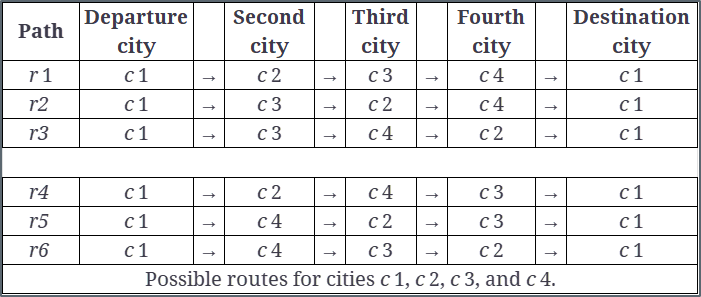
\includegraphics[keepaspectratio]{Pictures/tsp1.png}}
\item
  Different paths for a truck driver in the case of four cities.
\end{itemize}

\begin{Shaded}
\begin{Highlighting}[]
\ImportTok{import}\NormalTok{ numpy }\ImportTok{as}\NormalTok{ np}
\ImportTok{from}\NormalTok{ scipy.special }\ImportTok{import}\NormalTok{ factorial}

\CommentTok{\# TSP paths calculation}
\NormalTok{np.set\_printoptions(suppress}\OperatorTok{=}\VariableTok{True}\NormalTok{)}
\NormalTok{n }\OperatorTok{=}\NormalTok{ np.arange(}\DecValTok{4}\NormalTok{, }\DecValTok{12}\NormalTok{)}
\NormalTok{result }\OperatorTok{=}\NormalTok{ factorial(n }\OperatorTok{{-}} \DecValTok{1}\NormalTok{) }\OperatorTok{/} \DecValTok{2}
\BuiltInTok{print}\NormalTok{(result)  }\CommentTok{\# Expected output: [3, 12, 60, 360, 2520, 20160, 181440, 1814400]}
\end{Highlighting}
\end{Shaded}

\begin{verbatim}
[      3.      12.      60.     360.    2520.   20160.  181440. 1814400.]
\end{verbatim}

\begin{itemize}
\tightlist
\item
  The number of routes are listed below in table form.
\end{itemize}

\begin{figure}[H]

{\centering \pandocbounded{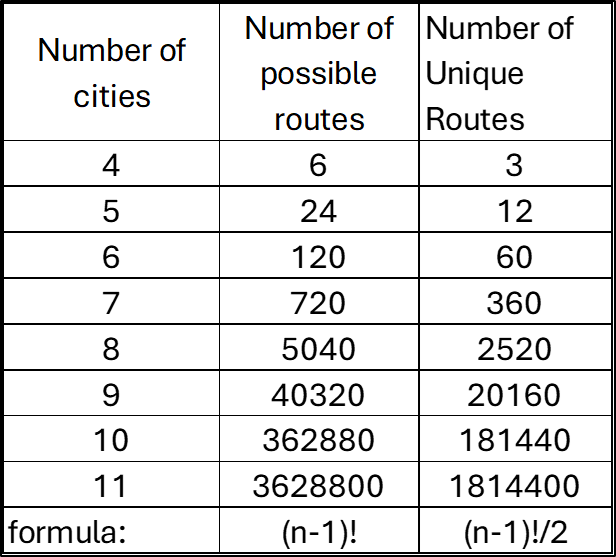
\includegraphics[keepaspectratio]{Pictures/tsp.png}}

}

\caption{tsp routes}

\end{figure}%

\bookmarksetup{startatroot}

\chapter{What are Heuristics?}\label{what-are-heuristics}

\begin{itemize}
\tightlist
\item
  Heuristics are problem-solving methods that use a practical approach
  to reach solutions or decisions more quickly.
\item
  Characteristics: Simplified rules, shortcuts, or educated guesses that
  may not guarantee a perfect solution but are efficient.
\item
  Application: Useful for making quick decisions when data is incomplete
  or when computational resources are limited.
\item
  Speed vs.~Accuracy Trade-off
\item
  Real-world applications where exact solutions are impractical
\end{itemize}

\bookmarksetup{startatroot}

\chapter{Heuristic Algorithms}\label{heuristic-algorithms}

\begin{itemize}
\tightlist
\item
  Algorithms

  \begin{itemize}
  \tightlist
  \item
    A sequence of steps providing a solution
  \end{itemize}
\item
  ``Heuristic''

  \begin{itemize}
  \tightlist
  \item
    Not necessarily optimal, or ``approximate''
  \end{itemize}
\item
  Heuristic Algorithms are used when optimal methods take too long, and
  a timely answer required for effective action.
\end{itemize}

\bookmarksetup{startatroot}

\chapter{Types of Heuristic Methods}\label{types-of-heuristic-methods}

\begin{itemize}
\tightlist
\item
  Constructive Heuristics

  \begin{itemize}
  \tightlist
  \item
    Builds a solution step-by-step.
  \item
    Example: Greedy Algorithms -- making the best choice at each step.
  \end{itemize}
\item
  Improvement Heuristics

  \begin{itemize}
  \tightlist
  \item
    Starts with an initial solution and makes iterative improvements.
  \item
    Example: Local Search -- tweaking solutions to find better ones.
  \end{itemize}
\item
  Metaheuristics

  \begin{itemize}
  \tightlist
  \item
    Higher-level procedures guiding other heuristics.
  \item
    Example: Genetic Algorithms, Simulated Annealing.
  \end{itemize}
\end{itemize}

\bookmarksetup{startatroot}

\chapter{Why Metaheuristics?}\label{why-metaheuristics}

\begin{itemize}
\tightlist
\item
  Unlike generating and checking all the candidate solutions
  systematically, the basic idea of metaheuristics is to find an
  approximate solution out of a very large solution space for a complex
  problem in a ``reasonable time'' via a ``strategic guess.''
\item
  For most complex optimization problems, modern computers are incapable
  of finding the best solution using exhaustive search (ES) because the
  number of possible candidate solutions is simply way too large to be
  checked in a reasonable time.
\item
  As long as it is impossible to check all solutions in the solution
  space of a complex optimization problem in a reasonable time,
  metaheuristic algorithms provide a possible solution to the problem in
  the sense that an approximate, or even optimal, solution can be found
  in a reasonable time.
\item
  Unlike generating and checking all the candidate solutions
  systematically, the basic idea of metaheuristics is to find an
  approximate solution out of a very large solution space for a complex
  problem in a ``reasonable time'' via a ``strategic guess.''
\end{itemize}

\bookmarksetup{startatroot}

\chapter{Organization and Structure of the Metaheuristics
Book}\label{organization-and-structure-of-the-metaheuristics-book}

\begin{figure}[H]

{\centering \pandocbounded{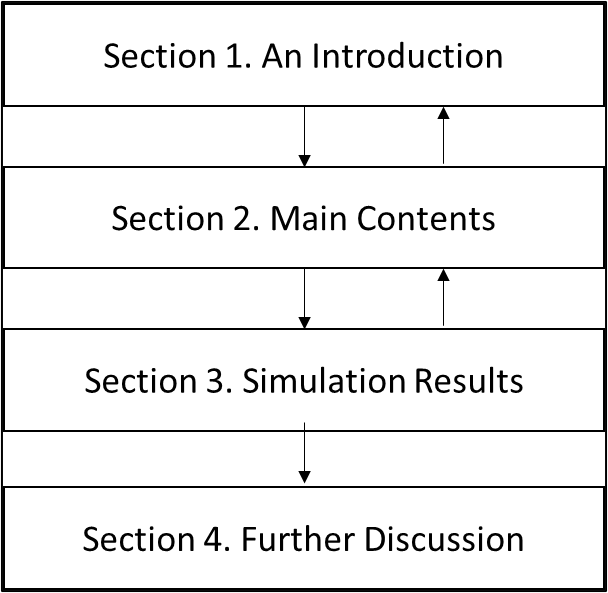
\includegraphics[keepaspectratio]{Pictures/Ch1Book.png}}

}

\caption{Book Overview}

\end{figure}%%
\begin{figure}[H]

{\centering \pandocbounded{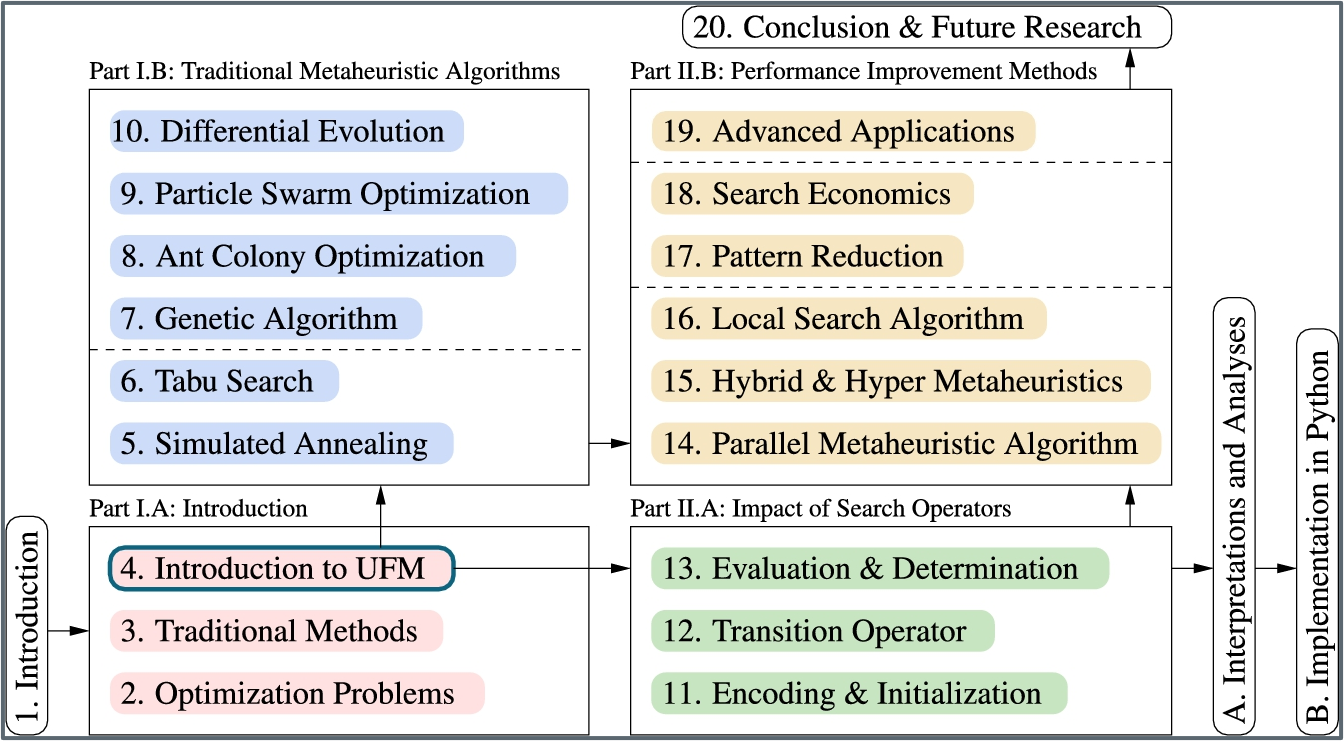
\includegraphics[keepaspectratio]{Pictures/Ch1Book2.png}}

}

\caption{Book Overview}

\end{figure}%

\bookmarksetup{startatroot}

\chapter{What We Cover}\label{what-we-cover}

\begin{itemize}
\item
  How to Write and Read and Algorithm
\item
  Summary of Optimization
\item
  Travelling Salesman
\item
  Greedy Algorithm
\item
  Some Benchmark Problems
\item
  Exhaustive Search
\item
  Hill Climbing
\item
  Metaheuristics

  \begin{itemize}
  \tightlist
  \item
    Simulated Annealing
  \item
    Genetic Algorithm
  \end{itemize}
\item
  Algorithm -\textgreater{} Pseudocode -\textgreater{} Implementation in
  Python
  \pandocbounded{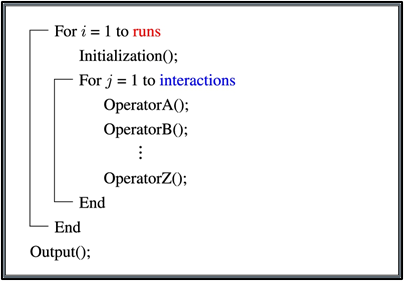
\includegraphics[keepaspectratio]{Pictures/Ch1Pseudo.png}}
\end{itemize}

\bookmarksetup{startatroot}

\chapter{A family tree of metaheuristic
algorithms}\label{a-family-tree-of-metaheuristic-algorithms}

\begin{itemize}
\item
  Besides summarizing Optimization and Heuristic Models, we will cover
  Simulated Annealing and Genetic Algorithms.
\item
  Local Search-Based Metaheuristics

  \begin{itemize}
  \tightlist
  \item
    Aim: Incrementally improve solutions by exploring the neighborhood
    of the current solution.
  \item
    Hill Climbing
  \item
    Simulated Annealing: Inspired by the annealing process in
    metallurgy. Balances exploration (random moves) and exploitation
    (accepting improvements), with a temperature parameter to control
    randomness.
  \item
    Tabu Search: Uses memory structures to avoid revisiting recently
    explored solutions.
  \end{itemize}
\item
  Evolutionary Computation

  \begin{itemize}
  \tightlist
  \item
    Aim: Mimic natural evolutionary processes, working with populations
    of solutions.
  \item
    Genetic Algorithms (GA): Inspired by natural selection, combining
    selection, crossover, and mutation operators to evolve solutions.
  \item
    Differential Evolution: Operates by recombining population members
    based on differences between solution vectors.
  \end{itemize}
\item
  Swarm Intelligence

  \begin{itemize}
  \tightlist
  \item
    Ant Colony Optimization (ACO): Mimics the foraging behavior of ants,
    using pheromone trails to guide the search.
  \item
    Cuckoo Search: Inspired by the brood parasitism of cuckoos.
  \item
    Particle Swarm Optimization (PSO): Inspired by social behaviors of
    animals, where individuals adjust their positions based on personal
    and social information.
  \item
    Artificial Bee Colony Algorithm: Based on foraging behavior of bees,
    balancing local and global search.
  \item
    Firefly Algorithm: Inspired by the attraction behavior of fireflies.
  \item
    Whale Optimization Algorithm: Mimics the bubble-net feeding behavior
    of humpback whales.
  \end{itemize}
\item
  Human Intelligence

  \begin{itemize}
  \tightlist
  \item
    Harmony Search: Mimics the improvisation process of musicians,
    balancing between memory considerations and random adjustments.
  \end{itemize}
\item
  Nature-Inspired Algorithms: Inspired by various natural and biological
  phenomena.

  \begin{itemize}
  \tightlist
  \item
    Artificial Immune System: Models the immune response, maintaining
    diversity and adapting to threats.
  \item
    Flower Pollination Algorithm: The Flower Pollination Algorithm (FPA)
    is a nature-inspired optimization technique based on the pollination
    behavior of flowering plants.
  \end{itemize}
\end{itemize}

\bookmarksetup{startatroot}

\chapter{A Critical Question}\label{a-critical-question}

\begin{itemize}
\tightlist
\item
  How do we choose an applicable metaheuristic algorithm for an
  optimization problem in question?
\end{itemize}

\bookmarksetup{startatroot}

\chapter{Algorithm Design and
Pseudocode}\label{algorithm-design-and-pseudocode}

\bookmarksetup{startatroot}

\chapter{\texorpdfstring{\emph{Automate This} by Christopher
Steiner}{Automate This by Christopher Steiner}}\label{automate-this-by-christopher-steiner}

\begin{itemize}
\tightlist
\item
  An algorithm is a set of operations (mathematical, technical) to be
  conducted in a certain sequence to achieve a certain goal.
\item
  The rise of algorithms and their transformative impact on industries.
\item
  Algorithms have gone from being a tool used by a few specialists to
  becoming a driving force in business, finance, healthcare, and more.
\item
  Automation through algorithms is reshaping the world, with both
  positive and negative implications.
\end{itemize}

\section{Algorithms Key Concepts and
Examples}\label{algorithms-key-concepts-and-examples}

\begin{itemize}
\tightlist
\item
  Algorithms in Finance: High-Frequency Trading (HFT) revolutionized
  Wall Street by executing trades at lightning speeds, leading to both
  massive profits and new risks.
\item
  Algorithms in Healthcare: Algorithms that diagnose diseases faster and
  more accurately than doctors.
\item
  Music: Algorithms used by platforms like Pandora to predict and
  recommend songs.
\item
  Impact on Jobs: Automation's role in replacing jobs traditionally done
  by humans, particularly in industries like finance, journalism, and
  even art.
\end{itemize}

\section{Future Implications and Ethical
Considerations}\label{future-implications-and-ethical-considerations}

\begin{itemize}
\tightlist
\item
  Expansion of Algorithms: The growing reach of algorithms in
  decision-making processes, from hiring practices to legal judgments.
\item
  Ethical Concerns: The potential for bias in algorithms and the
  importance of transparency in their design. The need for regulation
  and oversight as algorithms increasingly influence critical aspects of
  life.
\item
  Looking Ahead: Steiner's call for society to adapt to the new
  algorithm-driven world, balancing innovation with ethical
  responsibility.
\end{itemize}

\section{Bias in Algorithms Explored}\label{bias-in-algorithms-explored}

\begin{itemize}
\tightlist
\item
  Facial Recognition Technology algorithms have shown significant
  biases, particularly in accurately identifying people of different
  races and genders.

  \begin{itemize}
  \tightlist
  \item
    Studies have found that some facial recognition systems have higher
    error rates when identifying individuals with darker skin tones and
    women. This can lead to discriminatory outcomes, such as
    misidentifying people of color at higher rates than white
    individuals.
  \item
    Impact: This bias can result in wrongful accusations or the
    exclusion of certain groups from services that rely on facial
    recognition technology.
  \end{itemize}
\item
  Hiring algorithms are used by companies to screen job applicants, but
  they can unintentionally perpetuate biases present in the training
  data.

  \begin{itemize}
  \tightlist
  \item
    A famous case involved an AI hiring tool developed by Amazon, which
    was found to be biased against female applicants. The algorithm was
    trained on resumes submitted over the previous decade, which were
    predominantly from male applicants, leading the AI to favor male
    candidates.
  \item
    Impact: This bias can reinforce gender inequalities in the workplace
    by systematically disadvantaging qualified female applicants.
  \end{itemize}
\item
  Predictive Policing algorithms analyze historical crime data to
  predict where future crimes are likely to occur, influencing law
  enforcement patrols.

  \begin{itemize}
  \tightlist
  \item
    These algorithms often reflect existing biases in policing
    practices, such as disproportionately targeting minority
    neighborhoods. Because the training data may contain biased policing
    patterns, the algorithm can perpetuate over-policing in certain
    communities.
  \item
    Impact: This can lead to a cycle of increased surveillance and
    criminalization of specific racial or ethnic groups, reinforcing
    systemic biases in the criminal justice system.
  \end{itemize}
\end{itemize}

\bookmarksetup{startatroot}

\chapter{How to Design an Algorithm:}\label{how-to-design-an-algorithm}

\begin{itemize}
\tightlist
\item
  A Routing Problem: Find a good path from Williamsburg to Los Angeles
\end{itemize}

\begin{figure}[H]

{\centering \pandocbounded{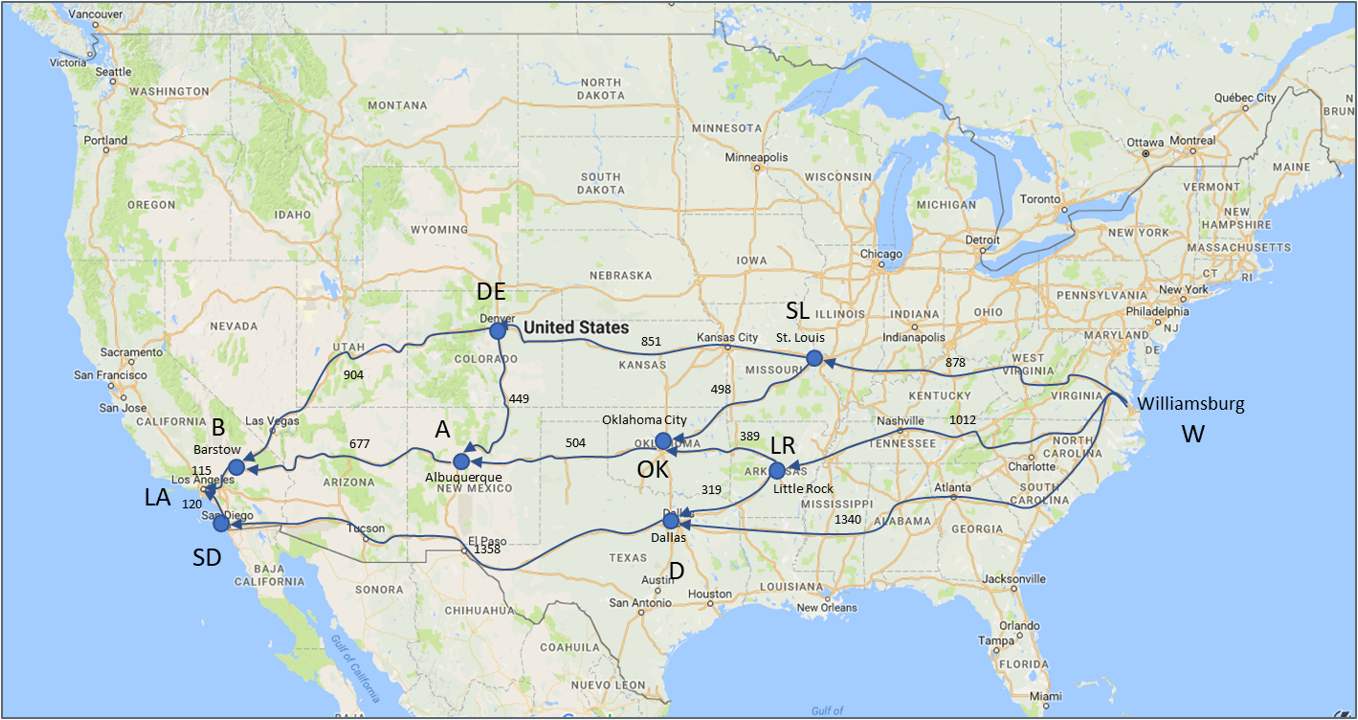
\includegraphics[keepaspectratio]{Pictures/Routing.png}}

}

\caption{Routing Chart}

\end{figure}%

\section{Algorithm Development
Process:}\label{algorithm-development-process}

\begin{itemize}
\item
  What should you do first?
\item
  0: Think of a conceptual approach
\item
  1: Write step-by-step outline

  \begin{itemize}
  \tightlist
  \item
    In words (maybe pseudo code)
  \item
    Focus on sound logic
  \end{itemize}
\item
  2: Plan programming implementation

  \begin{itemize}
  \tightlist
  \item
    Choose appropriate data structures + Speed, memory, convenience
  \item
    Consider functions, which kind of loops
  \end{itemize}
\item
  3: Write the program and debug

  \begin{itemize}
  \tightlist
  \item
    Use the outline as comment statements
  \item
    Write your algorithms in chunks, write a line, then test it
  \end{itemize}
\end{itemize}

\begin{figure}[H]

{\centering \pandocbounded{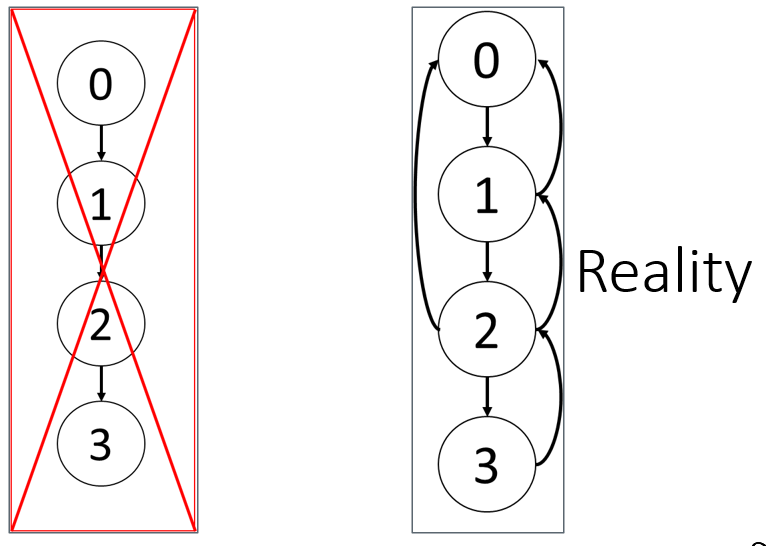
\includegraphics[keepaspectratio]{Pictures/process.png}}

}

\caption{Process}

\end{figure}%

\section{Understanding the Structure of
Algorithms}\label{understanding-the-structure-of-algorithms}

\begin{itemize}
\tightlist
\item
  Identify the Purpose:

  \begin{itemize}
  \tightlist
  \item
    Start by understanding what the algorithm is supposed to achieve.
  \item
    Look for a brief description or goal at the beginning.
  \end{itemize}
\item
  Break Down the Steps:

  \begin{itemize}
  \tightlist
  \item
    Algorithms are typically presented as a sequence of steps.
  \item
    Each step corresponds to a specific action or decision.
  \item
    in words. Focus on sound logic.
  \end{itemize}
\item
  Recognize Input and Output:

  \begin{itemize}
  \tightlist
  \item
    Determine what inputs the algorithm requires.
  \item
    Identify the expected output(s) after the algorithm is executed.
  \end{itemize}
\end{itemize}

\section{Understanding the Structure of Algorithms: Flow
Control}\label{understanding-the-structure-of-algorithms-flow-control}

\begin{itemize}
\tightlist
\item
  Determine how the algorithm progresses through its steps and notice
  the flow control structures like loops (for, while) and conditionals
  (if, else).

  \begin{itemize}
  \tightlist
  \item
    Which data types?

    \begin{itemize}
    \tightlist
    \item
      Begin to consider speed, memory usage, convenience tradeoffs
    \end{itemize}
  \item
    Finer details of data organization

    \begin{itemize}
    \tightlist
    \item
      What fields for dictionary labels?
    \item
      How should lists be sorted, if at all?
    \end{itemize}
  \item
    Loop types

    \begin{itemize}
    \tightlist
    \item
      for or while?
    \item
      Ease of coding and development
    \end{itemize}
  \item
    Use functions?
  \end{itemize}
\end{itemize}

\bookmarksetup{startatroot}

\chapter{Deciphering Algorithmic
Notation}\label{deciphering-algorithmic-notation}

\begin{itemize}
\tightlist
\item
  Variables and Data Types:

  \begin{itemize}
  \tightlist
  \item
    Identify variables and understand their roles (e.g., counters,
    accumulators).
  \item
    Pay attention to the data types being used (e.g., integers, lists).
  \end{itemize}
\item
  Lists

  \begin{itemize}
  \tightlist
  \item
    Good if you are going to iterate through the entire list
  \item
    Methods: sort, iterable, reverse, append
  \end{itemize}
\item
  Tuples

  \begin{itemize}
  \tightlist
  \item
    Similar to lists, but when the data shouldn't change
  \item
    Immutable
  \item
    Not many built-in methods
  \end{itemize}
\item
  Dictionaries

  \begin{itemize}
  \tightlist
  \item
    Fast random access: lookup by key
  \item
    Takes a little more memory than lists
  \end{itemize}
\end{itemize}

\section{Deciphering Algorithmic Notation: Pseudocode
vs.~Code}\label{deciphering-algorithmic-notation-pseudocode-vs.-code}

\begin{itemize}
\tightlist
\item
  Recognize that many algorithms are written in pseudocode, a high-level
  description that isn't tied to any specific programming language.
\item
  Some feel that with Python, the pseudo-code step would not be
  necessary anymore
\item
  Translate pseudocode into actual code if needed.

  \begin{itemize}
  \tightlist
  \item
    Program in chunks
  \item
    Test each chunk before moving on
  \item
    Use functions where reasonable

    \begin{itemize}
    \tightlist
    \item
      Easier to test
    \end{itemize}
  \end{itemize}
\item
  Check code where solutions are known

  \begin{itemize}
  \tightlist
  \item
    Small problems
  \item
    Obvious solutions
  \end{itemize}
\item
  Check code as you write it
\item
  Debug Often

  \begin{itemize}
  \tightlist
  \item
    Breakpoints
  \item
    Check variables in console
  \item
    Variable explorer
  \item
    Print statements
  \end{itemize}
\end{itemize}

\section{Deciphering Algorithmic Notation: Mathematical
Symbols}\label{deciphering-algorithmic-notation-mathematical-symbols}

\begin{itemize}
\tightlist
\item
  Mathematical Symbols:

  \begin{itemize}
  \tightlist
  \item
    Algorithms often include mathematical notation, such as sums
    (\(\sum\)) or products (\(\prod\)).
  \item
    Understand these as they relate to the algorithm's operations.
  \end{itemize}
\item
  Big-O Notation:

  \begin{itemize}
  \tightlist
  \item
    Look for references to Big-O notation, which indicates the
    algorithm's efficiency in terms of time or space.
  \item
    Understand the implications for performance, especially with large
    inputs.
  \end{itemize}
\item
  Commenting

  \begin{itemize}
  \tightlist
  \item
    Commenting improves code readability, reuse, and maintainability.
  \item
    Can transfer algorithm outline to a program as comments.
  \item
    Then, you have comments that provide an outline for coding.
  \end{itemize}
\end{itemize}

\section{Design Paradigms}\label{design-paradigms}

\begin{itemize}
\tightlist
\item
  Algorithms can be based on:

  \begin{itemize}
  \tightlist
  \item
    Intuitive ideas
  \item
    Math
  \end{itemize}
\item
  Optimization

  \begin{itemize}
  \tightlist
  \item
    Possibly with calculus analysis (e.g., gradients)
  \item
    Heuristic model analysis
  \item
    Dynamic programming
  \end{itemize}
\end{itemize}

\bookmarksetup{startatroot}

\chapter{Introduction to Algorithm
Symbols}\label{introduction-to-algorithm-symbols}

\begin{itemize}
\tightlist
\item
  \textbf{Variables}: Represent inputs, outputs, or intermediate values.

  \begin{itemize}
  \tightlist
  \item
    (\(x\)): A common symbol for an input variable.
  \item
    (\(y\)): Often represents an output variable.
  \item
    (\(i\), \(j\), \(k\)): Typically used as indices in loops.
  \end{itemize}
\item
  \textbf{Sets}: Collections of elements.

  \begin{itemize}
  \tightlist
  \item
    (\(S\)): A set, e.g., ( S = \{1, 2, 3\} ).
  \item
    (\(\mathbb{N}\)): The set of natural numbers.
  \item
    (\(\in\)): ``An element of'', used to denote membership in a set.
  \end{itemize}
\item
  \textbf{Operators}: Perform operations on variables or sets.

  \begin{itemize}
  \tightlist
  \item
    (\(+, -, \times, /\) ): Basic arithmetic operators.
  \item
    (\(\cup\)): Union of two sets.
  \item
    (\(\cap\)): Intersection of two sets.
  \item
    (\(\subseteq\)): Subset relation.
  \end{itemize}
\end{itemize}

\begin{center}\rule{0.5\linewidth}{0.5pt}\end{center}

\section{Common Symbols in
Algorithms}\label{common-symbols-in-algorithms}

\begin{itemize}
\tightlist
\item
  \textbf{Mathematical Symbols}:

  \begin{itemize}
  \tightlist
  \item
    \(\forall\): ``For all'', used in universal quantification.
  \item
    \(\exists\): ``There exists'', used in existential quantification.
  \item
    \(\sum_{i=1}^n x_i\): Summation from \(i = 1\) to \(n\).
  \item
    \(\prod_{i=1}^n x_i\): Product from \(i = 1\) to \(n\).
  \end{itemize}
\item
  \textbf{Logical Symbols}:

  \begin{itemize}
  \tightlist
  \item
    \(\land\): Logical AND.
  \item
    \(\lor\): Logical OR.
  \item
    \(\neg\): Logical NOT.
  \item
    \(\implies\): Logical implication.
  \end{itemize}
\item
  \textbf{Algorithm-Specific Notation}:

  \begin{itemize}
  \tightlist
  \item
    \(O(n)\): Big-O notation, representing algorithm complexity.
  \item
    \(P \leftarrow Q\): Assign the value of \(Q\) to \(P\).
  \item
    \textbf{for} \(i = 1\) \textbf{to} \(n\): A loop from \(i = 1\) to
    \(n\).
  \item
    \textbf{if} \((condition)\): A conditional statement.
  \end{itemize}
\end{itemize}

\section{Summation and Loop Example}\label{summation-and-loop-example}

\begin{itemize}
\item
  \textbf{Summation Formula}:
  \(S = \sum_{i=1}^{n} i = 1 + 2 + 3 + \dots + n\)

  \begin{itemize}
  \tightlist
  \item
    \textbf{Explanation}: This formula calculates the sum of the first
    \(n\) natural numbers. The symbol \(\sum\) represents the summation,
    and \(i\) is the index that runs from 1 to \(n\).
  \end{itemize}
\item
  \textbf{Nested Loop Calculation}:
  \(T = \sum_{i=1}^{n} \sum_{j=1}^{m} (i \times j)\)

  \begin{itemize}
  \tightlist
  \item
    \textbf{Explanation}: This formula represents a nested summation
    where \(i\) runs from 1 to \(n\) and \(j\) runs from 1 to \(m\). It
    calculates the sum of the product of \(i\) and \(j\) over these
    ranges.
  \end{itemize}
\end{itemize}

\begin{center}\rule{0.5\linewidth}{0.5pt}\end{center}

\section{Conditional Statements and
Recursion}\label{conditional-statements-and-recursion}

\begin{itemize}
\item
  \textbf{Conditional Formula}: \[
  f(x) = 
  \begin{cases} 
  0 & \text{if } x < 0 \\
  1 & \text{if } x \geq 0
  \end{cases}
  \]

  \begin{itemize}
  \tightlist
  \item
    \textbf{Explanation}: This piecewise function returns 0 if ( x ) is
    less than 0, and 1 if ( x ) is greater than or equal to 0. It's an
    example of a conditional statement in algorithmic form.
  \end{itemize}
\item
  \textbf{Recursive Formula}: \[
  F(n) = 
  \begin{cases}
  1 & \text{if } n = 1 \\
  n \times F(n-1) & \text{if } n > 1
  \end{cases}
  \]

  \begin{itemize}
  \tightlist
  \item
    \textbf{Explanation}: This is a recursive definition of the
    factorial function. For ( n = 1 ), ( F(n) = 1 ). For ( n
    \textgreater{} 1 ), ( F(n) ) is defined as ( n ) times the factorial
    of ( n-1 ).
  \end{itemize}
\end{itemize}

\begin{center}\rule{0.5\linewidth}{0.5pt}\end{center}

\section{Big-O Notation and Algorithm
Complexity}\label{big-o-notation-and-algorithm-complexity}

\begin{itemize}
\item
  \textbf{Big-O Notation Example}: \(T(n) = O(n^2)\)

  \begin{itemize}
  \tightlist
  \item
    \textbf{Explanation}: This formula describes the time complexity of
    an algorithm, where\(T(n)\) represents the runtime as a function of
    input size \(n\). The notation \(O(n^2)\) indicates that the
    algorithm's runtime grows quadratically with the size of the input.
  \end{itemize}
\item
  \textbf{Logarithmic Complexity}: \(T(n) = O(\log n)\)

  \begin{itemize}
  \tightlist
  \item
    \textbf{Explanation}: This formula represents an algorithm with
    logarithmic time complexity. The runtime increases logarithmically
    as the input size \(n\) increases, which is common in algorithms
    like binary search.
  \end{itemize}
\end{itemize}

\section{Basic TSP Formulation}\label{basic-tsp-formulation}

\begin{itemize}
\item
  \textbf{Objective Function}: \[
  \text{Minimize} \quad Z = \sum_{i=1}^{n} \sum_{j=1, j \neq i}^{n} c_{ij} x_{ij}
   \]

  \begin{itemize}
  \tightlist
  \item
    \textbf{Explanation}: This formula represents the objective function
    of the TSP, where \(c_{ij}\) is the cost (or distance) of traveling
    from city \(i\) to city \(j\), and \(x_{ij}\) is a binary variable
    that equals 1 if the path from \(i\) to \(j\) is included in the
    solution and 0 otherwise. The goal is to minimize the total travel
    cost.
  \end{itemize}
\item
  \textbf{Constraints}:
\item
  \(\sum_{j=1, j \neq i}^{n} x_{ij} = 1 \quad \forall i\)
\item
  \(\sum_{i=1, i \neq j}^{n} x_{ij} = 1 \quad \forall j\)
\item
  \(x_{ij} \in \{0, 1\}\)

  \begin{itemize}
  \tightlist
  \item
    \textbf{Explanation}: The first constraint ensures that each city
    \(i\) is exited exactly once, and the second constraint ensures that
    each city \(j\) is entered exactly once. The binary constraint on
    \(x_{ij}\) ensures that the solution only includes valid paths.
  \end{itemize}
\end{itemize}

\begin{center}\rule{0.5\linewidth}{0.5pt}\end{center}

\section{TSP Approximation Algorithm}\label{tsp-approximation-algorithm}

\begin{itemize}
\item
  \textbf{Approximation Algorithm Cost}: \(Z \leq 2 \times \text{OPT}\)

  \begin{itemize}
  \tightlist
  \item
    \textbf{Explanation}: This formula represents the performance
    guarantee of a 2-approximation algorithm for the TSP, where \(Z\) is
    the cost of the approximate solution and \(\text{OPT}\) is the cost
    of the optimal solution. It guarantees that the approximate solution
    will be at most twice as costly as the optimal solution.
  \end{itemize}
\end{itemize}

\section{Heuristic Nearest Neighbor
Example:}\label{heuristic-nearest-neighbor-example}

\(Z = \sum_{i=1}^{n-1} c_{i, \text{NN}(i)} + c_{n, \text{NN}(1)}\)

\begin{itemize}
\tightlist
\item
  \textbf{Explanation}: This is the cost calculation for the nearest
  neighbor heuristic, where \(\text{NN}(i)\) denotes the nearest
  neighbor of city \(i\). The tour starts at a city, repeatedly visits
  the nearest unvisited city, and returns to the starting city.
\end{itemize}

\section{Activity:}\label{activity}

\begin{itemize}
\tightlist
\item
  State what the following algorithms do:
\end{itemize}

\[Z = \sum_{i=1}^n \left( x_i \times y_i \right)\]
\[ \bar{X} = \frac{\sum_{i=1}^{n} w_i x_i}{\sum_{i=1}^{n} w_i}\]

\bookmarksetup{startatroot}

\chapter{Pseudocode Know-how}\label{pseudocode-know-how}

\begin{itemize}
\item
  Don't include code-specific features such as variable declarations,
  data types, or specific keywords.
\item
  Focus on what the algorithm should do, not how to implement it.
\item
  Use pseudocode to outline the flow and logic of the solution.
\item
  Think of pseudocode as a blueprint that can be implemented in any
  programming language
\item
  Bad: int sum = 0; for (i=0; i \textless{} n; i++) sum += arr{[}i{]};
\item
  Good: SET sum = 0, FOR each element in the list, ADD element to sum
\end{itemize}

\section{Tips for Writing Good
Pseudocode}\label{tips-for-writing-good-pseudocode}

\begin{itemize}
\tightlist
\item
  Maintain consistent terms throughout: Use the same terminology for
  variables, functions, and processes. If you define a variable as
  total, always refer to it as total, not sum later on.
\item
  Be clear on naming: Use descriptive names for variables, functions,
  and operations to make your pseudocode intuitive.
\item
  Pseudocode should be easy to understand after a single read-through.
  If it feels too complex, break it down further.
\end{itemize}

\section{Examples}\label{examples}

\begin{itemize}
\tightlist
\item
  This pseudocode finds the smallest number in a given list by iterating
  through all elements and updating the min\_number whenever a smaller
  number is found.
\end{itemize}

\begin{Shaded}
\begin{Highlighting}[]
\NormalTok{\# Pseudocode for finding the minimum number in a list}
\NormalTok{SET min\_number = Infinity}
\NormalTok{FOR each number IN list:}
\NormalTok{    IF number \textless{} min\_number:}
\NormalTok{        SET min\_number = number}
\NormalTok{RETURN min\_number}
\end{Highlighting}
\end{Shaded}

\begin{itemize}
\tightlist
\item
  This pseudocode below calculates the sum of all numbers in the list
  that are greater than a specified threshold by iterating through the
  list and adding qualifying numbers to the sum.
\item
  edge cases: an empty list, all even numbers, or no numbers greater
  than the threshold.
\end{itemize}

\begin{Shaded}
\begin{Highlighting}[]
\NormalTok{\# Pseudocode for summing numbers greater than a given threshold}
\NormalTok{SET sum = 0}
\NormalTok{FOR each number IN list:}
\NormalTok{    IF number \textgreater{} threshold:}
\NormalTok{        ADD number TO sum}
\NormalTok{RETURN sum}
\end{Highlighting}
\end{Shaded}

\section{Activity: Read this
Pseudocode}\label{activity-read-this-pseudocode}

\begin{Shaded}
\begin{Highlighting}[]
\NormalTok{SET min\_even = Infinity }
\NormalTok{FOR each number IN list: }
\NormalTok{    IF number is even AND number \textless{} min\_even: }
\NormalTok{        SET min\_even = number }
\NormalTok{RETURN min\_even}
\end{Highlighting}
\end{Shaded}

\section{Pseudocode for Basic TSP
Formation}\label{pseudocode-for-basic-tsp-formation}

\begin{itemize}
\tightlist
\item
  Generic Inputs: The pseudocode is now generic and works for any TSP
  model where you have a set of cities and their corresponding
  distances.
\item
  Nearest Neighbor Heuristic: The algorithm works by greedily choosing
  the nearest unvisited city until all cities are visited, then
  returning to the start city.
\item
  Output: It outputs the route and the total distance traveled.
\end{itemize}

\begin{Shaded}
\begin{Highlighting}[]
\NormalTok{\#inputs}
\NormalTok{SET cities = \textless{}list of cities\textgreater{}}
\NormalTok{SET distances = \textless{}distance matrix or dictionary\textgreater{}}
\NormalTok{SET start\_city = \textless{}initial city\textgreater{}}


\NormalTok{\# FUNCTION to find the nearest unvisited city}
\NormalTok{FUNCTION find\_nearest\_neighbor(current\_city, unvisited, distances):}
\NormalTok{    SET nearest\_city = None}
\NormalTok{    SET min\_distance = infinity}
    
\NormalTok{    FOR each city IN unvisited:}
\NormalTok{        IF distances[current\_city][city] \textless{} min\_distance:}
\NormalTok{            SET min\_distance = distances[current\_city][city]}
\NormalTok{            SET nearest\_city = city}
    
\NormalTok{    RETURN nearest\_city, min\_distance}

\NormalTok{\# FUNCTION to solve TSP using Nearest Neighbor algorithm}
\NormalTok{FUNCTION nearest\_neighbor\_tsp(start\_city, cities, distances):}
\NormalTok{\# Initialize list of unvisited cities}
\NormalTok{    SET unvisited = list of all cities EXCEPT start\_city}
\end{Highlighting}
\end{Shaded}

\bookmarksetup{startatroot}

\chapter{Using AI}\label{using-ai}

\begin{itemize}
\item
  Use the following prompt on a generative AI, like chatGPT, to learn
  more about the topics covered.
\item
  Defining Algorithms: Explain, in your own words, what an algorithm is
  and provide an example from everyday life (e.g., a recipe or a set of
  instructions).
\item
  Ethics and Bias: Discuss one example of algorithmic bias, such as
  facial recognition or hiring algorithms. What could be done to address
  these biases?
\item
  Routing Problem: Given a problem like finding the shortest path from
  point A to point B, outline a step-by-step algorithm using pseudocode.
\item
  Flow Control: Illustrate how flow control structures (e.g., loops and
  conditionals) help manage decision-making in algorithms. Provide a
  simple example in pseudocode.
\item
  Optimization Considerations: Discuss how tradeoffs between speed,
  memory usage, and convenience influence algorithm design. Can you
  think of a scenario where one must be prioritized over others?
\item
  Pseudocode to Code: Write a pseudocode for a basic task (e.g.,
  calculating the average of a list of numbers) and then translate it
  into Python code.
\item
  Interpreting Pseudocode: Given a pseudocode example from the slides
  (e.g., the TSP example), explain the purpose and main steps of the
  algorithm.
\item
  Choosing Data Structures: Compare lists, tuples, and dictionaries in
  Python. Provide examples of when each would be the most appropriate
  choice in an algorithm.
\item
  Sorting and Searching: Write pseudocode for a simple sorting algorithm
  (e.g., bubble sort) and explain its time complexity in terms of Big-O
  notation.
\item
  TSP Complexity: Explain why the Traveling Salesman Problem (TSP) is
  computationally challenging. How does the Nearest Neighbor approach
  simplify the problem?
\item
  Algorithm Design Paradigms: Compare heuristic-based algorithms to
  optimization-based approaches. When might a heuristic be preferred
  over an exact method?
\item
  Debugging Steps: What are some strategies to debug algorithms
  effectively during implementation? Share an experience or hypothetical
  scenario where one of these strategies was crucial.
\item
  Ethical Considerations in Practice: Imagine you are tasked with
  designing a hiring algorithm. How would you ensure it is free from
  bias and promotes equity?
\end{itemize}

\bookmarksetup{startatroot}

\chapter{Conclusions}\label{conclusions}

\begin{itemize}
\tightlist
\item
  Resist the urge to start by writing code!!!

  \begin{itemize}
  \tightlist
  \item
    Invest time upfront developing your approach.

    \begin{itemize}
    \tightlist
    \item
      Conceptual and implementation plan.
    \end{itemize}
  \end{itemize}
\item
  The code writes itself if you have a good understanding of the formula
  and good pseudocode.
\item
  More time now planning\ldots{} a lot less time later coding.
\end{itemize}

\bookmarksetup{startatroot}

\chapter{Python for Heuristics \&
NumPy}\label{python-for-heuristics-numpy}

\bookmarksetup{startatroot}

\chapter{Coding Know-How}\label{coding-know-how}

\begin{itemize}
\tightlist
\item
  In the field of heuristic modeling, coding know-how is not just a
  tool---it's an essential skill that enables you to experiment, adapt,
  and optimize solutions for complex, real-world problems. As we explore
  heuristic methods in this MSBA course, having a strong foundation in
  coding, especially in Python, will allow you to implement and test
  algorithms efficiently.
\item
  Good coding practices, such as writing clear, modular code and
  incorporating meaningful comments, are critical for both readability
  and collaboration. By starting with simple Python examples that
  highlight these principles, we'll build the groundwork for more
  sophisticated modeling tasks, from randomization techniques to
  optimization algorithms, equipping you with both technical skills and
  best practices for professional code development.
\end{itemize}

What problems does this code have?
\pandocbounded{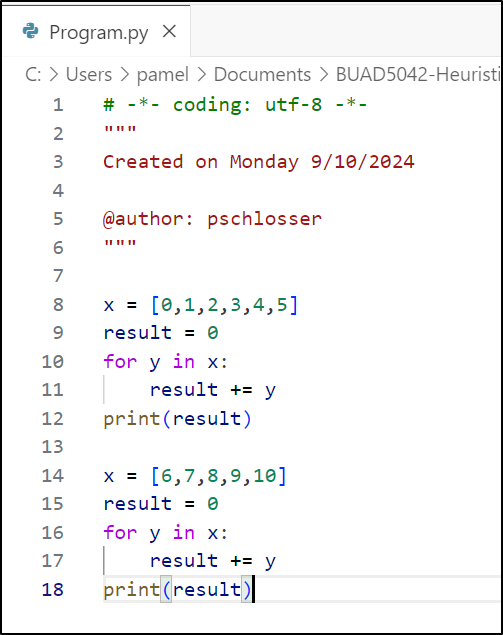
\includegraphics[keepaspectratio]{Pictures/programPY.png}}

\begin{itemize}
\tightlist
\item
  Multiple instantiations of the same code within a program cause
  problems + More opportunities for errors

  \begin{itemize}
  \tightlist
  \item
    More maintenance
  \end{itemize}
\item
  Blocks of reusable code solve this problem

  \begin{itemize}
  \tightlist
  \item
    These are called functions
  \end{itemize}
\item
  To avoid resetting the value of result and preserve the sum of both
  lists, you can accumulate the sums in a single loop or retain the
  value of result between the loops.
\item
  Alternatively, you can use Python's built-in sum() function to
  simplify the code like below.
\end{itemize}

\begin{Shaded}
\begin{Highlighting}[]
\NormalTok{x1 }\OperatorTok{=}\NormalTok{ [}\DecValTok{0}\NormalTok{, }\DecValTok{1}\NormalTok{, }\DecValTok{2}\NormalTok{, }\DecValTok{3}\NormalTok{, }\DecValTok{4}\NormalTok{, }\DecValTok{5}\NormalTok{]}
\NormalTok{x2 }\OperatorTok{=}\NormalTok{ [}\DecValTok{6}\NormalTok{, }\DecValTok{7}\NormalTok{, }\DecValTok{8}\NormalTok{, }\DecValTok{9}\NormalTok{, }\DecValTok{10}\NormalTok{]}

\BuiltInTok{print}\NormalTok{(}\BuiltInTok{sum}\NormalTok{(x1))}
\BuiltInTok{print}\NormalTok{(}\BuiltInTok{sum}\NormalTok{(x2))}
\end{Highlighting}
\end{Shaded}

\begin{verbatim}
15
40
\end{verbatim}

\bookmarksetup{startatroot}

\chapter{Writing Programs with Internal
Functions}\label{writing-programs-with-internal-functions}

\begin{itemize}
\tightlist
\item
  Indentation: Function statements must be indented.
\item
  Arguments: Variables passed from calling program to the function

  \begin{itemize}
  \tightlist
  \item
    a\_list is an argument required by my\_sum\\
  \item
    a\_list assumes value of x passed from main
  \end{itemize}
\item
  Return: a return statement sends variables back to main program\\
\item
  Variable scope: where execution begins

  \begin{itemize}
  \tightlist
  \item
    The first un-indented line that is not a function definition or a
    global variable
  \item
    a\_list is defined only in the function when it runs
  \end{itemize}
\item
  Place all functions above the ``main'' program

  \begin{itemize}
  \tightlist
  \item
    Must be defined before they are used
  \end{itemize}
\end{itemize}

\begin{Shaded}
\begin{Highlighting}[]
\KeywordTok{def}\NormalTok{ my\_sum(a\_list):}
\NormalTok{    result }\OperatorTok{=} \DecValTok{0}
    \ControlFlowTok{for}\NormalTok{ y }\KeywordTok{in}\NormalTok{ a\_list:}
\NormalTok{        result }\OperatorTok{+=}\NormalTok{ y}
    \ControlFlowTok{return}\NormalTok{ result}
    
\NormalTok{x }\OperatorTok{=}\NormalTok{ [}\DecValTok{0}\NormalTok{,}\DecValTok{1}\NormalTok{,}\DecValTok{2}\NormalTok{,}\DecValTok{3}\NormalTok{,}\DecValTok{4}\NormalTok{,}\DecValTok{5}\NormalTok{]}
\BuiltInTok{print}\NormalTok{(my\_sum(x))}
\end{Highlighting}
\end{Shaded}

\begin{verbatim}
15
\end{verbatim}

\bookmarksetup{startatroot}

\chapter{Understanding The Loop}\label{understanding-the-loop}

\begin{Shaded}
\begin{Highlighting}[]
\NormalTok{for y in a\_list:}
\NormalTok{   result += y}
\NormalTok{return result}
\end{Highlighting}
\end{Shaded}

\begin{itemize}
\tightlist
\item
  A loop is a way to repeat the same action for every item in a
  collection (like a list).
\item
  For y in a\_list means, take each item in a\_list one at a time, and
  call it y.

  \begin{itemize}
  \tightlist
  \item
    For example, if a\_list is {[}0, 1, 2, 3, 4, 5{]}, the loop will do
    the following:
  \item
    First loop: set y = 0, result = 0 + 0 (result is now 0).
  \item
    Second loop: Then, set y = 1, result = 0 + 1 (result is now 1).
  \item
    Third loop: then y = 2, result = 1 + 2 (result is now 3). and so on,
    until all the numbers in the list have been used.
  \end{itemize}
\end{itemize}

\begin{figure}[H]

{\centering \pandocbounded{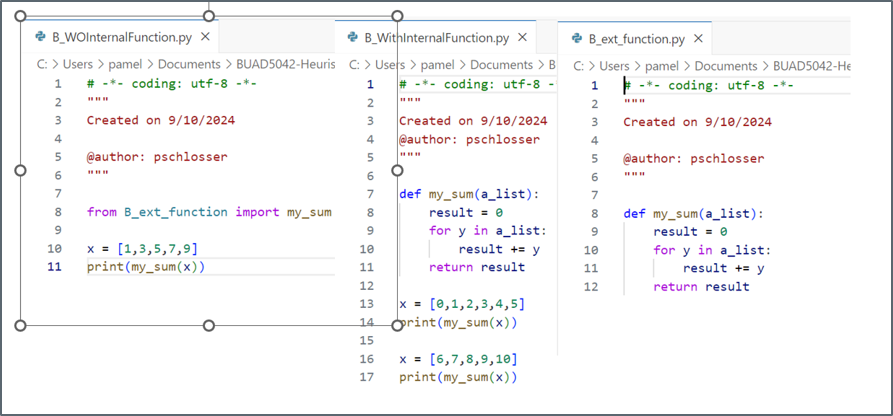
\includegraphics[keepaspectratio]{Pictures/programs.png}}

}

\caption{program.py}

\end{figure}%

\bookmarksetup{startatroot}

\chapter{Object Oriented Programming (OOP) vs Procedural
Programming}\label{object-oriented-programming-oop-vs-procedural-programming}

\begin{itemize}
\tightlist
\item
  Procedural Programming:

  \begin{itemize}
  \tightlist
  \item
    In Python, you can program .py files where the code is organized
    into functions, with data often being passed around between them.
  \item
    Functions perform specific tasks but do not group behavior and state
    (data) together.
  \item
    All the code tends to be written in one or a few large files,
    without much encapsulation or separation of concerns.
  \item
    The textbook uses OOP, I will supplement with procedural models.
  \end{itemize}
\item
  Object Oriented Programming (OOP):

  \begin{itemize}
  \tightlist
  \item
    In Python, you can also use OOP to separate different parts of your
    code, such as algorithms, test cases, and libraries, by
    encapsulating them in different classes or modules. This leads to a
    more organized and maintainable codebase.
  \item
    What can you separate:

    \begin{itemize}
    \tightlist
    \item
      Algorithm (Core Logic): You encapsulate the algorithm or formula
      into a class or function within a class.
    \item
      Library (Utility Functions):Any utility functions or reusable
      logic can be put into a separate class (or module) that handles
      common operations.
    \item
      Test Cases (Validation):Testing is often done through separate
      classes or functions, typically in a separate module.
    \end{itemize}
  \end{itemize}
\end{itemize}

\bookmarksetup{startatroot}

\chapter{Libraries to Note}\label{libraries-to-note}

\begin{figure}[H]

{\centering \pandocbounded{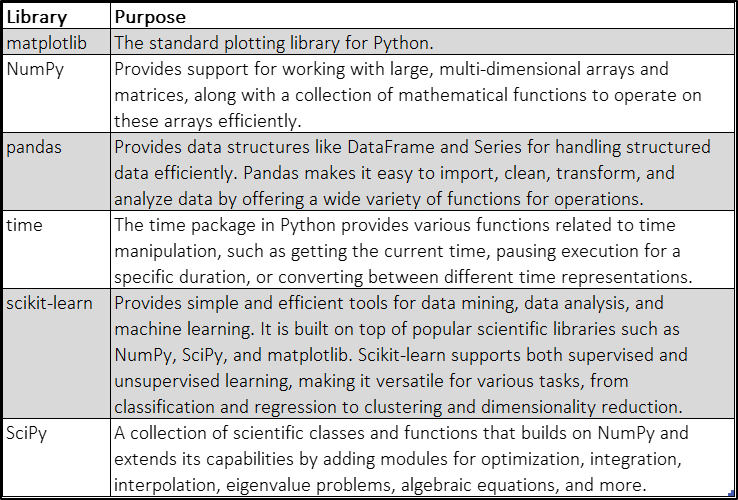
\includegraphics[keepaspectratio]{Pictures/library.png}}

}

\caption{libraries.py}

\end{figure}%

\bookmarksetup{startatroot}

\chapter{Numpy Basics}\label{numpy-basics}

\begin{itemize}
\tightlist
\item
  NumPy stands for numerical Python, suggesting that it targets
  scenarios that are numerically demanding. The base Python interpreter
  tries to be as general as possible in many areas, which often leads to
  quite a bit of overhead at run-time.
\item
  NumPy uses specialization for numerical components as its major
  approach to avoid overhead and to be as good and as fast as possible
  in certain application scenarios.
\item
  Vectorization is a powerful concept for writing concise, easy-to-read,
  and easy-to-maintain code in fields such as finance and algorithmic
  trading. With NumPy, vectorized code does not only make code more
  concise, but it also can speed up code execution considerably (by a
  factor of about eight in the Monte Carlo simulation, for example).
\end{itemize}

\begin{Shaded}
\begin{Highlighting}[]
\ImportTok{import}\NormalTok{ numpy }\ImportTok{as}\NormalTok{ np}
\end{Highlighting}
\end{Shaded}

\section{Basic Array Creation}\label{basic-array-creation}

\begin{itemize}
\tightlist
\item
  The np.array function in NumPy is used to create an array (a grid of
  values) from data provided as lists, tuples, or other array-like
  structures. The resulting NumPy array is a powerful and flexible
  structure for mathematical operations, as it supports multiple
  dimensions, broadcasting, and various data types.
\end{itemize}

\begin{Shaded}
\begin{Highlighting}[]
\CommentTok{\# Creating a simple numpy array from a Python list}
\NormalTok{array }\OperatorTok{=}\NormalTok{ np.array([}\DecValTok{1}\NormalTok{, }\DecValTok{2}\NormalTok{, }\DecValTok{3}\NormalTok{, }\DecValTok{4}\NormalTok{])}
\BuiltInTok{print}\NormalTok{(}\StringTok{"Array:"}\NormalTok{, array)}
\end{Highlighting}
\end{Shaded}

\begin{verbatim}
Array: [1 2 3 4]
\end{verbatim}

\section{Element-Wise Operations}\label{element-wise-operations}

\begin{itemize}
\tightlist
\item
  Element-wise operators are mathematical or logical operations applied
  independently to corresponding elements in arrays or matrices of the
  same shape.
\item
  Each element in one array is combined with the corresponding element
  in the other array using the operator.
\item
  In the context of arrays (such as in NumPy), common element-wise
  operators include basic arithmetic operators:

  \begin{itemize}
  \tightlist
  \item
    Element-wise addition +
  \item
    Element-wise subtraction -
  \item
    Element-wise multiplication *
  \item
    Element-wise division /
  \item
    Element-wise exponentiation **
  \end{itemize}
\end{itemize}

\begin{Shaded}
\begin{Highlighting}[]
\CommentTok{\# Performing element{-}wise addition}
\NormalTok{array }\OperatorTok{=}\NormalTok{ np.array([}\DecValTok{1}\NormalTok{, }\DecValTok{2}\NormalTok{, }\DecValTok{3}\NormalTok{, }\DecValTok{4}\NormalTok{])}
\NormalTok{added\_array }\OperatorTok{=}\NormalTok{ array }\OperatorTok{+} \DecValTok{5}
\BuiltInTok{print}\NormalTok{(}\StringTok{"Added Array:"}\NormalTok{, added\_array)}
\end{Highlighting}
\end{Shaded}

\begin{verbatim}
Added Array: [6 7 8 9]
\end{verbatim}

\begin{Shaded}
\begin{Highlighting}[]
\NormalTok{a }\OperatorTok{=}\NormalTok{ np.array([}\DecValTok{1}\NormalTok{, }\DecValTok{2}\NormalTok{, }\DecValTok{3}\NormalTok{])}
\NormalTok{b }\OperatorTok{=}\NormalTok{ np.array([}\DecValTok{4}\NormalTok{, }\DecValTok{5}\NormalTok{, }\DecValTok{6}\NormalTok{])}
\NormalTok{c }\OperatorTok{=}\NormalTok{ a }\OperatorTok{+}\NormalTok{ b}
\BuiltInTok{print}\NormalTok{(c)}
\end{Highlighting}
\end{Shaded}

\begin{verbatim}
[5 7 9]
\end{verbatim}

\section{Taking an Exponent: np.exp}\label{taking-an-exponent-np.exp}

\begin{itemize}
\tightlist
\item
  np.exp is a function in the NumPy library that calculates the
  exponential of all elements in an input array. Specifically, it
  computes the base-e exponential function, which is 𝑒\^{}𝑥, where 𝑒 is
  Euler's number (approximately 2.71828), and 𝑥 is the input array or
  scalar.
\end{itemize}

\begin{Shaded}
\begin{Highlighting}[]
\CommentTok{\# Applying np.exp to the array}
\NormalTok{array }\OperatorTok{=}\NormalTok{ np.array([}\DecValTok{1}\NormalTok{, }\DecValTok{2}\NormalTok{, }\DecValTok{3}\NormalTok{, }\DecValTok{4}\NormalTok{])}
\NormalTok{exp\_array }\OperatorTok{=}\NormalTok{ np.exp(array)}
\BuiltInTok{print}\NormalTok{(}\StringTok{"Exponential Array:"}\NormalTok{, exp\_array)}
\end{Highlighting}
\end{Shaded}

\begin{verbatim}
Exponential Array: [ 2.71828183  7.3890561  20.08553692 54.59815003]
\end{verbatim}

\begin{itemize}
\tightlist
\item
  np.exp from Simulated Annealing example
\item
  This function is part of a Simulated Annealing algorithm, specifically
  handling the temperature decay mechanism to decide whether to accept a
  new solution, even if it's worse than the current one. Here's a
  breakdown of the function based on the np.exp command and the logic:

  \begin{itemize}
  \tightlist
  \item
    tmp\_obj\_val: The objective value of a new (temporary) solution.
  \item
    obj\_val: The objective value of the current solution. temperature:
    The current temperature in the simulated annealing process, which
    controls how likely the algorithm is to accept worse solutions.
  \item
    A random number r between 0 and 1 is generated. This represents a
    threshold for whether the new solution will be accepted using
    random.rand()
  \item
    The probability p of accepting the new solution is computed using
    the exponential function.
  \item
    If the random value r is less than the calculated probability p, the
    function returns True, meaning the new solution is accepted (even if
    it's worse). If r is greater than p, the new solution is rejected,
    and the current solution is maintained.
  \end{itemize}
\item
  The function decides whether to accept a new solution in simulated
  annealing, balancing exploration and exploitation based on the
  temperature and objective values of the solutions. The np.exp()
  function ensures that worse solutions have a chance to be accepted,
  particularly early in the process, fostering a broader search space.
\end{itemize}

\begin{Shaded}
\begin{Highlighting}[]
\CommentTok{\# Simulated annealing temperature decay}
\KeywordTok{def}\NormalTok{ determine(}\VariableTok{self}\NormalTok{, tmp\_obj\_val, obj\_val, temperature):}
\NormalTok{     r }\OperatorTok{=}\NormalTok{ np.random.rand()}
\NormalTok{     p }\OperatorTok{=}\NormalTok{ np.exp((tmp\_obj\_val }\OperatorTok{{-}}\NormalTok{ obj\_val) }\OperatorTok{/}\NormalTok{ temperature)}
     \ControlFlowTok{return}\NormalTok{ r }\OperatorTok{\textless{}}\NormalTok{ p}
\end{Highlighting}
\end{Shaded}

\section{Taking a square root:
np.sqrt()}\label{taking-a-square-root-np.sqrt}

\begin{itemize}
\tightlist
\item
  np.sqrt is a function in NumPy that returns the non-negative square
  root of an element-wise input array. It operates on each element of
  the array and computes the square root.
\end{itemize}

\begin{Shaded}
\begin{Highlighting}[]
\CommentTok{\# Applying np.sqrt to the array}
\NormalTok{sqrt\_array }\OperatorTok{=}\NormalTok{ np.sqrt(array)}
\BuiltInTok{print}\NormalTok{(}\StringTok{"Square Root Array:"}\NormalTok{, sqrt\_array)}
\end{Highlighting}
\end{Shaded}

\begin{verbatim}
Square Root Array: [1.         1.41421356 1.73205081 2.        ]
\end{verbatim}

\begin{itemize}
\tightlist
\item
  The Ackley function is commonly used as a benchmark problem in
  optimization, and is known for its many local minima. The Ackley
  function uses the np.sqrt within its formula.
\end{itemize}

\begin{Shaded}
\begin{Highlighting}[]
\KeywordTok{def}\NormalTok{ ackley(s):}
\NormalTok{     a, b, c }\OperatorTok{=} \DecValTok{20}\NormalTok{, }\FloatTok{0.2}\NormalTok{, }\DecValTok{2} \OperatorTok{*}\NormalTok{ np.pi}
\NormalTok{     n }\OperatorTok{=} \BuiltInTok{len}\NormalTok{(s)}
\NormalTok{     sum\_sq\_term }\OperatorTok{=}\NormalTok{ np.}\BuiltInTok{sum}\NormalTok{(s}\OperatorTok{**}\DecValTok{2}\NormalTok{)}
\NormalTok{     cos\_term }\OperatorTok{=}\NormalTok{ np.}\BuiltInTok{sum}\NormalTok{(np.cos(c }\OperatorTok{*}\NormalTok{ s))}
\NormalTok{     term1 }\OperatorTok{=} \OperatorTok{{-}}\NormalTok{a }\OperatorTok{*}\NormalTok{ np.exp(}\OperatorTok{{-}}\NormalTok{b }\OperatorTok{*}\NormalTok{ np.sqrt(sum\_sq\_term }\OperatorTok{/}\NormalTok{ n))}
\NormalTok{     term2 }\OperatorTok{=} \OperatorTok{{-}}\NormalTok{np.exp(cos\_term }\OperatorTok{/}\NormalTok{ n)}
     \ControlFlowTok{return}\NormalTok{ term1 }\OperatorTok{+}\NormalTok{ term2 }\OperatorTok{+}\NormalTok{ a }\OperatorTok{+}\NormalTok{ np.e}
\end{Highlighting}
\end{Shaded}

\section{Random Number Generation}\label{random-number-generation}

\begin{itemize}
\tightlist
\item
  Random numbers are key to both genetic algorithms (mutation,
  crossover) and simulated annealing (random perturbations). Basic
  example using np.random.rand() to generate uniform random numbers
  between 0 and 1.
\item
  More specifically, the np.random.rand function in NumPy generates
  random floating-point numbers from a uniform distribution between 0
  (inclusive) and 1 (exclusive).
\end{itemize}

\begin{Shaded}
\begin{Highlighting}[]
\NormalTok{rand\_nums }\OperatorTok{=}\NormalTok{ np.random.rand(}\DecValTok{5}\NormalTok{)}
\BuiltInTok{print}\NormalTok{(rand\_nums)}
\end{Highlighting}
\end{Shaded}

\begin{verbatim}
[0.60309879 0.86767866 0.81892787 0.46013192 0.82109416]
\end{verbatim}

\section{Standard Normal
Distribution}\label{standard-normal-distribution}

\begin{itemize}
\tightlist
\item
  The np.random.standard\_normal function in NumPy generates random
  floating-point numbers from a standard normal (Gaussian) distribution,
  with a mean of 0 and a standard deviation of 1.
\item
  Generating 5 random numbers from a standard normal distribution
  (mean=0, std=1).
\end{itemize}

\begin{Shaded}
\begin{Highlighting}[]
\CommentTok{\# Generating random values from the standard normal distribution}
\NormalTok{random\_values }\OperatorTok{=}\NormalTok{ np.random.standard\_normal(}\DecValTok{5}\NormalTok{)}
\BuiltInTok{print}\NormalTok{(}\StringTok{"Random Standard Normal Values:"}\NormalTok{, random\_values)}
\end{Highlighting}
\end{Shaded}

\begin{verbatim}
Random Standard Normal Values: [-0.53543145 -0.30950013 -1.36689102 -0.07113411  0.68981871]
\end{verbatim}

\section{np.random.uniform}\label{np.random.uniform}

\begin{itemize}
\tightlist
\item
  The np.random.uniform function in NumPy is used to generate random
  floating-point numbers drawn from a uniform distribution over a
  specified range.
\item
  In hill climbing, the algorithm often starts with a random solution.
  This can be simulated with np.random.uniform, which generates random
  numbers between a specified range.
\end{itemize}

\begin{Shaded}
\begin{Highlighting}[]
\CommentTok{\# Generate a random starting point for the hill climbing algorithm}
\NormalTok{random\_start }\OperatorTok{=}\NormalTok{ np.random.uniform(low}\OperatorTok{={-}}\DecValTok{10}\NormalTok{, high}\OperatorTok{=}\DecValTok{10}\NormalTok{, size}\OperatorTok{=}\DecValTok{5}\NormalTok{)}
\BuiltInTok{print}\NormalTok{(}\SpecialStringTok{f"Random start: }\SpecialCharTok{\{}\NormalTok{random\_start}\SpecialCharTok{\}}\SpecialStringTok{"}\NormalTok{)}
\end{Highlighting}
\end{Shaded}

\begin{verbatim}
Random start: [ 0.16471937  9.51658593  0.97940398  2.71195437 -8.91091266]
\end{verbatim}

\section{np.random.randint}\label{np.random.randint}

\begin{itemize}
\item
  The np.random.randint function in NumPy is used to generate random
  integers within a specified range.
\item
  np.random.randint(low, high=None, size=None, dtype=int)

  \begin{itemize}
  \tightlist
  \item
    low: The lower boundary of the random integers (inclusive).
  \item
    high: The upper boundary of the random integers (exclusive). If not
    provided, random integers are generated between 0 and low.
  \item
    size: The shape of the output array (optional). If not provided, a
    single integer is returned.
  \item
    dtype: The desired data type of the output array, by default int.
  \end{itemize}
\end{itemize}

\begin{Shaded}
\begin{Highlighting}[]
\CommentTok{\# Generate 5 random integers between 10 and 20}
\NormalTok{random\_integers }\OperatorTok{=}\NormalTok{ np.random.randint(}\DecValTok{10}\NormalTok{, }\DecValTok{20}\NormalTok{, size}\OperatorTok{=}\DecValTok{5}\NormalTok{)}
\BuiltInTok{print}\NormalTok{(random\_integers)}
\end{Highlighting}
\end{Shaded}

\begin{verbatim}
[19 17 16 19 17]
\end{verbatim}

\section{np.random.randint from Simulated
Annealing}\label{np.random.randint-from-simulated-annealing}

\begin{itemize}
\item
  This function, transit(), is used to modify a solution sol as part of
  a heuristic search process, likely for algorithms like genetic
  algorithms, hill climbing, or simulated annealing. The goal is to
  explore the solution space by introducing a small, random change (or
  ``transition'') to the current solution.

  \begin{itemize}
  \tightlist
  \item
    The function takes a single argument, sol, which is likely a binary
    array or list (a list of 0s and 1s).
  \item
    t = sol.copy(): A copy of the solution sol is made, named t. This is
    important because we don't want to modify the original solution
    directly; instead, we work on the copy t.
  \item
    i = np.random.randint(len(sol)): The randint function from NumPy is
    used to randomly select an index i between 0 and the length of sol -
    1. This selects a random position in the solution array.
  \item
    t{[}i{]} \^{}= 1: This is a bitwise XOR operation. In the context of
    a binary solution (a list of 0s and 1s), it flips the value at index
    i:If t{[}i{]} is 0, it becomes 1.If t{[}i{]} is 1, it becomes 0.
    This operation introduces a small, random change to the solution by
    flipping one bit.
  \item
    return t: After flipping one bit, the modified solution t is
    returned.
  \end{itemize}

\begin{Shaded}
\begin{Highlighting}[]
\CommentTok{\# Transition function (T)}
\KeywordTok{def}\NormalTok{ transit(sol):}
\NormalTok{    new\_sol }\OperatorTok{=}\NormalTok{ sol.copy()}
\NormalTok{    index }\OperatorTok{=}\NormalTok{ np.random.randint(}\BuiltInTok{len}\NormalTok{(sol))}
\NormalTok{    new\_sol[index] }\OperatorTok{=} \DecValTok{1} \OperatorTok{{-}}\NormalTok{ new\_sol[index]  }\CommentTok{\# Flip a random bit}
    \ControlFlowTok{return}\NormalTok{ new\_sol}
\end{Highlighting}
\end{Shaded}
\end{itemize}

\section{Sorting the data:
np.argsort}\label{sorting-the-data-np.argsort}

\begin{itemize}
\item
  The np.argsort function in NumPy returns the indices that would sort
  an array along a specified axis. This allows you to reorder elements
  based on their sorted order without actually changing the original
  array.
\item
  In various evolutionary algorithms (such as genetic algorithms or
  simulated annealing), selecting the most ``fit'' or optimal solutions
  from a population is crucial for convergence toward the global
  optimum.
\item
  By sorting individuals based on fitness, the algorithm can efficiently
  identify the most promising candidates for further exploration (e.g.,
  crossover, mutation) or intensify the search around high-quality
  solutions.
\item
  The use of np.argsort allows for a fast, reliable way to rank
  individuals, ensuring that the evolutionary process focuses on
  refining the best candidates and discarding those with lower
  potential.
\end{itemize}

\begin{Shaded}
\begin{Highlighting}[]
\CommentTok{\# Dummy population and fitness values}
\NormalTok{population }\OperatorTok{=}\NormalTok{ np.array([[}\DecValTok{1}\NormalTok{, }\DecValTok{2}\NormalTok{], [}\DecValTok{3}\NormalTok{, }\DecValTok{4}\NormalTok{], [}\DecValTok{5}\NormalTok{, }\DecValTok{6}\NormalTok{], [}\DecValTok{7}\NormalTok{, }\DecValTok{8}\NormalTok{], [}\DecValTok{9}\NormalTok{, }\DecValTok{10}\NormalTok{]])}

\CommentTok{\# Assign dummy fitness values}
\NormalTok{fitness }\OperatorTok{=}\NormalTok{ np.array([}\DecValTok{10}\NormalTok{, }\DecValTok{30}\NormalTok{, }\DecValTok{20}\NormalTok{, }\DecValTok{40}\NormalTok{, }\DecValTok{50}\NormalTok{]) }

\CommentTok{\# Sort population based on fitness}
\NormalTok{indices }\OperatorTok{=}\NormalTok{ np.argsort(fitness)}
\BuiltInTok{print}\NormalTok{(indices) }
\NormalTok{sorted\_population }\OperatorTok{=}\NormalTok{ population[indices]}

\CommentTok{\# Select top 3 individuals}
\NormalTok{top\_individuals }\OperatorTok{=}\NormalTok{ sorted\_population[:}\DecValTok{3}\NormalTok{] }
\BuiltInTok{print}\NormalTok{(top\_individuals)}
\end{Highlighting}
\end{Shaded}

\begin{verbatim}
[0 2 1 3 4]
[[1 2]
 [5 6]
 [3 4]]
\end{verbatim}

\section{Selecting the Max:
np.argmax}\label{selecting-the-max-np.argmax}

\begin{itemize}
\tightlist
\item
  The np.argmax function in NumPy returns the index of the maximum value
  in an array along a specified axis.
\item
  Finding the Index of the Maximum Element in a 1D Array: The np.argmax
  function returns the index of the first occurrence of the maximum
  value in the array. In this case, the maximum value is 7, and it
  occurs at index 2.
\end{itemize}

\begin{Shaded}
\begin{Highlighting}[]
\NormalTok{arr }\OperatorTok{=}\NormalTok{ np.array([}\DecValTok{1}\NormalTok{, }\DecValTok{3}\NormalTok{, }\DecValTok{7}\NormalTok{, }\DecValTok{2}\NormalTok{, }\DecValTok{5}\NormalTok{])}
\NormalTok{index }\OperatorTok{=}\NormalTok{ np.argmax(arr)}
\BuiltInTok{print}\NormalTok{(}\StringTok{"Array:"}\NormalTok{, arr)}
\BuiltInTok{print}\NormalTok{(}\StringTok{"Index of max element:"}\NormalTok{, index)}
\BuiltInTok{print}\NormalTok{(}\StringTok{"Max element:"}\NormalTok{, arr[index])}
\end{Highlighting}
\end{Shaded}

\begin{verbatim}
Array: [1 3 7 2 5]
Index of max element: 2
Max element: 7
\end{verbatim}

Array: {[}1 3 7 2 5{]}

\begin{itemize}
\tightlist
\item
  Using np.argmax with a 2D Array (Row-wise \& Column-wise): np.argmax
  can work on multi-dimensional arrays. By specifying axis=0 or axis=1,
  you can find the maximum values column-wise or row-wise, respectively.
  For axis=0, you get the indices of the maximum elements for each
  column, and for axis=1, you get them for each row.
\end{itemize}

\begin{Shaded}
\begin{Highlighting}[]
\NormalTok{arr\_2d }\OperatorTok{=}\NormalTok{ np.array([[}\DecValTok{1}\NormalTok{, }\DecValTok{2}\NormalTok{, }\DecValTok{3}\NormalTok{], [}\DecValTok{4}\NormalTok{, }\DecValTok{5}\NormalTok{, }\DecValTok{1}\NormalTok{], [}\DecValTok{0}\NormalTok{, }\DecValTok{6}\NormalTok{, }\DecValTok{2}\NormalTok{]])}

\CommentTok{\# Find the index of the max element in the flattened array}
\NormalTok{max\_index\_flat }\OperatorTok{=}\NormalTok{ np.argmax(arr\_2d)}
\BuiltInTok{print}\NormalTok{(}\StringTok{"Flattened array index:"}\NormalTok{, max\_index\_flat)}
\end{Highlighting}
\end{Shaded}

\begin{verbatim}
Flattened array index: 7
\end{verbatim}

\begin{itemize}
\tightlist
\item
  Number 6 is in index 7, starting at index 0 and counting up across
  each row.\\
  {[}{[}1 2 3{]}\\
  {[}4 5 1{]}\\
  {[}0 6 2{]}{]}
\end{itemize}

\begin{Shaded}
\begin{Highlighting}[]
\CommentTok{\# Find the index of the max element along each column (axis=0)}
\NormalTok{max\_index\_col }\OperatorTok{=}\NormalTok{ np.argmax(arr\_2d, axis}\OperatorTok{=}\DecValTok{0}\NormalTok{)}
\BuiltInTok{print}\NormalTok{(}\StringTok{"Max element index for each column:"}\NormalTok{, max\_index\_col)}
\end{Highlighting}
\end{Shaded}

\begin{verbatim}
Max element index for each column: [1 2 0]
\end{verbatim}

\begin{itemize}
\tightlist
\item
  4 is in index 1, 6 is in index 2, and 3 is in index 0, counting across
  each column starting at index 0. {[}{[}1 2 3{]}\\
  {[}4 5 1{]}\\
  {[}0 6 2{]}{]}
\end{itemize}

\begin{Shaded}
\begin{Highlighting}[]
\CommentTok{\# Find the index of the max element along each row (axis=1)}
\NormalTok{max\_index\_row }\OperatorTok{=}\NormalTok{ np.argmax(arr\_2d, axis}\OperatorTok{=}\DecValTok{1}\NormalTok{)}
\BuiltInTok{print}\NormalTok{(}\StringTok{"Max element index for each row:"}\NormalTok{, max\_index\_row)}
\end{Highlighting}
\end{Shaded}

\begin{verbatim}
Max element index for each row: [2 1 1]
\end{verbatim}

\begin{itemize}
\tightlist
\item
  3 is in index 2 in the row, 5 is in index 1, and 6 is in index 1,
  counting across each row starting at index 0. {[}{[}1 2 3{]}\\
  {[}4 5 1{]}\\
  {[}0 6 2{]}{]}
\end{itemize}

\bookmarksetup{startatroot}

\chapter{Formula vs LaTex vs Python}\label{formula-vs-latex-vs-python}

\begin{itemize}
\tightlist
\item
  A numerical method used to approximate the solution of stochastic
  differential equations (SDEs) like the Geometric Brownian Motion
  (GBM). This method discretizes the continuous time process into small
  time steps and approximates the evolution of the stochastic process.
\item
  The formula is central in financial mathematics, particularly in the
  modeling of asset prices. This model is widely used to describe the
  evolution of stock prices and other financial assets over time in a
  stochastic (random) way. Here's a breakdown of the components and how
  they fit into finance:

  \begin{itemize}
  \tightlist
  \item
    Formula:
    \(S_T = S_0 \exp((r - 0.5 \sigma^2) T + \sigma z \sqrt{T})\)
  \item
    In LaTex: S\_T = S\_0 \exp((r - 0.5 \sigma\^{}2) T + \sigma z
    \sqrt{T})
  \item
    In Python this translates to the following: S\_T = S\_0 * exp((r -
    0.5 * sigma ** 2) * T + sigma * z * sqrt(T))
  \end{itemize}
\end{itemize}

\bookmarksetup{startatroot}

\chapter{Calculating Wall Time}\label{calculating-wall-time}

\begin{itemize}
\tightlist
\item
  Wall time refers to the real-world time that elapses from the start to
  the end of a process or block of code.
\item
  time.time(): Returns the current time in seconds since the epoch
  (January 1, 1970). This uses the time module. When running, save it to
  a start\_time variable.
\end{itemize}

\begin{Shaded}
\begin{Highlighting}[]
\ImportTok{import}\NormalTok{ time}
\NormalTok{start\_time }\OperatorTok{=}\NormalTok{ time.time()}
\end{Highlighting}
\end{Shaded}

\begin{itemize}
\tightlist
\item
  Execute the block of code you want to measure and end the time.
\end{itemize}

\begin{Shaded}
\begin{Highlighting}[]
\NormalTok{end\_time }\OperatorTok{=}\NormalTok{ time.time()}
\end{Highlighting}
\end{Shaded}

\begin{itemize}
\tightlist
\item
  Subtract the start time from the end time to get the elapsed wall time
  and then print the elapsed time.
\end{itemize}

\begin{Shaded}
\begin{Highlighting}[]
\NormalTok{elapsed\_time }\OperatorTok{=}\NormalTok{ end\_time }\OperatorTok{{-}}\NormalTok{ start\_time}
\BuiltInTok{print}\NormalTok{(}\SpecialStringTok{f"Wall time: }\SpecialCharTok{\{}\NormalTok{elapsed\_time}\SpecialCharTok{:.2f\}}\SpecialStringTok{ seconds"}\NormalTok{)}
\end{Highlighting}
\end{Shaded}

\begin{verbatim}
Wall time: 0.01 seconds
\end{verbatim}

\section{An Example Modelling Stock
Prices}\label{an-example-modelling-stock-prices}

\begin{itemize}
\tightlist
\item
  The model simulates a Geometric Brownian Motion (GBM), a widely used
  stochastic process in financial mathematics to model the evolution of
  stock prices over time. This process assumes that stock prices follow
  a log-normal distribution, incorporating key parameters such as the
  initial stock price (S0), risk-free rate (r), time horizon (T), and
  volatility (sigma).
\item
  The model calculates the potential future stock prices (ST) using a
  mathematical formula that combines deterministic and random
  components, reflecting the inherent uncertainty and growth trends in
  financial markets. By generating a large number of simulated outcomes,
  the model enables analyses such as estimating expected returns,
  assessing risk, and valuing options, providing valuable insights for
  decision-making in finance.
\end{itemize}

\(S_T = S_0 \exp\left( (r - 0.5 \sigma^2) T + \sigma Z \sqrt{T} \right)\)

\begin{itemize}
\tightlist
\item
  The terminal stock price \(S_T\) is modeled using the Geometric
  Brownian Motion (GBM), a common approach to model stock prices.

  \begin{itemize}
  \tightlist
  \item
    \(S_0\): The initial stock price.
  \item
    \(r\): The risk-free interest rate.
  \item
    \(T\): Time to maturity (in years).
  \item
    \(\sigma\): The volatility of the stock.
  \item
    \(S_T\): The terminal stock price at time \(T\).
  \item
    \(Z\): A random variable drawn from a standard normal distribution.
  \end{itemize}
\end{itemize}

\section{Comparing Model Clock Time With/Without
NumPy}\label{comparing-model-clock-time-withwithout-numpy}

\begin{itemize}
\tightlist
\item
  The primary difference in wall time between the two approaches stems
  from the computational efficiency of NumPy compared to Python's
  built-in modules and loops.
\end{itemize}

\subsection{Without Numpy}\label{without-numpy}

\begin{itemize}
\tightlist
\item
  a Python loop iterates 1,000,000 times, and the math.exp,
  random.gauss, and math.sqrt functions are called repeatedly within the
  loop to calculate values. This results in higher wall time due to the
  overhead of Python's interpreted loop and the sequential calls to
  these functions.
\end{itemize}

\begin{Shaded}
\begin{Highlighting}[]
\ImportTok{import}\NormalTok{ random}
\ImportTok{from}\NormalTok{ math }\ImportTok{import}\NormalTok{ exp, sqrt}
\ImportTok{import}\NormalTok{ time }

\CommentTok{\# Initial stock price}
\NormalTok{S0 }\OperatorTok{=} \DecValTok{100} 

\CommentTok{\# Risk{-}free rate}
\NormalTok{r }\OperatorTok{=} \FloatTok{0.05} 

\CommentTok{\# Time horizon (1 year)}
\NormalTok{T }\OperatorTok{=} \FloatTok{1.0} 

\CommentTok{\# Volatility}
\NormalTok{sigma }\OperatorTok{=} \FloatTok{0.2} 

\NormalTok{values }\OperatorTok{=}\NormalTok{ []  }

\CommentTok{\# Start tracking wall time}
\NormalTok{start\_time }\OperatorTok{=}\NormalTok{ time.time()}

\ControlFlowTok{for}\NormalTok{ \_ }\KeywordTok{in} \BuiltInTok{range}\NormalTok{(}\DecValTok{1000000}\NormalTok{):  }
\NormalTok{     ST }\OperatorTok{=}\NormalTok{ S0 }\OperatorTok{*}\NormalTok{ exp((r }\OperatorTok{{-}} \FloatTok{0.5} \OperatorTok{*}\NormalTok{ sigma }\OperatorTok{**} \DecValTok{2}\NormalTok{) }\OperatorTok{*}\NormalTok{ T }\OperatorTok{+}
\NormalTok{        sigma }\OperatorTok{*}\NormalTok{ random.gauss(}\DecValTok{0}\NormalTok{, }\DecValTok{1}\NormalTok{) }\OperatorTok{*}\NormalTok{ sqrt(T))  }
\NormalTok{     values.append(ST)  }

\CommentTok{\# End tracking wall time}
\NormalTok{end\_time }\OperatorTok{=}\NormalTok{ time.time()}


\CommentTok{\# Calculate time difference}
\NormalTok{wall\_time }\OperatorTok{=}\NormalTok{ end\_time }\OperatorTok{{-}}\NormalTok{ start\_time}

\CommentTok{\# Print timing information}
\BuiltInTok{print}\NormalTok{(}\SpecialStringTok{f"Wall time: }\SpecialCharTok{\{}\NormalTok{wall\_time}\SpecialCharTok{:.2f\}}\SpecialStringTok{ s"}\NormalTok{)}
\end{Highlighting}
\end{Shaded}

\begin{verbatim}
Wall time: 0.72 s
\end{verbatim}

\subsection{With Numpy}\label{with-numpy}

\begin{itemize}
\tightlist
\item
  In contrast, the NumPy-based implementation below leverages vectorized
  operations. NumPy handles the entire computation in a single step
  using efficient, low-level C routines optimized for performance. For
  example:

  \begin{itemize}
  \tightlist
  \item
    The entire random sample generation is done in one call
    (np.random.standard\_normal(1000000)).
  \end{itemize}
\end{itemize}

\begin{Shaded}
\begin{Highlighting}[]
\ImportTok{import}\NormalTok{ numpy }\ImportTok{as}\NormalTok{ np}
\ImportTok{import}\NormalTok{ time }

\CommentTok{\# Initial stock price}
\NormalTok{S0 }\OperatorTok{=} \DecValTok{100} 

\CommentTok{\# Risk{-}free rate}
\NormalTok{r }\OperatorTok{=} \FloatTok{0.05} 

\CommentTok{\# Time horizon (1 year)}
\NormalTok{T }\OperatorTok{=} \FloatTok{1.0} 

\CommentTok{\# Volatility}
\NormalTok{sigma }\OperatorTok{=} \FloatTok{0.2} 

\CommentTok{\# Start tracking wall time}
\NormalTok{start\_time }\OperatorTok{=}\NormalTok{ time.time()}

\NormalTok{ST }\OperatorTok{=}\NormalTok{ S0 }\OperatorTok{*}\NormalTok{ np.exp((r }\OperatorTok{{-}} \FloatTok{0.5} \OperatorTok{*}\NormalTok{ sigma }\OperatorTok{**} \DecValTok{2}\NormalTok{) }\OperatorTok{*}\NormalTok{ T }\OperatorTok{+}
\NormalTok{    sigma }\OperatorTok{*}\NormalTok{ np.random.standard\_normal(}\DecValTok{1000000}\NormalTok{) }\OperatorTok{*}\NormalTok{ np.sqrt(T))}

\CommentTok{\# End tracking wall time}
\NormalTok{end\_time }\OperatorTok{=}\NormalTok{ time.time()}

\CommentTok{\# Calculate time difference}
\NormalTok{wall\_time }\OperatorTok{=}\NormalTok{ end\_time }\OperatorTok{{-}}\NormalTok{ start\_time}

\CommentTok{\# Print timing information}
\BuiltInTok{print}\NormalTok{(}\SpecialStringTok{f"Wall time: }\SpecialCharTok{\{}\NormalTok{wall\_time}\SpecialCharTok{:.2f\}}\SpecialStringTok{ s"}\NormalTok{)}
\end{Highlighting}
\end{Shaded}

\begin{verbatim}
Wall time: 0.03 s
\end{verbatim}

\begin{itemize}
\tightlist
\item
  Mathematical operations like exp and sqrt are applied to entire arrays
  at once. These optimizations significantly reduce the wall time, as
  the process avoids Python-level overhead and directly utilizes
  optimized native code. As a result, the NumPy implementation is
  typically faster, making it better suited for tasks requiring a high
  volume of computations.
\end{itemize}

\bookmarksetup{startatroot}

\chapter{Using AI}\label{using-ai-1}

\begin{itemize}
\tightlist
\item
  Use the following prompt on a generative AI, like chatGPT, to learn
  more about the topics covered.
\item
  Reusable Code: Why is using functions in Python important? Write a
  function to calculate the sum of a list and explain how it makes the
  code more maintainable.
\item
  Internal vs External Functions: Compare internal and external function
  definitions in Python. Create a simple example using an external
  Python file for function imports.
\item
  OOP vs Procedural Programming: Explain the differences between
  Object-Oriented Programming and Procedural Programming. Which approach
  would you choose for building a reusable library, and why?
\item
  Array Operations: Create a NumPy array from a Python list and perform
  element-wise addition, subtraction, multiplication, and division.
  Discuss the advantages of using NumPy arrays over Python lists for
  such operations.
\item
  Vectorization: Explain the concept of vectorization in NumPy. Write
  vectorized code to add two arrays and compare its performance to a
  loop-based implementation.
\item
  Exponential Function: Using np.exp, implement a function that computes
  the probability of accepting a new solution in a simulated annealing
  algorithm. Explain how the exponential function impacts the search
  process.
\item
  Square Root: Write a Python script to compute the square root of all
  elements in a NumPy array using np.sqrt. Discuss a practical
  application of this operation.
\item
  Sorting with np.argsort: Create a NumPy array of random fitness
  scores. Use np.argsort to rank individuals and extract the top three
  scores.
\item
  Uniform Distribution: Generate an array of random numbers between -10
  and 10 using np.random.uniform. How might this be useful in
  optimization algorithms like hill climbing?
\item
  Normal Distribution: Use np.random.standard\_normal to generate random
  numbers from a normal distribution. Visualize the distribution using a
  histogram.
\end{itemize}

\bookmarksetup{startatroot}

\chapter{Introduction to Greedy
Algorithms}\label{introduction-to-greedy-algorithms}

\bookmarksetup{startatroot}

\chapter{Optimization Problem}\label{optimization-problem}

\begin{itemize}
\tightlist
\item
  Sometimes, we go with the `greedy' option that seems best in the
  moment. Can you think of a time when you made a quick decision like
  that? Did it pay off or backfire?
\end{itemize}

\section{Definition 1}\label{definition-1}

\begin{itemize}
\item
  An optimization problem \(P\) is to find the optimal value, possibly
  subject to some constraints, out of all possible solutions.
\item
  Contains the \emph{objective function}, \emph{constraint(s)}, and
  \emph{solution}.
\item
  \(opt_{s \in A} f(s)\) subject to
  \(\forall c_i(s) \odot b_i, i=i, 2, ...,m\) where
\item
  opt is either min (for minimization) or max (for maximization),

  \begin{itemize}
  \tightlist
  \item
    s is a candidate solution
  \item
    A and B are the domain and codomain of the problem Image, namely, A
    is the set of all possible solutions and B is the set of all
    possible outcomes of the objective function,
  \item
    \(c_i(s) \odot b_i\) is the constraint, and
  \item
    \(f(s): A->B\) is the objective function
  \item
    \(\odot\) is \(>, <, =, <=, >=\)
  \end{itemize}
\end{itemize}

\section{Definition 2}\label{definition-2}

\begin{itemize}
\tightlist
\item
  The optimal solution is a solution, out of all feasible candidate
  solutions of the optimization problem \(P\), that gives the optimal
  value.
  \(f(s^*) = \operatorname{opt} \{f(s)\}, \, \forall \, c_i(s) \, \odot \, b_i, \, i = 1, 2, \dots, m.\)
\end{itemize}

\section{Definition 3}\label{definition-3}

\begin{itemize}
\tightlist
\item
  If the optimal solution \(s*\) for the problem 𝑃 exists, then the
  optimal \(f(s)\) is defined as \(min_{s \in A} f(s)\), subject to
  \(\forall c_i(s) \odot b_i\),
\item
  While the maximization problem of maximizing \(f(s)\) subject to some
  constraints can be defined as \(max_{s \in A} f(s)\), subject to
  \(\forall c_i(s) \odot b_i\)
\end{itemize}

\bookmarksetup{startatroot}

\chapter{The Greedy Algorithm}\label{the-greedy-algorithm}

\begin{itemize}
\tightlist
\item
  The Greedy Algorithm is a problem-solving method that makes a series
  of choices, each of which looks best at first, with the hope of
  finding a global optimum.

  \begin{itemize}
  \tightlist
  \item
    The greedy strategy is a method of making choices, not a problem
    type. It can be applied to various domains, including those that are
    not about optimizing an objective function over a combinatorial set.
  \item
    It's typically used for optimization problems where local choices
    lead to a global solution.
  \end{itemize}
\item
  Greedy algorithms focus on immediate benefits without backtracking.
\item
  Greedy algorithms are useful in scenarios where a quick, suboptimal
  solution is acceptable, such as in scheduling, resource allocation,
  and pathfinding problems

  \begin{itemize}
  \tightlist
  \item
    Greedy Choice Property: A local optimum is chosen at each step.
  \item
    Optimal Substructure: A problem has an optimal solution that can be
    constructed from optimal solutions of its subproblems.
  \end{itemize}
\item
  Common Problems Using Greedy Algorithm:

  \begin{itemize}
  \tightlist
  \item
    Coin Change Problem
  \item
    Activity Selection Problem
  \item
    Traveling Salesman Problem
  \end{itemize}
\end{itemize}

\section{Simple Example of Greedy Algorithm in
Action}\label{simple-example-of-greedy-algorithm-in-action}

\begin{itemize}
\tightlist
\item
  The Coin Change Problem
\item
  Given a set of coin denominations and a target amount, find the
  minimum number of coins that add up to the target amount.
\item
  Greedy Strategy: At each step, pick the largest denomination that
  doesn't exceed the remaining amount.
\end{itemize}

\[\operatorname{coins\_used}(A) = \sum_{i=1}^{n} \left\lfloor \frac{A}{c_i} \right\rfloor \times c_i \quad \operatorname{where} \quad A = A - \left\lfloor \frac{A}{c_i} \right\rfloor \times c_i\]

Where \(\left\lfloor \frac{A}{c_i} \right\rfloor\) is the number of
coins of denomination \(c_i\) is used.

\(A\) is reduced by the value
\(\left\lfloor \frac{A}{c_i} \right\rfloor \times c_i\)

After using as many \(c_i\) denomination coins as possible. The process
continues until \(A=0\), at which point the minimum number of coins
required to make the total amount is found.

\begin{Shaded}
\begin{Highlighting}[]
\KeywordTok{def}\NormalTok{ greedy\_coin\_change(coins, amount):}
\NormalTok{    coins.sort(reverse}\OperatorTok{=}\VariableTok{True}\NormalTok{)}
\NormalTok{    result }\OperatorTok{=}\NormalTok{ []}
    \ControlFlowTok{for}\NormalTok{ coin }\KeywordTok{in}\NormalTok{ coins:}
        \ControlFlowTok{while}\NormalTok{ amount }\OperatorTok{\textgreater{}=}\NormalTok{ coin:}
\NormalTok{            amount }\OperatorTok{{-}=}\NormalTok{ coin}
\NormalTok{            result.append(coin)}
    
    \CommentTok{\# Print the coins used}
    \BuiltInTok{print}\NormalTok{(}\SpecialStringTok{f"Coins used: }\SpecialCharTok{\{}\NormalTok{result}\SpecialCharTok{\}}\SpecialStringTok{"}\NormalTok{)}
    
    \CommentTok{\# Return the number of coins used}
    \ControlFlowTok{return} \BuiltInTok{len}\NormalTok{(result)}

\CommentTok{\# Get user input (Put in 70 to show answer, but can request information from user)}
\NormalTok{amount }\OperatorTok{=} \DecValTok{70}
\CommentTok{\# amount = int(input("Enter the amount: "))}

\CommentTok{\# Coin denominations}
\NormalTok{coins }\OperatorTok{=}\NormalTok{ [}\DecValTok{1}\NormalTok{, }\DecValTok{5}\NormalTok{, }\DecValTok{10}\NormalTok{, }\DecValTok{25}\NormalTok{]}

\CommentTok{\# Calculate the solution}
\NormalTok{num\_coins }\OperatorTok{=}\NormalTok{ greedy\_coin\_change(coins, amount)}

\BuiltInTok{print}\NormalTok{(}\SpecialStringTok{f"Minimum number of coins needed: }\SpecialCharTok{\{}\NormalTok{num\_coins}\SpecialCharTok{\}}\SpecialStringTok{"}\NormalTok{)}
\end{Highlighting}
\end{Shaded}

\begin{verbatim}
Coins used: [25, 25, 10, 10]
Minimum number of coins needed: 4
\end{verbatim}

\bookmarksetup{startatroot}

\chapter{Types of Optimization
Problems}\label{types-of-optimization-problems}

\begin{itemize}
\tightlist
\item
  The optimization problems we are facing can be classified into two
  categories based on the variable type of the solution space namely,
  solutions encoded as discrete variables and solutions encoded as
  continuous variables.

  \begin{itemize}
  \tightlist
  \item
    Discrete: Referred to as the combinatorial optimization problem
    (COP)

    \begin{itemize}
    \tightlist
    \item
      Looking for the best solution from a finite set---usually either a
      set of integer numbers or a subset, a permutation, or even a graph
      structure of something
    \end{itemize}
  \item
    Continuous: Referred to as the continuous optimization problem.

    \begin{itemize}
    \tightlist
    \item
      Looking for a set of real numbers that not only satisfy all the
      given constraints but also give the best solution
    \end{itemize}
  \end{itemize}
\end{itemize}

\section{Discrete vs Continuous}\label{discrete-vs-continuous}

\begin{figure}[H]

{\centering \pandocbounded{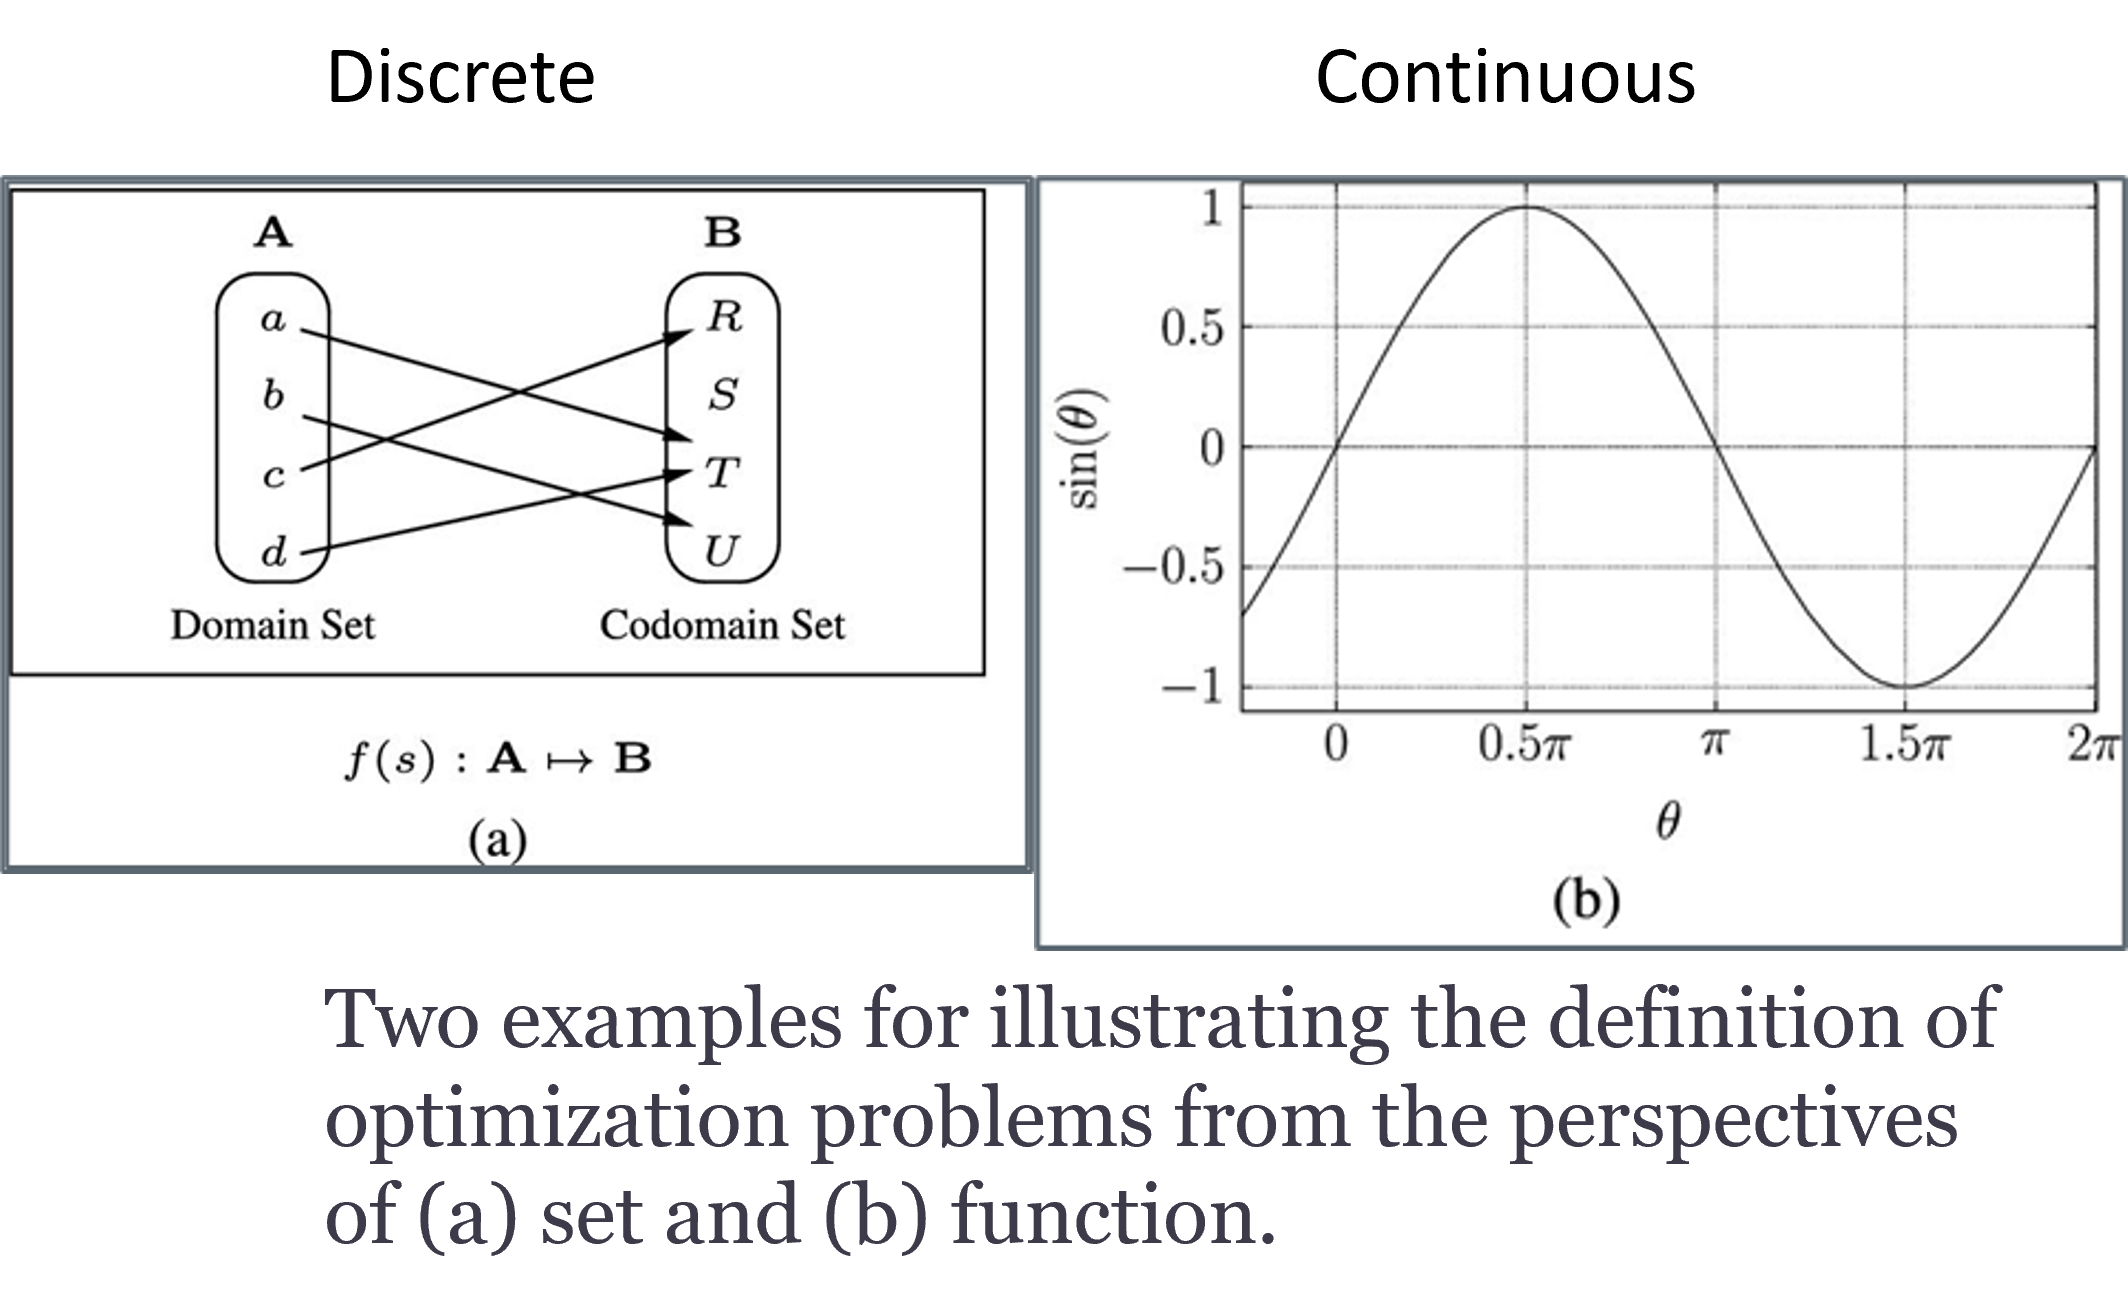
\includegraphics[keepaspectratio]{Pictures/ContDisc.png}}

}

\caption{Discrete vs Continuous}

\end{figure}%

\subsection{Discrete}\label{discrete}

\begin{itemize}
\tightlist
\item
  Domain: The set of all possible input values for a function.
\item
  Codomain: The set of all potential output values that the function can
  map to.
\item
  An objective function is a function that is being optimized (maximized
  or minimized) in a given problem. It takes an input from the domain
  and produces an output in the codomain.
\item
  Given two sets \(A\) and \(B\), and an objective function \(f\), we
  can understand how the function maps elements from the domain \(A\) to
  the codomain \(B\).
\end{itemize}

\subsection{Continuous}\label{continuous}

\begin{itemize}
\tightlist
\item
  Shows the relationship between the angle θ and the value of sin⁡(θ) at
  specific points. This relationship arises from the trigonometric sine
  function, which describes a wave-like pattern that oscillates between
  -1 and 1.
\item
  θ represents the angle, typically in radians, and the values given (0,
  0.25\(\pi\), 0.50\(\pi\), etc.) are specific points along the unit
  circle.
\item
  sin(θ) represents the sine of the angle θ, which is the y-coordinate
  of the corresponding point on the unit circle.
\item
  The values provided in the table correspond to these properties of the
  sine function. The function gradually increases from 0 to 1, then
  decreases back to 0, then continues to -1, and finally returns to 0,
  completing one full cycle.
\end{itemize}

\bookmarksetup{startatroot}

\chapter{Combinatorial Optimization Problems
(COPs)}\label{combinatorial-optimization-problems-cops}

\begin{itemize}
\tightlist
\item
  The goal of COPs is to find the optimal solution from a finite set or
  a countably infinite set of solutions. The possible solutions of a COP
  are generally ``discrete'' or can be discretized.

  \begin{itemize}
  \tightlist
  \item
    Traveling Salesman Problem (TSP)
  \item
    The one-max
  \item
    0-1 knapsack problems
  \end{itemize}
\end{itemize}

\section{Traveling Salesman
Algorithm}\label{traveling-salesman-algorithm}

\[\min_{s \in \S_{\pi}} f(s) = \left[ \sum_{i=1}^{n-1} d\left(c_{\pi(i)}, c_{\pi(i+1)}\right) \right] + d\left(c_{\pi(n)}, c_{\pi(1)}\right)\]

Where \(c_{\pi} = \{ c_{\pi(1)}, c_{\pi(2)}, \dots, c_{\pi(n)} \}\),
that is, all permutations of the \(n\) cities.

\begin{figure}[H]

{\centering \pandocbounded{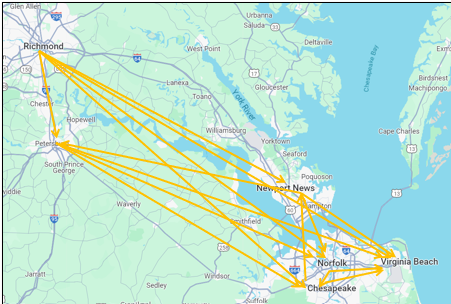
\includegraphics[keepaspectratio]{Pictures/GreedyMap.png}}

}

\caption{Greedy Map}

\end{figure}%

\subsection{Greedy TSP Solution}\label{greedy-tsp-solution}

\begin{itemize}
\item
  Start at Richmond. Find the nearest city. From Richmond, the nearest
  city is Petersburg (25 miles). Move to Petersburg.
\item
  From Petersburg, find the nearest unvisited city, which is Newport
  News (65 miles). Move to Newport News .
\item
  From Newport News, the nearest unvisited city is Norfolk (30 miles).
  Move to Norfolk.
\item
  From Norfolk, the nearest unvisited city is Chesapeake (10 miles).Move
  to Chesapeake.
\item
  From Chesapeake, the only unvisited city left is Virginia Beach (15
  miles). Move to Virginia Beach.
\item
  Finally, return to Richmond from Virginia Beach (100 miles).
\item
  Richmond -\textgreater{} Petersburg -\textgreater{} Newport News
  -\textgreater{} Norfolk -\textgreater{} Chesapeake -\textgreater{}
  Virginia Beach -\textgreater{} Richmond
\item
  Total distance traveled: = 25+65+30+10+15+100 = 245 miles
\end{itemize}

\begin{figure}[H]

{\centering \pandocbounded{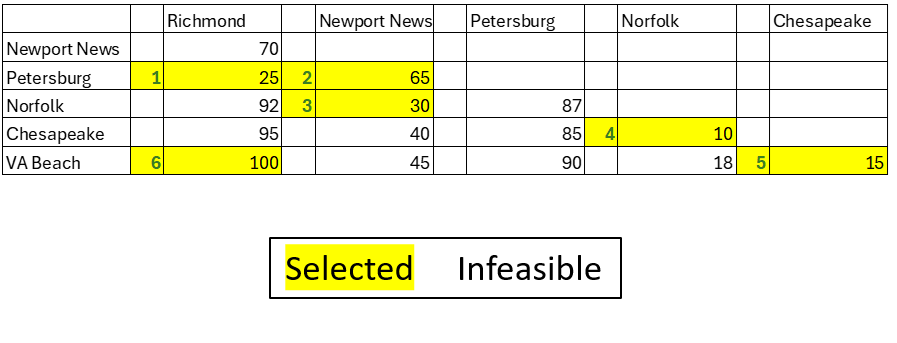
\includegraphics[keepaspectratio]{Pictures/tsp2.png}}

}

\caption{TSP Feasibility Map}

\end{figure}%

\bookmarksetup{startatroot}

\chapter{TSP Python Implementation}\label{tsp-python-implementation}

\bookmarksetup{startatroot}

\chapter{Dictionary vs Dictionary of
Dictionaries}\label{dictionary-vs-dictionary-of-dictionaries}

\begin{itemize}
\tightlist
\item
  A dictionary in Python is a built-in data structure that stores data
  in key-value pairs. It is unordered, mutable, and indexed by unique
  keys. The structure is enclosed within curly braces \{\}. Each key is
  associated with a value, and the two are separated by a colon :. Keys
  must be immutable types like strings, numbers, or tuples, while values
  can be of any data type, including other dictionaries.
\end{itemize}

\begin{Shaded}
\begin{Highlighting}[]
\NormalTok{my\_dict }\OperatorTok{=}\NormalTok{ \{}
     \StringTok{"key1"}\NormalTok{: }\StringTok{"value1"}\NormalTok{,}
     \StringTok{"key2"}\NormalTok{: }\StringTok{"value2"}\NormalTok{,}
     \StringTok{"key3"}\NormalTok{: }\StringTok{"value3"}
\NormalTok{\}}
\end{Highlighting}
\end{Shaded}

\begin{itemize}
\item
  A dictionary of dictionaries is a nested data structure in Python
  where the values of a dictionary are themselves dictionaries. It
  allows for organizing hierarchical or complex data in a structured
  way. This type of dictionary is especially useful for representing
  relationships, groupings, or matrices where each primary key maps to
  another dictionary of key-value pairs.
\item
  A distance matrix or distance map is helpful in implementing a TSP
  model in python can use the dictionary of dictionaries structure in
  python to implement. A distance map stores the distances between each
  pair of locations.

  \begin{itemize}
  \tightlist
  \item
    Outer Dictionary: Each key represents a city.
  \item
    Inner Dictionary: Contains distances to other cities from that city.
  \end{itemize}

  ::: \{.cell execution\_count=3\}
  \texttt{\{.python\ .cell-code\}\ \ \ distances\ =\ \{\ \ \ \ \ \ \ \textquotesingle{}City1\textquotesingle{}:\ \{\textquotesingle{}City2\textquotesingle{}:\ 5,\ \textquotesingle{}City3\textquotesingle{}:\ 10\},\ \ \ \ \ \ \ \textquotesingle{}City2\textquotesingle{}:\ \{\textquotesingle{}City1\textquotesingle{}:\ 5,\ \textquotesingle{}City3\textquotesingle{}:\ 8\},\ \ \ \ \ \ \ \textquotesingle{}City3\textquotesingle{}:\ \{\textquotesingle{}City1\textquotesingle{}:\ 10,\ \textquotesingle{}City2\textquotesingle{}:\ 8\}\ \ \ \}}
  :::
\item
  Each key (e.g., `City1') represents a location. Each inner dictionary
  provides distances to the other cities.
\end{itemize}

\begin{Shaded}
\begin{Highlighting}[]
\CommentTok{\# Define the cities and distances between them}
\NormalTok{cities }\OperatorTok{=}\NormalTok{ [}\StringTok{\textquotesingle{}Richmond\textquotesingle{}}\NormalTok{, }\StringTok{\textquotesingle{}Petersburg\textquotesingle{}}\NormalTok{, }\StringTok{\textquotesingle{}Chesapeake\textquotesingle{}}\NormalTok{, }\StringTok{\textquotesingle{}Norfolk\textquotesingle{}}\NormalTok{, }\StringTok{\textquotesingle{}Newport News\textquotesingle{}}\NormalTok{, }\StringTok{\textquotesingle{}Virginia Beach\textquotesingle{}}\NormalTok{]}

\CommentTok{\# Distances matrix (symmetric)}
\NormalTok{distances }\OperatorTok{=}\NormalTok{ \{}
    \StringTok{\textquotesingle{}Richmond\textquotesingle{}}\NormalTok{: \{}\StringTok{\textquotesingle{}Petersburg\textquotesingle{}}\NormalTok{: }\DecValTok{25}\NormalTok{, }\StringTok{\textquotesingle{}Chesapeake\textquotesingle{}}\NormalTok{: }\DecValTok{95}\NormalTok{, }\StringTok{\textquotesingle{}Norfolk\textquotesingle{}}\NormalTok{: }\DecValTok{92}\NormalTok{, }\StringTok{\textquotesingle{}Newport News\textquotesingle{}}\NormalTok{: }\DecValTok{70}\NormalTok{, }\StringTok{\textquotesingle{}Virginia Beach\textquotesingle{}}\NormalTok{: }\DecValTok{100}\NormalTok{\},}
    \StringTok{\textquotesingle{}Petersburg\textquotesingle{}}\NormalTok{: \{}\StringTok{\textquotesingle{}Richmond\textquotesingle{}}\NormalTok{: }\DecValTok{25}\NormalTok{, }\StringTok{\textquotesingle{}Chesapeake\textquotesingle{}}\NormalTok{: }\DecValTok{85}\NormalTok{, }\StringTok{\textquotesingle{}Norfolk\textquotesingle{}}\NormalTok{: }\DecValTok{87}\NormalTok{, }\StringTok{\textquotesingle{}Newport News\textquotesingle{}}\NormalTok{: }\DecValTok{65}\NormalTok{, }\StringTok{\textquotesingle{}Virginia Beach\textquotesingle{}}\NormalTok{: }\DecValTok{90}\NormalTok{\},}
    \StringTok{\textquotesingle{}Chesapeake\textquotesingle{}}\NormalTok{: \{}\StringTok{\textquotesingle{}Richmond\textquotesingle{}}\NormalTok{: }\DecValTok{95}\NormalTok{, }\StringTok{\textquotesingle{}Petersburg\textquotesingle{}}\NormalTok{: }\DecValTok{85}\NormalTok{, }\StringTok{\textquotesingle{}Norfolk\textquotesingle{}}\NormalTok{: }\DecValTok{10}\NormalTok{, }\StringTok{\textquotesingle{}Newport News\textquotesingle{}}\NormalTok{: }\DecValTok{40}\NormalTok{, }\StringTok{\textquotesingle{}Virginia Beach\textquotesingle{}}\NormalTok{: }\DecValTok{15}\NormalTok{\},}
    \StringTok{\textquotesingle{}Norfolk\textquotesingle{}}\NormalTok{: \{}\StringTok{\textquotesingle{}Richmond\textquotesingle{}}\NormalTok{: }\DecValTok{92}\NormalTok{, }\StringTok{\textquotesingle{}Petersburg\textquotesingle{}}\NormalTok{: }\DecValTok{87}\NormalTok{, }\StringTok{\textquotesingle{}Chesapeake\textquotesingle{}}\NormalTok{: }\DecValTok{10}\NormalTok{, }\StringTok{\textquotesingle{}Newport News\textquotesingle{}}\NormalTok{: }\DecValTok{30}\NormalTok{, }\StringTok{\textquotesingle{}Virginia Beach\textquotesingle{}}\NormalTok{: }\DecValTok{18}\NormalTok{\},}
    \StringTok{\textquotesingle{}Newport News\textquotesingle{}}\NormalTok{: \{}\StringTok{\textquotesingle{}Richmond\textquotesingle{}}\NormalTok{: }\DecValTok{70}\NormalTok{, }\StringTok{\textquotesingle{}Petersburg\textquotesingle{}}\NormalTok{: }\DecValTok{65}\NormalTok{, }\StringTok{\textquotesingle{}Chesapeake\textquotesingle{}}\NormalTok{: }\DecValTok{40}\NormalTok{, }\StringTok{\textquotesingle{}Norfolk\textquotesingle{}}\NormalTok{: }\DecValTok{30}\NormalTok{, }\StringTok{\textquotesingle{}Virginia Beach\textquotesingle{}}\NormalTok{: }\DecValTok{45}\NormalTok{\},}
    \StringTok{\textquotesingle{}Virginia Beach\textquotesingle{}}\NormalTok{: \{}\StringTok{\textquotesingle{}Richmond\textquotesingle{}}\NormalTok{: }\DecValTok{100}\NormalTok{, }\StringTok{\textquotesingle{}Petersburg\textquotesingle{}}\NormalTok{: }\DecValTok{90}\NormalTok{, }\StringTok{\textquotesingle{}Chesapeake\textquotesingle{}}\NormalTok{: }\DecValTok{15}\NormalTok{, }\StringTok{\textquotesingle{}Norfolk\textquotesingle{}}\NormalTok{: }\DecValTok{18}\NormalTok{, }\StringTok{\textquotesingle{}Newport News\textquotesingle{}}\NormalTok{: }\DecValTok{45}\NormalTok{\}}
\NormalTok{\}}

\NormalTok{start\_city }\OperatorTok{=} \StringTok{\textquotesingle{}Richmond\textquotesingle{}}

\CommentTok{\# Function to find the nearest neighbor}
\KeywordTok{def}\NormalTok{ find\_nearest\_neighbor(current\_city, unvisited):}
\NormalTok{    nearest\_city }\OperatorTok{=} \VariableTok{None}
\NormalTok{    min\_distance }\OperatorTok{=} \BuiltInTok{float}\NormalTok{(}\StringTok{\textquotesingle{}inf\textquotesingle{}}\NormalTok{)}
    \ControlFlowTok{for}\NormalTok{ city }\KeywordTok{in}\NormalTok{ unvisited:}
        \ControlFlowTok{if}\NormalTok{ distances[current\_city][city] }\OperatorTok{\textless{}}\NormalTok{ min\_distance:}
\NormalTok{            min\_distance }\OperatorTok{=}\NormalTok{ distances[current\_city][city]}
\NormalTok{            nearest\_city }\OperatorTok{=}\NormalTok{ city}
    \ControlFlowTok{return}\NormalTok{ nearest\_city, min\_distance}

\CommentTok{\# Nearest Neighbor algorithm implementation}
\KeywordTok{def}\NormalTok{ nearest\_neighbor\_tsp(start\_city):}
\NormalTok{    unvisited }\OperatorTok{=}\NormalTok{ cities.copy()}
\NormalTok{    unvisited.remove(start\_city)}
\NormalTok{    current\_city }\OperatorTok{=}\NormalTok{ start\_city}
\NormalTok{    route }\OperatorTok{=}\NormalTok{ [start\_city]}
\NormalTok{    total\_distance }\OperatorTok{=} \DecValTok{0}
    
    \ControlFlowTok{while}\NormalTok{ unvisited:}
\NormalTok{        next\_city, distance }\OperatorTok{=}\NormalTok{ find\_nearest\_neighbor(current\_city, unvisited)}
\NormalTok{        route.append(next\_city)}
\NormalTok{        total\_distance }\OperatorTok{+=}\NormalTok{ distance}
\NormalTok{        current\_city }\OperatorTok{=}\NormalTok{ next\_city}
\NormalTok{        unvisited.remove(current\_city)}
    
    \CommentTok{\# Return to the starting city}
\NormalTok{    total\_distance }\OperatorTok{+=}\NormalTok{ distances[current\_city][start\_city]}
\NormalTok{    route.append(start\_city)}
    
    \ControlFlowTok{return}\NormalTok{ route, total\_distance}

\CommentTok{\# Running the algorithm starting from Richmond}
\NormalTok{route, total\_distance }\OperatorTok{=}\NormalTok{ nearest\_neighbor\_tsp(start\_city)}

\CommentTok{\# Output the result}
\BuiltInTok{print}\NormalTok{(}\StringTok{"Optimal route using Nearest Neighbor:"}\NormalTok{, }\StringTok{" {-}\textgreater{} "}\NormalTok{.join(route))}
\BuiltInTok{print}\NormalTok{(}\StringTok{"Total distance traveled:"}\NormalTok{, total\_distance, }\StringTok{"miles"}\NormalTok{)}
\end{Highlighting}
\end{Shaded}

\begin{verbatim}
Optimal route using Nearest Neighbor: Richmond -> Petersburg -> Newport News -> Norfolk -> Chesapeake -> Virginia Beach -> Richmond
Total distance traveled: 245 miles
\end{verbatim}

\bookmarksetup{startatroot}

\chapter{Using AI}\label{using-ai-2}

\begin{itemize}
\tightlist
\item
  Use the following prompt on a generative AI, like chatGPT, to learn
  more about the topics covered.
\item
  Greedy Decisions: Think of a real-world example where you made a
  ``greedy'' choice (choosing the option that seemed best at the
  moment). Did it lead to the best possible outcome? Why or why not?
\item
  Optimization Problems: Explain the difference between discrete and
  continuous optimization problems. Give a real-world example of each
  type.
\item
  Coin Change Problem: Implement the greedy\_coin\_change function from
  the slides. Then, modify it to handle cases where the denominations do
  not lead to an optimal solution. Explain the changes made.
\item
  Nearest Neighbor TSP: Given a distance matrix for a Traveling Salesman
  Problem (TSP), write Python code using the greedy nearest neighbor
  approach. Compare its solution to the optimal path for the same
  problem.
\item
  Greedy Limitations: Discuss a problem where a greedy algorithm does
  not guarantee the optimal solution. How could this limitation be
  addressed (e.g., using dynamic programming or exhaustive search)?
\item
  Practical Scenarios: Discuss a real-world system (e.g., ride-sharing,
  network routing, or resource allocation) where greedy algorithms are
  used. What trade-offs do they involve?
\item
  Designing a Greedy Algorithm: Create your own optimization problem and
  solve it using a greedy algorithm. Explain your reasoning and solution
  step-by-step.
\end{itemize}

\bookmarksetup{startatroot}

\chapter{Conclusions}\label{conclusions-1}

\begin{itemize}
\tightlist
\item
  While greedy algorithms can provide optimal solutions for certain
  problems (e.g., fractional knapsack), they don't always guarantee an
  optimal result for all problems. Understanding when to use them is
  key.
\item
  Greedy algorithms guarantee an optimal solution for problems that
  exhibit the greedy choice property. However, the Greedy Algorithm may
  not always yield the optimal solution. Greedy works well for certain
  problems like the Coin Change Problem with standard denominations.
\item
  Greedy algorithms can be faster and more efficient in terms of time
  complexity compared to other approaches (like dynamic programming or
  exhaustive search), especially when the problem size is large.
\item
  The approach is simple and efficient, making it ideal for many
  practical scenarios. Greedy algorithms typically use less memory
  because they do not need to store all possible solutions or
  intermediate results, unlike dynamic programming or exhaustive search
  methods.
\end{itemize}

\bookmarksetup{startatroot}

\chapter{Benchmark Optimization
Problems}\label{benchmark-optimization-problems}

\bookmarksetup{startatroot}

\chapter{Benchmark Problems:
Overview}\label{benchmark-problems-overview}

\begin{itemize}
\tightlist
\item
  OneMax Problem: The OneMax problem is widely used as a benchmark in
  evolutionary algorithms to test how well algorithms can evolve a
  binary string towards an optimal solution (a string of all 1s). It is
  simple and useful for evaluating basic evolutionary or heuristic
  search methods. Knapsack Problem: The Knapsack problem is another
  classic benchmark problem in optimization, particularly for
  combinatorial algorithms. Variants such as the 0/1 Knapsack and
  Fractional Knapsack are commonly used to evaluate algorithms like
  dynamic programming, greedy algorithms, and evolutionary methods.
\item
  Ackley Function: The Ackley function is a well-known continuous
  optimization benchmark problem. It is often used to test optimization
  algorithms' ability to handle multi-modal functions with many local
  minima. Algorithms like simulated annealing and genetic algorithms are
  frequently evaluated using this function.
\item
  Schaffer Min-Min Problem: he Schaffer Min-Min is a well-known
  benchmark in multi-objective optimization. It provides a simple yet
  effective test case for algorithms that need to identify
  Pareto-optimal solutions in multi-objective spaces.
\item
  These benchmark problems are critical for testing and comparing the
  performance of optimization algorithms, especially in research and
  development of new heuristic methods.
\end{itemize}

\bookmarksetup{startatroot}

\chapter{Discrete Optimization
Problems}\label{discrete-optimization-problems}

\section{OneMax Problem}\label{onemax-problem}

\begin{itemize}
\item
  In evolutionary algorithms, the OneMax problem serves as a simple test
  problem where the goal is to evolve a population of binary strings
  towards the optimal solution (a string of all 1s). The fitness
  function is used to evaluate the quality of each candidate solution in
  the population.
\item
  Fitness Function: Imagine life had a personal `fitness function' just
  for you. What variables would you include in it, and how would you
  weigh them?
\end{itemize}

\subsection{One Max Formula}\label{one-max-formula}

\begin{itemize}
\tightlist
\item
  Binary String: A binary string is generated using NumPy's randint
  function, which creates a list of 0s and 1s. It can be any positive
  integer.
\item
  Fitness Function: The one\_max function calculates the ``fitness'' of
  the binary string, which is simply the sum of all 1s in the string.
  This is the value that needs to be maximized.
\item
  Example Run: If the generated binary string is {[}1, 0, 1, 1, 0, 1, 0,
  1, 1, 0{]}, the fitness would be 6, since there are six 1s in the
  string.
\item
  The objective is to maximize the number of 1s in a binary string.
\end{itemize}

\[\max_{s \in A} f(s) = \sum_{i=1}^{n} s_i, \quad \text{subject to} \ s_i \in \{0, 1\}.\]

\subsection{Optimal Solution OneMax}\label{optimal-solution-onemax}

\begin{itemize}
\tightlist
\item
  The optimal solution of this problem is that all the subsolutions
  assume the value 1; i.e., \(s_i=1\) for all \(i\). For instance, the
  optimal solution for \(n=4\) is \(s^*=(1111)\) and the objective value
  of a possible solution \(s^*=(0111)\) can be easily calculated as the
  count of the number of ones in the solution \(s\) as the objective
  function if \(f(s) = f(0111) = 0+1+1+1 = 3\)
\end{itemize}

\subsection{OneMax Pseudocode}\label{onemax-pseudocode}

\begin{Shaded}
\begin{Highlighting}[]
\NormalTok{Pseudocode:}


\NormalTok{FUNCTION one\_max(binary\_string):}
\NormalTok{\# Calculate the fitness as the sum of 1s in the binary string}
\NormalTok{    RETURN sum(binary\_string)}

\NormalTok{\# Example usage}
\NormalTok{SET n = 10  \# Length of the binary string}

\NormalTok{\# Generate a random binary string of length n}
\NormalTok{SET binary\_string = generate a random list of 0s and 1s of size n}

\NormalTok{\# Calculate the fitness}
\NormalTok{SET fitness = one\_max(binary\_string)}

\NormalTok{\# Print the binary string and its fitness}
\NormalTok{PRINT "Binary string:", binary\_string}
\NormalTok{PRINT "Fitness (number of 1s):", fitness}
\end{Highlighting}
\end{Shaded}

\subsection{OneMax Python
Implementation}\label{onemax-python-implementation}

\begin{Shaded}
\begin{Highlighting}[]
\ImportTok{import}\NormalTok{ numpy }\ImportTok{as}\NormalTok{ np}
\ImportTok{import}\NormalTok{ matplotlib.pyplot }\ImportTok{as}\NormalTok{ plt}
\ImportTok{import}\NormalTok{ seaborn }\ImportTok{as}\NormalTok{ sns}

\KeywordTok{def}\NormalTok{ one\_max(binary\_string):}
    \ControlFlowTok{return} \BuiltInTok{sum}\NormalTok{(binary\_string)}

\CommentTok{\# Example usage: \# Length of the binary string}
\NormalTok{n }\OperatorTok{=} \DecValTok{10}

\CommentTok{\# Generate a random binary string of length n}
\NormalTok{binary\_string }\OperatorTok{=}\NormalTok{ np.random.randint(}\DecValTok{0}\NormalTok{, }\DecValTok{2}\NormalTok{, size}\OperatorTok{=}\NormalTok{n).tolist()}

\CommentTok{\# Calculate the fitness}
\NormalTok{fitness }\OperatorTok{=}\NormalTok{ one\_max(binary\_string)}

\BuiltInTok{print}\NormalTok{(}\SpecialStringTok{f"Binary string: }\SpecialCharTok{\{}\NormalTok{binary\_string}\SpecialCharTok{\}}\SpecialStringTok{"}\NormalTok{)}
\BuiltInTok{print}\NormalTok{(}\SpecialStringTok{f"Fitness (number of 1s): }\SpecialCharTok{\{}\NormalTok{fitness}\SpecialCharTok{\}}\SpecialStringTok{"}\NormalTok{)}


\NormalTok{iterations }\OperatorTok{=} \DecValTok{20}
\NormalTok{fitness\_over\_time }\OperatorTok{=}\NormalTok{ [np.random.randint(}\DecValTok{0}\NormalTok{, n }\OperatorTok{+} \DecValTok{1}\NormalTok{) }\ControlFlowTok{for}\NormalTok{ \_ }\KeywordTok{in} \BuiltInTok{range}\NormalTok{(iterations)]  }\CommentTok{\# Random example of fitness change}

\CommentTok{\# Line plot of fitness over iterations}
\NormalTok{plt.figure(figsize}\OperatorTok{=}\NormalTok{(}\DecValTok{10}\NormalTok{, }\DecValTok{4}\NormalTok{))}
\NormalTok{plt.plot(}\BuiltInTok{range}\NormalTok{(iterations), fitness\_over\_time, marker}\OperatorTok{=}\StringTok{\textquotesingle{}o\textquotesingle{}}\NormalTok{, color}\OperatorTok{=}\StringTok{\textquotesingle{}green\textquotesingle{}}\NormalTok{, linestyle}\OperatorTok{=}\StringTok{\textquotesingle{}{-}\textquotesingle{}}\NormalTok{, linewidth}\OperatorTok{=}\DecValTok{2}\NormalTok{)}
\NormalTok{plt.fill\_between(}\BuiltInTok{range}\NormalTok{(iterations), fitness\_over\_time, color}\OperatorTok{=}\StringTok{\textquotesingle{}lightgreen\textquotesingle{}}\NormalTok{, alpha}\OperatorTok{=}\FloatTok{0.4}\NormalTok{)}
\NormalTok{plt.title(}\SpecialStringTok{f"Fitness Evolution Over Time"}\NormalTok{)}
\NormalTok{plt.xlabel(}\StringTok{"Iteration"}\NormalTok{)}
\NormalTok{plt.ylabel(}\StringTok{"Fitness (number of 1s)"}\NormalTok{)}
\NormalTok{plt.xticks(np.arange(}\DecValTok{0}\NormalTok{, iterations, step}\OperatorTok{=}\DecValTok{1}\NormalTok{))  }\CommentTok{\# Show whole numbers on the x{-}axis}

\NormalTok{plt.grid(}\VariableTok{True}\NormalTok{)}
\NormalTok{plt.show()}
\end{Highlighting}
\end{Shaded}

\begin{verbatim}
Binary string: [1, 1, 0, 0, 0, 0, 0, 1, 1, 0]
Fitness (number of 1s): 4
\end{verbatim}

\pandocbounded{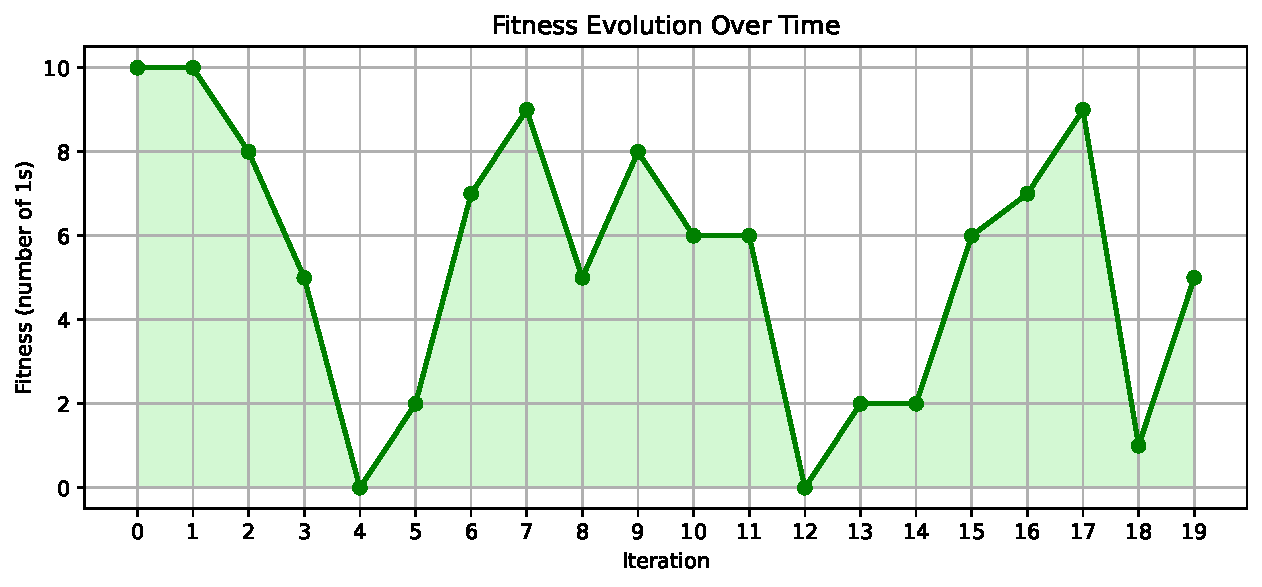
\includegraphics[keepaspectratio]{benchmark_files/figure-pdf/cell-2-output-2.pdf}}

\begin{itemize}
\tightlist
\item
  The plot above tracks how fitness improves or changes across
  iterations in an optimization algorithm, giving insight into the
  convergence of the algorithm.
\end{itemize}

\subsection{Comparing OneMax Problem to Greedy
Algorithm}\label{comparing-onemax-problem-to-greedy-algorithm}

\begin{itemize}
\tightlist
\item
  If a greedy search algorithm is used and is allowed to randomly add
  one to or subtract one from the current solution \(s\) to create the
  next possible solution \(v\) for solving the one-max problem, that is,
  it is allowed to move one and only one step to either the left or the
  right of the current solution in the landscape of the solution space.
\item
  Without knowledge of the landscape of the solution space, the search
  process will easily get stuck in the peaks of this solution space.
\item
  Hence, most researchers prefer using the one-max problem as an example
  because it is easy to implement and also because it can be used to
  prove if a new concept for a search algorithm is correct.
\end{itemize}

\pandocbounded{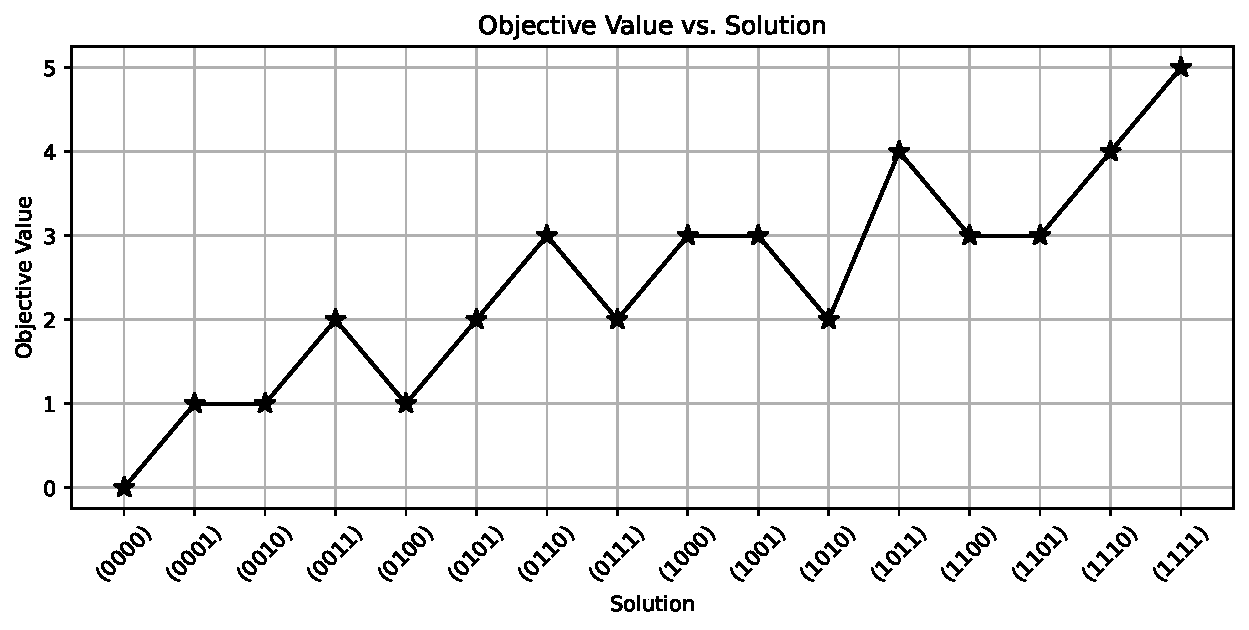
\includegraphics[keepaspectratio]{benchmark_files/figure-pdf/cell-3-output-1.pdf}}

\section{The Knapsack Problem}\label{the-knapsack-problem}

\begin{itemize}
\item
  The Knapsack Problem is a classic NP-complete optimization problem,
  where you are given a set of items, each with a weight and a value.
\item
  The goal is to determine the number of each item to include in a
  collection so that the total weight is less than or equal to a given
  limit and the total value is as large as possible.
\item
  Types of Knapsack Problems:

  \begin{itemize}
  \tightlist
  \item
    0/1 Knapsack Problem:

    \begin{itemize}
    \tightlist
    \item
      Each item can be included (1) or excluded (0) in the knapsack.
    \item
      You cannot break items into smaller parts.
      \(\max_{s \in A} f(s) = \sum_{i=1}^{n} s_i v_i, \quad \text{subject to} \quad w(s) = \sum_{i=1}^{n} s_i w_i \leq W, \quad s_i \in \{0, 1\}\)
      Where \(v_i\) is the value associated with \(s_1\) and \(w_i\) is
      the weight associated with \(s_i\)
    \end{itemize}
  \item
    Fractional Knapsack Problem:

    \begin{itemize}
    \tightlist
    \item
      You can break items into smaller parts and include fractions of
      them in the knapsack.
    \item
      Ratio = \(\frac{v_i}{w_i}\), where \(v_i\) is the value of item
      \(i\), and \(w_i\) is the weight of item \(i\).
    \end{itemize}
  \end{itemize}
\end{itemize}

\subsection{NP Complete}\label{np-complete}

\begin{itemize}
\tightlist
\item
  NP (Nondeterministic Polynomial Time): A problem is in NP if a
  solution can be verified in polynomial time by a deterministic
  algorithm. In other words, given a solution, it is possible to check
  if it is correct relatively quickly (in polynomial time). However,
  finding the solution itself might take much longer (potentially
  exponential time) unless the problem can also be solved in polynomial
  time.
\item
  NP-complete refers to a class of problems in computational complexity
  theory that are both NP (nondeterministic polynomial time) and every
  problem in NP can be reduced to it in polynomial time
\item
  NP-hard problems are optimization or decision problems that are at
  least as difficult to solve as the hardest problems in NP
  (nondeterministic polynomial time).

  \begin{itemize}
  \tightlist
  \item
    Unlike NP-complete problems, NP-hard problems do not have to be
    verifiable in polynomial time. This means that while it may be
    incredibly hard to find an optimal solution, even verifying a
    proposed solution might take more than polynomial time.
  \item
    Essentially, NP-hard problems are hard to solve optimally, and their
    complexity often prevents efficient algorithms from finding or
    checking solutions within a reasonable time frame.
  \item
    NP-hard problems are broader and potentially harder than NP-complete
    problems because they can include problems that aren't even in NP.
    They may not have a polynomial-time verification process.
  \end{itemize}
\end{itemize}

\subsection{Key Characteristics of NP-complete
Problems}\label{key-characteristics-of-np-complete-problems}

\begin{itemize}
\item
  Difficult to solve: No known algorithms can solve NP-complete problems
  efficiently (in polynomial time) for all instances.
\item
  Verification in polynomial time: If someone provides a solution, it
  can be verified quickly. Equivalence to other NP-complete problems: If
  one NP-complete problem can be solved in polynomial time, all
  NP-complete problems can be solved in polynomial time.
\item
  Knapsack Problem: The 0/1 knapsack problem is NP-complete. Finding the
  optimal solution is hard, but verifying if a solution meets the
  constraints and maximizes value can be done in polynomial time.
\item
  The Fractional knapsack problem is not NP-complete and can be solved
  in polynomial time using a greedy algorithm.
\item
  The Travelling Salesman is a NP-hard problem.
\end{itemize}

\subsection{Example Fractional Knapsack
Problem}\label{example-fractional-knapsack-problem}

\begin{itemize}
\item
  Knapsack Capacity: 15 kg

  \begin{itemize}
  \tightlist
  \item
    Items Available:

    \begin{itemize}
    \tightlist
    \item
      Item 1: Value = 10, Weight = 5 kg
    \item
      Item 2: Value = 40, Weight = 10 kg
    \item
      Item 3: Value = 30, Weight = 15 kg
    \end{itemize}
  \end{itemize}
\item
  Objective: Maximize the total value without exceeding 15 kg.
\item
  The greedy algorithm works well by prioritizing items with the highest
  value-to-weight ratio.
\item
  0/1 Knapsack Problem requires more complex algorithms like dynamic
  programming to find the optimal solution over the Fractional Knapsack
  Problem
\end{itemize}

\subsection{Greedy Algorithm for Fractional
Knapsack}\label{greedy-algorithm-for-fractional-knapsack}

\begin{itemize}
\tightlist
\item
  Step 1: Calculate Value-to-Weight Ratio:

  \begin{itemize}
  \tightlist
  \item
    Item 1: 10/5=2
  \item
    Item 2: 40/10=4
  \item
    Item 3: 30/15=2
  \end{itemize}
\item
  Step 2: Sort Items by Ratio (Descending): Item 2, Item 1, Item 3

  \begin{itemize}
  \tightlist
  \item
    Step 3: Fill the Knapsack:
  \item
    Take Item 2 (10 kg, Value = 40).
  \item
    Take as much of Item 1 as possible (5 kg, Value = 10).
  \end{itemize}
\item
  Results: Total Weight = 15 kg, Total Value = 50.
\end{itemize}

\section{Binary to Decimal (B2D) Problem:
B2D-1}\label{binary-to-decimal-b2d-problem-b2d-1}

\begin{itemize}
\tightlist
\item
  The binary to decimal model is often used in optimization problems,
  particularly in the context of genetic algorithms and heuristic
  methods.
\item
  With a minor modification, the solution space of the one-max problem
  can be simplified as the solution space of another optimization
  problem.
\item
  The model uses binary strings to represent numbers. Each string
  represents a decimal number when interpreted in binary form.
\item
  The B2D-1 problem is to maximize the value of the objective function
  of a binary string.
\end{itemize}

\subsection{Characteristics and Visualization of
B2D-1}\label{characteristics-and-visualization-of-b2d-1}

\begin{itemize}
\tightlist
\item
  These two examples are possible landscapes to the B2D problem.
\item
  The first chart to the left implies that there are only two possible
  next states (candidate solutions) that can be generated from the
  current solution except for solutions (0000) and (1111), which can
  only be moved to the right and to the left, respectively.
\item
  If another search algorithm can generate a new candidate solution by
  randomly inverting (flipping) one of the subsolutions of the current
  solution, the number of possible states of the new candidate solution
  will be \(n\), where \(n\) is the number of subsolutions.
\end{itemize}

\begin{figure}[H]

{\centering \pandocbounded{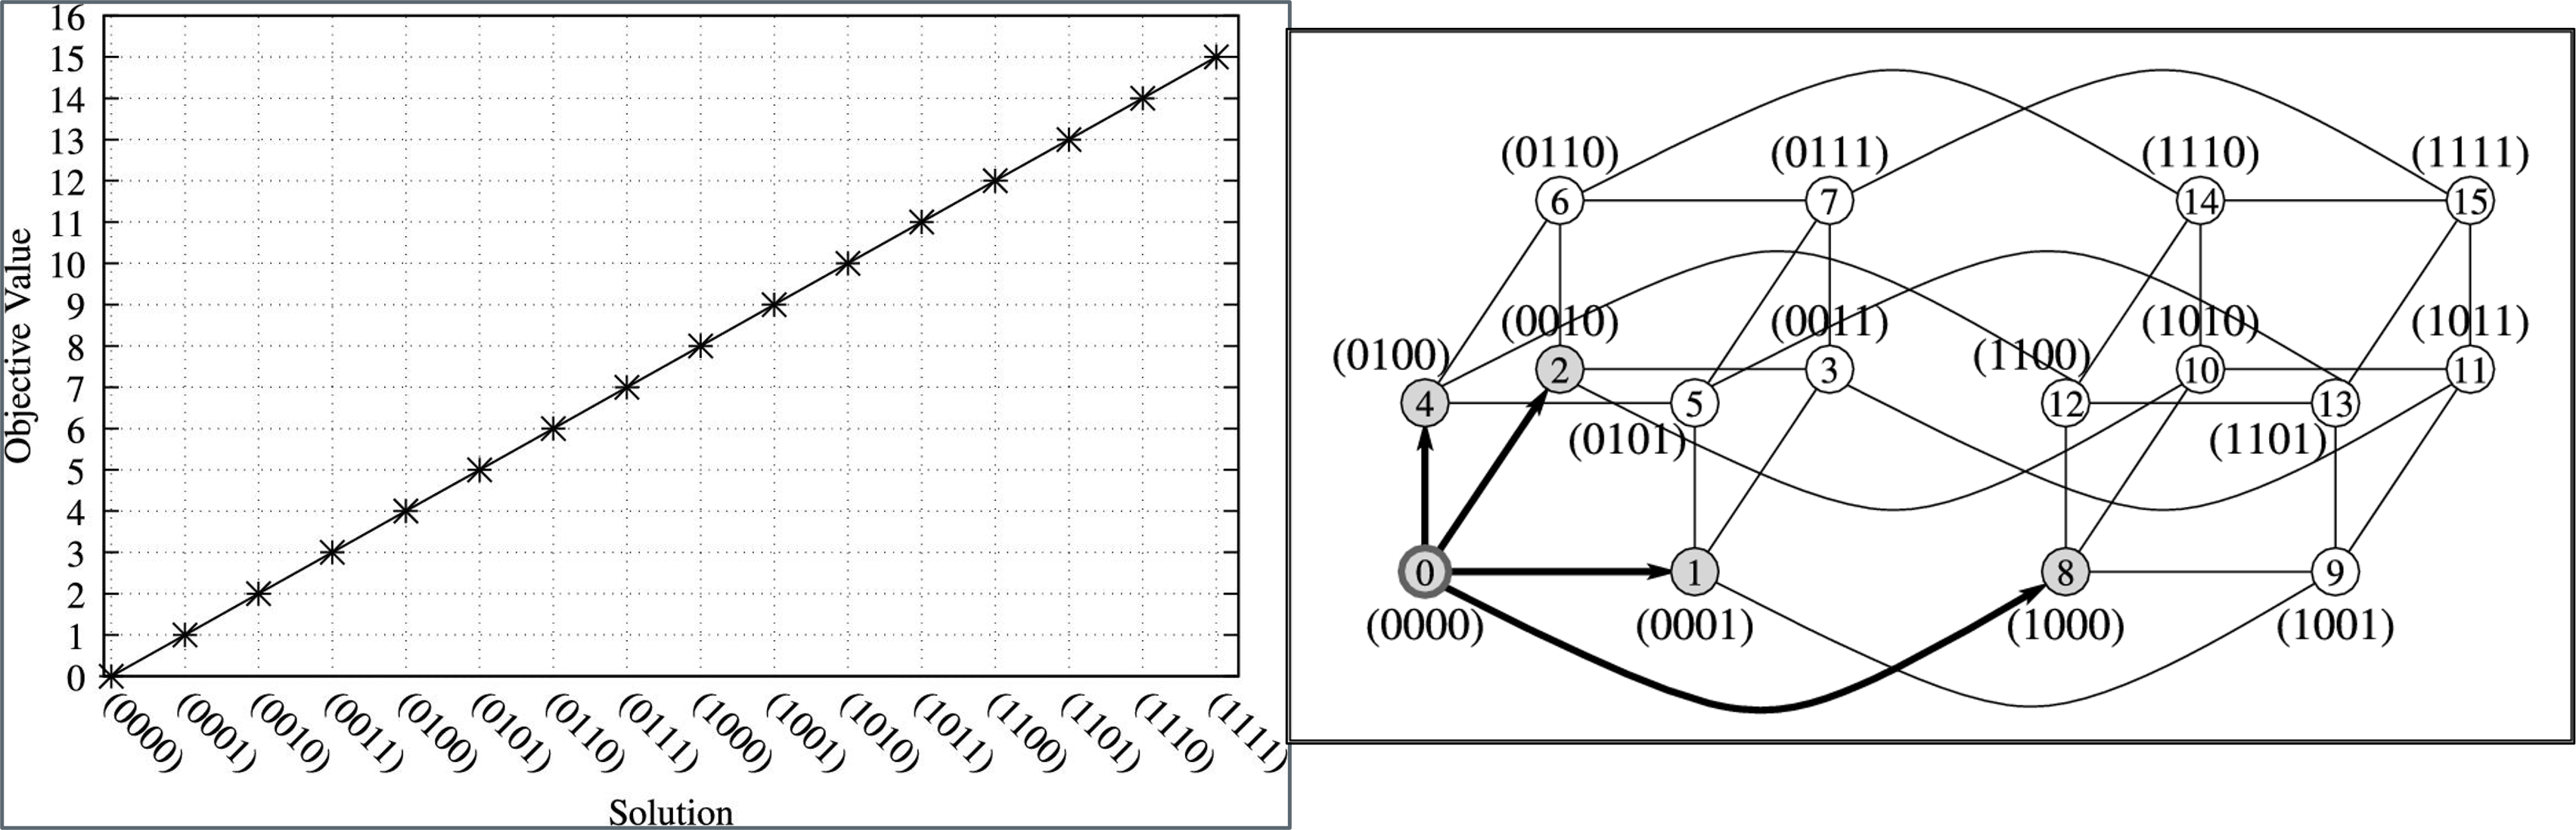
\includegraphics[keepaspectratio]{Pictures/OneMax.png}}

}

\caption{OneMax}

\end{figure}%

\section{B2D with Deception: B2D-2}\label{b2d-with-deception-b2d-2}

\begin{itemize}
\tightlist
\item
  B2D deception problems mislead optimization algorithms away from
  finding the global optimum by presenting local optima that seem
  promising but are actually suboptimal.
\item
  Used to test whether a search algorithm is capable of escaping local
  optima or not.
\item
  Deception problems highlight the necessity of exploration in heuristic
  algorithms, such as introducing diversity through mutation or
  crossover in genetic algorithms. If the algorithm becomes too greedy
  and focuses only on local fitness improvements (exploitation), it may
  get stuck at deceptive local optima.
\end{itemize}

\bookmarksetup{startatroot}

\chapter{Continuous Optimization
Problems}\label{continuous-optimization-problems}

\begin{itemize}
\tightlist
\item
  Unlike the COP, the possible solutions for a continuous optimization
  problem are typically ``uncountably infinite.'' This means that the
  number of solutions in the solution space is tantamount to the number
  of real values in the given space, that is, infinite.

  \begin{itemize}
  \tightlist
  \item
    Single-objective optimization problem (SOP)
  \item
    The Ackley optimization problem
  \end{itemize}
\item
  Multi-objective optimization problem (MOP)

  \begin{itemize}
  \tightlist
  \item
    The Schaffer Min-Min Global Optimization Problem
  \end{itemize}
\end{itemize}

\section{Single-objective Optimization Problem
(SOP)}\label{single-objective-optimization-problem-sop}

\begin{itemize}
\tightlist
\item
  A single-objective optimization problem involves finding the best
  solution from a set of feasible solutions based on a single objective
  function. The goal is to either maximize or minimize this objective
  function.
\end{itemize}

\[\underset{s \in \mathbb{R}^n}{\text{opt}} f(s), \quad \text{subject to } \, c_i(s) \odot b_i, \quad i = 1, 2, \ldots, m,\]

\begin{itemize}
\tightlist
\item
  where

  \begin{itemize}
  \tightlist
  \item
    \({R}^n\) and \({R}\) are the domain and codomain, respectively,
  \item
    \(f(s) {R}^n\) and \({R}\) is the objective function to be
    optimized,
  \item
    \(c_i(s): {R}^n\) and \({R}\odot b_i, \quad i = 1, 2, \ldots, m,\)
    are the constraints,
  \item
    and \(opt\) and \(\odot\) are as given in Definition 1 as \textless,
    \textgreater, =, ⩽, or ⩾.
  \end{itemize}
\end{itemize}

\subsection{Ackley Function: A Single Optimization
Problem}\label{ackley-function-a-single-optimization-problem}

\begin{itemize}
\tightlist
\item
  The Ackley Function is a widely used benchmark function for testing
  optimization algorithms. It is characterized by its multi-modal nature
  with a nearly flat outer region and a large hole at the center.
\item
  Applications

  \begin{itemize}
  \tightlist
  \item
    Used as a standard test case in evaluating the performance of
    optimization algorithms like genetic algorithms, simulated
    annealing, and particle swarm optimization.
  \item
    Relevant in fields such as machine learning, control systems, and
    operations research.
  \end{itemize}
\item
  Limitations

  \begin{itemize}
  \tightlist
  \item
    The function's large search space and numerous local minima make it
    difficult for algorithms to converge to the global minimum.
  \item
    Large importance of balancing exploration and exploitation in
    optimization strategies when dealing with the Ackley Function.
  \end{itemize}
\end{itemize}

\subsubsection{Explanation of Ackley Function(x,
y)}\label{explanation-of-ackley-functionx-y}

\begin{itemize}
\tightlist
\item
  Computes the value of the Ackley function given a point (x, y) in the
  search space.
\item
  The optimization algorithm optimizes the Ackley function to find the
  point where it reaches its minimum. It initializes a population of
  random solutions, evaluates their fitness (using the Ackley function),
  and iteratively improves them using an optimization method (like
  gradient descent or a genetic algorithm).
\item
  The best solution and corresponding function value (score) are
  returned as the result.
\end{itemize}

\subsubsection{Ackley function and B2D: Converting to
Decimal}\label{ackley-function-and-b2d-converting-to-decimal}

\begin{itemize}
\tightlist
\item
  The Ackley function uses the binary representation, where the binary
  strings need to be converted to decimal values (i.e., real numbers).
  In this case, the converted decimal values correspond to points in the
  continuous search space.
\item
  For example, a binary string like 1010 can be converted into a decimal
  value, which can then be used as input to the Ackley function. Binary
  String: 1010, where the binary number is 1010\_2.
\item
  Each position in the binary number represents a power of 2, starting
  from the right (least significant bit):
\item
  The rightmost bit (0) is \(2^0\),The next bit (1) is \(2^1\) ,The next
  bit (0) is \(2^2\),The leftmost bit (1) is \(2^3\).
\end{itemize}

\(1010_2= 0 ∗ 2^0+ 1 ∗ 2^1 +0 ∗ 2^2+1 ∗ 2^3\)
\(= 0 ∗ 1+ 1 ∗ 2 + 0 ∗ 4 + 1 ∗ 8\) \(=  0 + 2 + 0 + 8 = 10\) Thus, the
decimal equivalent of the binary string ``1010'' is 10. Use this value
as input for the Ackley function.

\subsubsection{Characteristics and Visualization of Ackley
Function}\label{characteristics-and-visualization-of-ackley-function}

\begin{itemize}
\tightlist
\item
  The Ackley function is evaluated in the hypercube.
\item
  The global optimum (minimum) of the Ackley function is 𝑓(𝑠\^{}∗)=0 is
  located at \(s^*=(0,0,…0)\).
\item
  This function has many local optima, which makes it hard for the
  search algorithm to find the global optimum.
\end{itemize}

\begin{figure}[H]

{\centering \pandocbounded{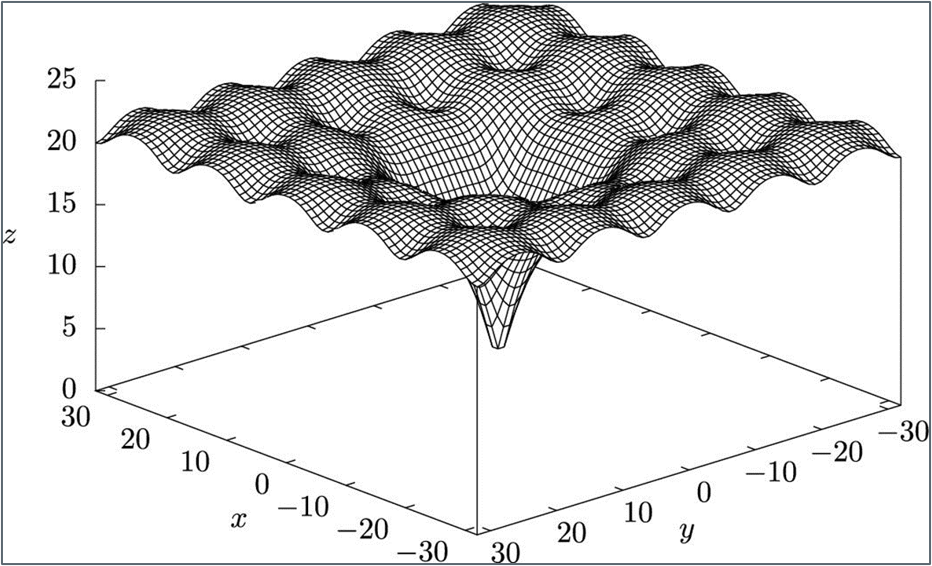
\includegraphics[keepaspectratio]{Pictures/GenericAckley.png}}

}

\caption{Ackley}

\end{figure}%

\subsubsection{Ackley Function Formula}\label{ackley-function-formula}

\[
\begin{array}{rl}
\min_{s \in \mathbb{R}^n} f(s) &= -20 \exp \left(-0.2 \sqrt{\frac{1}{n} \sum_{i=1}^n s_i^2} \right) \\
& \quad - \exp \left( \frac{1}{n} \sum_{i=1}^n \cos(2 \pi s_i) \right) + 20 + e, \\
\text{subject to} & \quad -30 \leq s_i \leq 30, \quad i = 1, 2, \dots, n.
\end{array}
\]

\subsubsection{Ackley Function:
Pseudocode}\label{ackley-function-pseudocode}

\begin{itemize}
\tightlist
\item
  The below example uses a random function to pull a point that we want
  to hit the local minima. You can imagine, this might not be the best
  way to do this.
\end{itemize}

\begin{Shaded}
\begin{Highlighting}[]
\NormalTok{PSEUDOCODE}
\NormalTok{FUNCTION Ackley(s):}
\NormalTok{    SET a = 20, b = 0.2, c = 2 * pi}
\NormalTok{    SET n = length of s}
\NormalTok{    COMPUTE sum\_sq\_term = sum of squares of all elements in s}
\NormalTok{    COMPUTE cos\_term = sum of cos(2 * pi * each element in s)}
    
\NormalTok{    COMPUTE term1 = {-}a * exp({-}b * sqrt(sum\_sq\_term / n))}
\NormalTok{    COMPUTE term2 = {-}exp(cos\_term / n)}
    
\NormalTok{    RETURN term1 + term2 + a + e}

\NormalTok{\# Main Execution}
\NormalTok{SET n = 2  \# Dimension of the Ackley function}

\NormalTok{\# Generate random vector s with elements between {-}30 and 30}
\NormalTok{SET s = random values in range [{-}30, 30] of length n}

\NormalTok{\# Compute the Ackley function result for the vector s}
\NormalTok{SET result = Ackley(s)}

\NormalTok{PRINT vector s}
\NormalTok{PRINT Ackley function result for vector s}
\end{Highlighting}
\end{Shaded}

\subsubsection{Ackley Function Python
Implementation}\label{ackley-function-python-implementation}

\begin{Shaded}
\begin{Highlighting}[]
\ImportTok{import}\NormalTok{ numpy }\ImportTok{as}\NormalTok{ np}
\ImportTok{import}\NormalTok{ matplotlib.pyplot }\ImportTok{as}\NormalTok{ plt}
\ImportTok{from}\NormalTok{ mpl\_toolkits.mplot3d }\ImportTok{import}\NormalTok{ Axes3D}

\NormalTok{np.random.seed(}\DecValTok{5042}\NormalTok{)}

\CommentTok{\# Ackley function implementation}
\KeywordTok{def}\NormalTok{ ackley(s):}
\NormalTok{    a, b, c }\OperatorTok{=} \DecValTok{20}\NormalTok{, }\FloatTok{0.2}\NormalTok{, }\DecValTok{2} \OperatorTok{*}\NormalTok{ np.pi}
\NormalTok{    n }\OperatorTok{=} \BuiltInTok{len}\NormalTok{(s)}
\NormalTok{    sum\_sq\_term }\OperatorTok{=}\NormalTok{ np.}\BuiltInTok{sum}\NormalTok{(s}\OperatorTok{**}\DecValTok{2}\NormalTok{)}
\NormalTok{    cos\_term }\OperatorTok{=}\NormalTok{ np.}\BuiltInTok{sum}\NormalTok{(np.cos(c }\OperatorTok{*}\NormalTok{ s))}
\NormalTok{    term1 }\OperatorTok{=} \OperatorTok{{-}}\NormalTok{a }\OperatorTok{*}\NormalTok{ np.exp(}\OperatorTok{{-}}\NormalTok{b }\OperatorTok{*}\NormalTok{ np.sqrt(sum\_sq\_term }\OperatorTok{/}\NormalTok{ n))}
\NormalTok{    term2 }\OperatorTok{=} \OperatorTok{{-}}\NormalTok{np.exp(cos\_term }\OperatorTok{/}\NormalTok{ n)}
    \ControlFlowTok{return}\NormalTok{ term1 }\OperatorTok{+}\NormalTok{ term2 }\OperatorTok{+}\NormalTok{ a }\OperatorTok{+}\NormalTok{ np.e}

\CommentTok{\# Example usage: }
\NormalTok{n }\OperatorTok{=} \DecValTok{2}  \CommentTok{\# Dimension }
\NormalTok{s }\OperatorTok{=}\NormalTok{ np.random.uniform(}\OperatorTok{{-}}\DecValTok{30}\NormalTok{, }\DecValTok{30}\NormalTok{, n)  }\CommentTok{\# Generate random s\_i values in the range [{-}30, 30]}

\NormalTok{result }\OperatorTok{=}\NormalTok{ ackley(s)  }\CommentTok{\# Evaluate the Ackley function}

\BuiltInTok{print}\NormalTok{(}\SpecialStringTok{f"Vector s: }\SpecialCharTok{\{}\NormalTok{s}\SpecialCharTok{\}}\SpecialStringTok{"}\NormalTok{)}
\BuiltInTok{print}\NormalTok{(}\SpecialStringTok{f"Ackley function result: }\SpecialCharTok{\{}\NormalTok{result}\SpecialCharTok{\}}\SpecialStringTok{"}\NormalTok{)}

\CommentTok{\# Visualization of the Ackley function}
\NormalTok{x }\OperatorTok{=}\NormalTok{ np.linspace(}\OperatorTok{{-}}\DecValTok{30}\NormalTok{, }\DecValTok{30}\NormalTok{, }\DecValTok{400}\NormalTok{)}
\NormalTok{y }\OperatorTok{=}\NormalTok{ np.linspace(}\OperatorTok{{-}}\DecValTok{30}\NormalTok{, }\DecValTok{30}\NormalTok{, }\DecValTok{400}\NormalTok{)}
\NormalTok{X, Y }\OperatorTok{=}\NormalTok{ np.meshgrid(x, y)}

\CommentTok{\# Compute Z for the Ackley function}
\NormalTok{Z }\OperatorTok{=}\NormalTok{ np.array([ackley(np.array([x\_val, y\_val])) }\ControlFlowTok{for}\NormalTok{ x\_val, y\_val }\KeywordTok{in} \BuiltInTok{zip}\NormalTok{(np.ravel(X), np.ravel(Y))])}
\NormalTok{Z }\OperatorTok{=}\NormalTok{ Z.reshape(X.shape)}

\CommentTok{\# Plotting the Ackley function surface}
\NormalTok{fig }\OperatorTok{=}\NormalTok{ plt.figure(figsize}\OperatorTok{=}\NormalTok{(}\DecValTok{10}\NormalTok{, }\DecValTok{7}\NormalTok{))}
\NormalTok{ax }\OperatorTok{=}\NormalTok{ fig.add\_subplot(}\DecValTok{111}\NormalTok{, projection}\OperatorTok{=}\StringTok{\textquotesingle{}3d\textquotesingle{}}\NormalTok{)}
\NormalTok{ax.plot\_surface(X, Y, Z, cmap}\OperatorTok{=}\StringTok{\textquotesingle{}viridis\textquotesingle{}}\NormalTok{, edgecolor}\OperatorTok{=}\StringTok{\textquotesingle{}none\textquotesingle{}}\NormalTok{)}

\CommentTok{\# Customize the plot}
\NormalTok{ax.set\_title(}\StringTok{"Ackley Function Surface"}\NormalTok{)}
\NormalTok{ax.set\_xlabel(}\StringTok{"s\_1"}\NormalTok{)}
\NormalTok{ax.set\_ylabel(}\StringTok{"s\_2"}\NormalTok{)}
\NormalTok{ax.set\_zlabel(}\StringTok{"f(s)"}\NormalTok{)}

\CommentTok{\# Show the plot}
\NormalTok{plt.show()}
\end{Highlighting}
\end{Shaded}

\begin{verbatim}
Vector s: [12.84779359  3.16468632]
Ackley function result: 17.91745666838746
\end{verbatim}

\pandocbounded{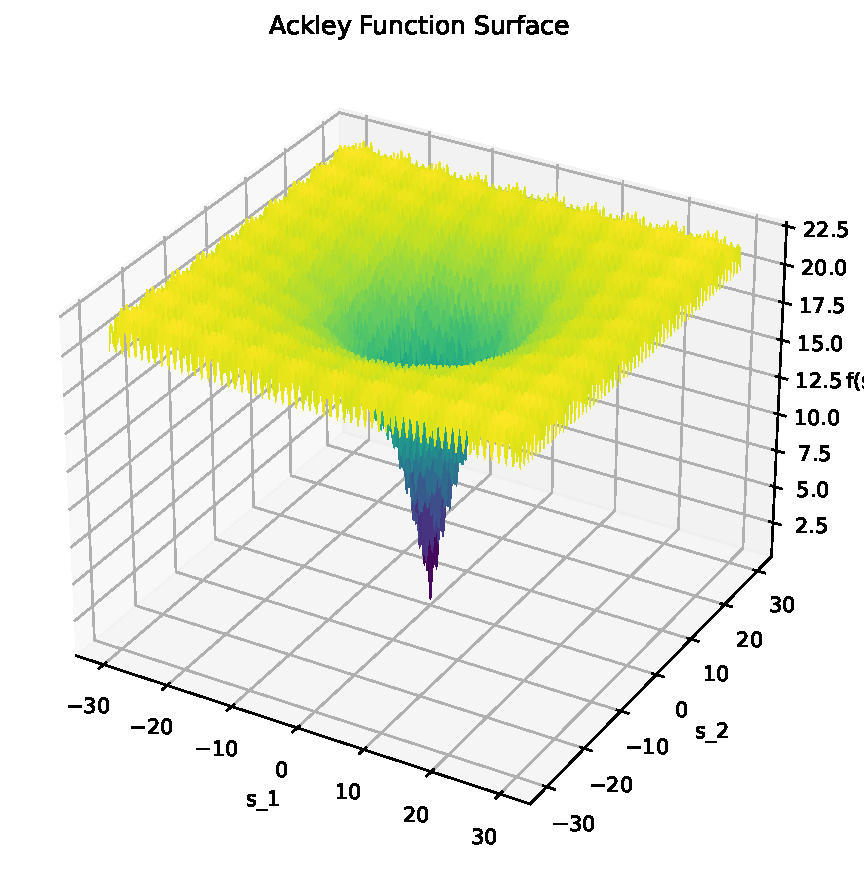
\includegraphics[keepaspectratio]{benchmark_files/figure-pdf/cell-4-output-2.pdf}}

\begin{itemize}
\tightlist
\item
  Example results: Vector s: {[}12.8 3.16{]}; Ackley function result:
  17.9
\item
  Distance from the Origin: The Ackley function reaches its global
  minimum of 0 at the origin (i.e., when both \(x_1\) and \(x_2\) are
  close to 0). Our vector values are quite far from the origin, which is
  why the function result is positive and relatively large at 17.9''
\item
  The Ackley landscape has an exponentially increasing structure as you
  move away from the global minimum. It has many local minima, which
  makes optimization algorithms prone to getting stuck in suboptimal
  solutions. A result like 17.9 is far from zero, and indicates that the
  vector is located in such a suboptimal region of the function space.
\item
  Thus, the Ackley result of 17.9 suggests that the point {[}12.8
  3.16{]}; is not close to the global minimum (which is zero at the
  origin) and is located in a region of higher function values.
\end{itemize}

\subsubsection{Differential Evolution with the Ackley
Function}\label{differential-evolution-with-the-ackley-function}

\begin{itemize}
\tightlist
\item
  To demonstrate how an algorithm does well on the Ackley function, we
  can use a global optimization algorithm such as Differential Evolution
  (DE), which is effective for non-convex functions with many local
  minima.
\item
  Differential Evolution (DE) is a population-based optimization
  algorithm used for solving complex multidimensional problems. It
  belongs to the family of evolutionary algorithms, where a population
  of candidate solutions evolves over time to find the global optimum of
  a function.
\item
  The differential\_evolution function from the scipy.optimize module is
  a powerful optimization tool designed to solve global optimization
  problems. It is a type of evolutionary algorithm, which is used when
  the function to optimize is non-linear, has many local minima, or is
  not differentiable.
\end{itemize}

\begin{Shaded}
\begin{Highlighting}[]
\ImportTok{import}\NormalTok{ numpy }\ImportTok{as}\NormalTok{ np}
\ImportTok{from}\NormalTok{ scipy.optimize }\ImportTok{import}\NormalTok{ differential\_evolution}
\ImportTok{import}\NormalTok{ matplotlib.pyplot }\ImportTok{as}\NormalTok{ plt}

\NormalTok{np.random.seed(}\DecValTok{5042}\NormalTok{)}

\CommentTok{\# Define the Ackley function}
\CommentTok{\# Ackley function implementation}
\KeywordTok{def}\NormalTok{ ackley(s):}
\NormalTok{    a, b, c }\OperatorTok{=} \DecValTok{20}\NormalTok{, }\FloatTok{0.2}\NormalTok{, }\DecValTok{2} \OperatorTok{*}\NormalTok{ np.pi}
\NormalTok{    n }\OperatorTok{=} \BuiltInTok{len}\NormalTok{(s)}
\NormalTok{    sum\_sq\_term }\OperatorTok{=}\NormalTok{ np.}\BuiltInTok{sum}\NormalTok{(s}\OperatorTok{**}\DecValTok{2}\NormalTok{)}
\NormalTok{    cos\_term }\OperatorTok{=}\NormalTok{ np.}\BuiltInTok{sum}\NormalTok{(np.cos(c }\OperatorTok{*}\NormalTok{ s))}
\NormalTok{    term1 }\OperatorTok{=} \OperatorTok{{-}}\NormalTok{a }\OperatorTok{*}\NormalTok{ np.exp(}\OperatorTok{{-}}\NormalTok{b }\OperatorTok{*}\NormalTok{ np.sqrt(sum\_sq\_term }\OperatorTok{/}\NormalTok{ n))}
\NormalTok{    term2 }\OperatorTok{=} \OperatorTok{{-}}\NormalTok{np.exp(cos\_term }\OperatorTok{/}\NormalTok{ n)}
    \ControlFlowTok{return}\NormalTok{ term1 }\OperatorTok{+}\NormalTok{ term2 }\OperatorTok{+}\NormalTok{ a }\OperatorTok{+}\NormalTok{ np.e}

\CommentTok{\# Set the bounds for the variables }
\NormalTok{bounds }\OperatorTok{=}\NormalTok{ [(}\OperatorTok{{-}}\DecValTok{30}\NormalTok{, }\DecValTok{30}\NormalTok{), (}\OperatorTok{{-}}\DecValTok{30}\NormalTok{, }\DecValTok{30}\NormalTok{)]}

\CommentTok{\# Use differential evolution to minimize the Ackley function}
\NormalTok{result }\OperatorTok{=}\NormalTok{ differential\_evolution(ackley, bounds, seed}\OperatorTok{=}\DecValTok{42}\NormalTok{)}

\CommentTok{\# Print the result}
\BuiltInTok{print}\NormalTok{(}\SpecialStringTok{f\textquotesingle{}Optimized parameters (x1, x2): }\SpecialCharTok{\{}\NormalTok{result}\SpecialCharTok{.}\NormalTok{x}\SpecialCharTok{\}}\SpecialStringTok{\textquotesingle{}}\NormalTok{)}
\BuiltInTok{print}\NormalTok{(}\SpecialStringTok{f\textquotesingle{}Function value at minimum: }\SpecialCharTok{\{}\NormalTok{result}\SpecialCharTok{.}\NormalTok{fun}\SpecialCharTok{\}}\SpecialStringTok{\textquotesingle{}}\NormalTok{)}


\CommentTok{\# Visualization of the Ackley function}
\NormalTok{x }\OperatorTok{=}\NormalTok{ np.linspace(}\OperatorTok{{-}}\DecValTok{30}\NormalTok{, }\DecValTok{30}\NormalTok{, }\DecValTok{400}\NormalTok{)}
\NormalTok{y }\OperatorTok{=}\NormalTok{ np.linspace(}\OperatorTok{{-}}\DecValTok{30}\NormalTok{, }\DecValTok{30}\NormalTok{, }\DecValTok{400}\NormalTok{)}
\NormalTok{X, Y }\OperatorTok{=}\NormalTok{ np.meshgrid(x, y)}

\CommentTok{\# Compute Z for the Ackley function}
\NormalTok{Z }\OperatorTok{=}\NormalTok{ np.array([ackley(np.array([x\_val, y\_val])) }\ControlFlowTok{for}\NormalTok{ x\_val, y\_val }\KeywordTok{in} \BuiltInTok{zip}\NormalTok{(np.ravel(X), np.ravel(Y))])}
\NormalTok{Z }\OperatorTok{=}\NormalTok{ Z.reshape(X.shape)}

\CommentTok{\# Plotting the Ackley function surface}
\NormalTok{fig }\OperatorTok{=}\NormalTok{ plt.figure(figsize}\OperatorTok{=}\NormalTok{(}\DecValTok{10}\NormalTok{, }\DecValTok{7}\NormalTok{))}
\NormalTok{ax }\OperatorTok{=}\NormalTok{ fig.add\_subplot(}\DecValTok{111}\NormalTok{, projection}\OperatorTok{=}\StringTok{\textquotesingle{}3d\textquotesingle{}}\NormalTok{)}
\NormalTok{ax.plot\_surface(X, Y, Z, cmap}\OperatorTok{=}\StringTok{\textquotesingle{}viridis\textquotesingle{}}\NormalTok{, edgecolor}\OperatorTok{=}\StringTok{\textquotesingle{}none\textquotesingle{}}\NormalTok{)}

\CommentTok{\# Customize the plot}
\NormalTok{ax.set\_title(}\StringTok{"Ackley Function Surface (2D)"}\NormalTok{)}
\NormalTok{ax.set\_xlabel(}\StringTok{"s\_1"}\NormalTok{)}
\NormalTok{ax.set\_ylabel(}\StringTok{"s\_2"}\NormalTok{)}
\NormalTok{ax.set\_zlabel(}\StringTok{"f(s)"}\NormalTok{)}

\CommentTok{\# Show the plot}
\NormalTok{plt.show()}
\end{Highlighting}
\end{Shaded}

\begin{verbatim}
Optimized parameters (x1, x2): [0. 0.]
Function value at minimum: 4.440892098500626e-16
\end{verbatim}

\pandocbounded{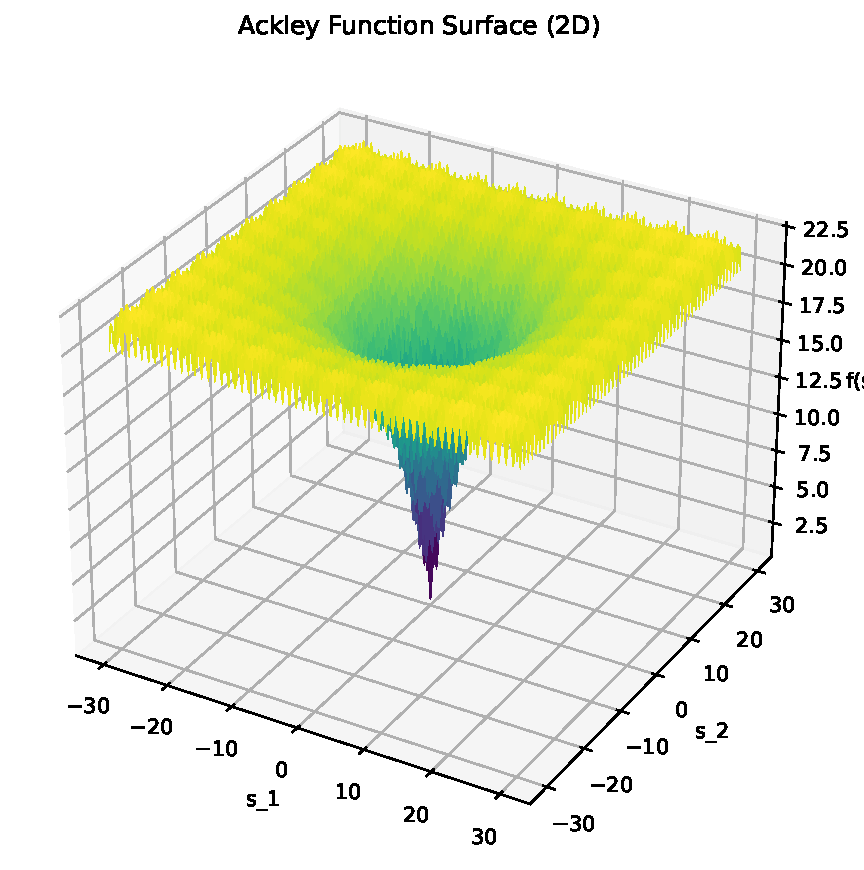
\includegraphics[keepaspectratio]{benchmark_files/figure-pdf/cell-5-output-2.pdf}}

\begin{itemize}
\tightlist
\item
  Using a great function that is designed to solve problems with
  multiple local minimums, you can see that we got extremely close to
  the local minimum 0.
\end{itemize}

\section{Multi-objective Optimization Problem
(MOP)}\label{multi-objective-optimization-problem-mop}

\begin{itemize}
\tightlist
\item
  Given a set of functions and a set of constraints, the MOP is to find
  the optimal value or a set of optimal values (also called Pareto
  front), subject to the constraints, out of all possible solutions of
  these functions.
\end{itemize}

\[\text{opt}\left( f_1(s), f_2(s), \dots, f_k(s) \right),
\quad \mathbf{s} \in \mathbb{R}^n, 
\quad \text{subject to } c_i(s) \odot b_i, \quad i = 1, 2, \dots, m,\]

\begin{itemize}
\tightlist
\item
  Where

  \begin{itemize}
  \tightlist
  \item
    \({R}^n\) and \({R}\) are the domain and codomain, respectively,
  \item
    \(f(s) {R}^n\) and \({R}\) is the objective function to be
    optimized,
  \item
    \(c_i(s): {R}^n\) and \({R}\odot b_i, \quad i = 1, 2, \ldots, m,\)
    are the constraints,
  \item
    and \(opt\) and \(\odot\) are as given in Definition 1 as \textless,
    \textgreater, =, ⩽, or ⩾.
  \end{itemize}
\end{itemize}

\subsection{The Schaffer min-min Multi-objective Optimization
Problem}\label{the-schaffer-min-min-multi-objective-optimization-problem}

\begin{itemize}
\tightlist
\item
  The Schaffer min-min problem is a well-known test function in the
  field of multi-objective optimization.
\item
  It is often used to evaluate optimization algorithms due to its
  simplicity and well-defined structure. The problem is particularly
  famous for having a simple Pareto-optimal front.
\item
  The Schaffer function can be defined as a two-objective optimization
  problem, where the objectives are functions of a single variable x.
\item
  The goal is to minimize both of these objective functions
  simultaneously.
\end{itemize}

\subsubsection{Characteristics and
Visualization}\label{characteristics-and-visualization}

\begin{itemize}
\tightlist
\item
  Convexity: The Pareto front of the Schaffer min-min problem is convex,
  making it relatively easy to identify the trade-off surface between
  the two objectives.
\item
  Uniqueness: The problem has a unique global Pareto-optimal front.
\item
  Complexity: Despite its simplicity, the problem is useful for
  benchmarking optimization algorithms, especially in multi-objective
  optimization.
\item
  Graphically, the Pareto front of the Schaffer min-min problem can be
  visualized as a curve in the objective space, where \(f_1(x)\) is
  plotted against \(f_2(x)\) and the curve represents the set of optimal
  trade-offs between the two objectives.
\end{itemize}

\pandocbounded{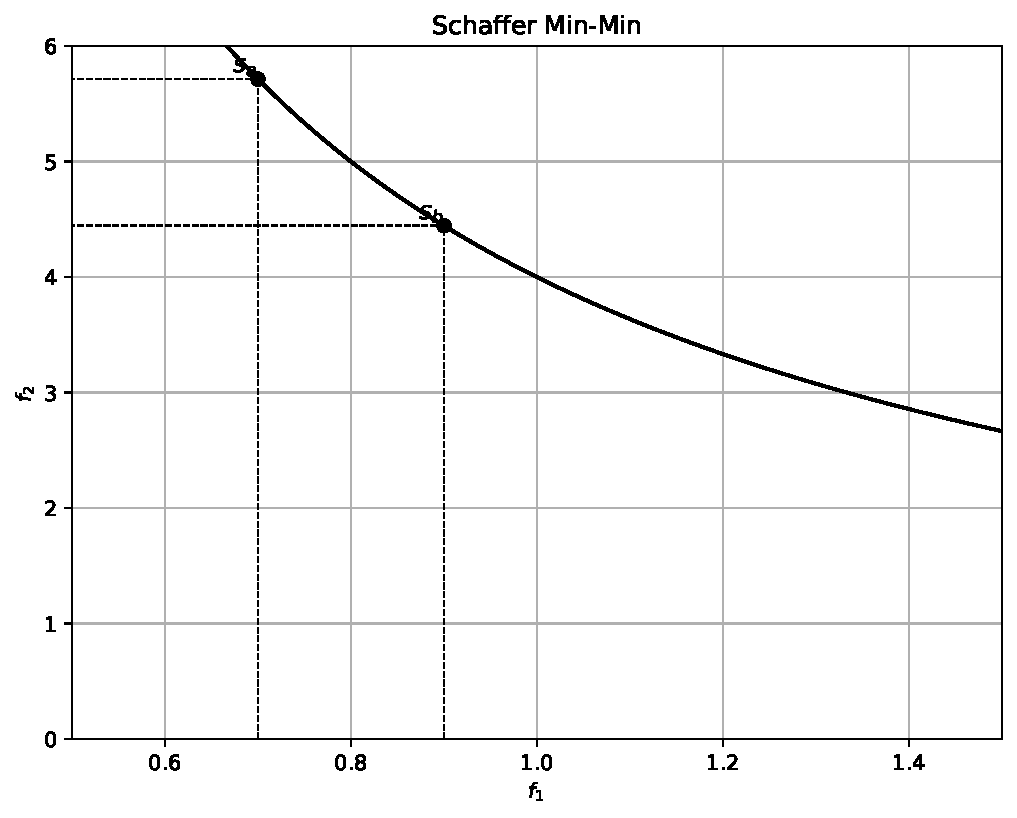
\includegraphics[keepaspectratio]{benchmark_files/figure-pdf/cell-6-output-1.pdf}}

\subsubsection{scipy.optimize import
minimize}\label{scipy.optimize-import-minimize}

\begin{itemize}
\tightlist
\item
  minimize is a general-purpose function from scipy.optimize used for
  finding the minimum of a scalar function.
\item
  Uses the BFGS (Broyden--Fletcher--Goldfarb--Shanno) algorithm when no
  specific method is provided. This method is a quasi-Newton
  optimization algorithm, particularly useful for smooth unconstrained
  problems.

  \begin{itemize}
  \tightlist
  \item
    It can handle different types of optimization problems, including:
    Unconstrained minimization
  \item
    Constrained minimization (equality and inequality constraints)
    Bounded minimization (where variables are limited to a certain
    range)
  \end{itemize}
\item
  Basic Workflow:

  \begin{itemize}
  \tightlist
  \item
    Define the objective function (the function to minimize). Choose an
    initial guess for the variables.
  \item
    Run the minimize function with the desired method.
  \item
    Analyze the results: returns optimized variables, the function
    value, and other diagnostic information.
  \end{itemize}
\end{itemize}

\subsubsection{Schaffer Min-Min Formula}\label{schaffer-min-min-formula}

\[
\min_{s \in \mathbb{R}^n} 
\begin{cases}
f_1(s) = s^2, \\
f_2(s) = (s - 2)^2,
\end{cases}
\quad \text{subject to} \quad s \in [-10^3, 10^3].
\]

\subsubsection{Schaffer Min-Min
Pseudocode}\label{schaffer-min-min-pseudocode}

\begin{Shaded}
\begin{Highlighting}[]
\NormalTok{Pseudocode}

\NormalTok{\# FUNCTION to calculate f1(s)}
\NormalTok{FUNCTION f1(s):}
\NormalTok{    RETURN s\^{}2}

\NormalTok{\# FUNCTION to calculate f2(s)}
\NormalTok{FUNCTION f2(s):}
\NormalTok{    RETURN (s {-} 2)\^{}2}

\NormalTok{\# FUNCTION for combined objective, weighted sum of f1 and f2}
\NormalTok{FUNCTION combined\_objective(s, w1=0.5, w2=0.5):}
\NormalTok{    RETURN w1 * f1(s) + w2 * f2(s)}

\NormalTok{\# MAIN EXECUTION}
\NormalTok{\# Step 1: Set up the bounds for the solution (s ∈ [{-}1000, 1000])}
\NormalTok{SET bounds = [{-}1000, 1000]}

\NormalTok{\# Step 2: Initialize a starting guess for the solution}
\NormalTok{SET initial\_guess = 0}

\NormalTok{\# Step 3: Minimize the combined objective function using an optimization algorithm}
\NormalTok{CALL minimize function with combined\_objective, initial\_guess, and bounds}
\NormalTok{STORE the result in result}

\NormalTok{\# Step 4: Print the optimization result}
\NormalTok{PRINT "Optimal value of s:", result.x}
\NormalTok{PRINT "f1(s):", f1(result.x)}
\NormalTok{PRINT "f2(s):", f2(result.x)}
\NormalTok{PRINT "Combined objective:", combined\_objective(result.x)}

\NormalTok{\# Step 5: Visualization {-} Create a range of values for s from {-}1000 to 1000}
\end{Highlighting}
\end{Shaded}

\subsubsection{Schaffer Min-Min Python
Implementation}\label{schaffer-min-min-python-implementation}

\begin{itemize}
\tightlist
\item
  Population Initialization: A population of random solutions is
  initialized within the bounds {[}−1000,1000{]}. Objective Function
  Evaluation: For each solution, both objective functions are evaluated.
\item
  Score Combination: The results of the two functions are combined into
  a single score, which can be minimized. In this case, the combination
  is a simple sum of f1 and f2.
\item
  Optimization Loop: Iteratively updates the solutions to find the
  minimum combined score using an optimization technique (e.g., gradient
  descent, genetic algorithm).
\end{itemize}

\begin{Shaded}
\begin{Highlighting}[]
\ImportTok{import}\NormalTok{ numpy }\ImportTok{as}\NormalTok{ np}
\ImportTok{from}\NormalTok{ scipy.optimize }\ImportTok{import}\NormalTok{ minimize}
\ImportTok{import}\NormalTok{ matplotlib.pyplot }\ImportTok{as}\NormalTok{ plt}


\CommentTok{\# Define the two objective functions for the Schaffer problem}
\KeywordTok{def}\NormalTok{ f1(s):}
    \ControlFlowTok{return}\NormalTok{ s}\OperatorTok{**}\DecValTok{2}

\KeywordTok{def}\NormalTok{ f2(s):}
    \ControlFlowTok{return}\NormalTok{ (s }\OperatorTok{{-}} \DecValTok{2}\NormalTok{)}\OperatorTok{**}\DecValTok{2}

\CommentTok{\# Combined objective function: weighted sum of f1 and f2}
\CommentTok{\# You can adjust the weights to explore different trade{-}offs between the two objectives}
\KeywordTok{def}\NormalTok{ combined\_objective(s, w1}\OperatorTok{=}\FloatTok{0.5}\NormalTok{, w2}\OperatorTok{=}\FloatTok{0.5}\NormalTok{):}
    \ControlFlowTok{return}\NormalTok{ w1 }\OperatorTok{*}\NormalTok{ f1(s) }\OperatorTok{+}\NormalTok{ w2 }\OperatorTok{*}\NormalTok{ f2(s)}

\CommentTok{\# Bounds for the solution (s ∈ [{-}1000, 1000])}
\NormalTok{bounds }\OperatorTok{=}\NormalTok{ [(}\OperatorTok{{-}}\DecValTok{1000}\NormalTok{, }\DecValTok{1000}\NormalTok{)]}

\CommentTok{\# Initial guess for the solution}
\NormalTok{initial\_guess }\OperatorTok{=}\NormalTok{ np.array([}\DecValTok{0}\NormalTok{])}

\CommentTok{\# Use scipy\textquotesingle{}s minimize function to find the solution}
\NormalTok{result }\OperatorTok{=}\NormalTok{ minimize(combined\_objective, initial\_guess, bounds}\OperatorTok{=}\NormalTok{bounds)}

\CommentTok{\# Print the result}
\BuiltInTok{print}\NormalTok{(}\StringTok{"Optimal value of s:"}\NormalTok{, result.x[}\DecValTok{0}\NormalTok{])}
\BuiltInTok{print}\NormalTok{(}\StringTok{"f1(s):"}\NormalTok{, f1(result.x[}\DecValTok{0}\NormalTok{]))}
\BuiltInTok{print}\NormalTok{(}\StringTok{"f2(s):"}\NormalTok{, f2(result.x[}\DecValTok{0}\NormalTok{]))}
\BuiltInTok{print}\NormalTok{(}\StringTok{"Combined objective:"}\NormalTok{, combined\_objective(result.x[}\DecValTok{0}\NormalTok{]))}

\CommentTok{\# Visualization of the objective functions and combined objective}
\NormalTok{s\_values }\OperatorTok{=}\NormalTok{ np.linspace(}\OperatorTok{{-}}\DecValTok{1000}\NormalTok{, }\DecValTok{1000}\NormalTok{, }\DecValTok{400}\NormalTok{)}
\NormalTok{f1\_values }\OperatorTok{=}\NormalTok{ f1(s\_values)}
\NormalTok{f2\_values }\OperatorTok{=}\NormalTok{ f2(s\_values)}
\NormalTok{combined\_values }\OperatorTok{=}\NormalTok{ combined\_objective(s\_values)}

\CommentTok{\# Plotting}
\NormalTok{plt.figure(figsize}\OperatorTok{=}\NormalTok{(}\DecValTok{10}\NormalTok{, }\DecValTok{6}\NormalTok{))}

\CommentTok{\# Plot f1(s), f2(s), and combined objective}
\NormalTok{plt.plot(s\_values, f1\_values, label}\OperatorTok{=}\StringTok{"f1(s) = s\^{}2"}\NormalTok{, color}\OperatorTok{=}\StringTok{\textquotesingle{}blue\textquotesingle{}}\NormalTok{)}
\NormalTok{plt.plot(s\_values, f2\_values, label}\OperatorTok{=}\StringTok{"f2(s) = (s {-} 2)\^{}2"}\NormalTok{, color}\OperatorTok{=}\StringTok{\textquotesingle{}green\textquotesingle{}}\NormalTok{)}
\NormalTok{plt.plot(s\_values, combined\_values, label}\OperatorTok{=}\StringTok{"Combined Objective"}\NormalTok{, color}\OperatorTok{=}\StringTok{\textquotesingle{}red\textquotesingle{}}\NormalTok{, linestyle}\OperatorTok{=}\StringTok{\textquotesingle{}{-}{-}\textquotesingle{}}\NormalTok{)}

\CommentTok{\# Mark the optimal solution found}
\NormalTok{plt.axvline(x}\OperatorTok{=}\NormalTok{result.x[}\DecValTok{0}\NormalTok{], color}\OperatorTok{=}\StringTok{\textquotesingle{}black\textquotesingle{}}\NormalTok{, linestyle}\OperatorTok{=}\StringTok{\textquotesingle{}:\textquotesingle{}}\NormalTok{, label}\OperatorTok{=}\SpecialStringTok{f"Optimal s = }\SpecialCharTok{\{}\NormalTok{result}\SpecialCharTok{.}\NormalTok{x[}\DecValTok{0}\NormalTok{]}\SpecialCharTok{:.2f\}}\SpecialStringTok{"}\NormalTok{)}

\CommentTok{\# Customize the plot}
\NormalTok{plt.title(}\StringTok{"Schaffer Min{-}Min Problem Visualization"}\NormalTok{)}
\NormalTok{plt.xlabel(}\StringTok{"s"}\NormalTok{)}
\NormalTok{plt.ylabel(}\StringTok{"Objective Function Value"}\NormalTok{)}
\NormalTok{plt.legend()}
\NormalTok{plt.grid(}\VariableTok{True}\NormalTok{)}

\CommentTok{\# Show the plot}
\NormalTok{plt.show()}
\end{Highlighting}
\end{Shaded}

\begin{verbatim}
Optimal value of s: 1.0000000134831095
f1(s): 1.0000000269662193
f2(s): 0.9999999730337812
Combined objective: 1.0000000000000002
\end{verbatim}

\pandocbounded{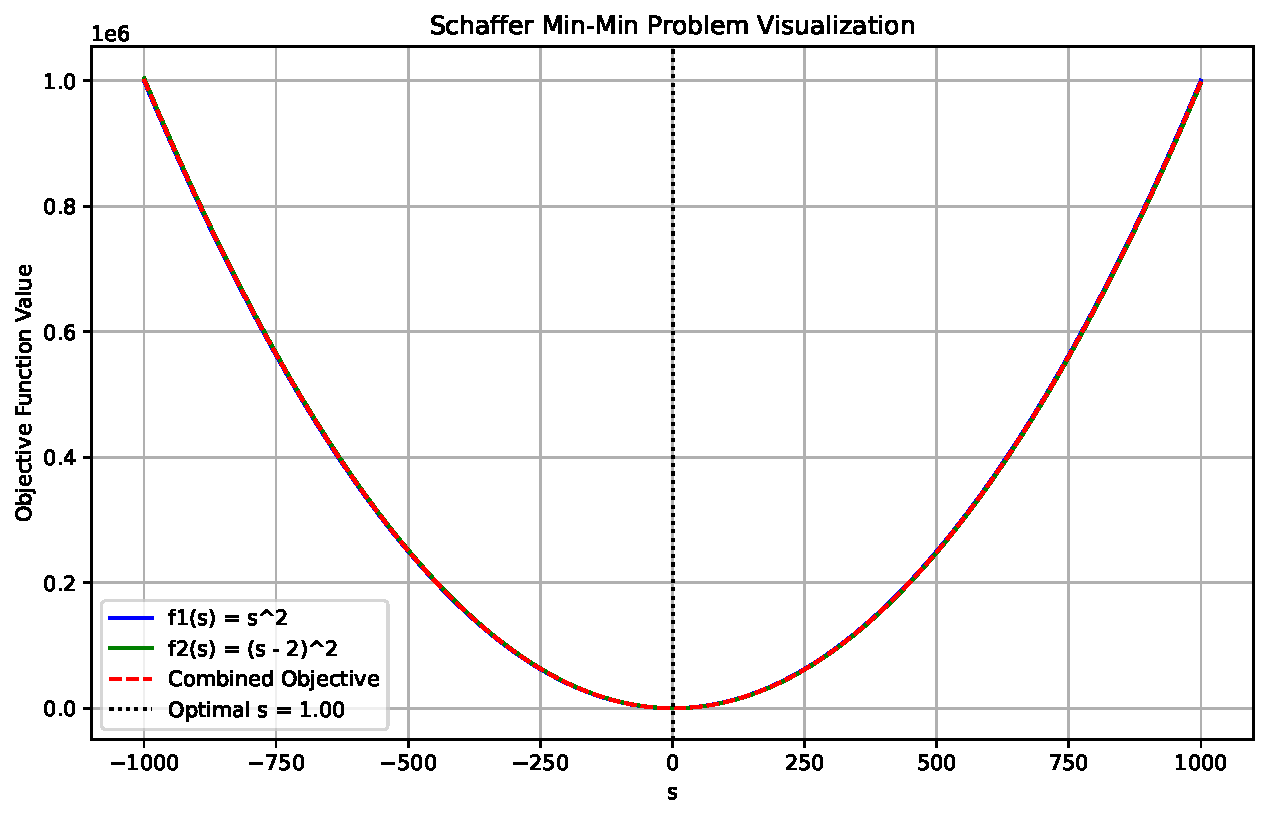
\includegraphics[keepaspectratio]{benchmark_files/figure-pdf/cell-7-output-2.pdf}}

\begin{itemize}
\tightlist
\item
  The results you achieved for the Schaffer Min-Min problem look
  excellent, as they closely approximate the optimal solution.
\item
  Optimal value of \(s\) we found is nearly exactly \(1\), the known
  optimal solution for the Schaffer function.

  \begin{itemize}
  \tightlist
  \item
    Objective function values: \(f_1(s) = s^2 = 1.000000027\)
  \item
    : \(f_2(s) = (s-2)^2 = 0.999999973\)
  \item
    These values are very close to 1 for both \(f_1\) and \(f_2\),
    indicating that the function values at this \(s\) are near-optimal.
  \end{itemize}
\item
  Combined objective: The combined objective (likely calculated as a
  weighted sum or some other combination of \(f_1\) and \(f_2\) is
  1.00000, which is extremely close to the expected combined optimal
  value of 1. This negligible difference suggests that the optimization
  algorithm has performed very well.
\end{itemize}

\bookmarksetup{startatroot}

\chapter{Using AI}\label{using-ai-3}

\begin{itemize}
\tightlist
\item
  Use the following prompt on a generative AI, like chatGPT, to learn
  more about the topics covered. ** evaluating optimization algorithms?
  Provide examples of their use in different domains.
\item
  Benchmark Problems Overview: What are benchmark problems, and why are
  they essential in evaluating optimization algorithms? Provide examples
  of their use in different domains.
\item
  Comparing Problems: Compare the OneMax problem, the Knapsack problem,
  and the Ackley function. Discuss the type of optimization each
  addresses and the challenges it presents.
\item
  Fitness Function: Write a Python function to evaluate the fitness of a
  binary string in the OneMax problem. Explain how this function helps
  in evolutionary algorithms.
\item
  Greedy vs Dynamic Programming: Solve the Fractional Knapsack problem
  using a greedy algorithm. Then, solve the 0/1 Knapsack problem using
  dynamic programming. Compare the results and explain the differences
  in their complexity and solutions.
\item
  Applications: Discuss real-world applications of the Knapsack problem.
  How do its constraints reflect practical optimization challenges?
\item
  Function Analysis: Explain why the Ackley function is challenging for
  optimization algorithms. What characteristics make it a good benchmark
  for multi-modal optimization?
\item
  Python Implementation: Use the provided Ackley function implementation
  to evaluate random points in the search space. Visualize the function
  in 3D and identify the global minimum.
\item
  Optimization Challenges: Discuss the concept of deception in B2D
  problems. Why is it critical for testing an algorithm's ability to
  escape local optima?
\item
  Schaffer Min-Min Problem: Solve the Schaffer Min-Min problem using a
  weighted sum approach. Experiment with different weight combinations
  and discuss how they affect the solution.
\end{itemize}

\bookmarksetup{startatroot}

\chapter{Conclusions}\label{conclusions-2}

\begin{itemize}
\item
  We introduced a set of popular optimization benchmark problems, widely
  used to evaluate the performance of various algorithms across
  different types of optimization challenges. These benchmarks include
  the OneMax Problem, which is commonly used in evolutionary algorithm
  research to assess an algorithm's capacity to evolve a binary string
  towards an optimal solution, specifically a string composed entirely
  of 1s. This problem is straightforward and serves as a foundation for
  evaluating basic evolutionary or heuristic methods. The Knapsack
  Problem is a classic combinatorial, NP-complete problem that tests
  algorithms' abilities to maximize the total value of selected items
  without exceeding a weight limit. This problem is pivotal in assessing
  algorithms designed for discrete optimization tasks, where finding an
  optimal solution is computationally intensive.
\item
  The Binary-to-Decimal (B2D) Problem introduces a deceptive landscape
  that misleads optimization algorithms toward suboptimal solutions. It
  is particularly useful for testing whether an algorithm can avoid
  getting trapped in local optima and demonstrates the importance of
  incorporating diversity strategies like mutation in evolutionary
  algorithms.
\item
  The Ackley Function represents a single continuous optimization
  benchmark with a highly multi-modal landscape. It is challenging due
  to its numerous local minima, making it ideal for testing an
  algorithm's ability to balance exploration and exploitation in
  continuous search spaces. In multi-objective optimization, the
  Schaffer Min-Min Problem serves as a benchmark, presenting a simple
  yet effective test for algorithms to identify Pareto-optimal
  solutions, as it requires the simultaneous minimization of two
  objectives. Collectively, these benchmark problems allow researchers
  and practitioners to compare the strengths and limitations of
  optimization algorithms across both discrete and continuous scenarios.
\end{itemize}

\bookmarksetup{startatroot}

\chapter{Exhaustive Search}\label{exhaustive-search}

\begin{itemize}
\item
  If you had unlimited time to search through every possible hobby in
  the world, which one do you think you'd end up pursuing?
\item
  Exhaustive Search (also known as brute-force search) is a
  problem-solving technique that systematically enumerates all possible
  solutions to find the best one.
\item
  It evaluates every potential solution against the objective function
  and selects the optimal one.
\item
  When to use: When the problem size is small and when optimality is
  critical and computation time is feasible.
\item
  Limitations: Computationally expensive. Not feasible for large problem
  spaces due to exponential time complexity.
\end{itemize}

\section{Advantages and Disadvantages of
ES}\label{advantages-and-disadvantages-of-es}

\begin{itemize}
\tightlist
\item
  Advantages:

  \begin{itemize}
  \tightlist
  \item
    Guaranteed Optimal Solution: Finds the best possible solution,
    ensuring optimality.
  \item
    Simplicity: Easy to understand and implement for small-scale
    problems.
  \end{itemize}
\item
  Disadvantages:

  \begin{itemize}
  \tightlist
  \item
    Scalability Issues: Infeasible for large datasets due to exponential
    time complexity.
  \item
    Resource Intensive: High computational cost in terms of time and
    memory.
  \end{itemize}
\end{itemize}

\subsection{Exhaustive Search
Algorithm}\label{exhaustive-search-algorithm}

\begin{itemize}
\tightlist
\item
  Check all the candidate solutions in the solution space of the problem
  in question; therefore, it is always capable of finding the best
  solution for the problem in question.
\end{itemize}

\begin{figure}[H]

{\centering \pandocbounded{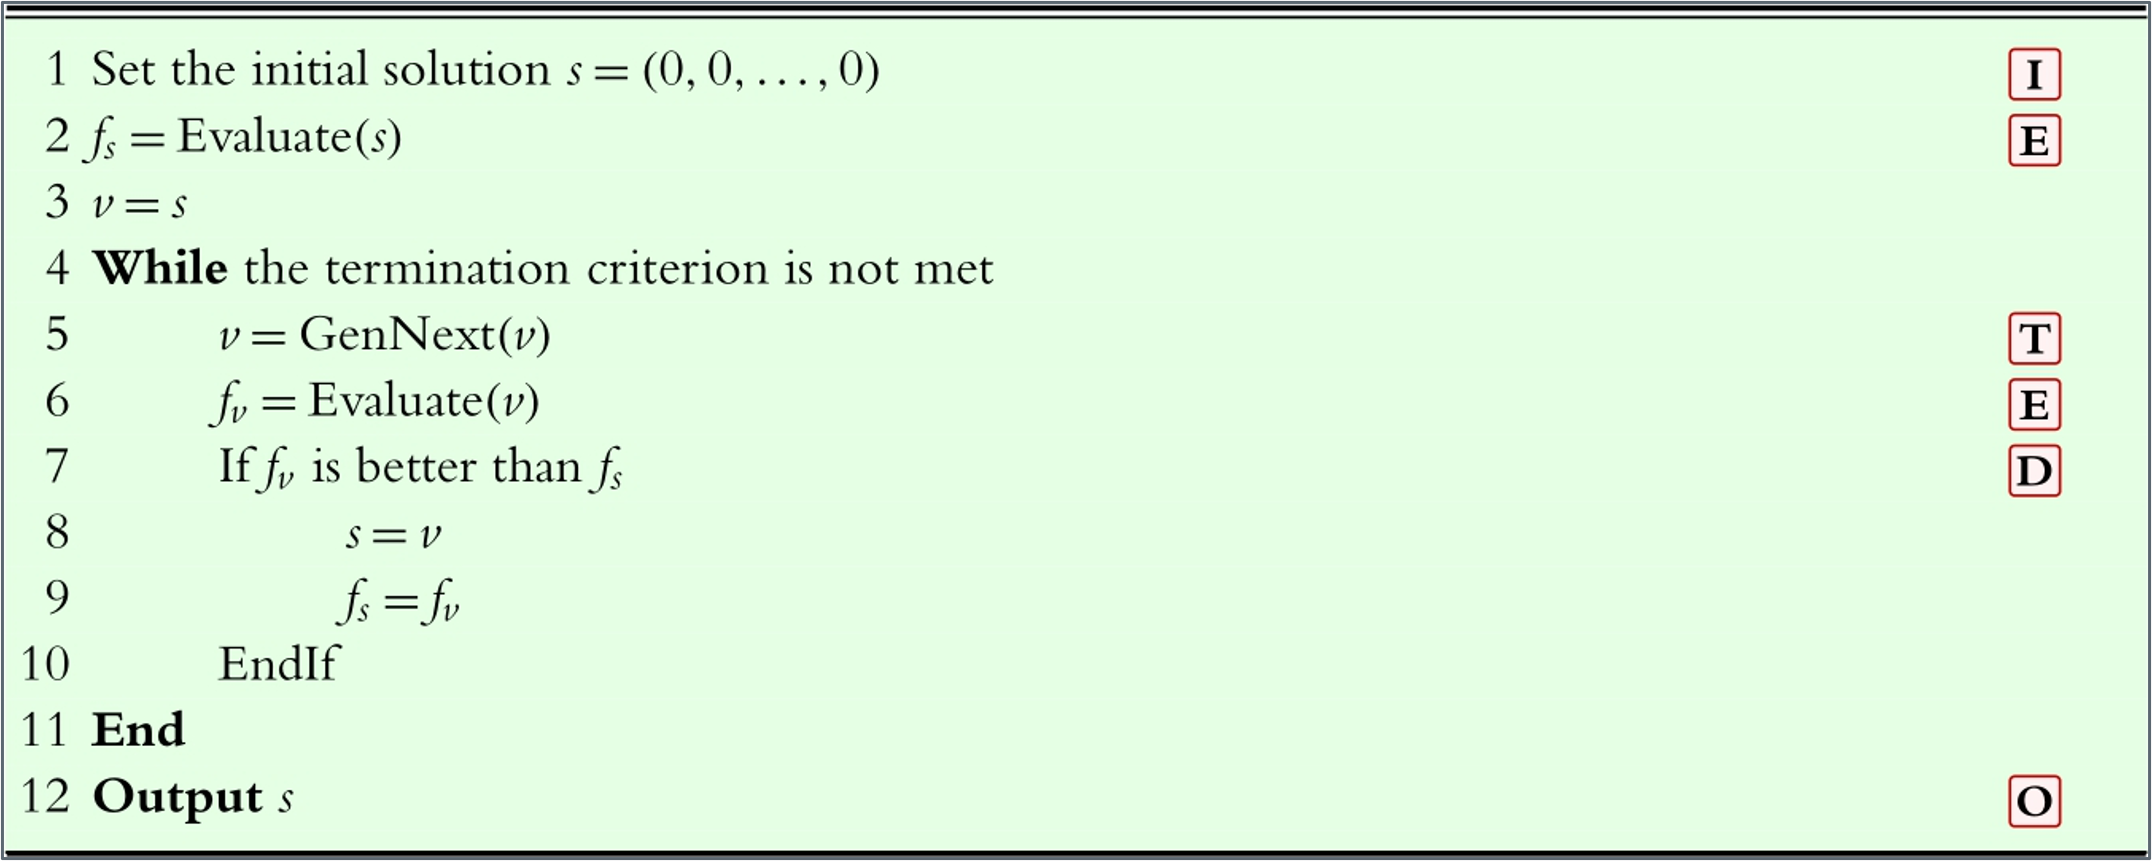
\includegraphics[keepaspectratio]{Pictures/es.png}}

}

\caption{es algorithm}

\end{figure}%

\section{Exhaustive Search in Continuous vs.~Discrete
Domains}\label{exhaustive-search-in-continuous-vs.-discrete-domains}

\begin{itemize}
\tightlist
\item
  Continuous Domains: Require discretization (using a step size) to make
  exhaustive search feasible.

  \begin{itemize}
  \tightlist
  \item
    Example: Ackley function.
  \end{itemize}
\item
  Discrete Domains: Solutions can be explicitly enumerated without
  discretization.

  \begin{itemize}
  \tightlist
  \item
    Example: Knapsack problem.
  \end{itemize}
\item
  Challenges in Continuous Domains:

  \begin{itemize}
  \tightlist
  \item
    Infinite solution space makes direct enumeration impossible.
  \item
    Step size is critical for balancing resolution and computational
    cost.
  \end{itemize}
\end{itemize}

\subsection{Role of Step Size in Continuous
Optimization}\label{role-of-step-size-in-continuous-optimization}

\begin{itemize}
\tightlist
\item
  Why Step Size Matters: Controls the granularity of the search.

  \begin{itemize}
  \tightlist
  \item
    Smaller steps increase resolution but significantly raise
    computation time.
  \item
    Larger steps reduce computational cost but risk missing the optimal
    solution.
  \end{itemize}
\item
  Practical Considerations:

  \begin{itemize}
  \tightlist
  \item
    Optimal step size depends on the problem's scale and the required
    precision.
  \item
    Trade-off between efficiency and accuracy.
  \end{itemize}
\item
  When is Exhaustive Search Practical?

  \begin{itemize}
  \tightlist
  \item
    Discrete Domains:

    \begin{itemize}
    \tightlist
    \item
      Feasible if the solution space is small (manageable number of
      combinations).
    \item
      Guarantees finding the exact optimal solution.
    \end{itemize}
  \item
    Continuous Domains:

    \begin{itemize}
    \tightlist
    \item
      Only practical when the domain is small and can be discretized
      effectively.
    \end{itemize}
  \item
    Higher dimensions increase complexity exponentially (curse of
    dimensionality).
  \end{itemize}
\end{itemize}

\section{The Search Strategy of ES}\label{the-search-strategy-of-es}

\pandocbounded{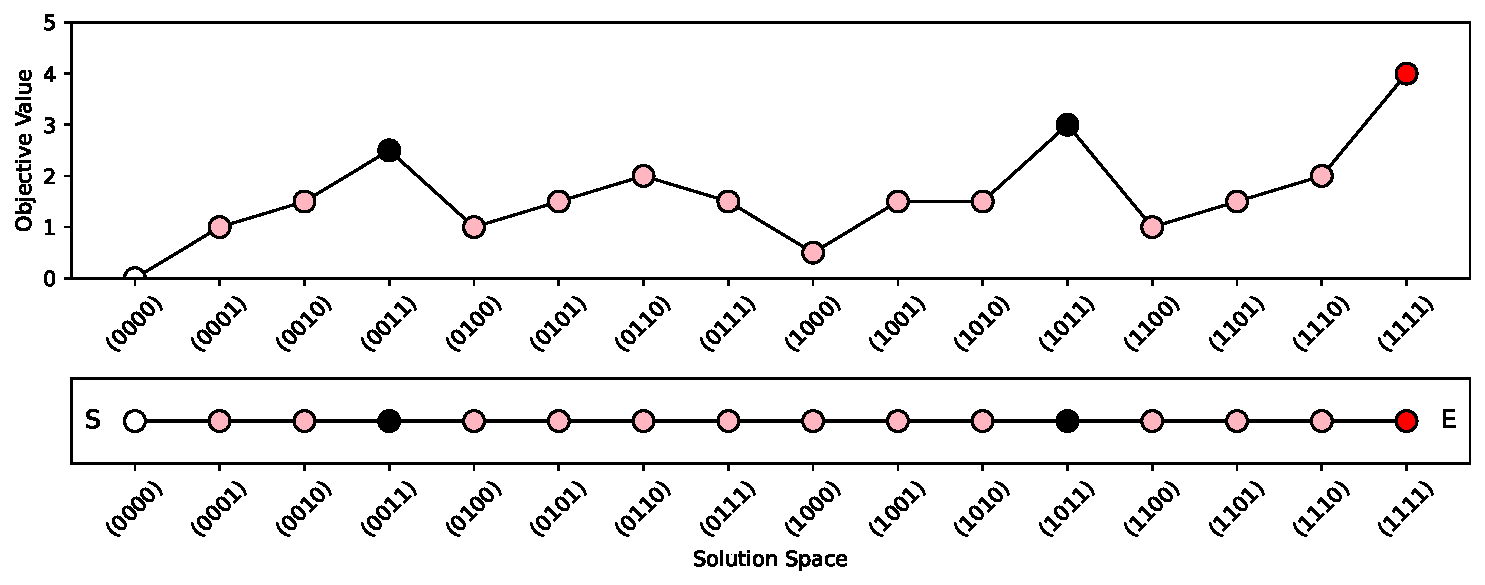
\includegraphics[keepaspectratio]{es_files/figure-pdf/cell-2-output-1.pdf}}

\bookmarksetup{startatroot}

\chapter{Knapsack Problem Example of
ES}\label{knapsack-problem-example-of-es}

\begin{itemize}
\tightlist
\item
  Finding Optimal Subset of Items to Max Value in Knapsack Problem using
  Exhaustive Search
\end{itemize}

\begin{Shaded}
\begin{Highlighting}[]
\ImportTok{from}\NormalTok{ itertools }\ImportTok{import}\NormalTok{ combinations}

\CommentTok{\# Define the items and maximum weight}
\NormalTok{items }\OperatorTok{=}\NormalTok{ [}
\NormalTok{    \{}\StringTok{"weight"}\NormalTok{: }\DecValTok{3}\NormalTok{, }\StringTok{"value"}\NormalTok{: }\DecValTok{4}\NormalTok{\},  }\CommentTok{\# Item 1}
\NormalTok{    \{}\StringTok{"weight"}\NormalTok{: }\DecValTok{4}\NormalTok{, }\StringTok{"value"}\NormalTok{: }\DecValTok{5}\NormalTok{\},  }\CommentTok{\# Item 2}
\NormalTok{    \{}\StringTok{"weight"}\NormalTok{: }\DecValTok{7}\NormalTok{, }\StringTok{"value"}\NormalTok{: }\DecValTok{10}\NormalTok{\}  }\CommentTok{\# Item 3}
\NormalTok{]}
\NormalTok{max\_weight }\OperatorTok{=} \DecValTok{10}

\CommentTok{\# Exhaustive search function with while loop to solve the knapsack problem}
\KeywordTok{def}\NormalTok{ knapsack\_exhaustive\_while(items, max\_weight):}
\NormalTok{    best\_value }\OperatorTok{=} \DecValTok{0}
\NormalTok{    best\_combination }\OperatorTok{=}\NormalTok{ []}

\NormalTok{    r }\OperatorTok{=} \DecValTok{1}
    \ControlFlowTok{while}\NormalTok{ r }\OperatorTok{\textless{}=} \BuiltInTok{len}\NormalTok{(items):  }\CommentTok{\# Iterating over different combination sizes}
\NormalTok{        combos }\OperatorTok{=} \BuiltInTok{list}\NormalTok{(combinations(items, r))}
\NormalTok{        i }\OperatorTok{=} \DecValTok{0}
        \ControlFlowTok{while}\NormalTok{ i }\OperatorTok{\textless{}} \BuiltInTok{len}\NormalTok{(combos):  }\CommentTok{\# Iterating over each combination}
\NormalTok{            combo }\OperatorTok{=}\NormalTok{ combos[i]}
\NormalTok{            weight }\OperatorTok{=} \BuiltInTok{sum}\NormalTok{(item[}\StringTok{\textquotesingle{}weight\textquotesingle{}}\NormalTok{] }\ControlFlowTok{for}\NormalTok{ item }\KeywordTok{in}\NormalTok{ combo)}
\NormalTok{            value }\OperatorTok{=} \BuiltInTok{sum}\NormalTok{(item[}\StringTok{\textquotesingle{}value\textquotesingle{}}\NormalTok{] }\ControlFlowTok{for}\NormalTok{ item }\KeywordTok{in}\NormalTok{ combo)}

            \ControlFlowTok{if}\NormalTok{ weight }\OperatorTok{\textless{}=}\NormalTok{ max\_weight }\KeywordTok{and}\NormalTok{ value }\OperatorTok{\textgreater{}}\NormalTok{ best\_value:}
\NormalTok{                best\_value }\OperatorTok{=}\NormalTok{ value}
\NormalTok{                best\_combination }\OperatorTok{=}\NormalTok{ combo}

\NormalTok{            i }\OperatorTok{+=} \DecValTok{1}  \CommentTok{\# Moving to the next combination}
\NormalTok{        r }\OperatorTok{+=} \DecValTok{1}  \CommentTok{\# Increasing the size of combinations to check}

    \ControlFlowTok{return}\NormalTok{ best\_value, best\_combination}

\CommentTok{\# Run the exhaustive search knapsack algorithm}
\NormalTok{best\_value, best\_combination }\OperatorTok{=}\NormalTok{ knapsack\_exhaustive\_while(items, max\_weight)}

\KeywordTok{def}\NormalTok{ print\_results(best\_value, best\_combination):}
    \BuiltInTok{print}\NormalTok{(}\StringTok{"Optimal items selected:"}\NormalTok{)}
    \ControlFlowTok{for}\NormalTok{ item }\KeywordTok{in}\NormalTok{ best\_combination:}
        \BuiltInTok{print}\NormalTok{(}\SpecialStringTok{f"Item with weight: }\SpecialCharTok{\{}\NormalTok{item[}\StringTok{\textquotesingle{}weight\textquotesingle{}}\NormalTok{]}\SpecialCharTok{\}}\SpecialStringTok{ and value: }\SpecialCharTok{\{}\NormalTok{item[}\StringTok{\textquotesingle{}value\textquotesingle{}}\NormalTok{]}\SpecialCharTok{\}}\SpecialStringTok{"}\NormalTok{)}
    \BuiltInTok{print}\NormalTok{(}\SpecialStringTok{f"Total Value: }\SpecialCharTok{\{}\NormalTok{best\_value}\SpecialCharTok{\}}\SpecialStringTok{"}\NormalTok{)}
    
\CommentTok{\# Print the results}
\NormalTok{print\_results(best\_value, best\_combination)}
\end{Highlighting}
\end{Shaded}

\begin{verbatim}
Optimal items selected:
Item with weight: 3 and value: 4
Item with weight: 7 and value: 10
Total Value: 14
\end{verbatim}

\begin{itemize}
\tightlist
\item
  Step 1: Calculate Ratios

  \begin{itemize}
  \tightlist
  \item
    \(wv1 = 4/3 = 1.333\)
  \item
    \(wv2 = 5/4 = 1.25\)
  \item
    \(wv3 = 10/7 = 1.428571\)
  \end{itemize}
\item
  Step 2: Order by Ratio (High to Low)

  \begin{itemize}
  \tightlist
  \item
    \(wv3\) at \(1.43\)
  \item
    \(wv1\) at \(1.333\)
  \item
    \(wv2\) at \(1.25\)
  \end{itemize}
\item
  Step 3: Fill the Sack

  \begin{itemize}
  \tightlist
  \item
    Add \{7:10 and then 3:4\} filled to 10 weight
  \item
    Optimal items: (\{`weight': 3, `value': 4\}, \{`weight': 7, `value':
    10\}), Total Value: 14
  \end{itemize}
\end{itemize}

\bookmarksetup{startatroot}

\chapter{ES with a One Max Problem}\label{es-with-a-one-max-problem}

\section{Algorithmic Steps of ES}\label{algorithmic-steps-of-es}

\begin{itemize}
\item
  For each binary solution (up to num\_bits length), the code evaluates
  the number of 1's in its binary representation (which is used as the
  ``fitness'' value).
\item
  It then finds the solution with the highest number of 1's (the one
  with the most bits set to 1).
\item
  Import necessary tools: time for timing and matplotlib for plotting
  results.
\item
  Set up run function

  \begin{itemize}
  \tightlist
  \item
    Loop through all possible solutions.
  \item
    Evaluate each one and track its fitness.
  \item
    Update the best solution as needed.
  \item
    Return the best solution and fitness progress.
  \end{itemize}
\item
  Define helper functions:

  \begin{itemize}
  \tightlist
  \item
    Transit: Move to the next solution.
  \item
    Evaluate: Count the number of 1s in the binary version of the
    solution (higher is better).
  \item
    Determine: Compare fitness in order to track the best solution found
    so far.
  \end{itemize}
\end{itemize}

\section{Imports}\label{imports}

\begin{Shaded}
\begin{Highlighting}[]
\ImportTok{import}\NormalTok{ time}
\ImportTok{import}\NormalTok{ matplotlib.pyplot }\ImportTok{as}\NormalTok{ plt}
\end{Highlighting}
\end{Shaded}

\section{run\_exhaustive\_search
function}\label{run_exhaustive_search-function}

\begin{itemize}
\tightlist
\item
  run\_exhaustive\_search(num\_bits):
\item
  Calculates the total number of possible solutions max\_sol is the
  maximum possible solution, which is \(2^{numbits}\). \(2 ** numbits\):
  This correctly represents the total number of possible combinations
  when you have numbits binary bits. For example, if numbits = 3, the
  possible solutions range from \(000 (0)\) to \(111 (7)\), resulting in
  \(2^3=8\) solutions.
\item
  Initializes \(s\) is the current solution, initially set to 0.
\item
  Initializes \(best_fitness\) and \(best_solution\) to track the best
  results.
\item
  Initializes an empty list \(fitness_over_time\) to track the fitness
  at each step.
\end{itemize}

\begin{Shaded}
\begin{Highlighting}[]
\CommentTok{\# Function for initialization (I)}
\KeywordTok{def}\NormalTok{ init\_es(num\_bits}\OperatorTok{=}\DecValTok{10}\NormalTok{):}
\NormalTok{    max\_sol }\OperatorTok{=} \DecValTok{2} \OperatorTok{**}\NormalTok{ num\_bits  }\CommentTok{\# Total number of solutions}
\NormalTok{    s }\OperatorTok{=} \DecValTok{0}  \CommentTok{\# Step 1: Set the initial solution s = (0)}
\NormalTok{    f\_s }\OperatorTok{=}\NormalTok{ evaluate(s)  }\CommentTok{\# Step 2: Evaluate initial solution}
    \ControlFlowTok{return}\NormalTok{ s, f\_s, max\_sol}
\end{Highlighting}
\end{Shaded}

\section{Helper Functions}\label{helper-functions}

\begin{itemize}
\tightlist
\item
  transit(s): Simply increments the current solution by 1.
\end{itemize}

\begin{Shaded}
\begin{Highlighting}[]
\CommentTok{\# Function for transit (T)}
\KeywordTok{def}\NormalTok{ transit(s):}
\NormalTok{    s }\OperatorTok{+=} \DecValTok{1}
    \ControlFlowTok{return}\NormalTok{ s}
\end{Highlighting}
\end{Shaded}

\begin{itemize}
\tightlist
\item
  evaluate(s): Evaluates the ``fitness'' of the solution by counting how
  many 1's are present in its binary representation. The more 1's, the
  better the solution.
\end{itemize}

\begin{Shaded}
\begin{Highlighting}[]
\CommentTok{\# Function for evaluation (E)}
\KeywordTok{def}\NormalTok{ evaluate(s):}
    \ControlFlowTok{return} \BuiltInTok{bin}\NormalTok{(s).count(}\StringTok{"1"}\NormalTok{)  }\CommentTok{\# Counts the number of 1s in the binary representation of s}
\end{Highlighting}
\end{Shaded}

\begin{itemize}
\tightlist
\item
  determine(fv, v, fs, s): This method checks whether the fitness of the
  new solution (fv) is greater than the current best fitness (fs). If
  so, it updates the current best solution and fitness.
\end{itemize}

\begin{Shaded}
\begin{Highlighting}[]
\CommentTok{\# Function for determine (D)}
\KeywordTok{def}\NormalTok{ determine(fv, v, fs, s):}
    \ControlFlowTok{if}\NormalTok{ fv }\OperatorTok{\textgreater{}}\NormalTok{ fs:}
\NormalTok{        fs, s }\OperatorTok{=}\NormalTok{ fv, v}
    \ControlFlowTok{return}\NormalTok{ fs, s}
\end{Highlighting}
\end{Shaded}

\section{Main Loop}\label{main-loop}

\begin{itemize}
\tightlist
\item
  A while loop iterates through all possible solutions (represented by
  s). For each solution s, it calculates the fitness using the
  evaluate() function.

  \begin{itemize}
  \tightlist
  \item
    fitness is the ``fitness'' score of the current solution, calculated
    using evaluate(s) (which counts the number of 1's in the binary
    representation of s).
  \item
    The loop continues until all possible solutions (v from 0 to
    max\_sol) have been evaluated.
  \end{itemize}
\item
  Appends the fitness value to fitness\_over\_time.

  \begin{itemize}
  \tightlist
  \item
    determine() updates fs (fitness) and s (solution) if the new
    solution (v) has a higher fitness.
  \end{itemize}
\item
  If the current solution has a better fitness than the best found so
  far, it updates the best fitness and solution.

  \begin{itemize}
  \tightlist
  \item
    For each iteration, the solution is updated (transit method),
    evaluated (evaluate method), and the best solution is determined
    (determine method).
  \end{itemize}
\item
  Return Values: Returns fitness\_over\_time and best\_solution after
  completing the exhaustive search.
\end{itemize}

\begin{Shaded}
\begin{Highlighting}[]
\CommentTok{\# Run function for exhaustive search}
\KeywordTok{def}\NormalTok{ run\_exhaustive\_search(num\_bits}\OperatorTok{=}\DecValTok{10}\NormalTok{):}
    \CommentTok{\# Initialize using init\_es}
\NormalTok{    s, f\_s, max\_sol }\OperatorTok{=}\NormalTok{ init\_es(num\_bits)}
    
    \CommentTok{\#Set v = s}
\NormalTok{    best\_solution }\OperatorTok{=}\NormalTok{ s}
\NormalTok{    best\_fitness }\OperatorTok{=}\NormalTok{ f\_s}
    
\NormalTok{    fitness\_over\_time }\OperatorTok{=}\NormalTok{ []}
    
    \CommentTok{\# While the termination criterion is not met}
    \ControlFlowTok{while}\NormalTok{ s }\OperatorTok{\textless{}}\NormalTok{ max\_sol:}
        \CommentTok{\# Generate the next solution v = GenNext(v)}
\NormalTok{        v }\OperatorTok{=}\NormalTok{ s}
        
        \CommentTok{\# Evaluate the new solution}
\NormalTok{        f\_v }\OperatorTok{=}\NormalTok{ evaluate(v)}
        
        \CommentTok{\# Track fitness over time for plotting}
\NormalTok{        fitness\_over\_time.append(f\_v)}
        
        \CommentTok{\# Print current solution and its fitness: Print command commented out for simplicity because it prints all the comparisons. }
        \CommentTok{\#print(f"\{f\_v\} \# \{v:0\{num\_bits\}b\}")}
        
        \CommentTok{\#If f\_v is better than f\_s, update s = v, f\_s = f\_v}
        \ControlFlowTok{if}\NormalTok{ f\_v }\OperatorTok{\textgreater{}}\NormalTok{ f\_s:}
\NormalTok{            best\_solution }\OperatorTok{=}\NormalTok{ v}
\NormalTok{            best\_fitness }\OperatorTok{=}\NormalTok{ f\_v}
        
        \CommentTok{\#continued: Move to the next solution}
\NormalTok{        s }\OperatorTok{+=} \DecValTok{1}  \CommentTok{\# Increment solution}
    
    \CommentTok{\#Returned for Output the best solution}
    \ControlFlowTok{return}\NormalTok{ fitness\_over\_time, best\_solution}
\end{Highlighting}
\end{Shaded}

\section{Main Execution}\label{main-execution}

\begin{itemize}
\tightlist
\item
  In exhaustive search, the ``main execution'' often focuses on setting
  the number of bits because exhaustive search involves systematically
  evaluating all possible solutions in the search space. When the
  solutions are represented as binary strings, the number of bits
  directly determines the size of the search space.
\item
  Why it matters:

  \begin{itemize}
  \tightlist
  \item
    Defining the Search Space: The number of bits defines how many
    unique binary strings (or configurations) are possible. For \(2^n\)
    possible combinations. So, by setting the number of bits, you are
    effectively defining the boundaries of the search space.
  \item
    Enumerating All Possibilities: In exhaustive search, the algorithm
    needs to evaluate every possible configuration to ensure the optimal
    solution is found. Each unique binary string corresponds to a
    specific candidate solution, so having the number of bits set
    enables the algorithm to enumerate all possible configurations.
  \item
    Computational Complexity: The number of bits directly affects the
    computational complexity of exhaustive search. With \(n\) bits, the
    search space grows exponentially, which is manageable for small
    \(n\) but quickly becomes infeasible for larger \(n\). By
    controlling the number of bits, you also control the practical
    feasibility of the exhaustive search.
  \end{itemize}
\end{itemize}

Simplicity: Since exhaustive search doesn't involve complex heuristics
or probabilistic methods, setting the number of bits becomes the main
task. The rest of the algorithm is straightforward: generate each binary
string, evaluate its objective value, and keep track of the best
solution.

\begin{Shaded}
\begin{Highlighting}[]
\CommentTok{\# Main execution}
\NormalTok{num\_bits }\OperatorTok{=} \DecValTok{10}  \CommentTok{\# You can adjust the number of bits}
\end{Highlighting}
\end{Shaded}

\section{Output}\label{output}

\begin{Shaded}
\begin{Highlighting}[]
\CommentTok{\# Run the exhaustive search and get fitness values}
\NormalTok{start\_time }\OperatorTok{=}\NormalTok{ time.time()}
\NormalTok{fitness\_over\_time, best\_solution }\OperatorTok{=}\NormalTok{ run\_exhaustive\_search(num\_bits)}
\NormalTok{end\_time }\OperatorTok{=}\NormalTok{ time.time()}
\NormalTok{execution\_time }\OperatorTok{=}\NormalTok{ end\_time }\OperatorTok{{-}}\NormalTok{ start\_time  }\CommentTok{\# Calculate elapsed time}

\CommentTok{\# Output (O)}
\BuiltInTok{print}\NormalTok{(}\SpecialStringTok{f"Exhaustive Search One{-}Max Time elapsed: }\SpecialCharTok{\{}\NormalTok{execution\_time}\SpecialCharTok{:.6f\}}\SpecialStringTok{ seconds"}\NormalTok{)  }\CommentTok{\# Print the elapsed time}
\BuiltInTok{print}\NormalTok{(}\SpecialStringTok{f"\# name of the search algorithm: Exhaustive Search"}\NormalTok{)}
\BuiltInTok{print}\NormalTok{(}\SpecialStringTok{f"\# number of bits: }\SpecialCharTok{\{}\NormalTok{num\_bits}\SpecialCharTok{\}}\SpecialStringTok{"}\NormalTok{)}

\CommentTok{\# Plot the evolution of fitness over time}
\NormalTok{plt.figure(figsize}\OperatorTok{=}\NormalTok{(}\DecValTok{10}\NormalTok{, }\DecValTok{6}\NormalTok{))}
\NormalTok{plt.plot(fitness\_over\_time, label}\OperatorTok{=}\StringTok{\textquotesingle{}Fitness over time\textquotesingle{}}\NormalTok{, color}\OperatorTok{=}\StringTok{\textquotesingle{}blue\textquotesingle{}}\NormalTok{, linewidth}\OperatorTok{=}\DecValTok{2}\NormalTok{)}
\NormalTok{plt.title(}\SpecialStringTok{f\textquotesingle{}Exhaustive Search: Fitness Evolution (}\SpecialCharTok{\{}\NormalTok{num\_bits}\SpecialCharTok{\}}\SpecialStringTok{ bits)\textquotesingle{}}\NormalTok{)}
\NormalTok{plt.xlabel(}\StringTok{\textquotesingle{}Evaluations\textquotesingle{}}\NormalTok{)}
\NormalTok{plt.ylabel(}\StringTok{\textquotesingle{}Fitness (Number of 1s)\textquotesingle{}}\NormalTok{)}
\NormalTok{plt.grid(}\VariableTok{True}\NormalTok{)}
\NormalTok{plt.legend()}
\NormalTok{plt.show()}
\end{Highlighting}
\end{Shaded}

\begin{verbatim}
Exhaustive Search One-Max Time elapsed: 0.000000 seconds
# name of the search algorithm: Exhaustive Search
# number of bits: 10
\end{verbatim}

\pandocbounded{\includegraphics[keepaspectratio]{es_files/figure-pdf/cell-11-output-2.pdf}}

\bookmarksetup{startatroot}

\chapter{Ackley Function with ES}\label{ackley-function-with-es}

\begin{itemize}
\tightlist
\item
  Using exhaustive search with the Ackley function guarantees finding
  the global minimum because this method systematically evaluates every
  possible solution within a specified range, leaving no part of the
  search space unexplored. The Ackley function, known for its complex
  landscape with multiple local minima, has a known global minimum at
  zero when all inputs are zero, so an exhaustive search will eventually
  locate it by checking all candidate solutions.
\item
  However, the drawback of exhaustive search is its high computational
  cost, especially in higher-dimensional spaces. The Ackley function's
  input space grows exponentially with each additional dimension, making
  exhaustive search impractical beyond small problem sizes or
  low-dimensional cases. The method becomes computationally prohibitive
  because it must evaluate every point, which leads to a ``combinatorial
  explosion'' of possible solutions. This results in high time
  complexity and resource demands, making exhaustive search impractical
  for high-dimensional optimization tasks.
\item
  In optimization, a 1D Ackley function is easier to model and solve
  than a 2D or 3D Ackley function primarily because of the exponential
  increase in the number of evaluations required as dimensionality
  rises. In 2D, the search space grows in a quadratic manner, meaning
  that an exhaustive search requires far fewer evaluations to cover the
  entire space, making it feasible to locate the global minimum with
  reasonable computational effort.
\item
  When moving to 3D, however, the search space expands cubically. This
  additional dimension leads to a significant increase in the number of
  possible solution points, escalating the computational cost and making
  exhaustive search much less practical. In optimization, this curse of
  dimensionality complicates modeling since the function's landscape
  becomes more intricate with each added dimension, and finding the
  global minimum among many potential local minima becomes increasingly
  challenging. Consequently, optimization techniques that are efficient
  in 2D may become impractically slow or require adaptation in 3D and
  beyond.
\item
  The example below simplifies the Ackley function into 1D.
\end{itemize}

\begin{Shaded}
\begin{Highlighting}[]
\CommentTok{\#\# Ackley Function with Exhaustive Search}

\ImportTok{import}\NormalTok{ numpy }\ImportTok{as}\NormalTok{ np}
\ImportTok{import}\NormalTok{ matplotlib.pyplot }\ImportTok{as}\NormalTok{ plt}
\ImportTok{import}\NormalTok{ time}

\CommentTok{\# Ackley function definition}
\KeywordTok{def}\NormalTok{ ackley(x):}
\NormalTok{    a }\OperatorTok{=} \DecValTok{20}
\NormalTok{    b }\OperatorTok{=} \FloatTok{0.2}
\NormalTok{    c }\OperatorTok{=} \DecValTok{2} \OperatorTok{*}\NormalTok{ np.pi}
\NormalTok{    x }\OperatorTok{=}\NormalTok{ np.array(x)  }
\NormalTok{    n }\OperatorTok{=} \BuiltInTok{len}\NormalTok{(x)}

\NormalTok{    term1 }\OperatorTok{=} \OperatorTok{{-}}\NormalTok{a }\OperatorTok{*}\NormalTok{ np.exp(}\OperatorTok{{-}}\NormalTok{b }\OperatorTok{*}\NormalTok{ np.sqrt(np.}\BuiltInTok{sum}\NormalTok{(x}\OperatorTok{**}\DecValTok{2}\NormalTok{) }\OperatorTok{/}\NormalTok{ n))}
\NormalTok{    term2 }\OperatorTok{=} \OperatorTok{{-}}\NormalTok{np.exp(np.}\BuiltInTok{sum}\NormalTok{(np.cos(c }\OperatorTok{*}\NormalTok{ x)) }\OperatorTok{/}\NormalTok{ n)}
    \ControlFlowTok{return}\NormalTok{ term1 }\OperatorTok{+}\NormalTok{ term2 }\OperatorTok{+}\NormalTok{ a }\OperatorTok{+}\NormalTok{ np.exp(}\DecValTok{1}\NormalTok{)}

\CommentTok{\# Initialization function (I)}
\KeywordTok{def}\NormalTok{ init\_es(search\_range, step\_size}\OperatorTok{=}\FloatTok{0.1}\NormalTok{):}
\NormalTok{    s }\OperatorTok{=} \DecValTok{0}  \CommentTok{\# Initial solution}
\NormalTok{    f\_s }\OperatorTok{=}\NormalTok{ ackley([s])  }\CommentTok{\# Evaluate initial solution}
\NormalTok{    x\_values }\OperatorTok{=}\NormalTok{ np.arange(search\_range[}\DecValTok{0}\NormalTok{], search\_range[}\DecValTok{1}\NormalTok{], step\_size)  }\CommentTok{\# Create the search space}
    \ControlFlowTok{return}\NormalTok{ s, f\_s, x\_values}

\CommentTok{\# Transition function (T)}
\KeywordTok{def}\NormalTok{ T(s, idx, x\_values):}
    \ControlFlowTok{return}\NormalTok{ x\_values[idx]  }\CommentTok{\# Move to the next solution}

\CommentTok{\# Evaluation function (E)}
\KeywordTok{def}\NormalTok{ E(v):}
    \ControlFlowTok{return}\NormalTok{ ackley([v])  }\CommentTok{\# Evaluate the current solution}

\CommentTok{\# Determination function (D)}
\KeywordTok{def}\NormalTok{ D(f\_v, v, f\_s, s):}
    \ControlFlowTok{if}\NormalTok{ f\_v }\OperatorTok{\textless{}}\NormalTok{ f\_s:  }\CommentTok{\# If new solution is better, update}
\NormalTok{        s }\OperatorTok{=}\NormalTok{ v}
\NormalTok{        f\_s }\OperatorTok{=}\NormalTok{ f\_v}
    \ControlFlowTok{return}\NormalTok{ s, f\_s}

\CommentTok{\# Exhaustive search function}
\KeywordTok{def}\NormalTok{ exhaustive\_search(search\_range, step\_size}\OperatorTok{=}\FloatTok{0.1}\NormalTok{):}
    \CommentTok{\# Initialize using init\_es}
\NormalTok{    s, f\_s, x\_values }\OperatorTok{=}\NormalTok{ init\_es(search\_range, step\_size)}
    
    \CommentTok{\# While the termination criterion is not met}
\NormalTok{    idx }\OperatorTok{=} \DecValTok{0}
    \ControlFlowTok{while}\NormalTok{ idx }\OperatorTok{\textless{}} \BuiltInTok{len}\NormalTok{(x\_values):}
        \CommentTok{\# Generate the next solution v using transition (T)}
\NormalTok{        v }\OperatorTok{=}\NormalTok{ T(s, idx, x\_values)   }
        \CommentTok{\# Evaluate the new solution}
\NormalTok{        f\_v }\OperatorTok{=}\NormalTok{ E(v)  }
        \CommentTok{\# Determine if the new solution is better}
\NormalTok{        s, f\_s }\OperatorTok{=}\NormalTok{ D(f\_v, v, f\_s, s)}
        \CommentTok{\# Move to the next solution}
\NormalTok{        idx }\OperatorTok{+=} \DecValTok{1}
    
    \CommentTok{\# Return the best solution found}
    \ControlFlowTok{return}\NormalTok{ s, f\_s, x\_values}

\CommentTok{\# Main Execution}
\CommentTok{\# Perform exhaustive search with the Ackley function over the range [{-}10, 10]}
\NormalTok{start\_time }\OperatorTok{=}\NormalTok{ time.time()}
\NormalTok{optimal\_x\_exhaustive, optimal\_value\_exhaustive, x\_values }\OperatorTok{=}\NormalTok{ exhaustive\_search((}\OperatorTok{{-}}\DecValTok{10}\NormalTok{, }\DecValTok{10}\NormalTok{))}
\NormalTok{end\_time }\OperatorTok{=}\NormalTok{ time.time()}
\NormalTok{execution\_time }\OperatorTok{=}\NormalTok{ end\_time }\OperatorTok{{-}}\NormalTok{ start\_time  }\CommentTok{\# Calculate elapsed time}

\CommentTok{\# Output (O)}
\BuiltInTok{print}\NormalTok{(}\SpecialStringTok{f"Optimal x: }\SpecialCharTok{\{}\NormalTok{optimal\_x\_exhaustive}\SpecialCharTok{\}}\SpecialStringTok{"}\NormalTok{)}
\BuiltInTok{print}\NormalTok{(}\SpecialStringTok{f"Optimal value: }\SpecialCharTok{\{}\NormalTok{optimal\_value\_exhaustive}\SpecialCharTok{\}}\SpecialStringTok{"}\NormalTok{)}
\BuiltInTok{print}\NormalTok{(}\SpecialStringTok{f"Exhaustive Search Ackley Function Execution time: }\SpecialCharTok{\{}\NormalTok{execution\_time}\SpecialCharTok{:.6f\}}\SpecialStringTok{ seconds"}\NormalTok{)}

\CommentTok{\# Plot the Ackley function and exhaustive search results}
\NormalTok{y\_values }\OperatorTok{=}\NormalTok{ [ackley([x]) }\ControlFlowTok{for}\NormalTok{ x }\KeywordTok{in}\NormalTok{ x\_values]}
\NormalTok{plt.plot(x\_values, y\_values, label}\OperatorTok{=}\StringTok{"Ackley Function"}\NormalTok{, color}\OperatorTok{=}\StringTok{\textquotesingle{}b\textquotesingle{}}\NormalTok{)}
\NormalTok{plt.scatter([optimal\_x\_exhaustive], [optimal\_value\_exhaustive], color}\OperatorTok{=}\StringTok{\textquotesingle{}red\textquotesingle{}}\NormalTok{, label}\OperatorTok{=}\StringTok{\textquotesingle{}Optimal Point (Exhaustive Search)\textquotesingle{}}\NormalTok{)}
\NormalTok{plt.title(}\StringTok{"Ackley Function in 1D with Exhaustive Search"}\NormalTok{)}
\NormalTok{plt.xlabel(}\StringTok{"x"}\NormalTok{)}
\NormalTok{plt.ylabel(}\StringTok{"f(x)"}\NormalTok{)}
\NormalTok{plt.axhline(}\DecValTok{0}\NormalTok{, color}\OperatorTok{=}\StringTok{\textquotesingle{}gray\textquotesingle{}}\NormalTok{, linestyle}\OperatorTok{=}\StringTok{\textquotesingle{}{-}{-}\textquotesingle{}}\NormalTok{)}
\NormalTok{plt.axvline(}\DecValTok{0}\NormalTok{, color}\OperatorTok{=}\StringTok{\textquotesingle{}gray\textquotesingle{}}\NormalTok{, linestyle}\OperatorTok{=}\StringTok{\textquotesingle{}{-}{-}\textquotesingle{}}\NormalTok{)}
\NormalTok{plt.legend()}
\NormalTok{plt.grid(}\VariableTok{True}\NormalTok{)}
\NormalTok{plt.show()}
\end{Highlighting}
\end{Shaded}

\begin{verbatim}
Optimal x: 0
Optimal value: 4.440892098500626e-16
Exhaustive Search Ackley Function Execution time: 0.002004 seconds
\end{verbatim}

\pandocbounded{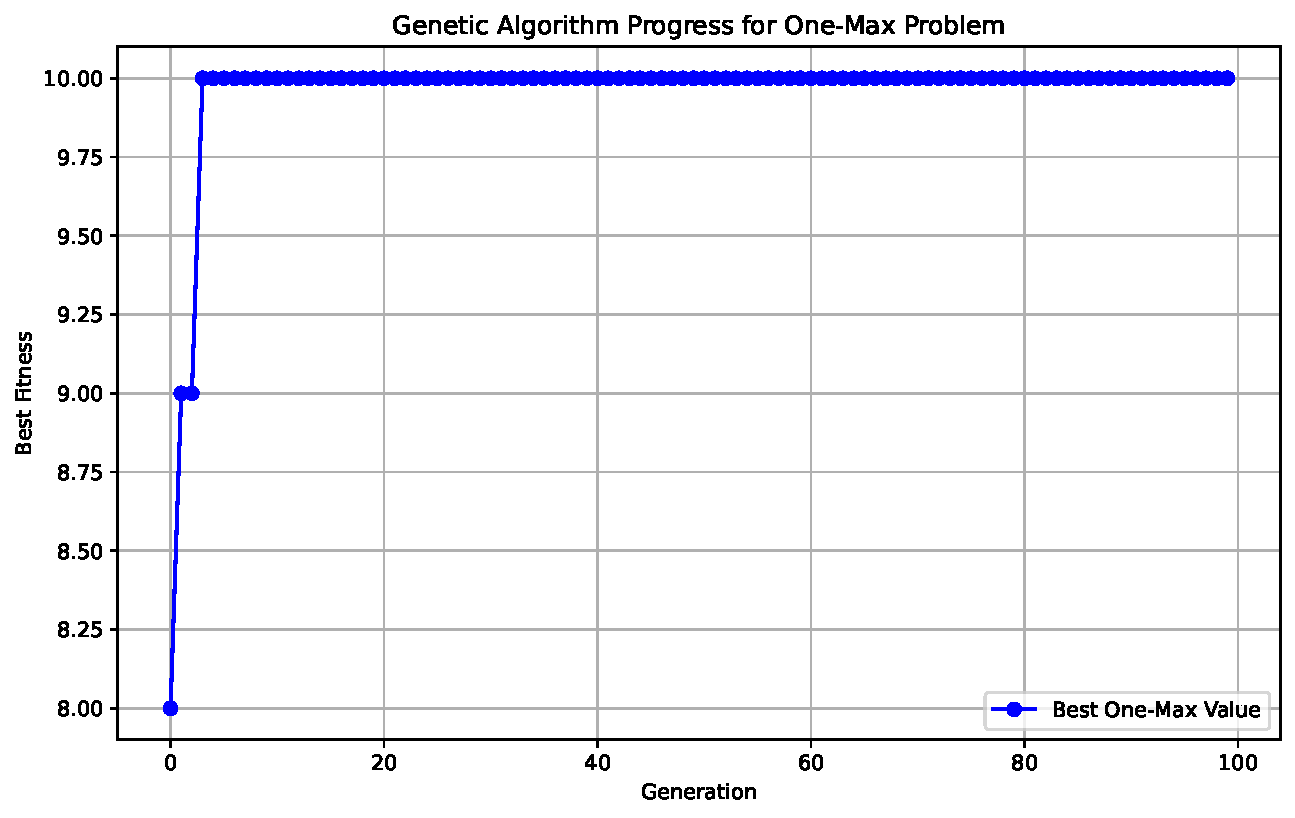
\includegraphics[keepaspectratio]{es_files/figure-pdf/cell-12-output-2.pdf}}

\begin{itemize}
\tightlist
\item
  Overall, the output confirms the accuracy and efficiency of the search
  in this specific case, identifying the minimum accurately in a very
  short time.
\item
  Optimal x: The search identified \(x=0\) as the value that minimizes
  the Ackley function at 0. Since the Ackley function's global minimum
  is known to occur at zero (specifically, at \(x=0\) for each input
  variable), this result confirms the function's minimum in this search.
\item
  Optimal value: This is the computed minimum value of the Ackley
  function at \(x=0\). This very small number, so close to zero but
  slightly above due to computational limitations or floating-point
  precision. It's effectively zero for practical purposes, indicating
  the function reached its theoretical minimum.
\item
  Execution time: 0.002003 seconds -- The exhaustive search took just
  over 2 milliseconds to complete. This quick time suggests that the
  search was likely performed in a low-dimensional space (such as 1D or
  2D), where an exhaustive approach can be executed efficiently. In
  higher dimensions, exhaustive search would generally take
  significantly longer due to the exponential increase in the number of
  points to evaluate.
\end{itemize}

\bookmarksetup{startatroot}

\chapter{Comparing One Max to Ackley}\label{comparing-one-max-to-ackley}

\begin{itemize}
\tightlist
\item
  Initialization() Function: In an exhaustive search on the Ackley
  function, a step size is essential because the Ackley function
  operates in a continuous space, meaning the variables can take any
  real value within a defined range. The step size determines the
  resolution of the search, dictating how closely spaced the evaluation
  points are. A finer step size means more precise exploration of the
  function's landscape, potentially identifying the global minimum more
  accurately, but at the cost of increased computation. Without a
  defined step size, exhaustive search would theoretically require an
  infinite number of evaluations, as there are infinitely many points in
  a continuous space. In contrast, the One Max problem typically
  operates in a discrete binary space (e.g., binary strings), where each
  variable can only take values of 0 or 1. This structure doesn't
  require a step size, as all possible solutions are already discrete
  and finite. Each solution is a unique binary string, and the
  exhaustive search simply evaluates every possible string without
  needing to subdivide the space further.
\item
  Transition() Function: In the Ackley function, when you define a
  function like \(T(s, idx, x_values)\) and use return
  x\_values{[}idx{]}, you are treating the search space as a continuous
  or discretized array of possible values. Here, x\_values is typically
  a list or array containing the potential values for each variable
  dimension, and idx simply indexes into this array to retrieve a
  specific value. Since exhaustive search involves systematically
  testing all possible values in x\_values, there's no need for
  incremental addition \((s += 1)\); instead, the function directly
  retrieves the next possible value at a given index, which is common in
  continuous or multi-valued spaces. In contrast, the One Max problem is
  a binary optimization problem where the goal is to maximize the sum of
  binary values (0s and 1s). The search space consists of binary strings
  rather than a continuous or finely discretized set. Incrementing \(s\)
  (like \(s += 1\)) in this context might be used to iterate over binary
  configurations or to shift values systematically, as each
  configuration can only be either a 0 or a 1. This incremental approach
  is necessary in One Max because there is no list of predefined values
  (like x\_values); rather, each binary position in the solution must be
  systematically altered to generate each possible solution.
\item
  Evaluation() Function: E(v) in the Ackley function evaluates
  continuous real values for minimization, while bin(s).count(``1'') in
  the One Max problem evaluates binary integers for maximization. A
  lower evaluation result from E(v) indicates a better solution in terms
  of proximity to the global minimum while a higher count of ``1''s in
  bin(s).count(``1'') represents a better solution, as it means the
  solution is closer to the optimal binary string of all 1s.
\item
  Determine() Function: In one max, we want to maximize. In Ackley, we
  want to minimize. This affects the determination function: if f\_v
  \textless{} f\_s (for minimize) vs f\_v \textgreater{} f\_s (for
  maximize)
\end{itemize}

\bookmarksetup{startatroot}

\chapter{Using AI}\label{using-ai-4}

\begin{itemize}
\tightlist
\item
  Use the following prompt on a generative AI, like chatGPT, to learn
  more about the topics covered.
\item
  Concept of Exhaustive Search: Explain, in your own words, what an
  exhaustive search is and how it systematically explores all possible
  solutions. Why is this method guaranteed to find the optimal solution?
\item
  Advantages and Limitations: Discuss the advantages and disadvantages
  of using exhaustive search for solving optimization problems. When
  would you avoid using it?
\item
  Comparison with Heuristics: Compare exhaustive search with heuristic
  methods (like greedy algorithms). When would you prioritize optimality
  over computational efficiency?
\item
  Greedy vs.~Exhaustive: Reflect on a problem where you would
  instinctively use a greedy approach but later realize an exhaustive
  search would yield a better result. What changed your decision?
\item
  Continuous vs Discrete Domains: Discuss how exhaustive search differs
  when applied to continuous domains (e.g., Ackley function) versus
  discrete domains (e.g., knapsack problem). Why does step size matter
  in continuous optimization?
\item
  Trade-Offs in Optimization: Reflect on a scenario where exhaustive
  search would be impractical. How would you modify the problem or
  approach to make it solvable within reasonable time and resources?
\item
  Visualization Insights: How does visualizing the search process (e.g.,
  fitness evolution over time) help in understanding and debugging
  optimization algorithms?
\end{itemize}

\bookmarksetup{startatroot}

\chapter{Conclusions}\label{conclusions-3}

\begin{itemize}
\tightlist
\item
  Choose exhaustive search for small-scale problems where optimality is
  critical. Use heuristics for large, complex, or high-dimensional
  spaces.
\end{itemize}

\bookmarksetup{startatroot}

\chapter{Hill Climbing}\label{hill-climbing}

\bookmarksetup{startatroot}

\chapter{Hill Climbing (HC)}\label{hill-climbing-hc}

\begin{itemize}
\item
  If life is like hill climbing, what's the moment where you took a
  single small step that ended up leading you to your biggest peak?
\item
  Hill Climbing is an optimization algorithm that starts with an
  arbitrary solution to a problem and iteratively makes small changes to
  the solution, choosing the change that improves the solution the most.
\item
  Characteristics

  \begin{itemize}
  \tightlist
  \item
    Greedy Approach: It selects the most promising neighboring solution
    based on the heuristic, or it uses a search strategy that is to
    accept only a better solution as the next solution.
  \item
    Local Search: Only considers the local neighborhood of the current
    solution. This implies that if there are local optima located
    between the initial solution and the optimal solution, HC may get
    stuck at a local optimum.
  \item
    Termination: Ends when no further improvements can be made.
  \end{itemize}
\item
  Applications: Used in various fields like AI for game playing,
  pathfinding, and scheduling problems.
\end{itemize}

\section{Search Strategy of HC
\textgreater{}}\label{search-strategy-of-hc}

\begin{itemize}
\tightlist
\item
  The search strategy of HC that accepts only a better solution as the
  next solution.
\item
  Suppose HC has a 50/50 chance to move either left or right in solving
  the one-max problem; then, in addition to the global optimum (1111),
  HC may end up in one of the seven or three local optima.
  \(f(v)>f(s)\).
\end{itemize}

\begin{figure}[H]

{\centering \pandocbounded{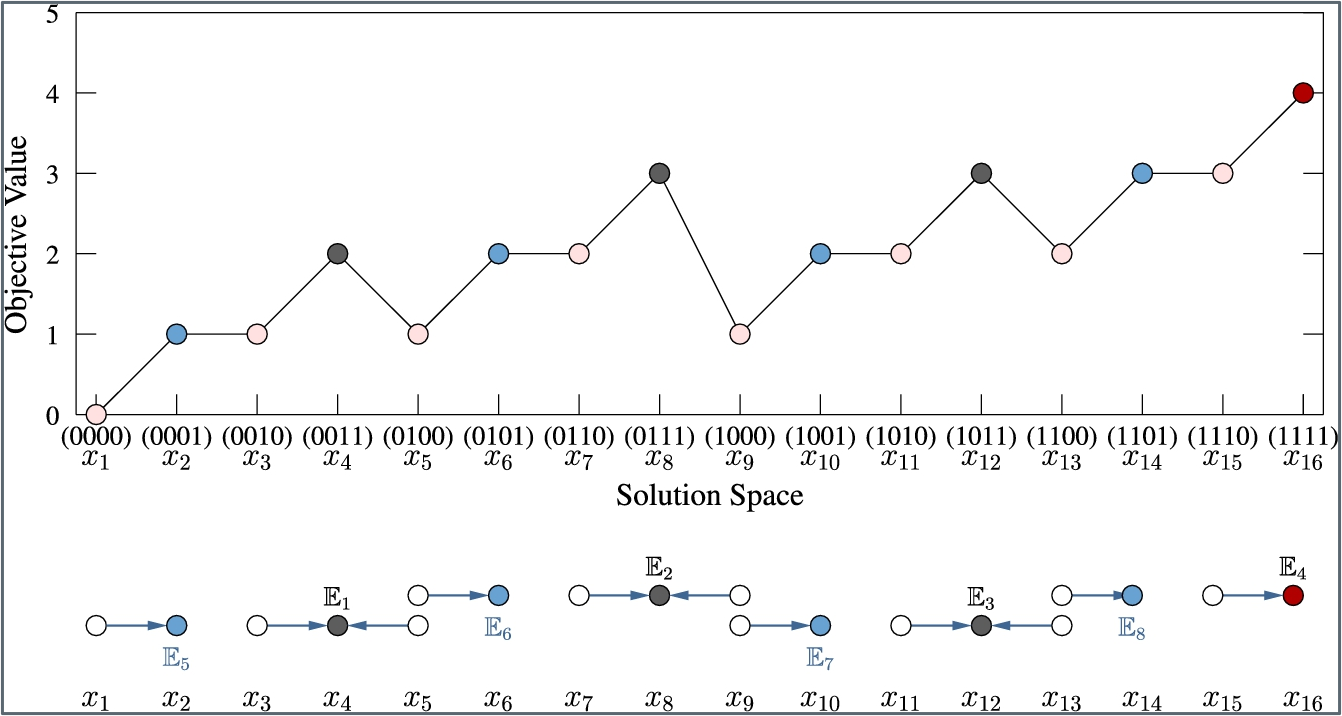
\includegraphics[keepaspectratio]{Pictures/hc.png}}

}

\caption{hc search}

\end{figure}%

\section{Search Strategy of HC
\textgreater=}\label{search-strategy-of-hc-1}

\begin{itemize}
\tightlist
\item
  The search strategy of HC accepts both better solutions and solutions
  that are equally good as the next solution.
\item
  The possible result if HC accepts not only a better solution but also
  a solution that is equally good (i.e., \(f(v)>=f(s)\) as the next
  solution; then only the solutions \(x_4\) \((0011)\), \(x_8\)
  \((0111)\), and \(x_12\) \((1011)\) will remain as the local optima,
  while \(x_16\) \((1111)\) is the global optimum.
\end{itemize}

\begin{figure}[H]

{\centering \pandocbounded{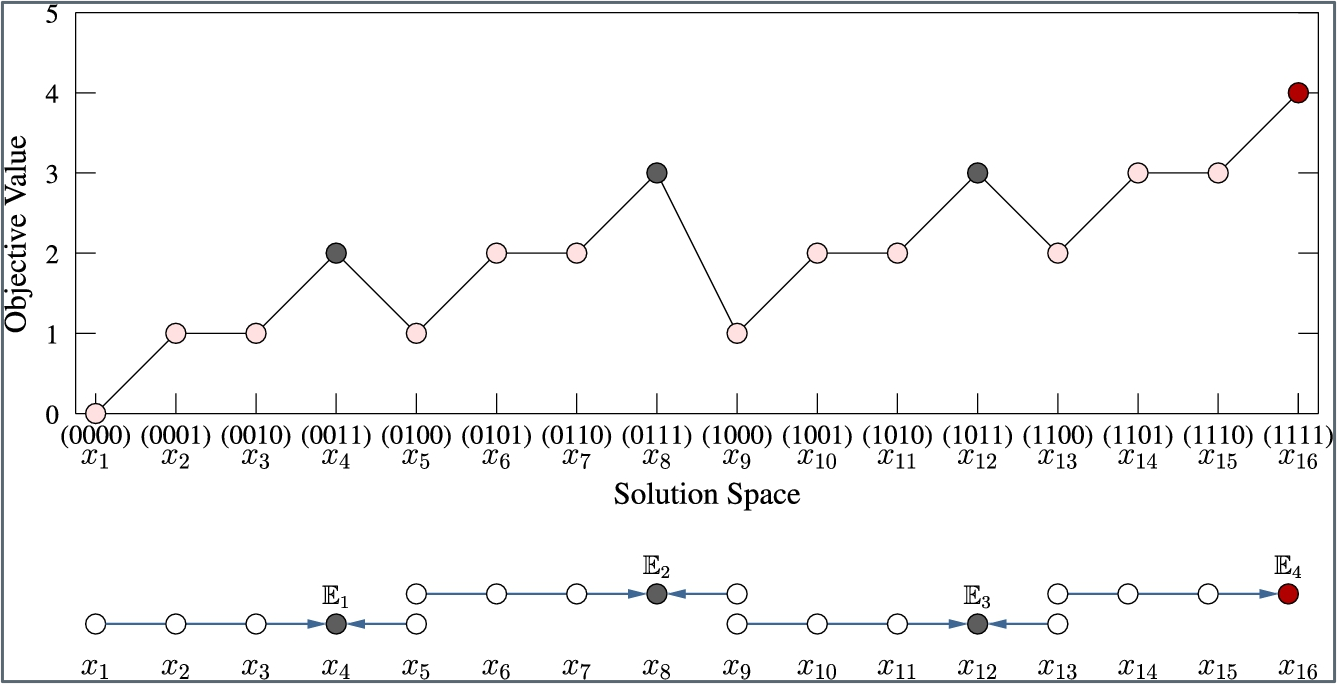
\includegraphics[keepaspectratio]{Pictures/hc2.png}}

}

\caption{hc search}

\end{figure}%

\section{Hill Climbing Algorithm}\label{hill-climbing-algorithm}

\begin{itemize}
\tightlist
\item
  Start: Initialize with a random solution or a predefined starting
  point.
\item
  Evaluate: Assess the quality of the current solution using a heuristic
  function.
\item
  Generate Neighbors: Produce a set of neighboring solutions by making
  small changes.
\item
  Select Best Neighbor: Choose the neighbor that has the highest
  heuristic value.
\item
  Move: Replace the current solution with the selected neighbor.
\item
  Repeat: Continue the process until no better neighbors are found or a
  stopping criterion is met.
\end{itemize}

\begin{figure}[H]

{\centering \pandocbounded{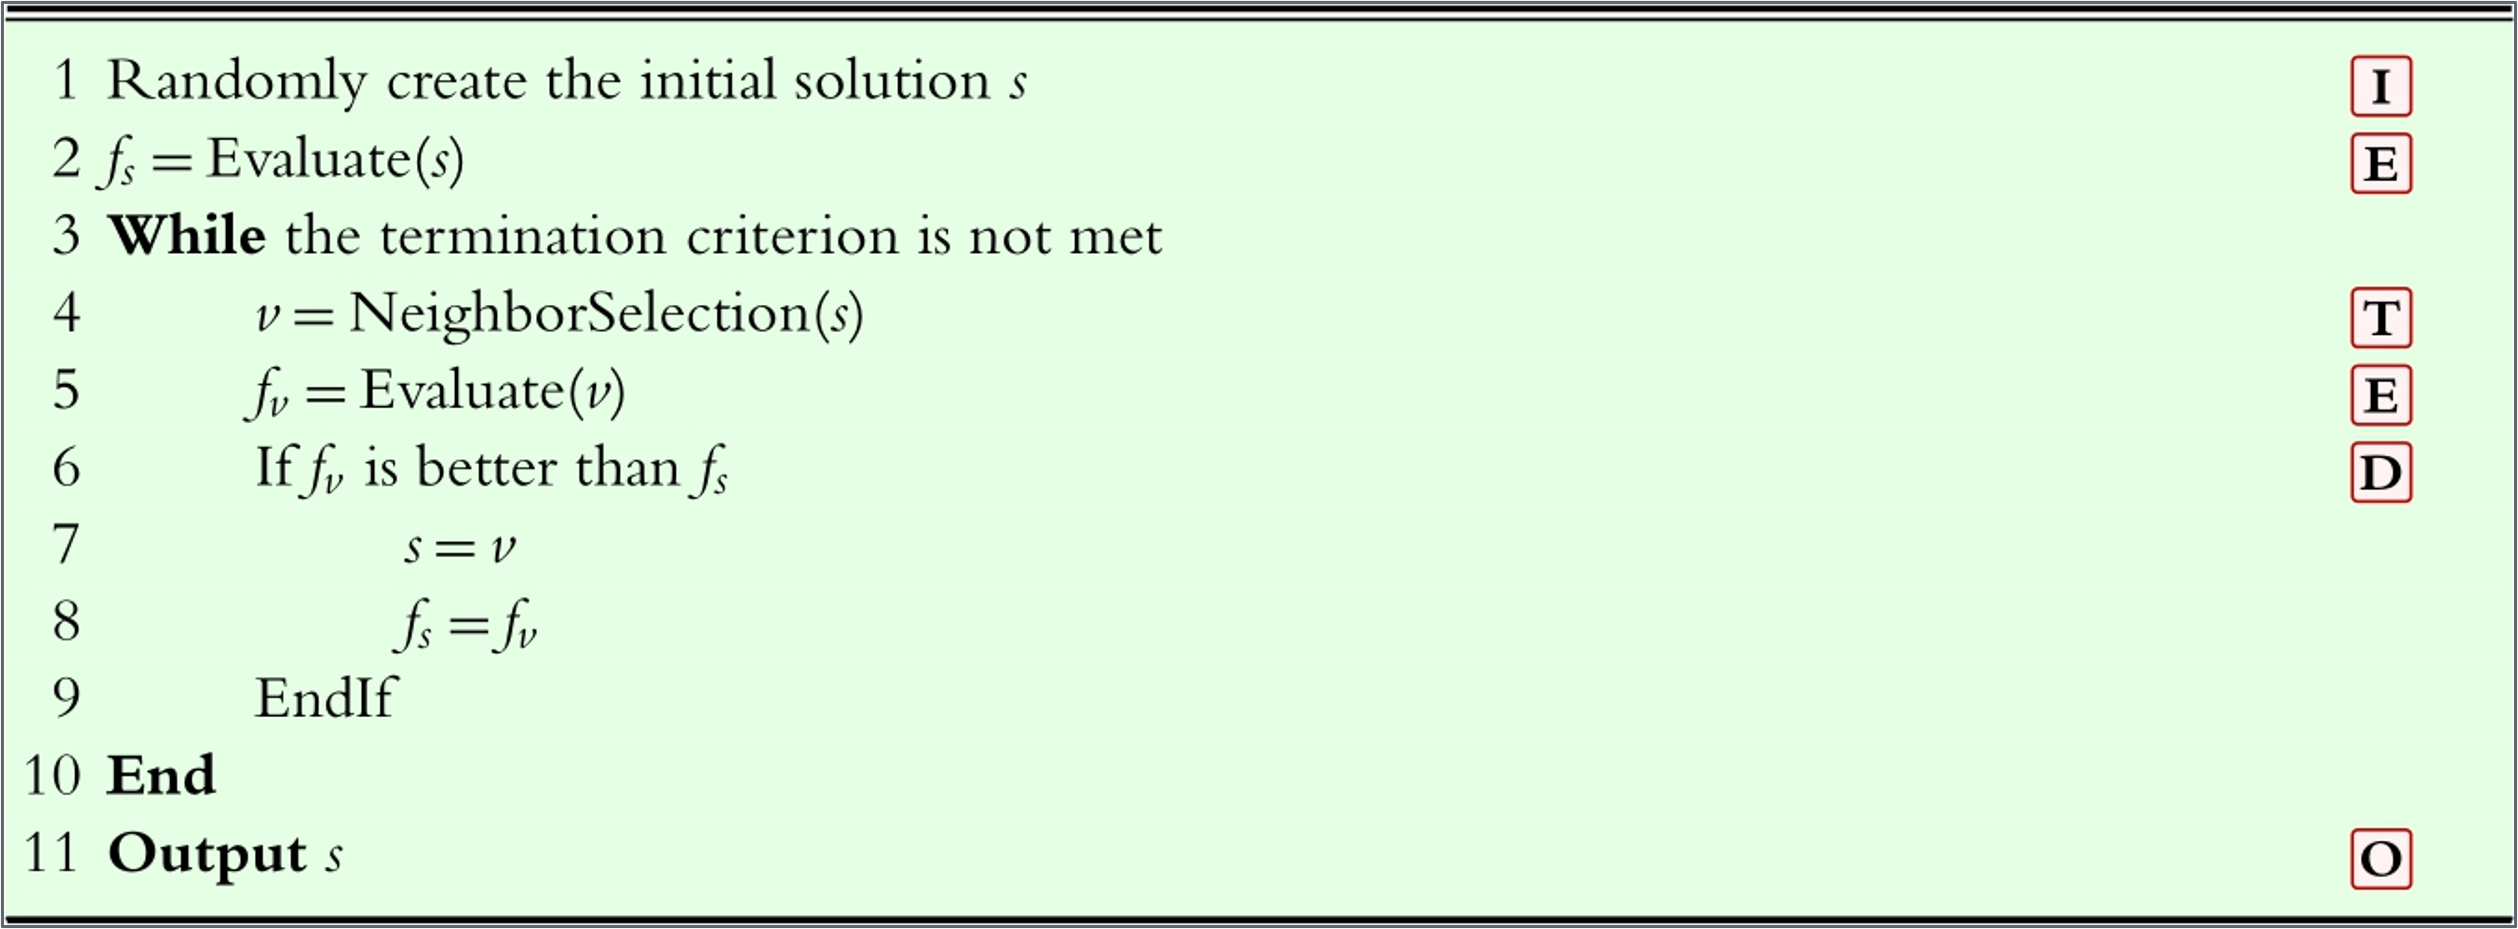
\includegraphics[keepaspectratio]{Pictures/hc3.png}}

}

\caption{hc algo}

\end{figure}%

\section{Challenges of HC}\label{challenges-of-hc}

\begin{itemize}
\item
  Local Maximum: Hill climbing may get stuck at a local maximum, where
  no neighboring solution improves, but better solutions exist further
  away.
\item
  Plateaus: It can struggle on flat regions where no clear direction of
  improvement is evident.
\item
  Ridges: Difficulties in navigating narrow ridges that require moving
  sideways to find a better peak.
\item
  Variations to Overcome Limitations

  \begin{itemize}
  \tightlist
  \item
    Stochastic Hill Climbing: Introduces randomness to avoid local
    maxima.
  \item
    Simulated Annealing: Uses probabilistic decisions to escape local
    maxima and explore a larger solution space.
  \item
    Steepest-Ascent Hill Climbing: Considers all neighbors and selects
    the one with the steepest ascent.
  \end{itemize}
\end{itemize}

\bookmarksetup{startatroot}

\chapter{Program for One Max
Implementation}\label{program-for-one-max-implementation}

\begin{itemize}
\tightlist
\item
  Import necessary tools: time for timing and matplotlib for plotting
  results.
\end{itemize}

\begin{Shaded}
\begin{Highlighting}[]
\ImportTok{import}\NormalTok{ numpy }\ImportTok{as}\NormalTok{ np}
\ImportTok{import}\NormalTok{ time}
\ImportTok{import}\NormalTok{ matplotlib.pyplot }\ImportTok{as}\NormalTok{ plt}
\end{Highlighting}
\end{Shaded}

\begin{itemize}
\tightlist
\item
  Set num\_bits equal to a number (10) in this case.
\end{itemize}

\begin{Shaded}
\begin{Highlighting}[]
\NormalTok{num\_bits }\OperatorTok{=} \DecValTok{10}  \CommentTok{\# You can adjust the number of bits}
\end{Highlighting}
\end{Shaded}

\section{Set up Run Function}\label{set-up-run-function}

\begin{itemize}
\tightlist
\item
  Evaluate the initial solution by counting the number of 1s, which
  serves as the ``fitness'' value.
\item
  Search for Neighbors: Generate neighboring solutions by flipping one
  bit at a time in the current solution. For each neighbor, calculate
  its fitness (number of 1s in its binary representation).
\item
  Select Best Neighbor: Identify the neighboring solution with the
  highest fitness.If this neighbor's fitness is better than the current
  solution's fitness, update the current solution to this neighbor.
\item
  Repeat Until Convergence: Continue generating and evaluating neighbors
  until no neighboring solution improves the current fitness (local
  maximum reached).Track the fitness of the best solution at each
  iteration for plotting or analysis.
\item
  Return Best Solution and Fitness Progress: Output the best solution
  found along with a list of fitness values over iterations.
\end{itemize}

\begin{Shaded}
\begin{Highlighting}[]
\CommentTok{\# Run function for hill climbing}
\KeywordTok{def}\NormalTok{ run\_hc(num\_bits}\OperatorTok{=}\DecValTok{10}\NormalTok{, max\_evals}\OperatorTok{=}\DecValTok{2} \OperatorTok{**}\NormalTok{ num\_bits):}
\NormalTok{    sol }\OperatorTok{=}\NormalTok{ init\_hc(num\_bits)  }\CommentTok{\# Initialize random solution}
\NormalTok{    fitness }\OperatorTok{=}\NormalTok{ evaluate(sol)  }\CommentTok{\# Evaluate the initial solution}
\NormalTok{    fitness\_over\_time }\OperatorTok{=}\NormalTok{ []}
    
\NormalTok{    eval\_count }\OperatorTok{=} \DecValTok{0}

    \CommentTok{\# Main loop of evaluations}
    \ControlFlowTok{while}\NormalTok{ eval\_count }\OperatorTok{\textless{}}\NormalTok{ max\_evals:}
\NormalTok{        tmp\_sol }\OperatorTok{=}\NormalTok{ transit(sol)  }\CommentTok{\# Make a random change (flip a bit)}
\NormalTok{        tmp\_fitness }\OperatorTok{=}\NormalTok{ evaluate(tmp\_sol)  }\CommentTok{\# Evaluate the new solution}
\NormalTok{        sol, fitness }\OperatorTok{=}\NormalTok{ determine(tmp\_sol, tmp\_fitness, sol, fitness)  }\CommentTok{\# Determine if we accept the new solution}
        
\NormalTok{        fitness\_over\_time.append(fitness)  }\CommentTok{\# Track the fitness over time}
\NormalTok{        eval\_count }\OperatorTok{+=} \DecValTok{1}
        
    \ControlFlowTok{return}\NormalTok{ fitness\_over\_time, sol}
\end{Highlighting}
\end{Shaded}

\section{Helper Functions:}\label{helper-functions-1}

\begin{itemize}
\tightlist
\item
  Initiate: Set Initial Solution: Randomly choose an initial binary
  solution of the specified bit length (num\_bits).
\end{itemize}

\begin{Shaded}
\begin{Highlighting}[]
\CommentTok{\# Function for initialization (I)}
\KeywordTok{def}\NormalTok{ init\_hc(num\_bits):}
    \ControlFlowTok{return}\NormalTok{ np.random.randint(}\DecValTok{2}\NormalTok{, size}\OperatorTok{=}\NormalTok{num\_bits, dtype}\OperatorTok{=}\BuiltInTok{int}\NormalTok{)}
\end{Highlighting}
\end{Shaded}

\begin{itemize}
\tightlist
\item
  Transit (Generate Neighbors): Create a function that generates all
  neighbors of a binary solution by flipping each bit one by one.
\end{itemize}

\begin{Shaded}
\begin{Highlighting}[]
\CommentTok{\# Function for transit: (T) }
\CommentTok{\# Flipping a random bit in the solution}
\KeywordTok{def}\NormalTok{ transit(sol):}
\NormalTok{    new\_sol }\OperatorTok{=}\NormalTok{ sol.copy()}
\NormalTok{    flip\_index }\OperatorTok{=}\NormalTok{ np.random.randint(}\BuiltInTok{len}\NormalTok{(sol))}
\NormalTok{    new\_sol[flip\_index] }\OperatorTok{=} \DecValTok{1} \OperatorTok{{-}}\NormalTok{ new\_sol[flip\_index]  }\CommentTok{\# Flip the bit (0 to 1, or 1 to 0)}
    \ControlFlowTok{return}\NormalTok{ new\_sol}
\end{Highlighting}
\end{Shaded}

\begin{itemize}
\tightlist
\item
  Evaluate: Count the number of 1s in the binary representation of a
  solution (fitness value).
\end{itemize}

\begin{Shaded}
\begin{Highlighting}[]
\CommentTok{\# Function for evaluation: (E) }
\CommentTok{\# Sum the number of 1s (OneMax problem)}
\KeywordTok{def}\NormalTok{ evaluate(sol):}
    \ControlFlowTok{return}\NormalTok{ np.}\BuiltInTok{sum}\NormalTok{(sol)}
\end{Highlighting}
\end{Shaded}

\begin{itemize}
\tightlist
\item
  Determine: Track and update the current best solution and its fitness
  as the search progresses.
\end{itemize}

\begin{Shaded}
\begin{Highlighting}[]
\CommentTok{\# Function for determine: (D) }
\CommentTok{\# Decide whether to accept the new solution}
\KeywordTok{def}\NormalTok{ determine(tmp\_sol, tmp\_fitness, sol, fitness):}
    \ControlFlowTok{if}\NormalTok{ tmp\_fitness }\OperatorTok{\textgreater{}}\NormalTok{ fitness:}
        \ControlFlowTok{return}\NormalTok{ tmp\_sol, tmp\_fitness  }\CommentTok{\# Accept the new solution}
    \ControlFlowTok{return}\NormalTok{ sol, fitness  }\CommentTok{\# Keep the current solution}
\end{Highlighting}
\end{Shaded}

\begin{itemize}
\tightlist
\item
  The main execution section initiates the hill climbing algorithm,
  recording the time taken to execute it. It captures the progression of
  fitness values over each iteration and identifies the best solution
  found, while calculating the total execution time.
\end{itemize}

\begin{Shaded}
\begin{Highlighting}[]
\CommentTok{\# Main Execution}
\CommentTok{\# Run hill climbing and get fitness values}
\NormalTok{start\_time }\OperatorTok{=}\NormalTok{ time.time()}
\NormalTok{fitness\_over\_time, best\_solution }\OperatorTok{=}\NormalTok{ run\_hc(num\_bits)}
\NormalTok{end\_time }\OperatorTok{=}\NormalTok{ time.time()}
\NormalTok{execution\_time }\OperatorTok{=}\NormalTok{ end\_time }\OperatorTok{{-}}\NormalTok{ start\_time  }\CommentTok{\# Calculate elapsed time}
\end{Highlighting}
\end{Shaded}

\begin{itemize}
\tightlist
\item
  The output section displays key details about the hill climbing
  algorithm, including its name, the number of bits used, and the time
  taken for execution. It then visualizes the fitness evolution across
  evaluations, providing a clear plot that shows how fitness values
  change over time as the algorithm progresses toward the best solution.
\end{itemize}

\begin{Shaded}
\begin{Highlighting}[]
\CommentTok{\# Output and visualize}
\BuiltInTok{print}\NormalTok{(}\SpecialStringTok{f"\# Name of the search algorithm: Hill Climbing"}\NormalTok{)}
\BuiltInTok{print}\NormalTok{(}\SpecialStringTok{f"\# number of bits: }\SpecialCharTok{\{}\NormalTok{num\_bits}\SpecialCharTok{\}}\SpecialStringTok{"}\NormalTok{)}
\BuiltInTok{print}\NormalTok{(}\SpecialStringTok{f"Time elapsed: }\SpecialCharTok{\{}\NormalTok{execution\_time}\SpecialCharTok{:.6f\}}\SpecialStringTok{ seconds"}\NormalTok{)  }\CommentTok{\# Print the elapsed time}

\CommentTok{\# Plot the evolution of fitness over time}
\NormalTok{plt.figure(figsize}\OperatorTok{=}\NormalTok{(}\DecValTok{10}\NormalTok{, }\DecValTok{6}\NormalTok{))}
\NormalTok{plt.plot(fitness\_over\_time, label}\OperatorTok{=}\StringTok{\textquotesingle{}Fitness over time\textquotesingle{}}\NormalTok{, color}\OperatorTok{=}\StringTok{\textquotesingle{}blue\textquotesingle{}}\NormalTok{, linewidth}\OperatorTok{=}\DecValTok{2}\NormalTok{)}
\NormalTok{plt.title(}\SpecialStringTok{f\textquotesingle{}Hill Climbing: Fitness Evolution (}\SpecialCharTok{\{}\NormalTok{num\_bits}\SpecialCharTok{\}}\SpecialStringTok{ bits)\textquotesingle{}}\NormalTok{)}
\NormalTok{plt.xlabel(}\StringTok{\textquotesingle{}Evaluations\textquotesingle{}}\NormalTok{)}
\NormalTok{plt.ylabel(}\StringTok{\textquotesingle{}Fitness (Number of 1s)\textquotesingle{}}\NormalTok{)}
\NormalTok{plt.grid(}\VariableTok{True}\NormalTok{)}
\NormalTok{plt.legend()}
\NormalTok{plt.show()}
\end{Highlighting}
\end{Shaded}

\begin{verbatim}
# Name of the search algorithm: Hill Climbing
# number of bits: 10
Time elapsed: 0.008999 seconds
\end{verbatim}

\pandocbounded{\includegraphics[keepaspectratio]{hc_files/figure-pdf/cell-10-output-2.pdf}}

\begin{itemize}
\tightlist
\item
  In the chart above, the fitness score, which measures the number of 1s
  in a 10-bit solution, is shown over a series of evaluations.
  Initially, the fitness rapidly increases, suggesting that the hill
  climbing algorithm quickly finds improvements in the solution. Once it
  reaches the maximum fitness of 10, it stabilizes and remains flat,
  indicating that the algorithm has found an optimal solution and no
  further improvements are being made.
\end{itemize}

\section{\texorpdfstring{Comparison of ES and HC for the one-max Problem
of size
\(n=10\)}{Comparison of ES and HC for the one-max Problem of size n=10}}\label{comparison-of-es-and-hc-for-the-one-max-problem-of-size-n10}

\begin{itemize}
\tightlist
\item
  HC-LR and HC-Rand to denote a similar thing. HC-Rand and HC-LR differ
  primarily in how they choose the next solution and handle exploration,
  impacting their likelihood of getting stuck in local optima.
\item
  HC-LR (Hill Climbing with Limited Range): HC-LR's transition operator
  restricts it to move only to adjacent solutions, which makes it less
  flexible. The solution v of HC-LR will be the one that is one smaller
  or one larger than the current solution s (i.e., \(v=s−1\) or
  \(v=s+1\)). As described in the example, if HC-LR starts with the
  solution ``1000,'' it can only move to ``0111'' or ``1001.'' If
  neither of these options provides an improvement, HC-LR is likely to
  get stuck there, leading to a local optimum. Because HC-LR only
  accepts moves that improve the solution, it has a high risk of getting
  trapped in suboptimal points without exploring further.
\item
  HC-Rand (Hill Climbing with Randomization): HC-Rand randomly selects a
  part of the current solution to invert, allowing it to explore a
  broader range of possible next solutions. This random approach reduces
  the chance of getting stuck in a local optimum since the algorithm has
  the flexibility to try different options, even if they are not
  immediately better. HC-Rand's randomness increases the probability of
  escaping local optima, thus improving the chances of finding a global
  optimum.

  \begin{itemize}
  \tightlist
  \item
    The solution v of HC-Rand will be created by inverting a randomly
    chosen subsolution of s (i.e., ``1'' becomes ``0'' and ``0'' becomes
    ``1''). The transition operator in the HC-Rand (Hill Climbing with
    Randomization) algorithm randomly selects a part (subsolution) of
    the current solution and inverts the chosen bit(s). For a ``one-max
    problem'' of a specific size (where the goal is to maximize the
    number of 1s in the solution), inverting different bits can produce
    several possible next solutions.
  \item
    In the example given, there are four possible new solutions because
    there are four different bits that could be inverted from the
    current solution. If inverting one bit doesn't improve the objective
    value (e.g., the number of 1s), HC-Rand will consider other options,
    allowing it to avoid getting stuck in local optima. This random
    inversion helps HC-Rand explore other solutions, increasing the
    chances of finding the global maximum (an optimal solution with the
    highest number of 1s).
  \end{itemize}
\item
  In both cases, only a better solution will be accepted as the next
  solution \(v\).
\end{itemize}

\begin{figure}[H]

{\centering \pandocbounded{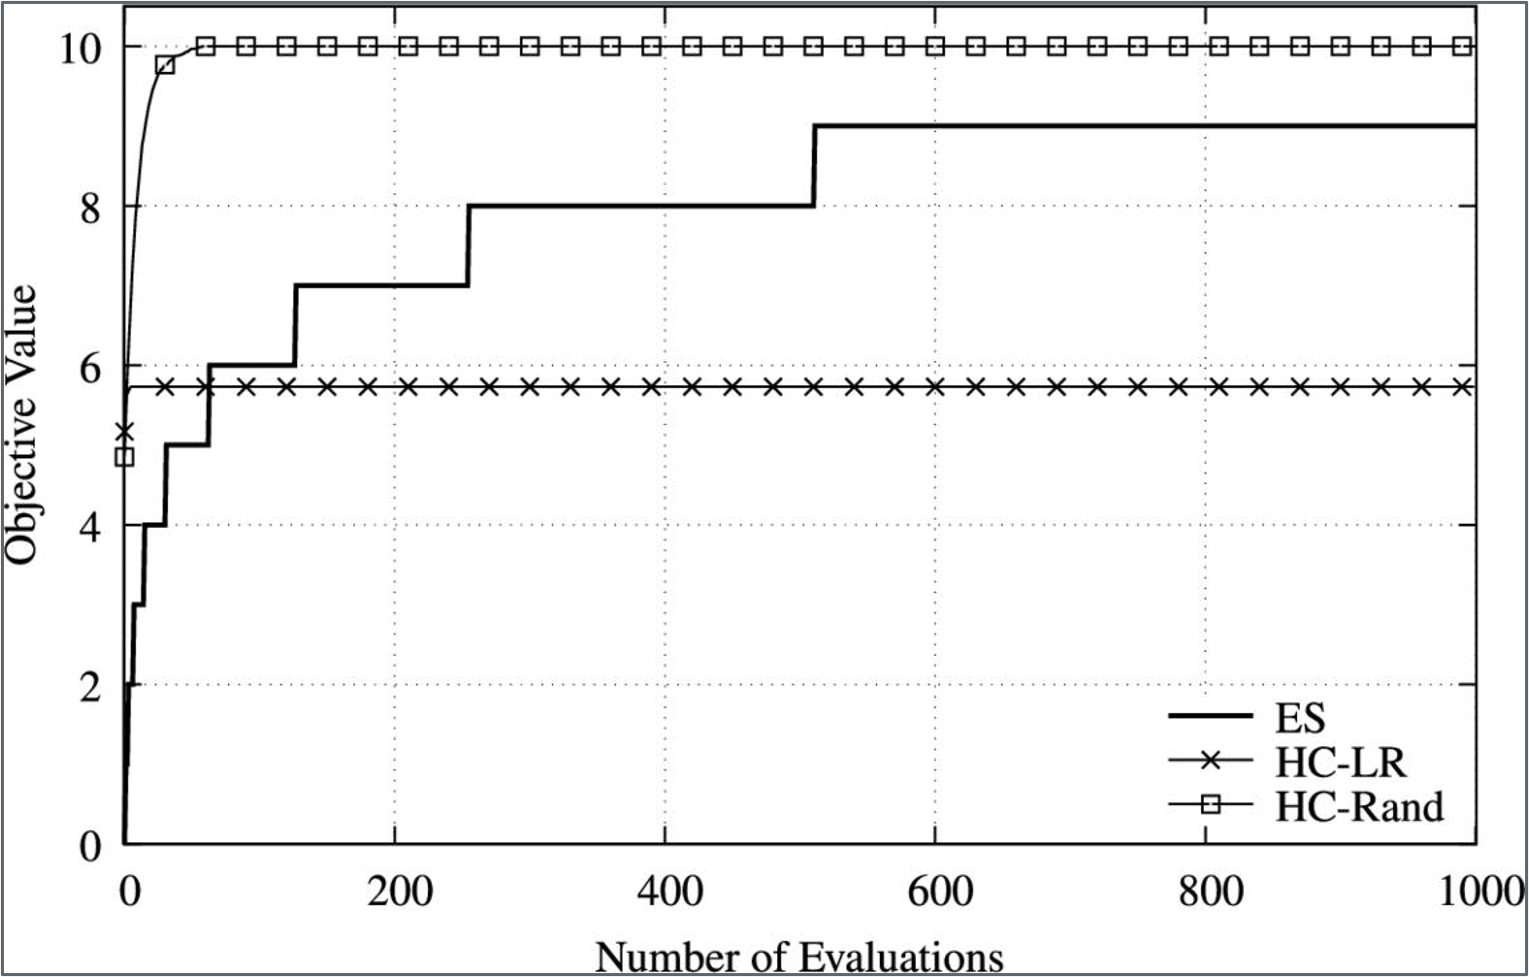
\includegraphics[keepaspectratio]{Pictures/hcRand.png}}

}

\caption{hc search}

\end{figure}%

\bookmarksetup{startatroot}

\chapter{Search strategy}\label{search-strategy}

\begin{itemize}
\tightlist
\item
  The Search Strategy of HC-Rand when Starting from the Candidate
  Solution \(x_9\)
\item
  HC-LR will then move to either \(x_8\) \((0111)\) or \(x_9\)
  \((1001)\) in this case and eventually get stuck there.
\item
  HC-Rand has a chance to find the global optimum \(x_16\) because the
  next possible solutions of \(x_13\) \((1100)\) will be \(x_5\)
  \((0100)\), \(x_9\) \((1000)\), \(x_15\) \((1110)\), and \(x_14\)
  \((1101)\).
\end{itemize}

\begin{figure}[H]

{\centering \pandocbounded{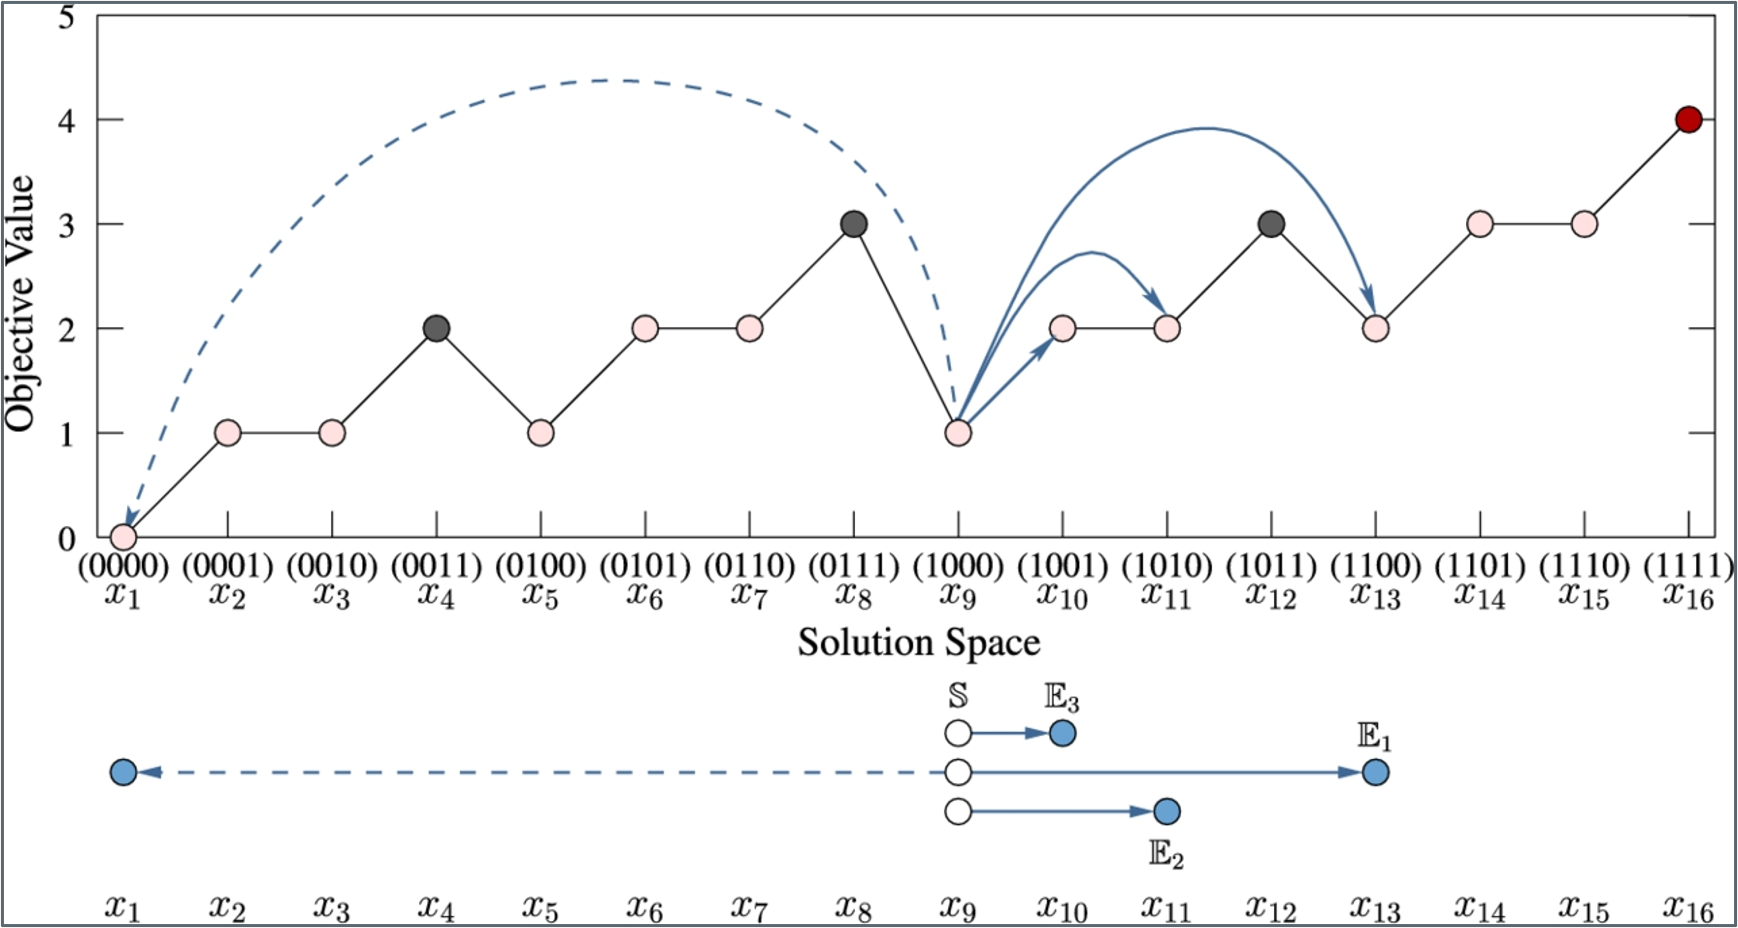
\includegraphics[keepaspectratio]{Pictures/hc4.png}}

}

\caption{hc search}

\end{figure}%

\begin{itemize}
\item
  Simulation Results of HC for a Deceptive Problem of size \(n=4\)
\item
  The results show that ES is able to find the optimal solution quickly,
  because only 16 checks (evaluations) are needed, for there are in
  total 16 candidate solutions in this case.
\item
  The results also show that HC-LR is unable to find the optimal
  solution sometimes when applying it to an optimization problem that
  has one or more local optima, even if the trap is not that complex.
  \pandocbounded{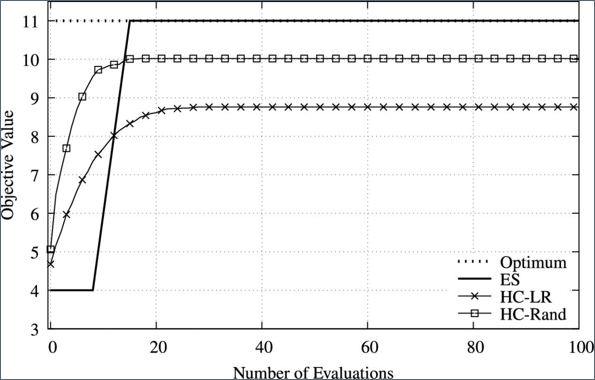
\includegraphics[keepaspectratio]{Pictures/hc5.png}}
\item
  Simulation Results of HC for a Deceptive Problem of size \(n=10\)
\item
  The number of evaluations ES requires to find the optimal solution
  increases significantly. In this case, ES is unable to find the
  optimal solution within 1000 evaluations.
\item
  It is reasonable to expect that ES will take 1024 evaluations to find
  the optimal solution because it has to check all possible candidate
  solutions, and with \(n=10\) there are exactly \(2^n=2^10=1024\)
  possible candidate solutions.
\item
  These results show that both HC-based algorithms are able to find a
  better result than ES at the early stage of the convergence process. *
  This implies that HC provides an alternative way to find an
  approximate solution for large and complex optimization problems.
\end{itemize}

\begin{figure}[H]

{\centering \pandocbounded{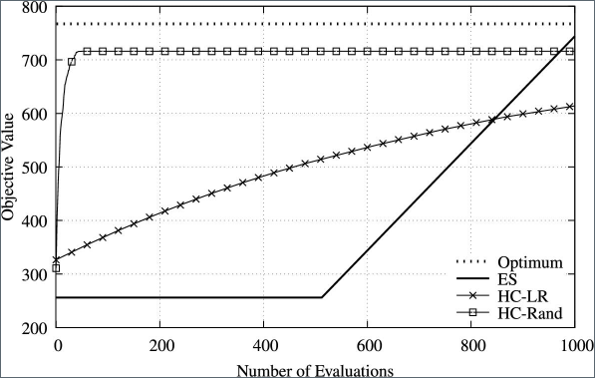
\includegraphics[keepaspectratio]{Pictures/hc6.png}}

}

\caption{hc search}

\end{figure}%

\begin{itemize}
\tightlist
\item
  The Search Strategy of ES for the BSD-2 Problem of size \(n = 4\)
\item
  Assuming that the starting point is the solution \(x_5\) \((0100)\).
  The next solution will then be \(x_13\), \(x_1\), \(x_7\), or \(x_6\).
  This implies that HC-Rand has a good chance to move to a solution in
  the region \(x_6-x_16\).
\item
  The probability of moving to the left region \(x_1-x_4\) or the right
  region \(x_6-x_16\) depends somehow on the location of the current
  solution.
\item
  A move to the right region is a guarantee to find the optimal
  solution, and a move to the left region is destined to a local optimum
  in this case.
\end{itemize}

\begin{figure}[H]

{\centering \pandocbounded{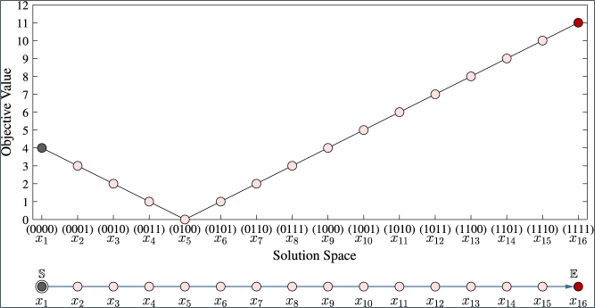
\includegraphics[keepaspectratio]{Pictures/hc7.png}}

}

\caption{hc search}

\end{figure}%

\begin{itemize}
\tightlist
\item
  The Search Strategy of HC-LR for the BSD-2 Problem of size \(n=4\)
\item
  The search strategy of HC-LR makes it possible to either get stuck at
  the local optimum \(x_1\) or find the global optimum \(x_16\),
  depending on the starting point.
\item
  If the starting point is in the range \(x_1-x_4\), HC-LR will
  certainly end up getting stuck at the local optimum \(x_1\).
\item
  If the starting point is in the range \(x_6-x_16\), HC-LR will surely
  end up finding the optimal solution.
\item
  If HC-LR starts with the solution \(x_5\), it has a 50/50 chance to
  get stuck at the local optimum or to find the global optimum.
\item
  The probability for HC-LR to get stuck at the local optimum \(x_1\) is
  4/16 + .5/16 = 4.5/16. 4/16 represents the probability of reaching
  \(x_1\) directly from other states or due to the structure of the
  search space. 0.5/16: This small additional probability could
  represent an edge case, such as when the algorithm gets ``trapped'' in
  \(x_1\) due to a random restart condition or slight chance of stopping
  early.
\item
  The probability for it to find the global optimum \(x_16\) is 11/16 +
  .5/16 =11.5/16. 11/16 represents the probability of reaching \(x_16\),
  potentially due to the structure of the search space and favorable
  transitions, while 0.5/16 could be an additional small probability for
  reaching \(x_16\) due to a random factor, such as a random restart
  helping the algorithm reach the global optimum.
\end{itemize}

\begin{figure}[H]

{\centering \pandocbounded{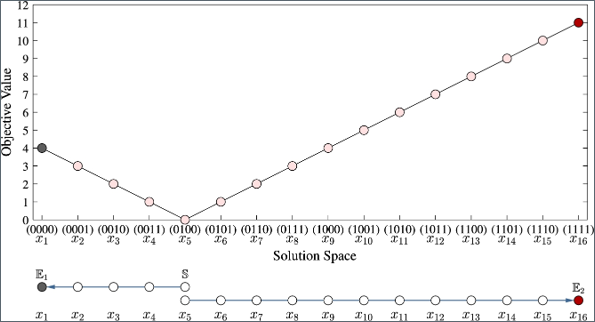
\includegraphics[keepaspectratio]{Pictures/hc8.png}}

}

\caption{hc search}

\end{figure}%

\begin{itemize}
\tightlist
\item
  The Search Strategy of HC-Rand for a Deceptive Problem of size
  \(n=4\).
\item
  Assuming that the starting point is the solution \(x_5\) \((0100)\).
  The next solution will then be \(x_13\), \(x_1\), \(x_7\), or \(x_6\).
\item
  This implies that HC-Rand has a good chance to move to a solution in
  the region \(x_6-x_16\). The probability of moving to the left region
  \(x_1-x_4\) or the right region \(x_6-x_16\) depends somehow on the
  location of the current solution. A move to the right region is a
  guarantee to find the optimal solution, and a move to the left region
  is destined to a local optimum in this case.
\end{itemize}

\begin{figure}[H]

{\centering \pandocbounded{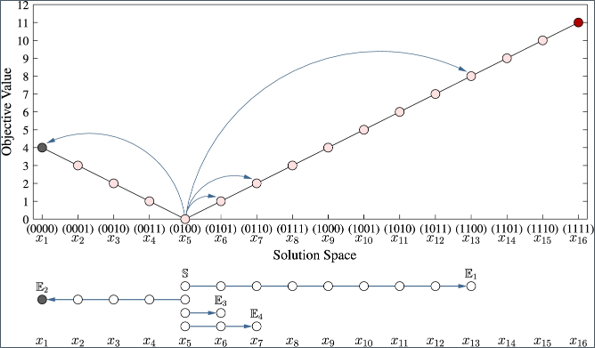
\includegraphics[keepaspectratio]{Pictures/hc9.png}}

}

\caption{hc search}

\end{figure}%

\section{Deciphering Probability of
Switching}\label{deciphering-probability-of-switching}

\begin{itemize}
\item
  The landscape of the ``solution space'' or ``search space'' of an
  optimization problem seen by a search can be different when:

  \begin{itemize}
  \tightlist
  \item
    different ways are used to represent the solutions or
  \item
    different ways are used to generate new candidate solutions from
    current solutions.
  \end{itemize}
\item
  The solution space that a search algorithm sees can also be called the
  ``search space.''
\item
  HC-Rand-M: If we use ``\textgreater='' instead of ``\textgreater{}''
  in the comparison of the current solution and the possible next
  solution for solving the BSD-2 problem of sizes n=4 and n=10.
\item
  The results of HC-Rand-M show that with this modification, HC-Rand
  will be able to find the optimal solution in most cases.
\end{itemize}

\begin{figure}[H]

{\centering \pandocbounded{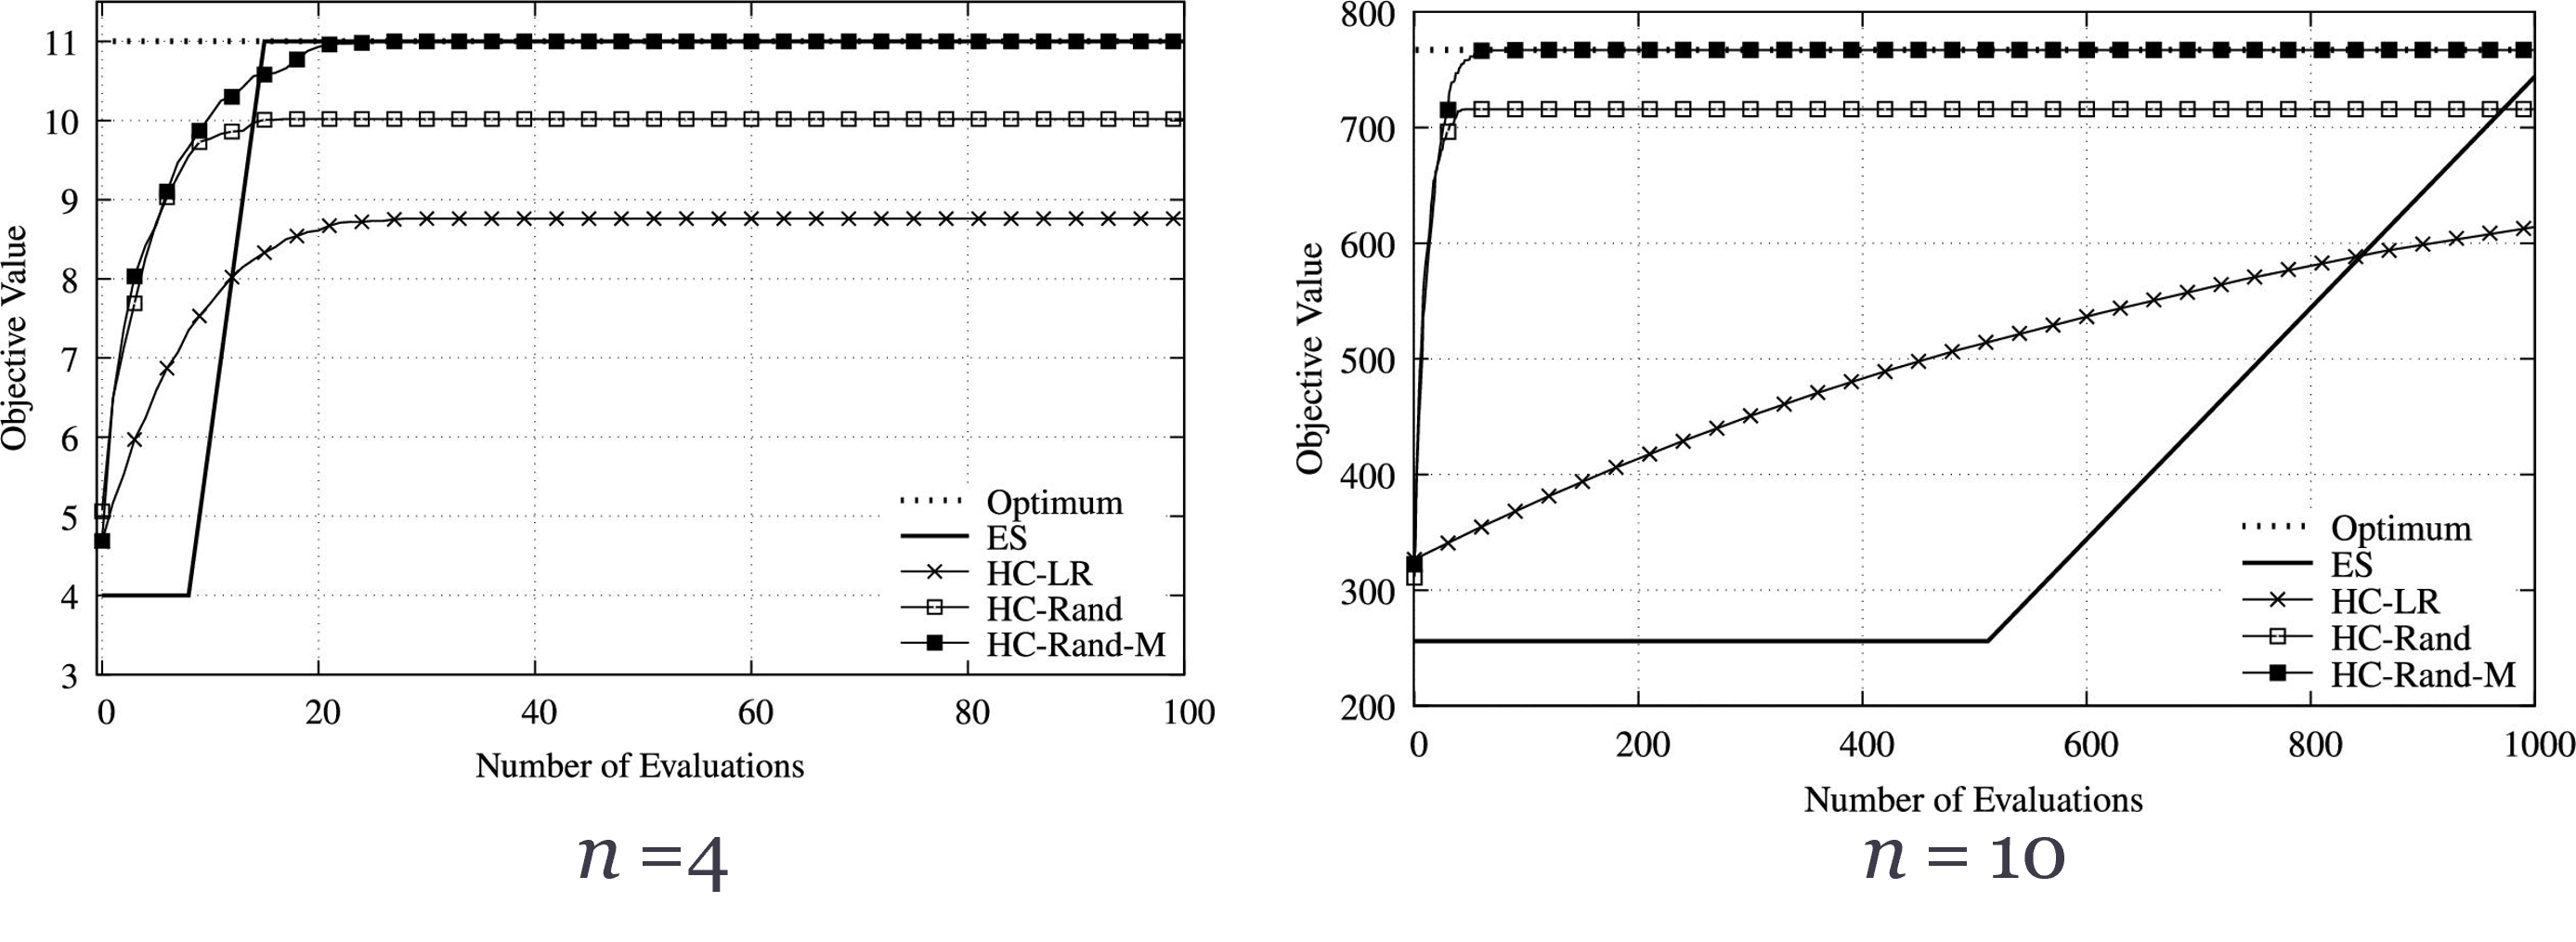
\includegraphics[keepaspectratio]{Pictures/hc10.png}}

}

\caption{hc search}

\end{figure}%

\bookmarksetup{startatroot}

\chapter{Hill Climbing using Ackley
Function}\label{hill-climbing-using-ackley-function}

\begin{itemize}
\tightlist
\item
  A Hill Climbing algorithm designed to optimize the given func (in this
  case the Ackley function).
\item
  Ackley(x): This is the function we want to optimize.
\item
  hill\_climbing(): This function performs the optimization.

  \begin{itemize}
  \tightlist
  \item
    start: The initial point or guess where the algorithm begins.
  \item
    step\_size: The distance to move left or right from the current
    position to generate new candidate solutions. Commonly used
    step\_size values depend on the specific problem scale and the shape
    of the Ackley function.
  \item
    max\_iterations: The maximum number of iterations to perform,
    ensuring the algorithm eventually stops if no local maximum is found
    before this limit.

    \begin{itemize}
    \tightlist
    \item
      Limit on the number of iterations to avoid infinite loops.
    \end{itemize}
  \end{itemize}
\item
  At each step, the algorithm compares the current solution to its
  neighbors (by moving left or right by step\_size) and picks the better
  one.
\item
  The process stops when no better neighbors are found (local maximum).
\end{itemize}

\section{Load Imports}\label{load-imports}

\begin{Shaded}
\begin{Highlighting}[]
\ImportTok{import}\NormalTok{ numpy }\ImportTok{as}\NormalTok{ np}
\ImportTok{import}\NormalTok{ time}
\ImportTok{import}\NormalTok{ random}
\ImportTok{import}\NormalTok{ matplotlib.pyplot }\ImportTok{as}\NormalTok{ plt}

\NormalTok{np.random.seed(}\DecValTok{5042}\NormalTok{) }\CommentTok{\#\#for consistency}
\end{Highlighting}
\end{Shaded}

\section{Define the Ackley Function
(1D)}\label{define-the-ackley-function-1d}

\begin{itemize}
\tightlist
\item
  Function f(x): This is the function we want to optimize.
\item
  In this case, Ackley function with provided formula.
\end{itemize}

\begin{Shaded}
\begin{Highlighting}[]
\CommentTok{\# Ackley function in 1D}
\KeywordTok{def}\NormalTok{ ackley(x):}
\NormalTok{    a }\OperatorTok{=} \DecValTok{20}
\NormalTok{    b }\OperatorTok{=} \FloatTok{0.2}
\NormalTok{    c }\OperatorTok{=} \DecValTok{2} \OperatorTok{*}\NormalTok{ np.pi}
\NormalTok{    term1 }\OperatorTok{=} \OperatorTok{{-}}\NormalTok{a }\OperatorTok{*}\NormalTok{ np.exp(}\OperatorTok{{-}}\NormalTok{b }\OperatorTok{*}\NormalTok{ np.sqrt(np.mean(np.square(x))))}
\NormalTok{    term2 }\OperatorTok{=} \OperatorTok{{-}}\NormalTok{np.exp(np.mean(np.cos(c }\OperatorTok{*}\NormalTok{ np.array(x))))}
    \ControlFlowTok{return}\NormalTok{ term1 }\OperatorTok{+}\NormalTok{ term2 }\OperatorTok{+}\NormalTok{ a }\OperatorTok{+}\NormalTok{ np.exp(}\DecValTok{1}\NormalTok{)}
\end{Highlighting}
\end{Shaded}

\section{Main Loop}\label{main-loop-1}

\begin{itemize}
\tightlist
\item
  This is where the hill climbing algorithm repeatedly evaluates
  candidate solutions, compares them with the current solution, and
  decides whether to update the current solution. This loop is crucial
  because it drives the optimization process by iterating over a fixed
  number of steps or until a stopping criterion is met.
\item
  The current solution is set to start\_x, which was initialized
  earlier. The Ackley value for this starting solution is calculated and
  stored in current\_value.x\_history and value\_history keep track of
  all the solutions and function values (fitness) encountered during the
  optimization process.
\item
  The hill climbing loop runs for a fixed number of iterations
  (max\_iters), which controls how many optimization steps are
  performed. Each iteration represents one optimization step, where two
  new candidate solutions are generated and evaluated.
\item
  The transit function generates two neighboring solutions, left\_x and
  right\_x, by subtracting and adding the step\_size (0.1 by default) to
  the current solution (current\_x). These represent potential moves to
  the left and right in the search space.
\item
  Both neighboring solutions are evaluated using the Ackley function,
  resulting in their corresponding values (left\_value and
  right\_value). These values represent how ``good'' the new solutions
  are (lower is better in this minimization problem). Then we compare
  all three solutions (current, left, and right).

  \begin{itemize}
  \tightlist
  \item
    The np.argmin(values) function finds the index of the minimum value
    (best solution) from the three candidates.
  \item
    The determine function then decides whether to update the current
    solution (current\_x) to the new best solution.
  \end{itemize}
\item
  The current solution and its corresponding function value are appended
  to the history lists (x\_history and value\_history). These lists will
  be used later to plot the progress of the algorithm.
\item
  Finally, we return the results.
\end{itemize}

\begin{Shaded}
\begin{Highlighting}[]
\CommentTok{\# Main hill climbing loop for Ackley function in 1D}
\KeywordTok{def}\NormalTok{ hill\_climbing\_ackley(start\_x, max\_iters}\OperatorTok{=}\DecValTok{100}\NormalTok{, step\_size}\OperatorTok{=}\FloatTok{0.1}\NormalTok{):}
\NormalTok{    current\_x }\OperatorTok{=}\NormalTok{ start\_x}
\NormalTok{    current\_value }\OperatorTok{=}\NormalTok{ evaluate(current\_x)}
\NormalTok{    x\_history }\OperatorTok{=}\NormalTok{ [current\_x]}
\NormalTok{    value\_history }\OperatorTok{=}\NormalTok{ [current\_value]}

    \ControlFlowTok{for}\NormalTok{ \_ }\KeywordTok{in} \BuiltInTok{range}\NormalTok{(max\_iters):}
\NormalTok{        left\_x, right\_x }\OperatorTok{=}\NormalTok{ transit(current\_x, step\_size)}
\NormalTok{        left\_value }\OperatorTok{=}\NormalTok{ evaluate(left\_x)}
\NormalTok{        right\_value }\OperatorTok{=}\NormalTok{ evaluate(right\_x)}

\NormalTok{        values }\OperatorTok{=}\NormalTok{ [current\_value, left\_value, right\_value]}
\NormalTok{        x\_candidates }\OperatorTok{=}\NormalTok{ [current\_x, left\_x, right\_x]}

\NormalTok{        best\_index }\OperatorTok{=}\NormalTok{ np.argmin(values)}
\NormalTok{        current\_x, current\_value }\OperatorTok{=}\NormalTok{ determine(values[best\_index], current\_value, x\_candidates[best\_index], current\_x)}

\NormalTok{        x\_history.append(current\_x)}
\NormalTok{        value\_history.append(current\_value)}

    \ControlFlowTok{return}\NormalTok{ current\_x, current\_value, x\_history, value\_history}
\end{Highlighting}
\end{Shaded}

\section{Helper Functions}\label{helper-functions-2}

\begin{itemize}
\tightlist
\item
  Initialize: This function initializes the hill climbing process by
  selecting a random starting point (start\_x) within the given range
  {[}-10, 10{]}. This represents the initial solution that hill climbing
  will start with.
\end{itemize}

\begin{Shaded}
\begin{Highlighting}[]
\CommentTok{\# Initialization function (I) to set the starting point}
\KeywordTok{def}\NormalTok{ init\_hc(range\_min}\OperatorTok{={-}}\DecValTok{10}\NormalTok{, range\_max}\OperatorTok{=}\DecValTok{10}\NormalTok{):}
    \ControlFlowTok{return}\NormalTok{ random.uniform(range\_min, range\_max)}
\end{Highlighting}
\end{Shaded}

\begin{itemize}
\tightlist
\item
  Transition: This function generates two new candidate solutions by
  taking small steps (of size 0.1) to the left and right of the current
  solution (current\_x). These represent possible transitions to
  neighboring points in the search space.
\end{itemize}

\begin{Shaded}
\begin{Highlighting}[]
\CommentTok{\# Transition function (T)}
\KeywordTok{def}\NormalTok{ transit(current\_x, step\_size}\OperatorTok{=}\FloatTok{0.1}\NormalTok{):}
    \ControlFlowTok{return}\NormalTok{ current\_x }\OperatorTok{{-}}\NormalTok{ step\_size, current\_x }\OperatorTok{+}\NormalTok{ step\_size}
\end{Highlighting}
\end{Shaded}

\begin{itemize}
\tightlist
\item
  Evaluation: This function evaluates the fitness of a solution (sol)
  using the Ackley function. The goal of the hill climbing algorithm is
  to minimize this value. The Ackley function is typically used for
  testing optimization algorithms due to its complex landscape with many
  local minima.
\end{itemize}

\begin{Shaded}
\begin{Highlighting}[]
\CommentTok{\# Evaluation function (E) to evaluate fitness (Ackley value in this case)}
\KeywordTok{def}\NormalTok{ evaluate(sol):}
    \ControlFlowTok{return}\NormalTok{ ackley([sol])}
\end{Highlighting}
\end{Shaded}

\begin{itemize}
\tightlist
\item
  Determination: This function compares the current solution's value
  (current\_value) with the value of a new candidate solution
  (new\_value). If the new solution is better (i.e., has a lower Ackley
  value), it becomes the new current solution. Otherwise, the current
  solution is retained.
\end{itemize}

\begin{Shaded}
\begin{Highlighting}[]
\CommentTok{\# Determination (D)}
\CommentTok{\# Function to decide whether to accept the new solution}
\KeywordTok{def}\NormalTok{ determine(new\_value, current\_value, new\_x, current\_x):}
    \ControlFlowTok{return}\NormalTok{ (new\_x, new\_value) }\ControlFlowTok{if}\NormalTok{ new\_value }\OperatorTok{\textless{}}\NormalTok{ current\_value }\ControlFlowTok{else}\NormalTok{ (current\_x, current\_value)}
\end{Highlighting}
\end{Shaded}

\section{Main Execution}\label{main-execution-1}

\begin{itemize}
\tightlist
\item
  The process starts by initializing start\_x using the Initialization
  function (init\_hc). The main function (hill\_climbing\_ackley) then
  runs for a fixed number of iterations (100 by default) using
  Transition to generate candidate solutions, Evaluation to evaluate
  them, and Determination to decide whetherr to accept a new solution.
\end{itemize}

\begin{Shaded}
\begin{Highlighting}[]
\CommentTok{\# Main execution}
\NormalTok{start\_x }\OperatorTok{=}\NormalTok{ init\_hc()}
\NormalTok{start\_time }\OperatorTok{=}\NormalTok{ time.time()}
\NormalTok{optimal\_x, optimal\_value, x\_history, value\_history }\OperatorTok{=}\NormalTok{ hill\_climbing\_ackley(start\_x)}
\NormalTok{end\_time }\OperatorTok{=}\NormalTok{ time.time()}
\NormalTok{execution\_time }\OperatorTok{=}\NormalTok{ end\_time }\OperatorTok{{-}}\NormalTok{ start\_time}
\end{Highlighting}
\end{Shaded}

\section{Output}\label{output-1}

\begin{itemize}
\tightlist
\item
  The first part prints the optimal solution found (optimal\_x), the
  corresponding function value (optimal\_value), and the total time
  taken for the execution.
\item
  The second part plots the Ackley function over the range {[}-10, 10{]}
  and overlays the hill climbing progress. The points in red represent
  the steps taken by the hill climbing algorithm as it navigates through
  the search space.
\end{itemize}

\begin{Shaded}
\begin{Highlighting}[]
\CommentTok{\# Output (O)}
\BuiltInTok{print}\NormalTok{(}\SpecialStringTok{f"Optimal x: }\SpecialCharTok{\{}\NormalTok{optimal\_x}\SpecialCharTok{\}}\SpecialStringTok{"}\NormalTok{)}
\BuiltInTok{print}\NormalTok{(}\SpecialStringTok{f"Optimal value: }\SpecialCharTok{\{}\NormalTok{optimal\_value}\SpecialCharTok{\}}\SpecialStringTok{"}\NormalTok{)}
\BuiltInTok{print}\NormalTok{(}\SpecialStringTok{f"Execution time: }\SpecialCharTok{\{}\NormalTok{execution\_time}\SpecialCharTok{:.6f\}}\SpecialStringTok{ seconds"}\NormalTok{)}


\CommentTok{\# Plot the Ackley function and hill climbing progress}
\NormalTok{x\_range }\OperatorTok{=}\NormalTok{ np.linspace(}\OperatorTok{{-}}\DecValTok{10}\NormalTok{, }\DecValTok{10}\NormalTok{, }\DecValTok{1000}\NormalTok{)}
\NormalTok{y\_values }\OperatorTok{=}\NormalTok{ [ackley([x]) }\ControlFlowTok{for}\NormalTok{ x }\KeywordTok{in}\NormalTok{ x\_range]}

\NormalTok{plt.plot(x\_range, y\_values, label}\OperatorTok{=}\StringTok{"Ackley Function"}\NormalTok{)}
\NormalTok{plt.plot(x\_history, value\_history, }\StringTok{\textquotesingle{}ro{-}{-}\textquotesingle{}}\NormalTok{, label}\OperatorTok{=}\StringTok{"Hill Climbing Progress"}\NormalTok{)}
\NormalTok{plt.xlabel(}\StringTok{"x"}\NormalTok{)}
\NormalTok{plt.ylabel(}\StringTok{"f(x)"}\NormalTok{)}
\NormalTok{plt.title(}\StringTok{"Hill Climbing on Ackley Function in 1D"}\NormalTok{)}
\NormalTok{plt.legend()}
\NormalTok{plt.grid(}\VariableTok{True}\NormalTok{)}
\NormalTok{plt.show()}
\end{Highlighting}
\end{Shaded}

\begin{verbatim}
Optimal x: -3.9973379295354587
Optimal value: 11.0090150716548
Execution time: 0.002999 seconds
\end{verbatim}

\pandocbounded{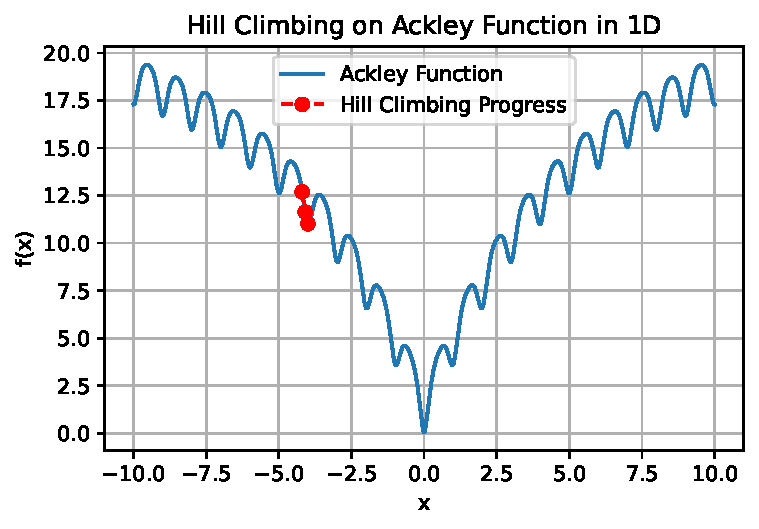
\includegraphics[keepaspectratio]{hc_files/figure-pdf/cell-19-output-2.pdf}}

\begin{itemize}
\tightlist
\item
  An example run of this put the points Optimal x: 5.03 and Optimal
  Value: 12.75, are suboptimal for the Ackley function.
\item
  For the Ackley function in 1D, the global minimum occurs at \(x=0\),
  and the function value at this point is exactly \(f(0)=0\).
\item
  Our results are not close to the global minimum of \(x=0\). Any value
  greater than zero indicates that the algorithm has not found the true
  global minimum.
\item
  The blue line represents the Ackley function over a range of \(x\)
  values from -10 to 10.The red dots connected by dashed lines represent
  the progress of the hill climbing algorithm as it iterates through
  neighboring solutions.
\item
  The Ackley function is known for its many local minima, and hill
  climbing is a greedy optimization method that tends to get stuck in
  local minima because it only moves to the immediate best neighboring
  solution. Once it finds a local minimum, it stops, even if it hasn't
  found the global minimum.
\item
  In this case, the result you obtained is a local minimum but not the
  global minimum. Since \(f(0)=0\) is the global minimum, and your
  result is \(f(5.03)= 12.75\), the algorithm likely got stuck in a
  local minimum during its search.
\item
  Simulated Annealing is a more advanced version of hill climbing that
  sometimes accepts worse solutions to escape local optima. Will discuss
  later.
\end{itemize}

\bookmarksetup{startatroot}

\chapter{Hill Climbing with Finance}\label{hill-climbing-with-finance}

\begin{itemize}
\item
  Diversifying your stock portfolio?
\item
  The Sharpe Ratio is formula measures the performance of an investment
  compared to a risk-free asset, after adjusting for risk.
\item
  The higher the Sharpe ratio, the better the risk-adjusted performance.
  \(S\) is the Sharpe Ratio \(R_p\) is the expected return of the
  portfolio, \(R_f\) is the risk-free rate of return, \(\sigma_p\) is
  the standard deviation (volatility) of the portfolio's excess return.
  \(S = \frac{R_p - R_f}{\sigma_p}\)
\item
  We store the Sharpe ratio at each successful iteration in
  score\_history, which allows us to plot the progress of the Sharpe
  ratio over time.
\item
  This performance function calculates the Sharpe ratio based on the
  portfolio weights, daily returns, and the covariance matrix of the
  assets.
\item
  The weights are normalized (sum to 1) both when generating the initial
  random portfolio and for the neighboring portfolio in each iteration.
\item
  The code prints the best portfolio weights and the best Sharpe ratio
  found after the hill climbing process. The plot will show the
  improvement in the Sharpe ratio during the iterations.
\end{itemize}

\section{Imports}\label{imports-1}

\begin{Shaded}
\begin{Highlighting}[]
\CommentTok{\#\# Hill Climbing Finance example}
\ImportTok{import}\NormalTok{ yfinance }\ImportTok{as}\NormalTok{ yf}
\ImportTok{import}\NormalTok{ numpy }\ImportTok{as}\NormalTok{ np}
\ImportTok{import}\NormalTok{ pandas }\ImportTok{as}\NormalTok{ pd}
\ImportTok{import}\NormalTok{ matplotlib.pyplot }\ImportTok{as}\NormalTok{ plt}
\ImportTok{import}\NormalTok{ time}

\NormalTok{np.random.seed(}\DecValTok{5042}\NormalTok{)}
\end{Highlighting}
\end{Shaded}

\section{Fetching Data}\label{fetching-data}

\begin{Shaded}
\begin{Highlighting}[]
\NormalTok{stocks }\OperatorTok{=}\NormalTok{ [}\StringTok{\textquotesingle{}AAPL\textquotesingle{}}\NormalTok{, }\StringTok{\textquotesingle{}GOOGL\textquotesingle{}}\NormalTok{, }\StringTok{\textquotesingle{}MSFT\textquotesingle{}}\NormalTok{, }\StringTok{\textquotesingle{}AMZN\textquotesingle{}}\NormalTok{, }\StringTok{\textquotesingle{}TSLA\textquotesingle{}}\NormalTok{, }\StringTok{\textquotesingle{}NFLX\textquotesingle{}}\NormalTok{, }\StringTok{\textquotesingle{}NVDA\textquotesingle{}}\NormalTok{, }\StringTok{\textquotesingle{}META\textquotesingle{}}\NormalTok{, }\StringTok{\textquotesingle{}DIS\textquotesingle{}}\NormalTok{, }\StringTok{\textquotesingle{}BA\textquotesingle{}}\NormalTok{] }
\NormalTok{start\_date }\OperatorTok{=} \StringTok{\textquotesingle{}2023{-}10{-}01\textquotesingle{}}
\NormalTok{end\_date }\OperatorTok{=} \StringTok{\textquotesingle{}2024{-}10{-}1\textquotesingle{}}

\CommentTok{\# Fetch historical stock data}
\KeywordTok{def}\NormalTok{ fetch\_data(stocks, start\_date, end\_date):}
\NormalTok{    data }\OperatorTok{=}\NormalTok{ yf.download(stocks, start}\OperatorTok{=}\NormalTok{start\_date, end}\OperatorTok{=}\NormalTok{end\_date)[}\StringTok{\textquotesingle{}Adj Close\textquotesingle{}}\NormalTok{]}
    \ControlFlowTok{return}\NormalTok{ data}
\end{Highlighting}
\end{Shaded}

\section{Calculating performance via Sharpe
Ratio}\label{calculating-performance-via-sharpe-ratio}

\begin{Shaded}
\begin{Highlighting}[]
\CommentTok{\# Calculate portfolio performance (returns, risk, and Sharpe ratio)}
\KeywordTok{def}\NormalTok{ portfolio\_performance(weights, mean\_returns, cov\_matrix):}
\NormalTok{    returns }\OperatorTok{=}\NormalTok{ np.}\BuiltInTok{sum}\NormalTok{(mean\_returns }\OperatorTok{*}\NormalTok{ weights) }\OperatorTok{*} \DecValTok{252}  \CommentTok{\# Annualized returns}
\NormalTok{    risk }\OperatorTok{=}\NormalTok{ np.sqrt(np.dot(weights.T, np.dot(cov\_matrix, weights))) }\OperatorTok{*}\NormalTok{ np.sqrt(}\DecValTok{252}\NormalTok{)  }\CommentTok{\# Annualized risk}
\NormalTok{    sharpe\_ratio }\OperatorTok{=}\NormalTok{ returns }\OperatorTok{/}\NormalTok{ risk  }\CommentTok{\# Sharpe ratio}
    \ControlFlowTok{return}\NormalTok{ returns, risk, sharpe\_ratio}
\end{Highlighting}
\end{Shaded}

\section{Main Loop}\label{main-loop-2}

\begin{Shaded}
\begin{Highlighting}[]
\CommentTok{\# Hill Climbing algorithm for portfolio optimization}
\KeywordTok{def}\NormalTok{ hill\_climbing(mean\_returns, cov\_matrix, max\_iterations}\OperatorTok{=}\DecValTok{1000}\NormalTok{):}
\NormalTok{    num\_assets }\OperatorTok{=} \BuiltInTok{len}\NormalTok{(mean\_returns)}
    \CommentTok{\# Initial random portfolio}
\NormalTok{    current\_weights }\OperatorTok{=}\NormalTok{ np.random.random(num\_assets)}
\NormalTok{    current\_weights }\OperatorTok{/=}\NormalTok{ np.}\BuiltInTok{sum}\NormalTok{(current\_weights)  }\CommentTok{\# Normalize to sum to 1}
\NormalTok{    current\_returns, current\_risk, current\_sharpe }\OperatorTok{=}\NormalTok{ portfolio\_performance(current\_weights, mean\_returns, cov\_matrix)}
    
    \CommentTok{\# Track progress for visualization}
\NormalTok{    score\_history }\OperatorTok{=}\NormalTok{ [current\_sharpe]}
\NormalTok{    iteration }\OperatorTok{=} \DecValTok{0}

    \CommentTok{\# While loop for hill climbing}
    \ControlFlowTok{while}\NormalTok{ iteration }\OperatorTok{\textless{}}\NormalTok{ max\_iterations:}
        \CommentTok{\# Generate neighbor: Slight random change in weights}
\NormalTok{        neighbor\_weights }\OperatorTok{=}\NormalTok{ current\_weights }\OperatorTok{+}\NormalTok{ np.random.normal(}\DecValTok{0}\NormalTok{, }\FloatTok{0.01}\NormalTok{, num\_assets)}
\NormalTok{        neighbor\_weights }\OperatorTok{=}\NormalTok{ np.clip(neighbor\_weights, }\DecValTok{0}\NormalTok{, }\DecValTok{1}\NormalTok{)  }\CommentTok{\# Ensure weights are between 0 and 1}
\NormalTok{        neighbor\_weights }\OperatorTok{/=}\NormalTok{ np.}\BuiltInTok{sum}\NormalTok{(neighbor\_weights)  }\CommentTok{\# Normalize weights to sum to 1}
        
\NormalTok{        neighbor\_returns, neighbor\_risk, neighbor\_sharpe }\OperatorTok{=}\NormalTok{ portfolio\_performance(neighbor\_weights, mean\_returns, cov\_matrix)}
        
        \CommentTok{\# If the neighbor is better, move to the neighbor solution}
        \ControlFlowTok{if}\NormalTok{ neighbor\_sharpe }\OperatorTok{\textgreater{}}\NormalTok{ current\_sharpe:}
\NormalTok{            current\_weights, current\_returns, current\_risk, current\_sharpe }\OperatorTok{=}\NormalTok{ neighbor\_weights, neighbor\_returns, neighbor\_risk, neighbor\_sharpe}
\NormalTok{            score\_history.append(current\_sharpe)}
        
\NormalTok{        iteration }\OperatorTok{+=} \DecValTok{1}  \CommentTok{\# Increment the iteration counter}
    
    \ControlFlowTok{return}\NormalTok{ current\_weights, current\_sharpe, score\_history}
\NormalTok{stock\_data }\OperatorTok{=}\NormalTok{ fetch\_data(stocks, start\_date, end\_date)}
\NormalTok{returns }\OperatorTok{=}\NormalTok{ stock\_data.pct\_change().dropna()}
\NormalTok{mean\_returns }\OperatorTok{=}\NormalTok{ returns.mean()}
\NormalTok{cov\_matrix }\OperatorTok{=}\NormalTok{ returns.cov()}
\end{Highlighting}
\end{Shaded}

\begin{verbatim}
[                       0%                       ][                       0%                       ][                       0%                       ][*******************   40%                       ]  4 of 10 completed[**********************50%                       ]  5 of 10 completed[**********************60%****                   ]  6 of 10 completed[**********************70%*********              ]  7 of 10 completed[**********************80%*************          ]  8 of 10 completed[**********************90%******************     ]  9 of 10 completed[*********************100%***********************]  10 of 10 completed
\end{verbatim}

\section{Main Execution}\label{main-execution-2}

\begin{Shaded}
\begin{Highlighting}[]
\NormalTok{start\_time }\OperatorTok{=}\NormalTok{ time.time()}

\CommentTok{\# Run hill climbing}
\NormalTok{best\_weights, best\_sharpe, score\_history }\OperatorTok{=}\NormalTok{ hill\_climbing(mean\_returns, cov\_matrix)}

\NormalTok{end\_time }\OperatorTok{=}\NormalTok{ time.time()}
\NormalTok{execution\_time }\OperatorTok{=}\NormalTok{ end\_time }\OperatorTok{{-}}\NormalTok{ start\_time  }\CommentTok{\# Calculate elapsed time}
\end{Highlighting}
\end{Shaded}

\section{Output}\label{output-2}

\begin{Shaded}
\begin{Highlighting}[]
\CommentTok{\# Plot the progress of the hill climbing algorithm (Sharpe ratio improvement)}
\NormalTok{plt.figure(figsize}\OperatorTok{=}\NormalTok{(}\DecValTok{10}\NormalTok{, }\DecValTok{6}\NormalTok{))}
\NormalTok{plt.plot(score\_history, marker}\OperatorTok{=}\StringTok{\textquotesingle{}o\textquotesingle{}}\NormalTok{, linestyle}\OperatorTok{=}\StringTok{\textquotesingle{}{-}\textquotesingle{}}\NormalTok{, color}\OperatorTok{=}\StringTok{\textquotesingle{}b\textquotesingle{}}\NormalTok{, label}\OperatorTok{=}\StringTok{\textquotesingle{}Sharpe Ratio Progress\textquotesingle{}}\NormalTok{)}
\NormalTok{plt.title(}\StringTok{"Hill Climbing Progress for Portfolio Optimization (Sharpe Ratio)"}\NormalTok{)}
\NormalTok{plt.xlabel(}\StringTok{"Iteration"}\NormalTok{)}
\NormalTok{plt.ylabel(}\StringTok{"Sharpe Ratio"}\NormalTok{)}
\NormalTok{plt.grid(}\VariableTok{True}\NormalTok{)}
\NormalTok{plt.legend()}
\NormalTok{plt.show()}

\CommentTok{\# Output the best results}
\NormalTok{returns, risk, sharpe\_ratio }\OperatorTok{=}\NormalTok{ portfolio\_performance(best\_weights, mean\_returns, cov\_matrix)}
\BuiltInTok{print}\NormalTok{(}\SpecialStringTok{f"Best portfolio weights: }\SpecialCharTok{\{}\NormalTok{best\_weights}\SpecialCharTok{\}}\SpecialStringTok{"}\NormalTok{)}
\BuiltInTok{print}\NormalTok{(}\SpecialStringTok{f"Best Sharpe ratio: }\SpecialCharTok{\{}\NormalTok{sharpe\_ratio}\SpecialCharTok{\}}\SpecialStringTok{"}\NormalTok{)}
\BuiltInTok{print}\NormalTok{(}\SpecialStringTok{f"Best portfolio returns: }\SpecialCharTok{\{}\NormalTok{returns}\SpecialCharTok{\}}\SpecialStringTok{, Best risk: }\SpecialCharTok{\{}\NormalTok{risk}\SpecialCharTok{\}}\SpecialStringTok{"}\NormalTok{)}
\BuiltInTok{print}\NormalTok{(}\SpecialStringTok{f"Hill Climbing Finance Example Execution time: }\SpecialCharTok{\{}\NormalTok{execution\_time}\SpecialCharTok{:.6f\}}\SpecialStringTok{ seconds"}\NormalTok{)}
\end{Highlighting}
\end{Shaded}

\pandocbounded{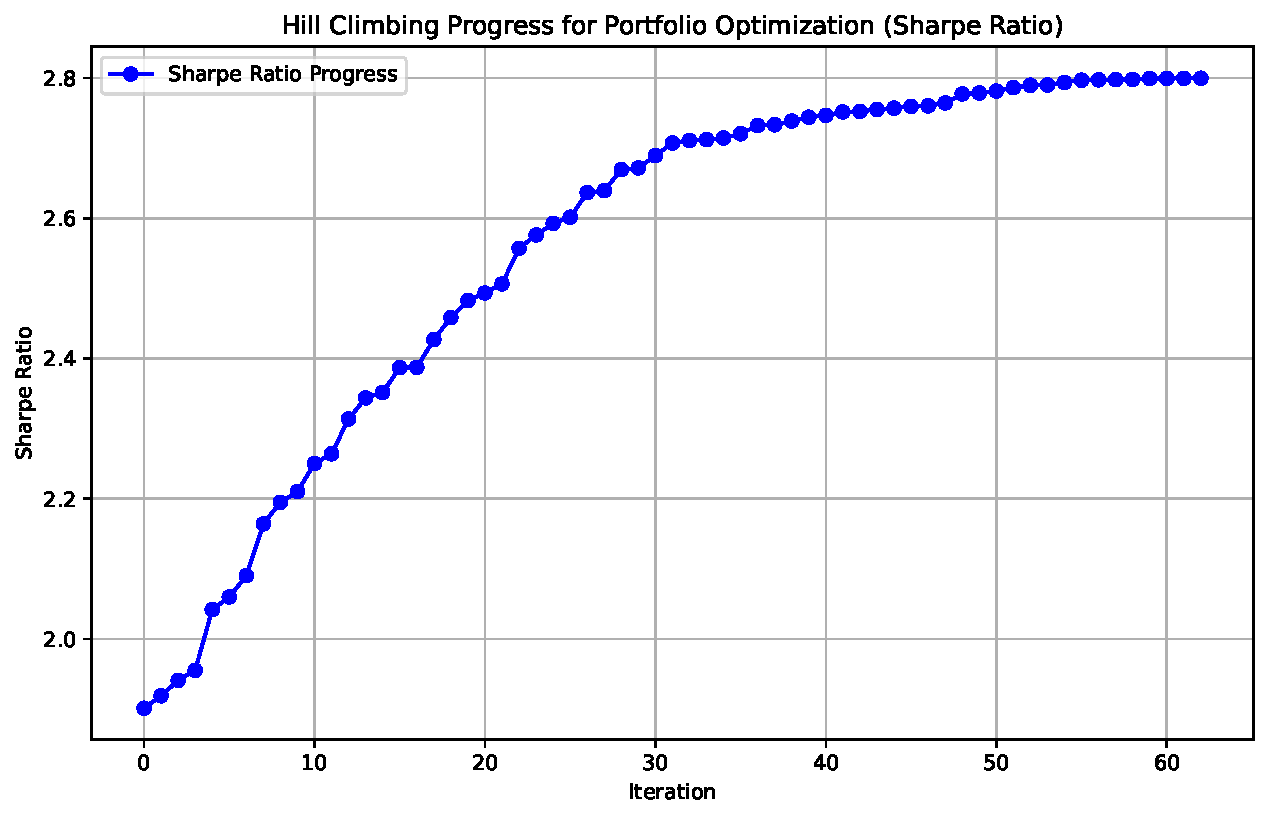
\includegraphics[keepaspectratio]{hc_files/figure-pdf/cell-25-output-1.pdf}}

\begin{verbatim}
Best portfolio weights: [0.20944997 0.         0.         0.11527445 0.         0.21091741
 0.         0.30274302 0.16161515 0.        ]
Best Sharpe ratio: 2.7994305119849985
Best portfolio returns: 0.6292559377057803, Best risk: 0.22477998114680559
Hill Climbing Finance Example Execution time: 0.082001 seconds
\end{verbatim}

\begin{itemize}
\tightlist
\item
  The plot visualizes how the Sharpe ratio evolves over the iterations.
  This helps understand the performance of the hill climbing algorithm.
\item
  The weights are heavily concentrated in a few stocks, particularly:

  \begin{itemize}
  \tightlist
  \item
    stocks = {[}`AAPL', `GOOGL', `MSFT', `AMZN', `TSLA', `NFLX', `NVDA',
    `META', `DIS', `BA'{]}
  \item
    19.560444 \% in stock 1: AAPL: Apple
  \item
    13.030724 \% in stock 4: AMZN: Amazon
  \item
    19.665558 \% in stock 6: NFLX: Netflix
  \item
    30.926036 \% in stock 8: META: Facebook
  \item
    16.817237 \% in stock 9: DIS: Walt Disney Co
  \end{itemize}
\item
  A Sharpe ratio of 2.800 is generally considered very good. A Sharpe
  ratio above 1 is usually considered acceptable, above 2 is very good,
  and above 3 is excellent, indicating that your portfolio offers a high
  return per unit of risk.
\item
  Our portfolio is highly concentrated in just 5 out of the 10 assets.
  The algorithm has effectively zeroed out the remaining assets, which
  can either be a good or bad thing depending on the actual data.

  \begin{itemize}
  \tightlist
  \item
    Pros: Concentration might mean that the algorithm has found a
    combination of assets that offer the best Sharpe ratio, meaning it
    is maximizing returns while minimizing risk.
  \item
    Cons: Concentrating in a few assets can increase the overall risk
    due to lack of diversification.
  \end{itemize}
\end{itemize}

\section{Items To Consider}\label{items-to-consider}

\begin{itemize}
\tightlist
\item
  A Sharpe ratio of 2.800 is very good, suggesting that the portfolio
  has a favorable balance of return vs.~risk. This ratio indicates that
  for each unit of risk, your portfolio earns more than two times the
  return.
\item
  Whether this Sharpe ratio is truly impressive depends on the quality
  and volatility of the returns in the dataset. Financial markets rarely
  produce consistently high Sharpe ratios, so the high value might
  indicate the presence of some anomaly, or it could be due to a limited
  timeframe or low volatility in the assets during this period.
\item
  Given the high concentration in a few stocks, there's a risk that the
  algorithm might be overfitting to the specific data in the training
  period. This means the portfolio might perform very well during the
  period used for the analysis but might not generalize well to future
  periods.
\item
  Things to Try Next:

  \begin{itemize}
  \tightlist
  \item
    Backtesting: Test this portfolio over a different time period or a
    longer time horizon to see if it maintains its high Sharpe ratio.
  \item
    Rebalancing: Consider rebalancing the portfolio periodically
    (monthly or quarterly) to see if the high Sharpe ratio persists.
  \item
    Diversification: If you are concerned about high concentration risk,
    you might want to introduce constraints to the hill climbing
    algorithm to enforce a minimum weight for diversification or limit
    the maximum weight of any asset.
  \end{itemize}
\end{itemize}

\bookmarksetup{startatroot}

\chapter{Using AI}\label{using-ai-5}

\begin{itemize}
\tightlist
\item
  Use the following prompt on a generative AI, like chatGPT, to learn
  more about the topics covered.
\item
  Hill Climbing Basics: Explain, in your own words, what hill climbing
  is and how it works as an optimization algorithm. How does it differ
  from exhaustive search?
\item
  Key Characteristics: Discuss the characteristics of hill climbing,
  such as its greedy approach and focus on local search. Why might these
  features cause hill climbing to get stuck in local optima?
\item
  Hill Climbing Steps: Implement the hill climbing algorithm for the
  OneMax problem using the pseudocode provided in the slides. How does
  the algorithm ensure progress toward an optimal solution?
\item
  Binary String Optimization: Modify the run\_hc function to allow the
  comparison operator \textgreater= instead of \textgreater. Analyze how
  this change affects the results when applied to a deceptive problem.
\item
  Challenges of Hill Climbing: Identify scenarios where hill climbing
  would fail to find the global optimum due to local maxima, plateaus,
  or ridges. Propose modifications to overcome these limitations.
\item
  Compare the results of hill climbing and exhaustive search for the
  same problem (e.g., OneMax). Under what conditions does hill climbing
  achieve similar results to exhaustive search?
\item
  Local vs Global Optima: Reflect on the importance of distinguishing
  between local and global optima in optimization problems. How can a
  better understanding of the solution landscape help in designing more
  effective algorithms?
\end{itemize}

\bookmarksetup{startatroot}

\chapter{Conlcusions}\label{conlcusions}

\begin{itemize}
\tightlist
\item
  In conclusion, the Hill Climbing algorithm provides a powerful yet
  straightforward approach for optimization by iteratively improving
  upon a solution within its local neighborhood. While its simplicity
  and efficiency make it suitable for various applications, it is
  inherently limited by its tendency to get stuck in local optima,
  especially in complex search landscapes with plateaus or ridges. The
  algorithm's effectiveness can be enhanced with variations like
  stochastic hill climbing or simulated annealing, which help in
  navigating these challenges. In applied scenarios, such as portfolio
  optimization, Hill Climbing can efficiently identify solutions that
  maximize objectives like the Sharpe ratio, though it may lead to
  highly concentrated solutions that require careful consideration
  regarding diversification and risk management.
\end{itemize}

\bookmarksetup{startatroot}

\chapter{Simulated Annealing}\label{simulated-annealing}

\bookmarksetup{startatroot}

\chapter{What is a Metaheuristic
Algorithm?}\label{what-is-a-metaheuristic-algorithm}

\begin{itemize}
\tightlist
\item
  One of the main attributes of a metaheuristic algorithm is that it
  performs a certain set of operators for a certain number of iterations
  to search for the optimal solution with great shrewdness.
\item
  Compared to the Exhaustive Search (ES) and hill climbing (HC)
  algorithms, a metaheuristic algorithm will neither check all the
  candidate solutions of a complex optimization problem like ES nor fall
  into a local optimum at early iterations as easily as HC.
\end{itemize}

\section{History of Metaheuristics}\label{history-of-metaheuristics}

\begin{itemize}
\tightlist
\item
  Although the term ``metaheuristic'' was introduced in the 1980s,
  several metaheuristic algorithms were actually presented in the 1960s
  or even earlier.
\item
  The year 1990 can be regarded as the first watershed in the
  development of metaheuristic algorithms. However, the available
  computing power may not satisfy the requirements of some complicated
  metaheuristic algorithms.
\item
  Since the late 1990s, the number of metaheuristic algorithms has
  exploded. More and more studies use ``the number of evaluations'' to
  replace ``the number of iterations'' for evaluating the performance of
  a metaheuristic algorithm because each search can be regarded as an
  investment of computation resource.

  \begin{itemize}
  \tightlist
  \item
    Using the number of evaluations provides a way that is more precise
    than using the number of iterations to evaluate the effect
    (improvement or outcome) of adding an additional unit of computation
    resource for the search
  \end{itemize}
\item
  From the year 2010 or even earlier, some groups have attempted to
  apply metaheuristic algorithms in high-performance computing
  environments.

  \begin{itemize}
  \tightlist
  \item
    Using distributed or parallel computing systems to accelerate the
    response time of metaheuristic algorithms is an intuitive approach
    adopted in some early studies.
  \item
    Some of the parallel metaheuristics are not only able to provide the
    end results to the user more quickly; they also can find better
    results than metaheuristic algorithms on a single machine because
    the parallel computing mechanism leads them to increase the search
    diversity during the convergence process.
  \item
    When we look at these distributed and parallel computing
    environments, the cloud computing platform (e.g., Hadoop, Spark,
    Microsoft Azure, Amazon EC2, or Google Compute Engine) can now
    provide an easy way to use a distributed computing system to further
    reduce the response time of metaheuristics.
  \end{itemize}
\end{itemize}

\section{A Unified Framework for Metaheuristic Algorithms
(UFM)}\label{a-unified-framework-for-metaheuristic-algorithms-ufm}

\begin{itemize}
\tightlist
\item
  The appearance of metaheuristic algorithms has come with methods to
  classify them. These classification methods include:
\end{itemize}

\begin{enumerate}
\def\labelenumi{(\arabic{enumi})}
\tightlist
\item
  nature-inspired vs.~non-nature inspired,
\item
  dynamic vs.~static objective function,
\item
  one vs.~various neighborhood structures,
\item
  memory usage vs.~memoryless methods,
\item
  with vs.~without local search method, and
\item
  population-based vs.~single-solution-based search.
\end{enumerate}

\section{UFM 5 Main Operators}\label{ufm-5-main-operators}

\begin{enumerate}
\def\labelenumi{\arabic{enumi}.}
\tightlist
\item
  Initialization (I): The initialization operator normally plays the
  roles of reading the input file (e.g., dataset), initializing all the
  parameters of a metaheuristic algorithm, and determining the initial
  solutions, which is normally based on a random process.
\item
  Transition (T): The transition operator usually plays the role of
  varying the search directions, such as perturbing a portion of the
  subsolutions of the current solution to generate a new candidate
  solution or generating a set of new candidate solutions each based on
  two or more of the current solutions.
\item
  Evaluation (E): The evaluation operator is responsible for measuring
  the quality of solutions, such as calculating the objective value of
  each solution to be used by the determination operator to distinguish
  the quality of all the solutions. An intuitive way is to use an
  objective function to measure the quality of a solution for the
  problem in question. However, some metaheuristics do not use the
  ``objective value'' directly to measure their solutions; rather, the
  objective value of a solution has to undergo some sort of
  transformation to obtain the so-called ``fitness value.''
\item
  Determination (D): The determination operator plays the role of
  deciding the search directions by using information the evaluation
  operator provides during the convergence process. The performance of a
  metaheuristic algorithm depends to a large extent on the performance
  of this operator. A ``good'' search strategy for this operator will
  make it possible for the metaheuristic algorithm to find a better
  solution faster or to avoid falling into a local optimum at early
  iterations.
\item
  Output (O): In spite of the fact that this operator seems to be
  trivial, the reality is that it can be either simple or complex
  depending on how much information we want to display for the
  metaheuristic algorithm. It can be as simple as displaying only the
  final result of the metaheuristic algorithm, or it can be as complex
  as displaying the trajectory of convergence of the metaheuristic
  algorithm to better understand the performance of a metaheuristic
  algorithm.
\end{enumerate}

\section{UFM}\label{ufm}

\begin{itemize}
\tightlist
\item
  In this framework, I denotes the input dataset, s denotes the current
  solution, \(\nu\) denotes the candidate solution, \(f_s\) denotes the
  objective value of \(s\), and \(f_\nu\) denotes the objective value of
  \(\nu\). Also, \(s\) and \(\nu\) can denote either a single solution
  or a set of solutions, where each solution has \(n\) elements or is an
  \(n-tuple\).
\end{itemize}

\begin{figure}[H]

{\centering \pandocbounded{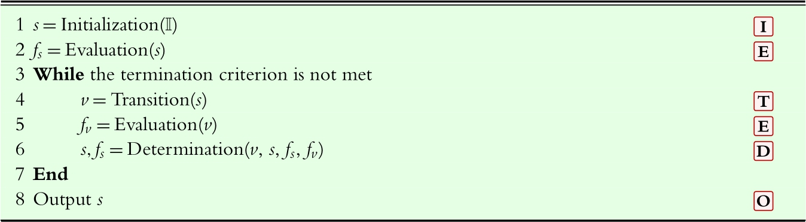
\includegraphics[keepaspectratio]{Pictures/UFM.png}}

}

\caption{UFM}

\end{figure}%

\section{Comparison between exhaustive search, greedy, and metaheuristic
algorithms}\label{comparison-between-exhaustive-search-greedy-and-metaheuristic-algorithms}

\begin{figure}[H]

{\centering \pandocbounded{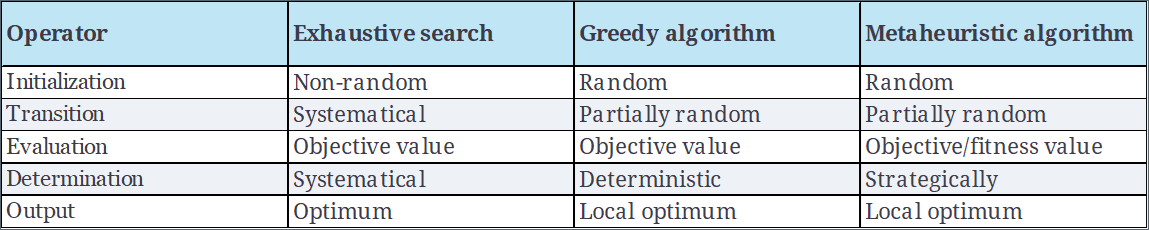
\includegraphics[keepaspectratio]{Pictures/compare.png}}

}

\caption{Compare Models}

\end{figure}%

\bookmarksetup{startatroot}

\chapter{Simulated Annealing (SA)}\label{simulated-annealing-sa}

\begin{itemize}
\item
  If life is like simulated annealing, what's the most memorable
  `temperature drop' moment where you had to settle down and stick to
  one choice?
\item
  A single-solution-based algorithm
\item
  A probabilistic optimization algorithm inspired by the annealing
  process in metallurgy, where materials are heated and then slowly
  cooled to reduce defects, thereby optimizing their structural
  properties.
\item
  In optimization, SA is used to find a good approximation to the global
  minimum of a function in a large search space, particularly when the
  search space is discrete or contains multiple local minima.
\item
  The search strategy of SA is to start with a random possible solution
  in the solution space and then use the Metropolis acceptance criterion
  to determine whether a worse solution is to be accepted or not.
\item
  To emulate the annealing process for a minimization optimization
  problem, SA will first calculate the difference between the objective
  values of the new candidate solution \(\nu\) and the current solution
  \(s\) to see whether it will accept the new candidate solution or not,
  as follows: \(\Delta_f^{\text{min}} = f(\nu) - f(s)\)
\end{itemize}

\section{Key Components}\label{key-components}

\begin{itemize}
\tightlist
\item
  Solution Space:

  \begin{itemize}
  \tightlist
  \item
    This is the space of all possible solutions to the problem.
  \end{itemize}
\item
  Objective Function:

  \begin{itemize}
  \tightlist
  \item
    Defines the quality of a solution (usually the cost or energy to
    minimize).
  \item
    For instance, in the Travelling Salesman Problem (TSP), the
    objective function would be the total distance of the tour.
  \end{itemize}
\item
  Temperature:

  \begin{itemize}
  \tightlist
  \item
    This controls the probability of accepting worse solutions.
  \item
    Initially, the temperature is high, allowing the algorithm to
    explore the solution space more freely.
  \item
    As the temperature lowers, the algorithm becomes more conservative,
    accepting only smaller degradations in the objective.
  \end{itemize}
\item
  Cooling Schedule:

  \begin{itemize}
  \tightlist
  \item
    This is a function that dictates how the temperature decreases over
    time (iterations).
  \item
    Typically, it follows a geometric decay, where the temperature
    decreases by a factor on each iteration (e.g.,
    \(T = T_0 * \alpha^k\), where \(T_0\) is the initial temperature,
    alpha is a constant, and \(k\) is the iteration number).
  \end{itemize}
\end{itemize}

\section{Defining SA}\label{defining-sa}

\begin{itemize}
\tightlist
\item
  An iterative algorithm that explores the solution space of an
  optimization problem by considering not only improvements to the
  current solution but also occasional, controlled acceptance of worse
  solutions. This allows the algorithm to escape local minima and
  explore a broader range of the search space in search of a global
  minimum.

  \begin{itemize}
  \tightlist
  \item
    The function \(f(x)\) that the algorithm seeks to minimize (or
    maximize)
  \item
    The configuration or state is a point \(x\) in the solution space,
    representing a possible solution to the problem.
  \item
    The neighboring states are the set of solutions that are reachable
    from the current state through small modifications.
  \item
    A control parameter temperature \(T\)) that regulates the likelihood
    of accepting worse solutions. It starts high and gradually decreases
    as the algorithm progresses.
  \item
    As \(T\) decreases, the probability of accepting worse solutions
    decreases, making the search more focused on local improvements.
  \item
    A cooling schedule includes a function that controls the decrease of
    the temperature T over time
  \end{itemize}
\end{itemize}

\section{Usefulness of SA}\label{usefulness-of-sa}

\begin{itemize}
\tightlist
\item
  The basic idea of SA is to occasionally accept non-improving
  solutions, which means that SA will not always move to a better
  solution.
\item
  Simulated Annealing is widely used in various fields, such as:

  \begin{itemize}
  \tightlist
  \item
    Combinatorial Optimization: Problems like the Traveling Salesman
    Problem (TSP), scheduling, and circuit design.
  \item
    Machine Learning: Hyperparameter optimization, clustering.
  \item
    Engineering: Structural design, control systems.
  \end{itemize}
\item
  Practical Applications: real-world problems where SA shines: vehicle
  routing, job scheduling, or portfolio optimization.
\end{itemize}

\section{Tuning Parameters}\label{tuning-parameters}

\begin{itemize}
\tightlist
\item
  The success of SA heavily depends on the tuning of parameters like the
  cooling schedule, the initial temperature, and the size of the
  neighborhood.

  \begin{itemize}
  \tightlist
  \item
    hyperparameter tuning and experimentation.
  \end{itemize}
\item
  Comparison to Other Algorithms: To compare SA to algorithms like
  Genetic Algorithms (GA) or Greedy Heuristics, SA is more appropriate
  due to its exploration-exploitation trade-off. Where
  \textbf{exploration} (searching the solution space broadly) and
  \textbf{exploitation} (focusing on refining the best solutions found
  so far).
\end{itemize}

\section{The Search Strategy of SA}\label{the-search-strategy-of-sa}

\begin{itemize}
\tightlist
\item
  Start with a random possible solution in the solution space and then
  use the Metropolis acceptance criterion to determine whether a worse
  solution is to be accepted or not.
\item
  In this example, \(t^{\Delta} \quad\) and \(\quad t^{\nabla}\)
  indicate that the solution at the \(t+1^{\text{th}}\) iteration is
  either better or not better than the solution at the \(t^{\text{th}}\)
  iteration, respectively.
\item
  This example shows that if the starting point is 𝑥\_9 and SA accepts
  only a new candidate solution that is better than the current
  solution, i.e., it has no escape mechanism, the search will get stuck
  at one of the two local optima (\(x_8\) and \(x_10\)) denoted \(L_1\)
  and \(L_2\).
\end{itemize}

\begin{figure}[H]

{\centering \pandocbounded{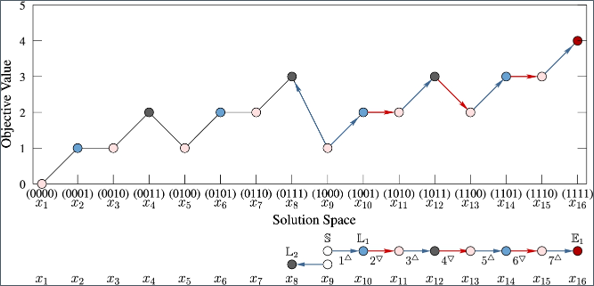
\includegraphics[keepaspectratio]{Pictures/sa.png}}

}

\caption{Search Strategy of SA}

\end{figure}%

\section{SA Algorithm}\label{sa-algorithm}

\begin{itemize}
\tightlist
\item
  Initialization:

  \begin{itemize}
  \tightlist
  \item
    Choose an initial solution \(x_0\) and an initial temperature
    \(T_0\).
  \end{itemize}
\item
  Iteration:

  \begin{itemize}
  \tightlist
  \item
    For each step, generate a neighboring solution \(x^′\) of the
    current solution \(x\).
  \item
    Compute the change in the objective function.
  \item
    Decide whether to move to the new solution \(x^′\) based on the
    acceptance probability.
  \item
    Gradually reduce the temperature \(T\) according to the cooling
    schedule
  \end{itemize}
\item
  Termination:

  \begin{itemize}
  \tightlist
  \item
    The algorithm stops when the temperature \(T\) is sufficiently low
    or after a predefined number of iterations.
  \item
    The best solution found during the process is returned.
  \end{itemize}
\end{itemize}

\begin{figure}[H]

{\centering \pandocbounded{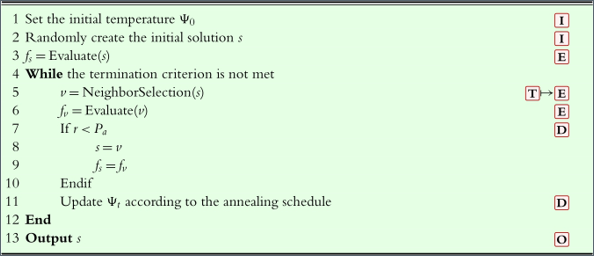
\includegraphics[keepaspectratio]{Pictures/sa1.png}}

}

\caption{SA Algorithm}

\end{figure}%

\section{Many Versions of SA Exist}\label{many-versions-of-sa-exist}

\begin{itemize}
\tightlist
\item
  This framework is a little bit different from the model above because
  there are two loops (outer and inner loops). This implies that a
  certain number of new candidate solutions will be generated and
  evaluated before the temperature is updated.
\end{itemize}

\begin{figure}[H]

{\centering \pandocbounded{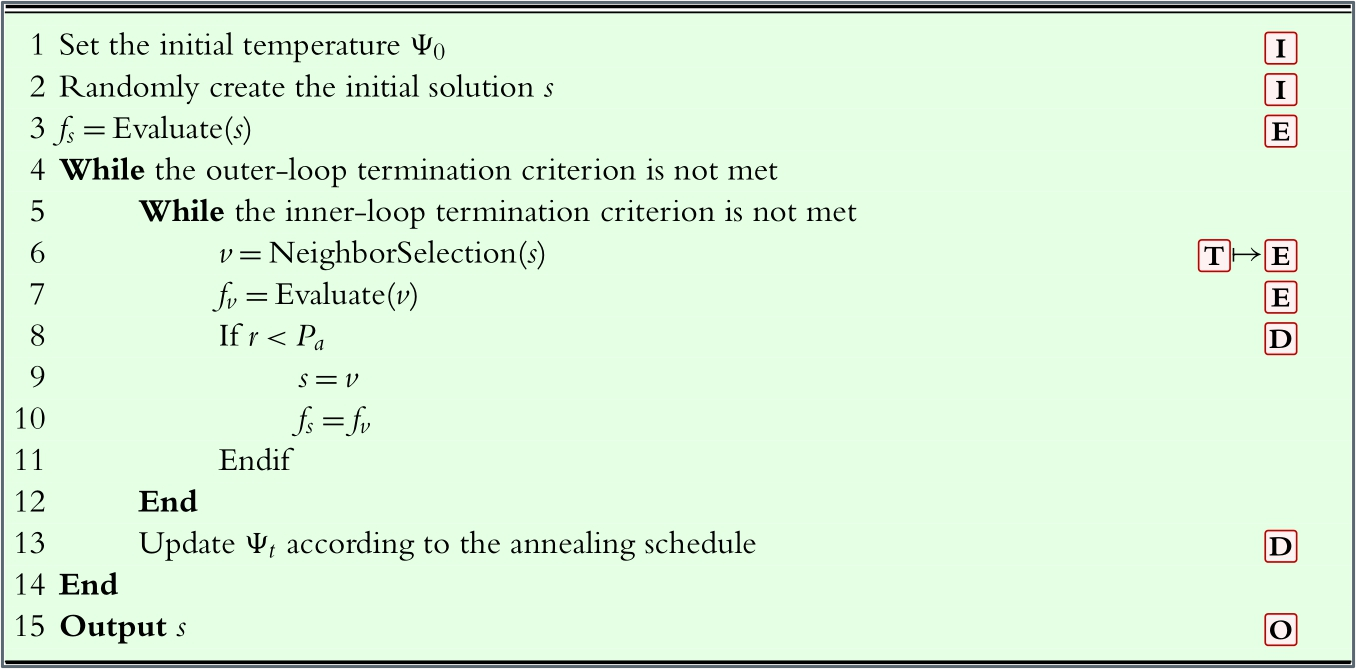
\includegraphics[keepaspectratio]{Pictures/sa2.png}}

}

\caption{SA Algorithm Variation}

\end{figure}%

\section{Advantages and Disadvantages of
SA}\label{advantages-and-disadvantages-of-sa}

\subsection{Advantages}\label{advantages}

\begin{itemize}
\tightlist
\item
  Global Search Capability: Unlike simple greedy algorithms, simulated
  annealing can escape local minima and potentially find a global
  minimum.
\item
  Flexibility: It can be applied to a wide range of optimization
  problems, including those with complex, multimodal landscapes.
\item
  Simplicity: The algorithm is relatively easy to implement and does not
  require gradient information, making it suitable for
  non-differentiable problems.
\end{itemize}

\subsection{Disadvantages}\label{disadvantages}

\begin{itemize}
\tightlist
\item
  Computational Cost: The method can be slow, particularly for large
  problem spaces, as it requires many iterations to reach a good
  solution.
\item
  Parameter Sensitivity: The performance of simulated annealing depends
  heavily on the choice of the cooling schedule, initial temperature,
  and other parameters.
\item
  No Guarantee of Optimality: The algorithm does not guarantee finding
  the global optimum but rather a good approximation.
\end{itemize}

\bookmarksetup{startatroot}

\chapter{SA Algorithm}\label{sa-algorithm-1}

\begin{itemize}
\item
  To emulate the annealing process for a minimization optimization
  problem, SA will first calculate the difference between the objective
  values of the new candidate solution v and the current solution s to
  see whether it will accept the new candidate solution or not.
  \[\Delta_f^{\text{min}} = f(\nu) - f(s)\]
\item
  In case the difference between the objective values is less than
  \(0\), SA will accept the new candidate solution as the current
  solution, which means that \(\nu\) replaces; otherwise, SA will
  calculate a probability to decide whether or not to accept a
  non-improving candidate solution.
\item
  \(p_a^{\text{min}} = \exp \left( \frac{-(f(v) - f(s))}{\Psi_t} \right) = \exp \left( \frac{f(s) - f(v)}{\Psi_t} \right),\)
  where where \(f(x)\) denotes the evaluation function, s denotes the
  current solution, \(\nu\) denotes the new solution, and \(\Psi_t\)
  denotes the temperature at the \(t\)-th iteration.
\item
  To apply SA to a maximization optimization problem, all we have to do
  is to negate the difference with the following:
  \[\Delta_f^{\text{max}} -\Delta_f^{\text{min}} = -f(v) - -f(s) = f(s)-f(v)\]
\item
  Such a modification makes it possible to check
  \(\Delta_f^{\text{max}}\) in a similar way; that
  is,\(\Delta_f^{\text{max}}<0\), SA will accept the new candidate
  solution as the current solution; otherwise, SA will again calculate a
  probability to decide whether or not to accept a non-improving
  candidate solution for the following:
  \[p_a^{\text{max}} = \exp \left( \frac{-(f(s) - f(v))}{\Psi_t} \right) = \exp \left( \frac{f(v) - f(s)}{\Psi_t} \right)\].
\end{itemize}

\section{Examples of How Value Can
Change}\label{examples-of-how-value-can-change}

\begin{figure}[H]

{\centering \pandocbounded{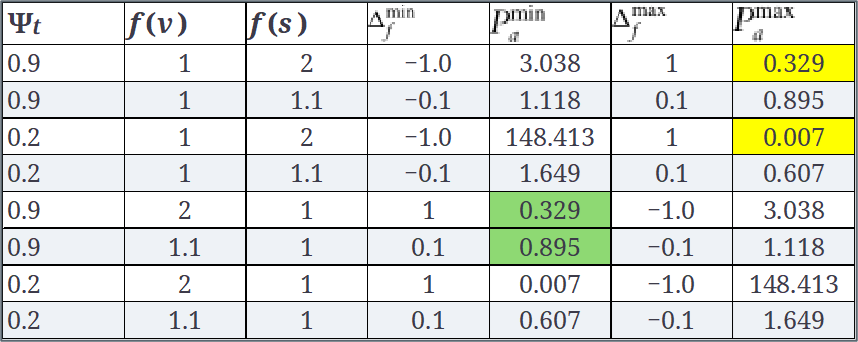
\includegraphics[keepaspectratio]{Pictures/sa3.png}}

}

\caption{SA Changing Values}

\end{figure}%

\begin{itemize}
\tightlist
\item
  In this case, \(p_a^{\text{max}}\)=.329 and 0.007 for \({\Psi_t}\) =
  .9 and 0.2, respectively. This indicates that a lower temperature
  Image implies a smaller probability Image to accept a non-improving
  candidate solution as the current solution.
\item
  The value of \(f_s\) goes from 2.0 to 1.1, the value of
  \(p_a^{\text{max}}\) goes from 0.329 up to 0.895. This means that in
  case \(f(\nu\)\$ is worse than \(f(s)\), a smaller
  \(\Delta_f^{\text{max}}\) implies a higher probability
  \(p_a^{\text{max}}\) to accept a non-improving candidate solution as
  the current solution.
\end{itemize}

\subsection{Summary of Cases}\label{summary-of-cases}

\begin{itemize}
\tightlist
\item
  The new solution v is better than the current solution s.

  \begin{itemize}
  \tightlist
  \item
    SA will always accept the new solution owing to the fact that
    \(P_A\) will always be greater than 1.0 and \(r \in [0,1]\) will
    always be smaller than \(P_A\). The new solution \(\nu\) is worse
    than the current solution \(s\). SA will accept the new solution
    only if \(r < P_A\) , where \(r\) is as defined above. The new
    solution \(\nu\) is worse than the current solution s. SA will not
    accept the new solution because \(r \geq P_A\) .
  \end{itemize}
\end{itemize}

\section{Comparing Algorithms}\label{comparing-algorithms}

\begin{itemize}
\tightlist
\item
  Simulated Annealing Algorithms

  \begin{itemize}
  \tightlist
  \item
    Exploration: In the early stages, SA accepts worse solutions with
    high probability, which allows it to explore the search space more
    broadly and escape local optima.
  \item
    Exploitation: As the temperature decreases, the algorithm becomes
    more conservative and starts focusing on refining the current
    solution. SA balances exploration and exploitation dynamically as
    the temperature cools.
  \item
    Trade-off: SA is particularly good when the solution space is rugged
    (many local optima) because it has a built-in mechanism
    (temperature) to transition from exploration to exploitation.
  \end{itemize}
\item
  Genetic Algorithms

  \begin{itemize}
  \tightlist
  \item
    Exploration: GA uses processes like mutation and crossover to
    generate new solutions from the current population. Mutation allows
    for exploration by introducing random changes, while crossover
    exploits good solutions by combining them.
  \item
    Exploitation: GA exploits the best solutions through selection and
    crossover, where solutions with higher fitness are more likely to
    survive and reproduce.
  \item
    Trade-off: GA maintains a population of solutions, which helps with
    exploration, but can sometimes suffer from premature convergence if
    the population becomes too homogeneous, leading to poor exploitation
    of potentially better solutions.
  \end{itemize}
\item
  Greedy Algorithms

  \begin{itemize}
  \tightlist
  \item
    Exploration: Greedy algorithms have very limited exploration. They
    make the best immediate choice (locally optimal) at each step
    without considering the broader solution space.
  \item
    Exploitation: Greedy heuristics are purely exploitative---they focus
    solely on improving the current state as much as possible. They tend
    to get stuck in local optima because they don't explore alternative
    solutions that might initially look worse but could lead to better
    outcomes.
  \item
    Trade-off: A greedy algorithm doesn't balance exploration and
    exploitation well. It is fast and simple but can fail when the
    problem has many local optima, making it inappropriate for complex
    problems like TSP or scheduling.
  \end{itemize}
\end{itemize}

\subsection{When SA Is More
Appropriate}\label{when-sa-is-more-appropriate}

\begin{itemize}
\tightlist
\item
  Rugged Solution Spaces: When there are many local optima (like in the
  Travelling Salesman Problem or complex scheduling), SA's ability to
  accept worse solutions helps it explore more and avoid local traps.
\item
  Time-Constrained Search: SA can be more useful when you don't need an
  exact global optimum but want a good solution within a reasonable
  amount of time. The cooling schedule can be adjusted to control how
  fast the algorithm converges.
\end{itemize}

\bookmarksetup{startatroot}

\chapter{Making a Model: One Max with
SA}\label{making-a-model-one-max-with-sa}

\section{Imports, Global Variables}\label{imports-global-variables}

\begin{Shaded}
\begin{Highlighting}[]
\CommentTok{\#\#Simulated Annealing One{-}Max Example}
\ImportTok{import}\NormalTok{ numpy }\ImportTok{as}\NormalTok{ np}
\ImportTok{import}\NormalTok{ random}
\ImportTok{import}\NormalTok{ matplotlib.pyplot }\ImportTok{as}\NormalTok{ plt}
\ImportTok{import}\NormalTok{ time}

\CommentTok{\# Define the necessary global variables}
\NormalTok{num\_bits }\OperatorTok{=} \DecValTok{10}
\NormalTok{max\_iterations }\OperatorTok{=} \DecValTok{1000}
\NormalTok{initial\_temp }\OperatorTok{=} \DecValTok{10}
\NormalTok{cooling\_rate }\OperatorTok{=} \FloatTok{0.99}
\NormalTok{min\_temp }\OperatorTok{=} \FloatTok{0.0001}
\end{Highlighting}
\end{Shaded}

\section{Initialize}\label{initialize}

\begin{itemize}
\tightlist
\item
  The init\_sa function initializes a random solution (sol) for the
  One-Max problem by generating a binary array of size num\_bits
  (default 10), where each element is randomly set to 0 or 1.The initial
  solution is evaluated using the One-Max function (evaluate) to
  calculate its fitness (i.e., the sum of 1's in the array).The function
  returns the initial solution and its evaluated fitness.
\end{itemize}

\begin{Shaded}
\begin{Highlighting}[]
\CommentTok{\# Initialization function (I)}
\KeywordTok{def}\NormalTok{ init\_sa(num\_bits):}
\NormalTok{    sol }\OperatorTok{=}\NormalTok{ np.random.randint(}\DecValTok{0}\NormalTok{, }\DecValTok{2}\NormalTok{, num\_bits)}
    \ControlFlowTok{return}\NormalTok{ sol, evaluate(sol)}
\end{Highlighting}
\end{Shaded}

\subsection{Transition (T)}\label{transition-t}

\begin{itemize}
\tightlist
\item
  The transit function generates a neighboring solution by flipping a
  random bit in the current solution.
\item
  This is done by randomly selecting an index in the binary array and
  toggling the bit (changing 1 to 0 or 0 to 1).
\item
  This new solution represents the neighboring candidate that will be
  evaluated next, which is a small random change to the current
  solution.
\end{itemize}

\begin{Shaded}
\begin{Highlighting}[]
\CommentTok{\# Transition function (T)}
\KeywordTok{def}\NormalTok{ transit(sol):}
\NormalTok{    new\_sol }\OperatorTok{=}\NormalTok{ sol.copy()}
\NormalTok{    index }\OperatorTok{=}\NormalTok{ np.random.randint(}\BuiltInTok{len}\NormalTok{(sol))}
\NormalTok{    new\_sol[index] }\OperatorTok{=} \DecValTok{1} \OperatorTok{{-}}\NormalTok{ new\_sol[index]  }\CommentTok{\# Flip a random bit}
    \ControlFlowTok{return}\NormalTok{ new\_sol}
\end{Highlighting}
\end{Shaded}

\subsection{Evaluate (E)}\label{evaluate-e}

\begin{itemize}
\tightlist
\item
  The evaluate function calculates the fitness of the current solution
  by summing up the number of 1's in the binary array (sol).The One-Max
  problem aims to maximize this value, with the goal being to find the
  solution with all bits set to 1.
\end{itemize}

\begin{Shaded}
\begin{Highlighting}[]
\CommentTok{\# Evaluation Function (E): One{-}max function}
\KeywordTok{def}\NormalTok{ evaluate(sol):}
    \ControlFlowTok{return}\NormalTok{ np.}\BuiltInTok{sum}\NormalTok{(sol)}
\end{Highlighting}
\end{Shaded}

\subsection{Determination (D)}\label{determination-d}

\begin{itemize}
\tightlist
\item
  The determine function decides whether to accept the new neighboring
  solution (neighbor\_value), based on its value compared to the current
  solution (current\_value).
\item
  If the neighboring solution is better (i.e., it has a higher One-Max
  value), it is accepted.
\item
  If the neighboring solution is worse, it may still be accepted based
  on the probability calculated by the simulated annealing algorithm:

  \begin{itemize}
  \tightlist
  \item
    The acceptance probability depends on the temperature and the
    difference between the new and current values.
  \item
    A higher temperature allows for more exploration of worse solutions,
    while a lower temperature makes the algorithm more selective.
  \end{itemize}
\item
  The function returns True if the new solution is accepted, otherwise
  False.
\end{itemize}

\begin{Shaded}
\begin{Highlighting}[]
\CommentTok{\# Determination function for SA (D)}
\KeywordTok{def}\NormalTok{ determine(neighbor\_value, current\_value, temperature):}
    \ControlFlowTok{if}\NormalTok{ neighbor\_value }\OperatorTok{\textgreater{}}\NormalTok{ current\_value:}
        \ControlFlowTok{return} \VariableTok{True}
    \ControlFlowTok{else}\NormalTok{:}
\NormalTok{        acceptance\_probability }\OperatorTok{=}\NormalTok{ np.exp((neighbor\_value }\OperatorTok{{-}}\NormalTok{ current\_value) }\OperatorTok{/}\NormalTok{ temperature)}
        \ControlFlowTok{return}\NormalTok{ random.random() }\OperatorTok{\textless{}}\NormalTok{ acceptance\_probability}
\end{Highlighting}
\end{Shaded}

\subsection{Run Function}\label{run-function}

\begin{itemize}
\tightlist
\item
  The init\_sa function generates a random initial solution
  (current\_sol) with a binary array of length num\_bits.
\item
  This solution is evaluated using the evaluate function, which counts
  the number of 1's in the array.
\item
  The current solution is also set as the best solution initially, since
  no other solutions have been explored yet.
\item
  The temperature is set to initial\_temp (default 10), which controls
  the probability of accepting worse solutions in the early stages of
  the algorithm.
\item
  The list value\_history is initialized to store the value (fitness) of
  the current solution over time.
\item
  This main loop runs until the temperature drops below min\_temp
  (0.0001) or the maximum number of iterations (max\_iterations, default
  1000) is reached. Each iteration represents one step in the simulated
  annealing process.
\item
  A neighboring solution (neighbor\_sol) is generated by the transit
  function, which randomly flips one bit in the current solution. * This
  represents exploring a new area of the search space close to the
  current solution.
\item
  The neighboring solution is evaluated using the evaluate function,
  which calculates its fitness (i.e., the number of 1's in the binary
  array). This value is compared to the current solution's fitness.
\item
  The determine function decides whether to accept the neighboring
  solution
\item
  The current solution's fitness is appended to value\_history to keep a
  record of the solution's fitness across iterations. This will later be
  used to plot the progress of the algorithm.
\item
  After each iteration, the temperature is reduced by multiplying it by
  the cooling\_rate (default 0.99). This cooling process gradually
  reduces the probability of accepting worse solutions, making the
  algorithm behave more like greedy hill climbing toward the end.
\item
  The number of iterations is incremented.
\item
  After the loop terminates (either because the temperature has cooled
  sufficiently or the maximum number of iterations has been reached),
  the function returns:best\_sol: The best solution found during the
  process.best\_value: The fitness value of the best
  solution.value\_history: A list of the fitness values over time,
  useful for visualizing the algorithm's progress.
\end{itemize}

\begin{Shaded}
\begin{Highlighting}[]
\CommentTok{\# Simulated Annealing (SA) function}
\KeywordTok{def}\NormalTok{ simulated\_annealing(num\_bits):}
\NormalTok{    current\_sol, current\_value }\OperatorTok{=}\NormalTok{ init\_sa(num\_bits)}
\NormalTok{    best\_sol, best\_value }\OperatorTok{=}\NormalTok{ current\_sol, current\_value}
\NormalTok{    temperature }\OperatorTok{=}\NormalTok{ initial\_temp}
\NormalTok{    value\_history }\OperatorTok{=}\NormalTok{ [current\_value]}

\NormalTok{    iterations }\OperatorTok{=} \DecValTok{0}
    \ControlFlowTok{while}\NormalTok{ temperature }\OperatorTok{\textgreater{}}\NormalTok{ min\_temp }\KeywordTok{and}\NormalTok{ iterations }\OperatorTok{\textless{}}\NormalTok{ max\_iterations:}
\NormalTok{        neighbor\_sol }\OperatorTok{=}\NormalTok{ transit(current\_sol)}
\NormalTok{        neighbor\_value }\OperatorTok{=}\NormalTok{ evaluate(neighbor\_sol)}

        \ControlFlowTok{if}\NormalTok{ determine(neighbor\_value, current\_value, temperature):}
\NormalTok{            current\_sol, current\_value }\OperatorTok{=}\NormalTok{ neighbor\_sol, neighbor\_value}
            \ControlFlowTok{if}\NormalTok{ current\_value }\OperatorTok{\textgreater{}}\NormalTok{ best\_value:}
\NormalTok{                best\_sol, best\_value }\OperatorTok{=}\NormalTok{ current\_sol, current\_value}

        \CommentTok{\# Store history of values for plotting}
\NormalTok{        value\_history.append(current\_value)}

        \CommentTok{\# Cool down the temperature}
\NormalTok{        temperature }\OperatorTok{*=}\NormalTok{ cooling\_rate}
\NormalTok{        iterations }\OperatorTok{+=} \DecValTok{1}

    \ControlFlowTok{return}\NormalTok{ best\_sol, best\_value, value\_history}
\end{Highlighting}
\end{Shaded}

\subsection{Main Execution}\label{main-execution-3}

\begin{itemize}
\tightlist
\item
  The process starts by initializing the solution using Initialization
  (I) (init\_sa), followed by repeated transitions (T) and evaluations
  (E) to explore the search space.
\item
  After each transition, the Determination (D) function decides whether
  to accept the new solution based on the current temperature and
  fitness values.
\item
  The temperature gradually cools down, reducing the chance of accepting
  worse solutions as the algorithm progresses.
\item
  Finally, the results are printed and plotted for visual analysis.
\end{itemize}

\begin{Shaded}
\begin{Highlighting}[]
\CommentTok{\# Main execution}
\NormalTok{start\_time }\OperatorTok{=}\NormalTok{ time.time()}
\NormalTok{best\_sol, best\_value, value\_history }\OperatorTok{=}\NormalTok{ simulated\_annealing(num\_bits)}
\NormalTok{end\_time }\OperatorTok{=}\NormalTok{ time.time()}
\NormalTok{execution\_time }\OperatorTok{=}\NormalTok{ end\_time }\OperatorTok{{-}}\NormalTok{ start\_time}
\end{Highlighting}
\end{Shaded}

\section{Output}\label{output-3}

\begin{Shaded}
\begin{Highlighting}[]
\CommentTok{\# Output results (O)}
\BuiltInTok{print}\NormalTok{(}\SpecialStringTok{f"Best solution: }\SpecialCharTok{\{}\NormalTok{best\_sol}\SpecialCharTok{\}}\SpecialStringTok{"}\NormalTok{)}
\BuiltInTok{print}\NormalTok{(}\SpecialStringTok{f"Best value (number of 1s): }\SpecialCharTok{\{}\NormalTok{best\_value}\SpecialCharTok{\}}\SpecialStringTok{"}\NormalTok{)}
\BuiltInTok{print}\NormalTok{(}\SpecialStringTok{f"Execution time: }\SpecialCharTok{\{}\NormalTok{execution\_time}\SpecialCharTok{:.6f\}}\SpecialStringTok{ seconds"}\NormalTok{)}

\CommentTok{\# Plot the simulated annealing progress}
\NormalTok{plt.figure(figsize}\OperatorTok{=}\NormalTok{(}\DecValTok{10}\NormalTok{, }\DecValTok{6}\NormalTok{))}
\NormalTok{plt.plot(value\_history, marker}\OperatorTok{=}\StringTok{\textquotesingle{}o\textquotesingle{}}\NormalTok{, linestyle}\OperatorTok{=}\StringTok{\textquotesingle{}{-}{-}\textquotesingle{}}\NormalTok{, color}\OperatorTok{=}\StringTok{\textquotesingle{}blue\textquotesingle{}}\NormalTok{, label}\OperatorTok{=}\StringTok{\textquotesingle{}SA Progress\textquotesingle{}}\NormalTok{)}
\NormalTok{plt.title(}\StringTok{"One{-}Max Problem with Simulated Annealing Progress"}\NormalTok{)}
\NormalTok{plt.xlabel(}\StringTok{"Iteration"}\NormalTok{)}
\NormalTok{plt.ylabel(}\StringTok{"Objective Value (Number of 1s)"}\NormalTok{)}
\NormalTok{plt.legend()}
\NormalTok{plt.grid(}\VariableTok{True}\NormalTok{)}
\NormalTok{plt.show()}
\end{Highlighting}
\end{Shaded}

\begin{verbatim}
Best solution: [1 1 1 1 1 1 1 1 1 1]
Best value (number of 1s): 10
Execution time: 0.009000 seconds
\end{verbatim}

\pandocbounded{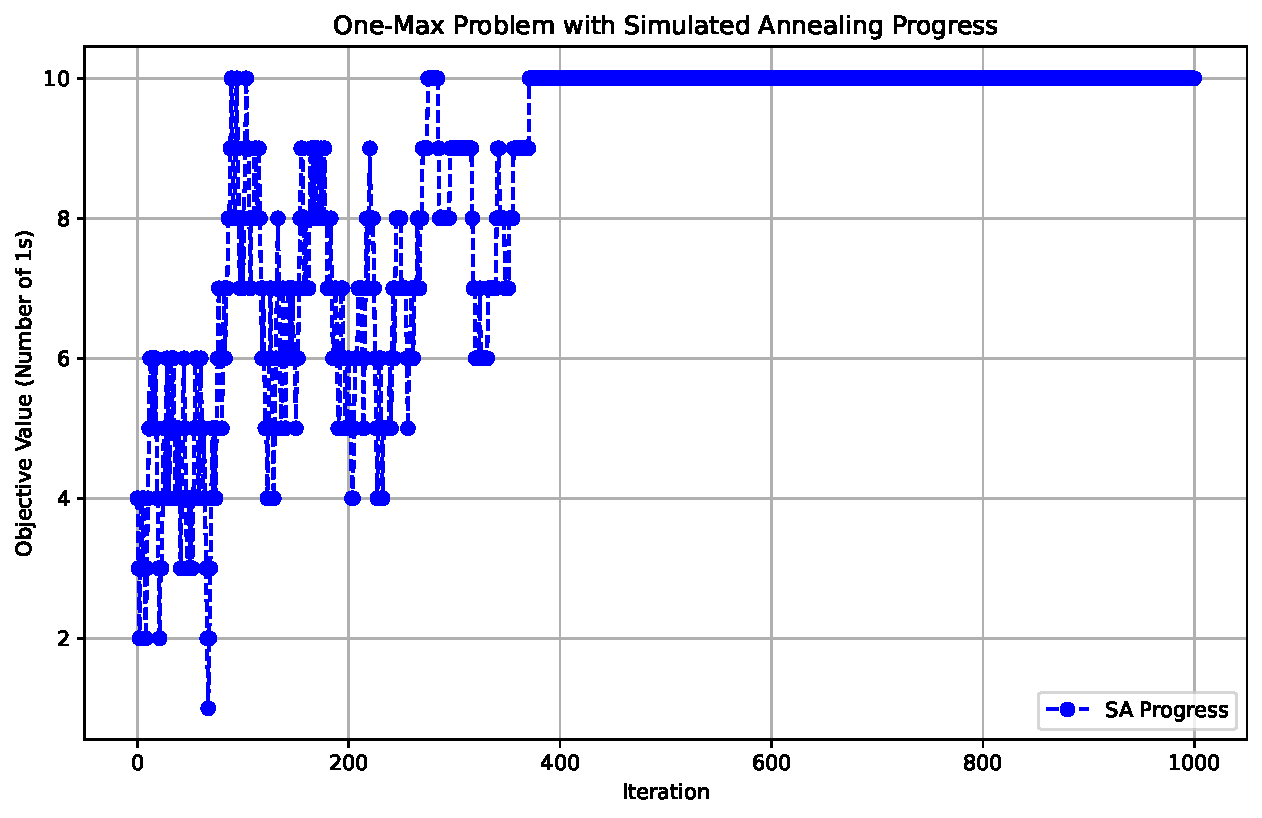
\includegraphics[keepaspectratio]{sa_files/figure-pdf/cell-9-output-2.pdf}}

\bookmarksetup{startatroot}

\chapter{SA with Ackley Function}\label{sa-with-ackley-function}

\begin{itemize}
\item
  Temperature: The algorithm starts with a high temperature, which
  decreases gradually. The algorithm starts with an initial high
  temperature (initial\_temp=10) and cools down at a rate
  (cooling\_rate=0.99) after every iteration. The temperature affects
  the likelihood of accepting worse solutions.
\item
  Acceptance of Worse Solutions: There is a probability of accepting a
  worse solution, which decreases as the temperature drops. If the new
  (neighbor) solution is worse, it is still accepted with a probability
  calculated as follows:
  \[p_a^{\text{min}} = \exp\left(\frac{\text{current\_value} - \text{neighbor\_value}}{\text{temperature}}\right)\]
\item
  This probability decreases as the temperature decreases, making it
  less likely to accept worse solutions later in the process.
\item
  Cooling Schedule: The temperature cools down over time, usually
  geometrically or exponentially. The temperature decreases by
  multiplying it by the cooling rate (0.99 in this case) at each
  iteration.
\end{itemize}

\section{Example Results}\label{example-results}

\begin{Shaded}
\begin{Highlighting}[]
\ImportTok{import}\NormalTok{ numpy }\ImportTok{as}\NormalTok{ np}
\ImportTok{import}\NormalTok{ random}
\ImportTok{import}\NormalTok{ math}
\ImportTok{import}\NormalTok{ matplotlib.pyplot }\ImportTok{as}\NormalTok{ plt}
\ImportTok{import}\NormalTok{ time}

\CommentTok{\# Define the necessary global variables}
\NormalTok{num\_evals }\OperatorTok{=} \DecValTok{1000}
\NormalTok{initial\_temp }\OperatorTok{=} \DecValTok{10}
\NormalTok{cooling\_rate }\OperatorTok{=} \FloatTok{0.99}
\NormalTok{min\_temp }\OperatorTok{=} \FloatTok{0.00001}

\CommentTok{\# Ackley function (1D)}
\KeywordTok{def}\NormalTok{ ackley(x):}
\NormalTok{    a }\OperatorTok{=} \DecValTok{20}
\NormalTok{    b }\OperatorTok{=} \FloatTok{0.2}
\NormalTok{    c }\OperatorTok{=} \DecValTok{2} \OperatorTok{*}\NormalTok{ np.pi}
\NormalTok{    term1 }\OperatorTok{=} \OperatorTok{{-}}\NormalTok{a }\OperatorTok{*}\NormalTok{ np.exp(}\OperatorTok{{-}}\NormalTok{b }\OperatorTok{*}\NormalTok{ np.sqrt(np.mean(np.square(x))))}
\NormalTok{    term2 }\OperatorTok{=} \OperatorTok{{-}}\NormalTok{np.exp(np.mean(np.cos(c }\OperatorTok{*}\NormalTok{ np.array(x))))}
    \ControlFlowTok{return}\NormalTok{ term1 }\OperatorTok{+}\NormalTok{ term2 }\OperatorTok{+}\NormalTok{ a }\OperatorTok{+}\NormalTok{ np.exp(}\DecValTok{1}\NormalTok{)}

\CommentTok{\# Initialization function (I) to set the starting point}
\KeywordTok{def}\NormalTok{ init\_sa():}
\NormalTok{    start\_x }\OperatorTok{=}\NormalTok{ random.uniform(}\OperatorTok{{-}}\DecValTok{10}\NormalTok{, }\DecValTok{10}\NormalTok{)}
    \ControlFlowTok{return}\NormalTok{ start\_x, ackley([start\_x])}

\CommentTok{\# Transition function (T)}
\KeywordTok{def}\NormalTok{ transit(current\_x):}
\NormalTok{    neighbor\_x }\OperatorTok{=}\NormalTok{ current\_x }\OperatorTok{+}\NormalTok{ random.uniform(}\OperatorTok{{-}}\DecValTok{1}\NormalTok{, }\DecValTok{1}\NormalTok{)}
    \ControlFlowTok{return}\NormalTok{ neighbor\_x}

\CommentTok{\# Determination function for SA (D)}
\KeywordTok{def}\NormalTok{ determine(neighbor\_value, current\_value, temperature):}
    \ControlFlowTok{if}\NormalTok{ neighbor\_value }\OperatorTok{\textless{}}\NormalTok{ current\_value:}
        \ControlFlowTok{return} \VariableTok{True}
    \ControlFlowTok{else}\NormalTok{:}
\NormalTok{        acceptance\_probability }\OperatorTok{=}\NormalTok{ np.exp((current\_value }\OperatorTok{{-}}\NormalTok{ neighbor\_value) }\OperatorTok{/}\NormalTok{ temperature)}
        \ControlFlowTok{return}\NormalTok{ np.random.rand() }\OperatorTok{\textless{}}\NormalTok{ acceptance\_probability}

\CommentTok{\# Simulated Annealing (SA) function}
\CommentTok{\#Evaluation Function (E)}
\KeywordTok{def}\NormalTok{ simulated\_annealing():}
\NormalTok{    current\_x, current\_value }\OperatorTok{=}\NormalTok{ init\_sa()}
\NormalTok{    best\_x, best\_value }\OperatorTok{=}\NormalTok{ current\_x, current\_value}
\NormalTok{    temperature }\OperatorTok{=}\NormalTok{ initial\_temp}
\NormalTok{    x\_history, value\_history }\OperatorTok{=}\NormalTok{ [current\_x], [current\_value]}

\NormalTok{    iterations }\OperatorTok{=} \DecValTok{0}
   
    \ControlFlowTok{while}\NormalTok{ temperature }\OperatorTok{\textgreater{}}\NormalTok{ min\_temp }\KeywordTok{and}\NormalTok{ iterations }\OperatorTok{\textless{}}\NormalTok{ num\_evals:}
\NormalTok{        neighbor\_x }\OperatorTok{=}\NormalTok{ transit(current\_x)}
\NormalTok{        neighbor\_value }\OperatorTok{=}\NormalTok{ ackley([neighbor\_x])}
        
        \ControlFlowTok{if}\NormalTok{ determine(neighbor\_value, current\_value, temperature):}
\NormalTok{            current\_x, current\_value }\OperatorTok{=}\NormalTok{ neighbor\_x, neighbor\_value}
            \ControlFlowTok{if}\NormalTok{ current\_value }\OperatorTok{\textless{}}\NormalTok{ best\_value:}
\NormalTok{                best\_x, best\_value }\OperatorTok{=}\NormalTok{ current\_x, current\_value}
        
        \CommentTok{\# Store history of x and values for plotting}
\NormalTok{        x\_history.append(current\_x)}
\NormalTok{        value\_history.append(current\_value)}

        \CommentTok{\# Cool down the temperature}
\NormalTok{        temperature }\OperatorTok{*=}\NormalTok{ cooling\_rate}
\NormalTok{        iterations }\OperatorTok{+=} \DecValTok{1}

    \ControlFlowTok{return}\NormalTok{ best\_x, best\_value, x\_history, value\_history}

\CommentTok{\# Main execution}
\NormalTok{start\_time }\OperatorTok{=}\NormalTok{ time.time()}
\NormalTok{best\_x, best\_value, x\_history, value\_history }\OperatorTok{=}\NormalTok{ simulated\_annealing()}
\NormalTok{end\_time }\OperatorTok{=}\NormalTok{ time.time()}
\NormalTok{execution\_time }\OperatorTok{=}\NormalTok{ end\_time }\OperatorTok{{-}}\NormalTok{ start\_time}

\CommentTok{\# Output (O)}
\BuiltInTok{print}\NormalTok{(}\SpecialStringTok{f"Optimal x: }\SpecialCharTok{\{}\NormalTok{best\_x}\SpecialCharTok{\}}\SpecialStringTok{"}\NormalTok{)}
\BuiltInTok{print}\NormalTok{(}\SpecialStringTok{f"Optimal value: }\SpecialCharTok{\{}\NormalTok{best\_value}\SpecialCharTok{\}}\SpecialStringTok{"}\NormalTok{)}
\BuiltInTok{print}\NormalTok{(}\SpecialStringTok{f"Execution time: }\SpecialCharTok{\{}\NormalTok{execution\_time}\SpecialCharTok{:.6f\}}\SpecialStringTok{ seconds"}\NormalTok{)}

\CommentTok{\# Plot the Ackley function and simulated annealing progress}
\NormalTok{x\_values }\OperatorTok{=}\NormalTok{ np.linspace(}\OperatorTok{{-}}\DecValTok{10}\NormalTok{, }\DecValTok{10}\NormalTok{, }\DecValTok{1000}\NormalTok{)}
\NormalTok{y\_values }\OperatorTok{=}\NormalTok{ [ackley([x]) }\ControlFlowTok{for}\NormalTok{ x }\KeywordTok{in}\NormalTok{ x\_values]}

\NormalTok{plt.figure(figsize}\OperatorTok{=}\NormalTok{(}\DecValTok{10}\NormalTok{, }\DecValTok{6}\NormalTok{))}
\NormalTok{plt.plot(x\_values, y\_values, label}\OperatorTok{=}\StringTok{"Ackley Function"}\NormalTok{, color}\OperatorTok{=}\StringTok{\textquotesingle{}b\textquotesingle{}}\NormalTok{)}
\NormalTok{plt.plot(x\_history, value\_history, marker}\OperatorTok{=}\StringTok{\textquotesingle{}o\textquotesingle{}}\NormalTok{, linestyle}\OperatorTok{=}\StringTok{\textquotesingle{}{-}{-}\textquotesingle{}}\NormalTok{, color}\OperatorTok{=}\StringTok{\textquotesingle{}red\textquotesingle{}}\NormalTok{, label}\OperatorTok{=}\StringTok{\textquotesingle{}SA Progress\textquotesingle{}}\NormalTok{)}
\NormalTok{plt.scatter(best\_x, best\_value, color}\OperatorTok{=}\StringTok{\textquotesingle{}green\textquotesingle{}}\NormalTok{, s}\OperatorTok{=}\DecValTok{100}\NormalTok{, zorder}\OperatorTok{=}\DecValTok{5}\NormalTok{, label}\OperatorTok{=}\StringTok{\textquotesingle{}Optimal Value\textquotesingle{}}\NormalTok{)}
\NormalTok{plt.title(}\StringTok{"Ackley Function in 1D with Simulated Annealing Progress"}\NormalTok{)}
\NormalTok{plt.xlabel(}\StringTok{"x"}\NormalTok{)}
\NormalTok{plt.ylabel(}\StringTok{"f(x)"}\NormalTok{)}
\NormalTok{plt.legend()}
\NormalTok{plt.grid(}\VariableTok{True}\NormalTok{)}
\NormalTok{plt.show()}
\end{Highlighting}
\end{Shaded}

\begin{verbatim}
Optimal x: 0.002038891291916256
Optimal value: 0.008376945567416971
Execution time: 0.011995 seconds
\end{verbatim}

\pandocbounded{\includegraphics[keepaspectratio]{sa_files/figure-pdf/cell-10-output-2.pdf}}

\begin{itemize}
\tightlist
\item
  Optimal x: -0.0006396808092359318

  \begin{itemize}
  \tightlist
  \item
    The value -0.00063968 represents a point very close to 0 on the
    x-axis, where the Ackley function achieves its minimum value in the
    1D case.
  \item
    The true global minimum of the Ackley function occurs at 𝑥=0, so
    this value is nearly optimal.
  \end{itemize}
\item
  Optimal value: 0.0025805153299995887

  \begin{itemize}
  \tightlist
  \item
    This is the optimal function value at the corresponding optimal x.
    It represents the Ackley function value at x=−0.00063968.
  \item
    The Ackley function's global minimum is 0, which occurs exactly at
    𝑥=0x=0. The value 0.0025805153299995887 is very close to this,
    showing that the algorithm successfully minimized the function but
    did not reach the exact minimum. This small difference can be due to
    the stochastic nature of simulated annealing and the stopping
    criteria (temperature and iterations).
  \end{itemize}
\item
  Execution time: 0.012161 seconds

  \begin{itemize}
  \tightlist
  \item
    This indicates the total time it took for the simulated annealing
    algorithm to run and find the optimal solution.
  \item
    The process completed in just 0.012 seconds, which is very fast.
    This fast execution time suggests that the algorithm quickly
    converged to a near-optimal solution, likely because the problem
    space (1D) is simple and small, and the Ackley function's shape
    guides the algorithm efficiently toward the global minimum.
  \end{itemize}
\end{itemize}

\subsection{Comparing SA to HC with Ackley
Function}\label{comparing-sa-to-hc-with-ackley-function}

\begin{itemize}
\tightlist
\item
  In an example run, I found the following results depicted in the png
  image below. The simulated annealing algorithm performed well, finding
  a solution very close to the global minimum of the Ackley function in
  a short time.
\item
  The slight deviation from the exact minimum value (0) is expected due
  to the stochastic exploration nature of simulated annealing. You can
  compare these results to the ones above under a different set seed.
\end{itemize}

\begin{figure}[H]

{\centering \pandocbounded{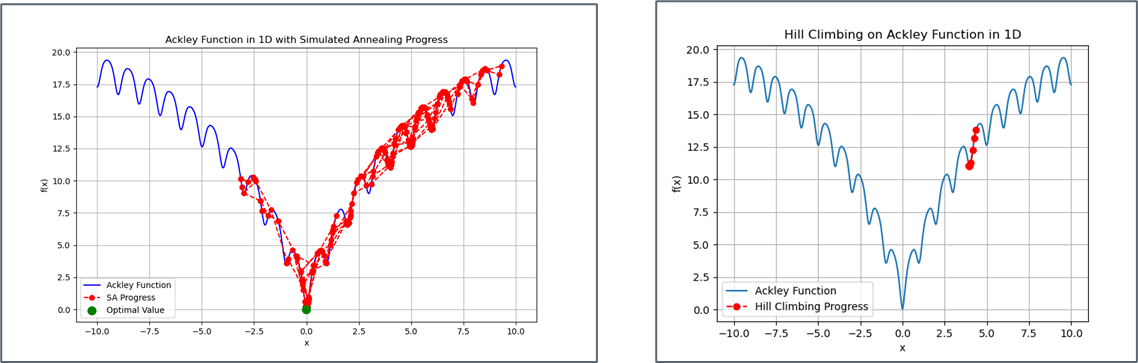
\includegraphics[keepaspectratio]{Pictures/sa4.png}}

}

\caption{Comparing HA with Ackley}

\end{figure}%

\begin{itemize}
\tightlist
\item
  Our SA model was much better than our HC model with the Ackley
  Function. Why?

  \begin{itemize}
  \tightlist
  \item
    The Ackley function is known for its multimodal landscape---it has
    many local minima and a global minimum at 𝑥=0. The landscape
    consists of a broad plateau followed by sharp drops toward the
    global minimum, making it challenging for optimization algorithms to
    find the true global minimum.
  \item
    Hill climbing can get stuck in one of the many local minima because
    it only moves to a better neighboring solution. Once it reaches a
    local minimum, it can't escape because no better solution is
    immediately available in its neighborhood.
  \item
    Simulated annealing, by contrast, has the ability to accept worse
    solutions early in the process, which allows it to escape local
    minima and continue searching for the global minimum.
  \end{itemize}
\end{itemize}

\bookmarksetup{startatroot}

\chapter{Portfolio Diversification With
SA}\label{portfolio-diversification-with-sa}

\begin{Shaded}
\begin{Highlighting}[]
\CommentTok{\#Simulated Annealing Finance Example}

\ImportTok{import}\NormalTok{ yfinance }\ImportTok{as}\NormalTok{ yf}
\ImportTok{import}\NormalTok{ numpy }\ImportTok{as}\NormalTok{ np}
\ImportTok{import}\NormalTok{ matplotlib.pyplot }\ImportTok{as}\NormalTok{ plt}
\ImportTok{import}\NormalTok{ time}

\CommentTok{\# Define the necessary global variables}
\NormalTok{max\_iterations }\OperatorTok{=} \DecValTok{1000}
\NormalTok{initial\_temp }\OperatorTok{=} \DecValTok{10}
\NormalTok{cooling\_rate }\OperatorTok{=} \FloatTok{0.995}
\NormalTok{min\_temp }\OperatorTok{=} \FloatTok{1e{-}6}

\CommentTok{\# Fetch historical stock data}
\KeywordTok{def}\NormalTok{ fetch\_data(stocks, start\_date, end\_date):}
    \ControlFlowTok{return}\NormalTok{ yf.download(stocks, start}\OperatorTok{=}\NormalTok{start\_date, end}\OperatorTok{=}\NormalTok{end\_date)[}\StringTok{\textquotesingle{}Adj Close\textquotesingle{}}\NormalTok{]}

\CommentTok{\# Evaluation Function (E): Portfolio performance calculation}
\KeywordTok{def}\NormalTok{ evaluate\_portfolio(weights, mean\_returns, cov\_matrix):}
\NormalTok{    returns }\OperatorTok{=}\NormalTok{ np.}\BuiltInTok{sum}\NormalTok{(mean\_returns }\OperatorTok{*}\NormalTok{ weights) }\OperatorTok{*} \DecValTok{252}  \CommentTok{\# Annualized returns}
\NormalTok{    risk }\OperatorTok{=}\NormalTok{ np.sqrt(np.dot(weights.T, np.dot(cov\_matrix, weights))) }\OperatorTok{*}\NormalTok{ np.sqrt(}\DecValTok{252}\NormalTok{)  }\CommentTok{\# Annualized risk}
\NormalTok{    sharpe\_ratio }\OperatorTok{=}\NormalTok{ returns }\OperatorTok{/}\NormalTok{ risk  }\CommentTok{\# Sharpe ratio}
    \ControlFlowTok{return}\NormalTok{ returns, risk, sharpe\_ratio}

\CommentTok{\# Initialization function (I)}
\KeywordTok{def}\NormalTok{ initialize\_portfolio(stocks):}
\NormalTok{    weights }\OperatorTok{=}\NormalTok{ np.random.random(}\BuiltInTok{len}\NormalTok{(stocks))}
\NormalTok{    weights }\OperatorTok{/=}\NormalTok{ np.}\BuiltInTok{sum}\NormalTok{(weights)  }\CommentTok{\# Ensure weights sum to 1}
    \ControlFlowTok{return}\NormalTok{ weights}

\CommentTok{\# Transition function (T)}
\KeywordTok{def}\NormalTok{ transition\_portfolio(weights):}
\NormalTok{    new\_weights }\OperatorTok{=}\NormalTok{ weights.copy()}
\NormalTok{    index }\OperatorTok{=}\NormalTok{ np.random.randint(}\BuiltInTok{len}\NormalTok{(weights))}
\NormalTok{    new\_weights[index] }\OperatorTok{=}\NormalTok{ np.random.uniform(}\DecValTok{0}\NormalTok{, }\DecValTok{1}\NormalTok{)}
\NormalTok{    new\_weights }\OperatorTok{/=}\NormalTok{ np.}\BuiltInTok{sum}\NormalTok{(new\_weights)  }\CommentTok{\# Ensure new weights sum to 1}
    \ControlFlowTok{return}\NormalTok{ new\_weights}

\CommentTok{\# Determination function (D)}
\KeywordTok{def}\NormalTok{ determine\_portfolio(neighbor\_sharpe, current\_sharpe, temperature):}
    \ControlFlowTok{if}\NormalTok{ neighbor\_sharpe }\OperatorTok{\textgreater{}}\NormalTok{ current\_sharpe:}
        \ControlFlowTok{return} \VariableTok{True}
    \ControlFlowTok{else}\NormalTok{:}
\NormalTok{        acceptance\_probability }\OperatorTok{=}\NormalTok{ np.exp((neighbor\_sharpe }\OperatorTok{{-}}\NormalTok{ current\_sharpe) }\OperatorTok{/}\NormalTok{ temperature)}
        \ControlFlowTok{return}\NormalTok{ np.random.rand() }\OperatorTok{\textless{}}\NormalTok{ acceptance\_probability}

\CommentTok{\# Simulated Annealing (SA) function}
\KeywordTok{def}\NormalTok{ simulated\_annealing(stocks, mean\_returns, cov\_matrix, max\_iterations, initial\_temp, cooling\_rate):}
\NormalTok{    current\_weights }\OperatorTok{=}\NormalTok{ initialize\_portfolio(stocks)}
\NormalTok{    current\_returns, current\_risk, current\_sharpe }\OperatorTok{=}\NormalTok{ evaluate\_portfolio(current\_weights, mean\_returns, cov\_matrix)}
\NormalTok{    best\_weights, best\_sharpe }\OperatorTok{=}\NormalTok{ current\_weights, current\_sharpe}
\NormalTok{    temperature }\OperatorTok{=}\NormalTok{ initial\_temp}
\NormalTok{    sharpe\_history }\OperatorTok{=}\NormalTok{ [current\_sharpe]}

\NormalTok{    iterations }\OperatorTok{=} \DecValTok{0}
    \ControlFlowTok{while}\NormalTok{ temperature }\OperatorTok{\textgreater{}}\NormalTok{ min\_temp }\KeywordTok{and}\NormalTok{ iterations }\OperatorTok{\textless{}}\NormalTok{ max\_iterations:}
\NormalTok{        neighbor\_weights }\OperatorTok{=}\NormalTok{ transition\_portfolio(current\_weights)}
\NormalTok{        neighbor\_returns, neighbor\_risk, neighbor\_sharpe }\OperatorTok{=}\NormalTok{ evaluate\_portfolio(neighbor\_weights, mean\_returns, cov\_matrix)}

        \ControlFlowTok{if}\NormalTok{ determine\_portfolio(neighbor\_sharpe, current\_sharpe, temperature):}
\NormalTok{            current\_weights, current\_sharpe }\OperatorTok{=}\NormalTok{ neighbor\_weights, neighbor\_sharpe}
            \ControlFlowTok{if}\NormalTok{ neighbor\_sharpe }\OperatorTok{\textgreater{}}\NormalTok{ best\_sharpe:}
\NormalTok{                best\_weights, best\_sharpe }\OperatorTok{=}\NormalTok{ neighbor\_weights, neighbor\_sharpe}

\NormalTok{        sharpe\_history.append(current\_sharpe)}

        \CommentTok{\# Cool down the temperature}
\NormalTok{        temperature }\OperatorTok{*=}\NormalTok{ cooling\_rate}
\NormalTok{        iterations }\OperatorTok{+=} \DecValTok{1}

    \ControlFlowTok{return}\NormalTok{ best\_weights, best\_sharpe, sharpe\_history}

\CommentTok{\# List of stocks and historical data}
\NormalTok{stocks }\OperatorTok{=}\NormalTok{ [}\StringTok{\textquotesingle{}AAPL\textquotesingle{}}\NormalTok{, }\StringTok{\textquotesingle{}GOOGL\textquotesingle{}}\NormalTok{, }\StringTok{\textquotesingle{}MSFT\textquotesingle{}}\NormalTok{, }\StringTok{\textquotesingle{}AMZN\textquotesingle{}}\NormalTok{, }\StringTok{\textquotesingle{}TSLA\textquotesingle{}}\NormalTok{, }\StringTok{\textquotesingle{}NFLX\textquotesingle{}}\NormalTok{, }\StringTok{\textquotesingle{}NVDA\textquotesingle{}}\NormalTok{, }\StringTok{\textquotesingle{}META\textquotesingle{}}\NormalTok{, }\StringTok{\textquotesingle{}DIS\textquotesingle{}}\NormalTok{, }\StringTok{\textquotesingle{}BA\textquotesingle{}}\NormalTok{]}
\NormalTok{start\_date }\OperatorTok{=} \StringTok{\textquotesingle{}2023{-}10{-}01\textquotesingle{}}
\NormalTok{end\_date }\OperatorTok{=} \StringTok{\textquotesingle{}2024{-}10{-}01\textquotesingle{}}
\NormalTok{stock\_data }\OperatorTok{=}\NormalTok{ fetch\_data(stocks, start\_date, end\_date)}
\NormalTok{returns }\OperatorTok{=}\NormalTok{ stock\_data.pct\_change().dropna()}
\NormalTok{mean\_returns }\OperatorTok{=}\NormalTok{ returns.mean()}
\NormalTok{cov\_matrix }\OperatorTok{=}\NormalTok{ returns.cov()}

\CommentTok{\# Run simulated annealing for portfolio optimization}
\NormalTok{start\_time }\OperatorTok{=}\NormalTok{ time.time()}
\NormalTok{best\_weights, best\_sharpe, sharpe\_history }\OperatorTok{=}\NormalTok{ simulated\_annealing(stocks, mean\_returns, cov\_matrix, max\_iterations, initial\_temp, cooling\_rate)}
\NormalTok{end\_time }\OperatorTok{=}\NormalTok{ time.time()}
\NormalTok{execution\_time }\OperatorTok{=}\NormalTok{ end\_time }\OperatorTok{{-}}\NormalTok{ start\_time}

\CommentTok{\# Plot the progress of the simulated annealing algorithm}
\NormalTok{plt.figure(figsize}\OperatorTok{=}\NormalTok{(}\DecValTok{10}\NormalTok{, }\DecValTok{6}\NormalTok{))}
\NormalTok{plt.plot(sharpe\_history, marker}\OperatorTok{=}\StringTok{\textquotesingle{}o\textquotesingle{}}\NormalTok{, linestyle}\OperatorTok{=}\StringTok{\textquotesingle{}{-}\textquotesingle{}}\NormalTok{, color}\OperatorTok{=}\StringTok{\textquotesingle{}b\textquotesingle{}}\NormalTok{, label}\OperatorTok{=}\StringTok{\textquotesingle{}Sharpe Ratio Progress\textquotesingle{}}\NormalTok{)}
\NormalTok{plt.title(}\StringTok{"Simulated Annealing Progress for Portfolio Optimization (Sharpe Ratio)"}\NormalTok{)}
\NormalTok{plt.xlabel(}\StringTok{"Iteration"}\NormalTok{)}
\NormalTok{plt.ylabel(}\StringTok{"Sharpe Ratio"}\NormalTok{)}
\NormalTok{plt.grid(}\VariableTok{True}\NormalTok{)}
\NormalTok{plt.legend()}
\NormalTok{plt.show()}

\CommentTok{\# Display the results}
\BuiltInTok{print}\NormalTok{(}\StringTok{"Optimized Portfolio:"}\NormalTok{)}
\ControlFlowTok{for}\NormalTok{ i, stock }\KeywordTok{in} \BuiltInTok{enumerate}\NormalTok{(stocks):}
    \BuiltInTok{print}\NormalTok{(}\SpecialStringTok{f"}\SpecialCharTok{\{}\NormalTok{stock}\SpecialCharTok{\}}\SpecialStringTok{: }\SpecialCharTok{\{}\NormalTok{best\_weights[i]}\SpecialCharTok{:.4f\}}\SpecialStringTok{"}\NormalTok{)}
\BuiltInTok{print}\NormalTok{(}\SpecialStringTok{f"Best Sharpe Ratio: }\SpecialCharTok{\{}\NormalTok{best\_sharpe}\SpecialCharTok{:.4f\}}\SpecialStringTok{"}\NormalTok{)}
\BuiltInTok{print}\NormalTok{(}\SpecialStringTok{f"Execution time: }\SpecialCharTok{\{}\NormalTok{execution\_time}\SpecialCharTok{:.6f\}}\SpecialStringTok{ seconds"}\NormalTok{)}
\end{Highlighting}
\end{Shaded}

\begin{verbatim}
[                       0%                       ][**********            20%                       ]  2 of 10 completed[**************        30%                       ]  3 of 10 completed[*******************   40%                       ]  4 of 10 completed[**********************50%                       ]  5 of 10 completed[**********************60%****                   ]  6 of 10 completed[**********************60%****                   ]  6 of 10 completed[**********************80%*************          ]  8 of 10 completed[**********************90%******************     ]  9 of 10 completed[*********************100%***********************]  10 of 10 completed
\end{verbatim}

\pandocbounded{\includegraphics[keepaspectratio]{sa_files/figure-pdf/cell-11-output-2.pdf}}

\begin{verbatim}
Optimized Portfolio:
AAPL: 0.2012
GOOGL: 0.0002
MSFT: 0.0000
AMZN: 0.0005
TSLA: 0.0000
NFLX: 0.2645
NVDA: 0.0532
META: 0.2402
DIS: 0.2365
BA: 0.0037
Best Sharpe Ratio: 2.7313
Execution time: 0.082001 seconds
\end{verbatim}

\section{Our Hill Climbing Finance Model was Better.
Why?}\label{our-hill-climbing-finance-model-was-better.-why}

\begin{itemize}
\tightlist
\item
  Hill Climbing

  \begin{itemize}
  \tightlist
  \item
    Deterministic: In each iteration, the algorithm strictly accepts a
    new portfolio only if it improves the Sharpe ratio (a measure of
    risk-adjusted returns). There's no acceptance of worse solutions.
  \item
    This results in a steady and consistent increase in the Sharpe ratio
    because the model always moves toward better solutions without
    exploring worse ones.
  \item
    Since hill climbing is greedy and deterministic, it focuses on
    continuously improving the portfolio weights in a direct manner,
    which can be more efficient for problems where the optimization
    landscape is relatively smooth or doesn't have too many local
    minima.
  \end{itemize}
\item
  Simulated Annealing:

  \begin{itemize}
  \tightlist
  \item
    Stochastic Exploration: Simulated annealing, on the other hand,
    allows for the acceptance of worse solutions, especially early in
    the process when the temperature is high. This stochastic
    exploration helps to avoid getting stuck in local minima, but it can
    sometimes lead to suboptimal moves that temporarily reduce
    performance.
  \item
    SA slowly improves the Sharpe ratio by lowering the temperature and
    becoming more selective over time. However, this can result in
    slower convergence compared to hill climbing, which directly
    improves the Sharpe ratio with each iteration.
  \item
    While simulated annealing balances exploration and exploitation, its
    performance might be slightly worse in this case because it explores
    a broader range of solutions, some of which may be worse. The
    stochastic nature may cause delays in reaching the global optimum in
    cases where the optimization problem is less prone to getting stuck
    in local minima.
  \end{itemize}
\end{itemize}

\bookmarksetup{startatroot}

\chapter{Using AI}\label{using-ai-6}

\begin{itemize}
\tightlist
\item
  Use the following prompt on a generative AI, like chatGPT, to learn
  more about the topics covered.
\item
  Metaheuristics Overview: What is a metaheuristic algorithm, and how
  does it differ from other optimization approaches like exhaustive
  search and hill climbing? Provide an example of a real-world problem
  suitable for metaheuristic algorithms.
\item
  Simulated Annealing Basics: Explain the key components of simulated
  annealing, including its transition, evaluation, and determination
  steps. Why is temperature an essential factor in the algorithm?
\item
  Exploration vs.~Exploitation: Discuss how simulated annealing balances
  exploration and exploitation during the optimization process. How does
  this compare to greedy and hill climbing algorithms?
\item
  Parameter Tuning: Why is tuning parameters like cooling schedule and
  neighborhood size crucial in simulated annealing? Suggest strategies
  for finding optimal parameter values.
\item
  Fitness Evolution: How does the cooling rate affect the trajectory of
  fitness improvement in a simulated annealing for the One-Max problem?
\item
  Solution Space Exploration: Discuss how the simulated annealing
  algorithm explores the rugged landscape of an Ackley Function and
  converges to a solution.
\item
  Industry Use Cases: Discuss real-world applications of simulated
  annealing in fields such as machine learning, logistics, and
  engineering. Why is SA particularly suited for these problems?
\item
  Challenges in SA: Reflect on the challenges of applying simulated
  annealing to real-world problems. How do computational cost and
  parameter sensitivity influence its practicality?
\item
  Algorithm Design: How does understanding the strengths and limitations
  of simulated annealing inform the design of new metaheuristic
  algorithms?
\end{itemize}

\section{Conclusions}\label{conclusions-4}

\begin{itemize}
\tightlist
\item
  Stable and Simple Search Space: In portfolio optimization, especially
  with a limited number of assets, the optimization landscape might not
  be highly rugged, making hill climbing's greedy approach more
  effective at converging quickly to a good solution.
\item
  Direct Progress: Hill climbing consistently increases the Sharpe ratio
  by only accepting better solutions, leading to slightly higher
  risk-adjusted returns over the SA model, which accepts suboptimal
  solutions early on.
\end{itemize}

\bookmarksetup{startatroot}

\chapter{Genetic Algorithms}\label{genetic-algorithms}

\bookmarksetup{startatroot}

\chapter{Genetic Algorithms}\label{genetic-algorithms-1}

\begin{itemize}
\item
  If you could `mutate' one skill you have to be even better, which one
  would it be? And if you could `crossover' with someone else's skill,
  what would you pick?
\item
  Genetic Algorithms (GAs) are optimization techniques inspired by the
  process of natural selection and evolution.
\item
  Population: A set of potential solutions (individuals) to the problem.
  Genes/Chromosomes: Each individual is represented by a chromosome (a
  string of genes), typically encoded as a binary, real-number, or
  symbolic representation.
\item
  Objective: To evolve the population toward better solutions by
  mimicking evolutionary processes such as selection, crossover, and
  mutation.
\item
  Diagram illustrating the flow of a genetic algorithm: initial
  population → selection → crossover → mutation → new population.
\end{itemize}

\section{Key Steps}\label{key-steps}

\begin{itemize}
\tightlist
\item
  Initialization: Randomly generate an initial population of individuals
  (solutions).
\item
  Selection: Choose the fittest individuals based on a fitness function
  that measures solution quality.
\item
  Crossover (Recombination): Combine parts of two parent solutions to
  create offspring (new solutions).
\item
  Mutation: Introduce random changes to an individual to maintain
  diversity and explore new parts of the solution space.
\item
  Replacement: Replace the old population with the new one, ensuring
  improvement over generations.
\item
  Termination: Continue until a stopping condition (e.g., number of
  generations or convergence) is met.
\end{itemize}

\section{Advantages}\label{advantages-1}

\begin{itemize}
\tightlist
\item
  Global Search: Capable of exploring large solution spaces and avoiding
  local optima.
\item
  Flexibility: Can be applied to many types of optimization problems,
  including those with non-linear or non-differentiable objectives.
\item
  Heuristic Nature: Useful when problem-solving methods like
  calculus-based optimization are not feasible.
\end{itemize}

\section{Genetic Algorithms Defined}\label{genetic-algorithms-defined}

\begin{itemize}
\item
  Each iteration during the convergence process is called a generation.
  GA will search more than one candidate solution per generation.
\item
  All the solutions of each generation are called a population
  indicating that there are many candidate solutions.
\item
  Each solution is called a chromosome or an individual.
\item
  Each subsolution of a solution is called a gene.
\item
  Fitness is the objective function value.
\item
  Selection is the selection based on the objective function value.
\item
  Optimization patterned on evolution

  \begin{itemize}
  \tightlist
  \item
    Maintain a population of solutions.
  \item
    ``Survival of the fittest''.
  \end{itemize}
\item
  Evolution of an improving solution

  \begin{itemize}
  \tightlist
  \item
    The population evolves over many generations.
  \item
    The fittest population members are more likely to reproduce and
    create offspring with their genetic material.
  \item
    Population fitness improves through the generations.
  \end{itemize}
\end{itemize}

\section{\texorpdfstring{The relationship between population \(s\),
chromosome \(si\), and gene
\(si,j\)}{The relationship between population s, chromosome si, and gene si,j}}\label{the-relationship-between-population-s-chromosome-si-and-gene-sij}

\begin{itemize}
\tightlist
\item
  \(s\) represents the population (a set of solutions),
\item
  \(s_i\) represents a chromosome (a solution),
\item
  \(s_{ij}\) represents a gene (a subsolution),
\item
  \(m\) represents the number of chromosomes in the population (also
  called population size, and
\item
  \(n\) represents the number of subsolutions in a chromosome.
\item
  The objective value of each chromosome will also be transformed to a
  value called the \emph{fitnes value} by a so-called fitness function.
\end{itemize}

\begin{figure}[H]

{\centering \pandocbounded{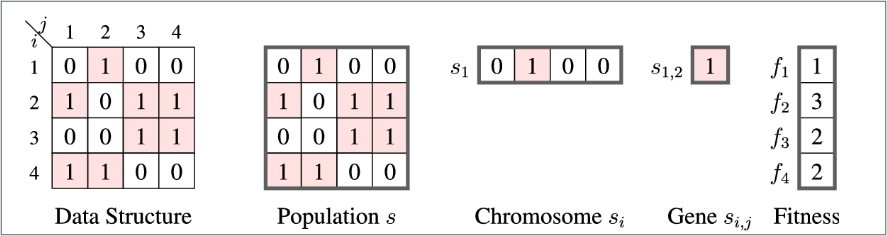
\includegraphics[keepaspectratio]{Pictures/ga1.png}}

}

\caption{Genetic Algorithm}

\end{figure}%

\subsection{The Relationships between Parents and
Children}\label{the-relationships-between-parents-and-children}

\begin{itemize}
\tightlist
\item
  Each current solution selected by the selection operator is called a
  parent, while each new candidate solution is called an offspring
  during the convergence process.
\item
  The parents s' will be selected by the selection operator from the
  current population s at iteration t. The fitness values of all the
  chromosomes will also be calculated by the selection operator.
\item
  Once the parents are selected by the selection operator, the crossover
  and mutation operators are used to generate a new population \(v\),
  which is called the offspring of the parents \(s’\).
\item
  The offspring at iteration \(t\) will become the current population s
  of iteration \(t+1\). This is referred to as the reproduction process.
\end{itemize}

\begin{figure}[H]

{\centering \pandocbounded{\includegraphics[keepaspectratio]{Pictures/ga2.png}}

}

\caption{Genetic Algorithm}

\end{figure}%

\begin{itemize}
\item
  The strategies of the selection, crossover, and mutation operators of
  GA: (a) using only the selection operator and (b) using all the three
  operators.
\item
  GA will first randomly select some of the chromosomes based on the
  fitness value of each chromosome.
\item
  Shows the situation in which only the selection operator is used,
  i.e., no other transition operators are used. In this case, the
  distribution of all the chromosomes will be shifted and changed from
  left to right on the x-axis from generation t=1 to generation t=3.
\item
  This means that the average objective value of the population will be
  increased while the variance is decreased. If GA uses only the
  selection operator but none of the transition operators (e.g.,
  crossover or mutation), it will not generate any new candidate
  solutions even though the average objective value of all the
  chromosomes is raised from 1.5 to 2.5.
\item
  Shows that if GA uses not only the selection operator to select better
  chromosomes for the next generation but also the crossover and
  mutation operators as the transition operators to generate new
  chromosomes for the population, this makes it possible for GA to find
  better candidate solutions. In this example, the average objective
  value of all the chromosomes will be increased from 1.5 to 3, while
  the best objective value will exceed 3.
\end{itemize}

\begin{figure}[H]

{\centering \pandocbounded{\includegraphics[keepaspectratio]{Pictures/ga3.png}}

}

\caption{Genetic Algorithm}

\end{figure}%

\begin{itemize}
\item
  The strategy of the transition operator of GA. (a) How the crossover
  operator works. (b) How the mutation operator works.
\item
  GA will typically apply the crossover and mutation operators to the
  chromosomes selected by the selection operator.
\item
  Two-dimensional landscape will be used as compared to one dimensional
  used in traditional methods, simulated annealing or tabu search.
\end{itemize}

\begin{figure}[H]

{\centering \pandocbounded{\includegraphics[keepaspectratio]{Pictures/ga4.png}}

}

\caption{Genetic Algorithm}

\end{figure}%

\bookmarksetup{startatroot}

\chapter{GA Algorithm}\label{ga-algorithm}

\begin{itemize}
\tightlist
\item
  Initialization: Each chromosome represents a potential solution. In
  our case, it's a binary vector indicating whether a DC is selected or
  not.
\item
  Fitness Function: The fitness of a solution is calculated based on how
  many plants can be served by the selected DCs and whether the total
  investment remains within the budget.
\item
  Selection: Select a set of solutions based on their fitness to proceed
  to the next generation.
\item
  Crossover: Perform crossover between pairs of selected solutions to
  create new offspring solutions.
\item
  Mutation: Randomly mutate some solutions to introduce diversity.
\item
  Termination: Stop when a satisfactory solution is found or after a
  fixed number of generations.
\end{itemize}

\begin{figure}[H]

{\centering \pandocbounded{\includegraphics[keepaspectratio]{Pictures/ga5.png}}

}

\caption{Genetic Algorithm}

\end{figure}%

\bookmarksetup{startatroot}

\chapter{The Probability Calculation}\label{the-probability-calculation}

\begin{itemize}
\tightlist
\item
  The probability of each chromosome being elected as a parent can be
  computed as follows: \[p_i = \frac{f_i}{\sum_{j=1}^{m} f_j}\]
\item
  Fitness \(f_i\) of member i as a proportion of sum of fitness of all
  population members, suggesting that
  \(p_i = \frac{\text{fit}}{\sum \text{fit}}\)
\end{itemize}

\section{Refining Genetic Algorithms}\label{refining-genetic-algorithms}

\begin{itemize}
\tightlist
\item
  There's no perfect setup for GA parameters. Experiment with
  combinations and monitor performance to find the best results for your
  specific problem.
\item
  GA Parameters Are Crucial: The effectiveness of GA depends heavily on
  carefully tuning parameters like population size, mutation rate, and
  the number of generations.
\item
  Population Size: For more complex problems, use larger populations
  (e.g., 1000--2000 individuals)
\item
  Mutation Rate: A low probability, typically 0.001 to 0.002 per gene.
\item
  Number of Generations: For more generations (e.g., 1000--2000
  generations).
\item
  Fitness Function: Carefully tailored to the specific problem being
  solved, as it guides the selection process.
\item
  Selection Method: rank-based linear selection or proportional
  selection can be used.
\item
  Crossover Mechanism: Single-point crossover chosen at a random
  location
\end{itemize}

\section{Fitness Function Alternatives in Heuristic
Models}\label{fitness-function-alternatives-in-heuristic-models}

\begin{itemize}
\item
  Fitness measures and selection mechanisms together determine the
  quality of offspring (solutions) in evolutionary or heuristic
  algorithms.

  \begin{itemize}
  \tightlist
  \item
    While fitness measures are problem-specific, several reasonable
    alternatives often exist.
  \item
    It's essential to tailor the fitness function to the specific goals
    of the problem (e.g., precision, speed, or robustness).
  \end{itemize}
\item
  Selection strategies (e.g., roulette wheel, tournament selection)
  could also have significant impacts on solution quality, and finding
  the right balance often requires experimentation.
\item
  Selecting the Right Fitness Function: Some fitness measures work
  significantly better than others depending on the problem.
\item
  Leverage prior knowledge or insights from similar problems to guide
  fitness function selection.
\item
  Trial and Error: Expect to experiment with different fitness measures
  to find the one that best suits your specific problem.
\item
  Common Distance Measures for Comparing Solutions to a Target:

  \begin{itemize}
  \tightlist
  \item
    Sum of Squared Differences: A measure of the total squared deviation
    of each pixel from the target, commonly used when larger errors
    should be penalized more.
  \item
    Euclidean Distance: The square root of the sum of squared
    differences, providing a more intuitive ``distance'' measure in the
    image space.
  \item
    Sum of Absolute Pixel Differences: A simpler alternative that sums
    the absolute differences for each pixel, often less sensitive to
    outliers.
  \item
    Maximum Absolute Pixel Difference: Focuses on the largest deviation,
    highlighting the worst pixel match.
  \end{itemize}
\end{itemize}

\section{Approaches to Optimize the Mutation
Rate}\label{approaches-to-optimize-the-mutation-rate}

\begin{itemize}
\tightlist
\item
  Hyperparameter Tuning: Use various fixed mutation rates and evaluate
  the performance of the GA over multiple runs to identify the best one.
  This is the simplest method but can be time-consuming as it involves
  manual experimentation.
\item
  Dynamic Mutation Rate: Adjust the mutation rate dynamically during the
  evolution process. For example, you can start with a high mutation
  rate to encourage exploration and gradually reduce it as the algorithm
  converges.
\item
  Self-Adaptive Mutation Rate: Introduce a mechanism in the GA where
  each individual in the population has its own mutation rate, which
  evolves over time. The mutation rate itself becomes part of the
  genetic material.
\item
  Cross-Validation: Use techniques like k-fold cross-validation to
  evaluate the impact of different mutation rates and find the one that
  generalizes the best.
\end{itemize}

\section{Comparing GA to SA}\label{comparing-ga-to-sa}

\begin{itemize}
\tightlist
\item
  Multiple search directions: Compared to the single-solution-based
  metaheuristic algorithms (e.g., SA) that search only one solution at a
  time, GA searches for more than one solution at a time during the
  convergence process. Since GA will search for multiple directions or
  regions at a time, its search diversity will normally be much higher
  than single-solution-based metaheuristics that search for only one
  direction or region at a time during the convergence process.
  Selection operator: Another characteristic of GA is that it uses the
  selection and fitness function operators to determine solutions to be
  searched, not just based on the objective value of each solution. This
  kind of mechanism keeps the search process of GA from looking for the
  best solution in the population all the time so that it will not
  always choose the solution with the best objective or fitness value to
  search its neighbors again and again. Consequently, GA will not easily
  get stuck in local optima at early iterations.
\item
  Crossover operator: This operator is one of the transition operators
  of GA, which plays the role of exchanging information between parent
  chromosomes, such as moving portions of the genes of a chromosome to
  another. This kind of mechanism allows GA to restructure its solutions
  to form new solutions in such a way that the structure of the new
  solutions is not confined to the structure of the initial solutions
  and may even inherit partial structures from their parents; as a
  consequence, the search process of GA will quickly jump from one
  region to another in the solution space during the convergence
  process.
\item
  Mutation operator: This operator is another transition operator of GA,
  which ensures that the search process of GA is capable of escaping
  from a local optimum by changing the value of some genes randomly. Of
  course, this kind of mechanism will also play the role of fine-tuning
  the chromosomes of GA because only a few genes will be changed at a
  time.
\end{itemize}

\bookmarksetup{startatroot}

\chapter{Genetic Algorithms}\label{genetic-algorithms-2}

\begin{itemize}
\tightlist
\item
  To compare Simulated Annealing (SA) with Genetic Algorithms (GA), we
  can implement a Genetic Algorithm for the same optimization problem
  (Ackley function) and then compare the two approaches based on:

  \begin{itemize}
  \tightlist
  \item
    Performance: Compare the final optimized values.
  \item
    Convergence Speed: How fast each algorithm converges to a solution.
  \item
    Exploration vs.~Exploitation: How each method balances searching new
    areas (exploration) versus refining the current solution
    (exploitation).
  \end{itemize}
\end{itemize}

\subsection{Genetic Algorithm for Ackley
Function}\label{genetic-algorithm-for-ackley-function}

\begin{itemize}
\tightlist
\item
  The key components of a genetic algorithm include:

  \begin{itemize}
  \tightlist
  \item
    Population: A set of candidate solutions.
  \item
    Selection: Selecting parents based on their fitness (Ackley function
    value).
  \item
    Crossover: Combining parents to produce offspring.
  \item
    Mutation: Introducing random changes to maintain diversity.
  \item
    Fitness Function: The objective function we are minimizing, which is
    the Ackley function in this case.
  \end{itemize}
\end{itemize}

\subsection{Comparison with Simulated Annealing
(SA)}\label{comparison-with-simulated-annealing-sa}

\begin{itemize}
\tightlist
\item
  Population-based vs.~Single Solution:

  \begin{itemize}
  \tightlist
  \item
    GA maintains and evolves a population of solutions.
  \item
    SA operates on a single solution and modifies it over time.
  \end{itemize}
\item
  Exploration Strategy:

  \begin{itemize}
  \tightlist
  \item
    GA uses crossover and mutation to explore the solution space,
    encouraging diversity.
  \item
    SA explores the space by making probabilistic changes to a single
    solution, allowing uphill moves early on (controlled by the
    temperature).
  \end{itemize}
\item
  Deterministic vs.~Probabilistic:

  \begin{itemize}
  \tightlist
  \item
    GA uses deterministic selection mechanisms, such as tournament
    selection, and a fixed mutation rate.
  \item
    SA uses a temperature mechanism to probabilistically accept worse
    solutions early in the search.
  \end{itemize}
\item
  Convergence:

  \begin{itemize}
  \tightlist
  \item
    GA uses generations and selection pressure to converge on the best
    solution over time.
  \item
    SA cools down gradually, converging based on the temperature
    schedule.
  \end{itemize}
\end{itemize}

\bookmarksetup{startatroot}

\chapter{GA Example Ackley}\label{ga-example-ackley}

\section{Startup Commands}\label{startup-commands}

\begin{Shaded}
\begin{Highlighting}[]
\CommentTok{\# Genetic Algorithm Ackley Example (1D)}

\ImportTok{import}\NormalTok{ numpy }\ImportTok{as}\NormalTok{ np}
\ImportTok{import}\NormalTok{ random}
\ImportTok{import}\NormalTok{ time}
\ImportTok{import}\NormalTok{ matplotlib.pyplot }\ImportTok{as}\NormalTok{ plt}

\CommentTok{\# Define the necessary global variables}
\NormalTok{pop\_size }\OperatorTok{=} \DecValTok{50}
\NormalTok{num\_generations }\OperatorTok{=} \DecValTok{100}
\NormalTok{crossover\_rate }\OperatorTok{=} \FloatTok{0.7}
\NormalTok{mutation\_rate }\OperatorTok{=} \FloatTok{0.02}
\NormalTok{num\_parents\_mating }\OperatorTok{=} \DecValTok{10}
\NormalTok{num\_players }\OperatorTok{=} \DecValTok{3}
\NormalTok{best\_obj\_val }\OperatorTok{=} \BuiltInTok{float}\NormalTok{(}\StringTok{\textquotesingle{}inf\textquotesingle{}}\NormalTok{)}
\NormalTok{best\_sol }\OperatorTok{=} \VariableTok{None}

\CommentTok{\# Ackley function (1D)}
\KeywordTok{def}\NormalTok{ ackley(x):}
\NormalTok{    a }\OperatorTok{=} \DecValTok{20}
\NormalTok{    b }\OperatorTok{=} \FloatTok{0.2}
\NormalTok{    c }\OperatorTok{=} \DecValTok{2} \OperatorTok{*}\NormalTok{ np.pi}
\NormalTok{    term1 }\OperatorTok{=} \OperatorTok{{-}}\NormalTok{a }\OperatorTok{*}\NormalTok{ np.exp(}\OperatorTok{{-}}\NormalTok{b }\OperatorTok{*}\NormalTok{ np.sqrt(np.mean(np.square(x))))}
\NormalTok{    term2 }\OperatorTok{=} \OperatorTok{{-}}\NormalTok{np.exp(np.mean(np.cos(c }\OperatorTok{*}\NormalTok{ np.array(x))))}
    \ControlFlowTok{return}\NormalTok{ term1 }\OperatorTok{+}\NormalTok{ term2 }\OperatorTok{+}\NormalTok{ a }\OperatorTok{+}\NormalTok{ np.exp(}\DecValTok{1}\NormalTok{)}
\end{Highlighting}
\end{Shaded}

\section{Initiation Function (I)}\label{initiation-function-i}

\begin{itemize}
\tightlist
\item
  A population of solutions is initialized using the init\_ga function,
  where each solution is a random number between -10 and 10, as per the
  problem domain.
\end{itemize}

\begin{Shaded}
\begin{Highlighting}[]
\CommentTok{\# Initialization function (I) to set the starting point}
\KeywordTok{def}\NormalTok{ init\_ga(pop\_size):}
    \ControlFlowTok{return}\NormalTok{ np.random.uniform(}\OperatorTok{{-}}\DecValTok{10}\NormalTok{, }\DecValTok{10}\NormalTok{, (pop\_size, }\DecValTok{1}\NormalTok{))}
\end{Highlighting}
\end{Shaded}

\section{Evaluation Function (E)}\label{evaluation-function-e}

\begin{itemize}
\tightlist
\item
  The fitness of each solution in the population is evaluated using the
  Ackley function.The best solution found so far is updated by comparing
  the current population's fitness values.
\end{itemize}

\begin{Shaded}
\begin{Highlighting}[]
\CommentTok{\# Evaluation function (E)}
\KeywordTok{def}\NormalTok{ evaluate(pop):}
    \ControlFlowTok{return}\NormalTok{ np.array([ackley(ind) }\ControlFlowTok{for}\NormalTok{ ind }\KeywordTok{in}\NormalTok{ pop])}
\end{Highlighting}
\end{Shaded}

\section{Determination (D): Update
Function}\label{determination-d-update-function}

\begin{itemize}
\tightlist
\item
  This function, update\_best\_sol, is responsible for keeping track of
  the best solution found so far in a genetic algorithm. It compares the
  fitness values of the current population (curr\_obj\_vals) to the
  global best objective value (best\_obj\_val).

  \begin{itemize}
  \tightlist
  \item
    It identifies the index (best\_idx) of the individual in the current
    population with the lowest objective value (best fitness) using
    np.argmin.
  \item
    If this individual's objective value is better (lower) than the
    current global best (best\_obj\_val), it updates best\_obj\_val to
    this new lower value and updates best\_sol to the corresponding
    individual from the current population.
  \end{itemize}
\item
  This ensures that best\_sol and best\_obj\_val always store the best
  solution and its fitness value found across all generations during the
  algorithm's execution. The use of global allows the function to modify
  these variables outside its local scope.
\end{itemize}

\begin{Shaded}
\begin{Highlighting}[]
\CommentTok{\# Update best solution function}
\KeywordTok{def}\NormalTok{ update\_best\_sol(curr\_pop, curr\_obj\_vals):}
    \KeywordTok{global}\NormalTok{ best\_sol, best\_obj\_val}
\NormalTok{    best\_idx }\OperatorTok{=}\NormalTok{ np.argmin(curr\_obj\_vals)}
    \ControlFlowTok{if}\NormalTok{ curr\_obj\_vals[best\_idx] }\OperatorTok{\textless{}}\NormalTok{ best\_obj\_val:}
\NormalTok{        best\_obj\_val }\OperatorTok{=}\NormalTok{ curr\_obj\_vals[best\_idx]}
\NormalTok{        best\_sol }\OperatorTok{=}\NormalTok{ curr\_pop[best\_idx]}
\end{Highlighting}
\end{Shaded}

\section{Determination (D): Selection
Function}\label{determination-d-selection-function}

\begin{itemize}
\tightlist
\item
  Selection: A subset of the population is selected for reproduction
  using a tournament selection process. This selection favors
  individuals with better fitness, helping to propagate good solutions.

  \begin{itemize}
  \tightlist
  \item
    This code implements a tournament selection mechanism in a genetic
    algorithm to select individuals for reproduction based on their
    fitness values.
  \item
    For each individual in the current population (curr\_pop), a
    tournament is conducted by randomly selecting a subset of
    individuals (of size num\_players) without replacement.
  \item
    Within this subset, the individual with the best fitness value
    (lowest objective value in curr\_obj\_vals) is identified using
    np.argmin and added to the selected population (selected\_pop). This
    process ensures that fitter individuals have a higher chance of
    being chosen, promoting the propagation of good solutions while
    maintaining diversity through randomness.
  \item
    The function returns the newly selected population as a NumPy array.
  \end{itemize}
\end{itemize}

\begin{Shaded}
\begin{Highlighting}[]
\CommentTok{\# Determination (D)}
\CommentTok{\# Selection function using tournament selection}
\KeywordTok{def}\NormalTok{ select(curr\_pop, curr\_obj\_vals, num\_players):}
\NormalTok{    selected\_pop }\OperatorTok{=}\NormalTok{ []}
    \ControlFlowTok{for}\NormalTok{ \_ }\KeywordTok{in} \BuiltInTok{range}\NormalTok{(}\BuiltInTok{len}\NormalTok{(curr\_pop)):}
\NormalTok{        tournament }\OperatorTok{=}\NormalTok{ np.random.choice(}\BuiltInTok{len}\NormalTok{(curr\_pop), num\_players, replace}\OperatorTok{=}\VariableTok{False}\NormalTok{)}
\NormalTok{        best\_idx }\OperatorTok{=}\NormalTok{ tournament[np.argmin(curr\_obj\_vals[tournament])]}
\NormalTok{        selected\_pop.append(curr\_pop[best\_idx])}
    \ControlFlowTok{return}\NormalTok{ np.array(selected\_pop)}
\end{Highlighting}
\end{Shaded}

\section{Transition (T): Crossover
Function}\label{transition-t-crossover-function}

\begin{itemize}
\item
  In genetic algorithms, the transition function refers to the combined
  operations of crossover and mutation that generate a new population
  (offspring) from the current population. The transition function first
  applies crossover to exchange genetic material between selected parent
  solutions, creating new offspring, and then applies mutation to
  introduce small random changes in the offspring, maintaining diversity
  and enabling exploration of the solution space. This ensures a balance
  between exploitation of good solutions (via crossover) and exploration
  of new solutions (via mutation).
\item
  Crossover: Pairs of solutions from the selected population are
  combined to create new offspring by mixing parts of the parent
  solutions.
\item
  A new population (new\_pop) is initialized as a copy of the current
  population (pop). The loop iterates over the population in pairs. For
  each pair, a random number is generated using np.random.rand(). If
  this number is less than the crossover\_rate, crossover occurs:

  \begin{itemize}
  \tightlist
  \item
    A crossover point is chosen randomly (here, using
    np.random.randint(1)), which specifies where the two parent
    solutions will exchange segments. The segments of the two parent
    solutions from the crossover point onward are swapped, creating two
    new offspring solutions.
  \item
    If the random number is greater than the crossover\_rate, no
    crossover occurs, and the parent solutions remain unchanged. The
    function returns the new\_pop containing the modified population
    after applying the crossover operation.
  \end{itemize}
\end{itemize}

\begin{Shaded}
\begin{Highlighting}[]
\CommentTok{\# Transition function (T): Crossover and Mutation}
\CommentTok{\# Crossover function (T)}
\KeywordTok{def}\NormalTok{ crossover(pop, crossover\_rate):}
\NormalTok{    new\_pop }\OperatorTok{=}\NormalTok{ pop.copy()}
    \ControlFlowTok{for}\NormalTok{ i }\KeywordTok{in} \BuiltInTok{range}\NormalTok{(}\DecValTok{0}\NormalTok{, }\BuiltInTok{len}\NormalTok{(pop) }\OperatorTok{{-}} \DecValTok{1}\NormalTok{, }\DecValTok{2}\NormalTok{):}
        \ControlFlowTok{if}\NormalTok{ np.random.rand() }\OperatorTok{\textless{}}\NormalTok{ crossover\_rate:}
\NormalTok{            crossover\_point }\OperatorTok{=}\NormalTok{ np.random.randint(}\DecValTok{1}\NormalTok{)}
\NormalTok{            new\_pop[i, crossover\_point:], new\_pop[i }\OperatorTok{+} \DecValTok{1}\NormalTok{, crossover\_point:] }\OperatorTok{=}\NormalTok{ (}
\NormalTok{                pop[i }\OperatorTok{+} \DecValTok{1}\NormalTok{, crossover\_point:], }
\NormalTok{                pop[i, crossover\_point:]}
\NormalTok{            )}
    \ControlFlowTok{return}\NormalTok{ new\_pop}
\end{Highlighting}
\end{Shaded}

\section{Transition (T): Mutation
Function}\label{transition-t-mutation-function}

\begin{itemize}
\tightlist
\item
  Mutation: Random mutations are introduced in the offspring solutions
  to maintain diversity and avoid premature convergence.
\item
  It introduces random changes to a population of solutions in a genetic
  algorithm. It iterates over each individual in the population (pop)
  and, with a probability specified by the mutation\_rate, replaces the
  current individual with a new value randomly drawn from a uniform
  distribution between -10 and 10. This random alteration helps maintain
  diversity in the population, enabling the genetic algorithm to explore
  new areas of the solution space and avoid premature convergence. The
  modified population is returned at the end of the function.
\end{itemize}

\begin{Shaded}
\begin{Highlighting}[]
\CommentTok{\# Mutation function (M)}
\KeywordTok{def}\NormalTok{ mutation(pop, mutation\_rate):}
    \ControlFlowTok{for}\NormalTok{ i }\KeywordTok{in} \BuiltInTok{range}\NormalTok{(}\BuiltInTok{len}\NormalTok{(pop)):}
        \ControlFlowTok{if}\NormalTok{ np.random.rand() }\OperatorTok{\textless{}}\NormalTok{ mutation\_rate:}
\NormalTok{            pop[i] }\OperatorTok{=}\NormalTok{ np.random.uniform(}\OperatorTok{{-}}\DecValTok{10}\NormalTok{, }\DecValTok{10}\NormalTok{)}
    \ControlFlowTok{return}\NormalTok{ pop}
\end{Highlighting}
\end{Shaded}

\section{Main Loop}\label{main-loop-3}

\begin{itemize}
\tightlist
\item
  The algorithm iterates through a fixed number of generations
  (iterations). Each generation represents an iteration of evolving the
  population to improve the solutions.
\item
  The new population (after crossover and mutation) replaces the old one
  for the next generation.
\end{itemize}

\begin{Shaded}
\begin{Highlighting}[]
\CommentTok{\# Genetic Algorithm function (D)}
\KeywordTok{def}\NormalTok{ genetic\_algorithm():}
    \KeywordTok{global}\NormalTok{ best\_sol, best\_obj\_val}
\NormalTok{    pop }\OperatorTok{=}\NormalTok{ init\_ga(pop\_size)}
    
    \ControlFlowTok{for}\NormalTok{ generation }\KeywordTok{in} \BuiltInTok{range}\NormalTok{(num\_generations):}
\NormalTok{        obj\_vals }\OperatorTok{=}\NormalTok{ evaluate(pop)}
\NormalTok{        update\_best\_sol(pop, obj\_vals)}
        
\NormalTok{        selected\_pop }\OperatorTok{=}\NormalTok{ select(pop, obj\_vals, num\_players)}
\NormalTok{        offspring\_pop }\OperatorTok{=}\NormalTok{ crossover(selected\_pop, crossover\_rate)}
\NormalTok{        mutated\_pop }\OperatorTok{=}\NormalTok{ mutation(offspring\_pop, mutation\_rate)}
        
\NormalTok{        pop }\OperatorTok{=}\NormalTok{ mutated\_pop  }
    \ControlFlowTok{return}\NormalTok{ best\_sol, best\_obj\_val}
\end{Highlighting}
\end{Shaded}

\section{Main Execution}\label{main-execution-4}

\begin{Shaded}
\begin{Highlighting}[]
\CommentTok{\# Main execution}
\NormalTok{start\_time }\OperatorTok{=}\NormalTok{ time.time()}
\NormalTok{best\_solution, best\_value }\OperatorTok{=}\NormalTok{ genetic\_algorithm()}
\NormalTok{end\_time }\OperatorTok{=}\NormalTok{ time.time()}
\NormalTok{execution\_time }\OperatorTok{=}\NormalTok{ end\_time }\OperatorTok{{-}}\NormalTok{ start\_time}
\end{Highlighting}
\end{Shaded}

\section{Output (O)}\label{output-o}

\begin{Shaded}
\begin{Highlighting}[]
\CommentTok{\# Output (O)}
\BuiltInTok{print}\NormalTok{(}\SpecialStringTok{f"Optimal solution: }\SpecialCharTok{\{}\NormalTok{best\_solution}\SpecialCharTok{\}}\SpecialStringTok{"}\NormalTok{)}
\BuiltInTok{print}\NormalTok{(}\SpecialStringTok{f"Optimal value: }\SpecialCharTok{\{}\NormalTok{best\_value}\SpecialCharTok{\}}\SpecialStringTok{"}\NormalTok{)}
\BuiltInTok{print}\NormalTok{(}\SpecialStringTok{f"Execution time for Genetic Algorithm: }\SpecialCharTok{\{}\NormalTok{execution\_time}\SpecialCharTok{:.6f\}}\SpecialStringTok{ seconds"}\NormalTok{)}

\CommentTok{\# Plot the Ackley function and genetic algorithm progress}
\NormalTok{x\_values }\OperatorTok{=}\NormalTok{ np.linspace(}\OperatorTok{{-}}\DecValTok{10}\NormalTok{, }\DecValTok{10}\NormalTok{, }\DecValTok{1000}\NormalTok{)}
\NormalTok{y\_values }\OperatorTok{=}\NormalTok{ [ackley([x]) }\ControlFlowTok{for}\NormalTok{ x }\KeywordTok{in}\NormalTok{ x\_values]}

\NormalTok{plt.figure(figsize}\OperatorTok{=}\NormalTok{(}\DecValTok{10}\NormalTok{, }\DecValTok{6}\NormalTok{))}
\NormalTok{plt.plot(x\_values, y\_values, label}\OperatorTok{=}\StringTok{"Ackley Function"}\NormalTok{, color}\OperatorTok{=}\StringTok{\textquotesingle{}b\textquotesingle{}}\NormalTok{)}
\NormalTok{plt.scatter(best\_solution[}\DecValTok{0}\NormalTok{], best\_value, color}\OperatorTok{=}\StringTok{\textquotesingle{}green\textquotesingle{}}\NormalTok{, label}\OperatorTok{=}\StringTok{\textquotesingle{}GA Best Solution\textquotesingle{}}\NormalTok{, s}\OperatorTok{=}\DecValTok{100}\NormalTok{)}
\NormalTok{plt.title(}\StringTok{"Ackley Function in 1D with Genetic Algorithm Best Solution"}\NormalTok{)}
\NormalTok{plt.xlabel(}\StringTok{"x"}\NormalTok{)}
\NormalTok{plt.ylabel(}\StringTok{"f(x)"}\NormalTok{)}
\NormalTok{plt.legend()}
\NormalTok{plt.grid(}\VariableTok{True}\NormalTok{)}
\NormalTok{plt.show()}
\end{Highlighting}
\end{Shaded}

\begin{verbatim}
Optimal solution: [-0.06049937]
Optimal value: 0.42781510242165455
Execution time for Genetic Algorithm: 0.109531 seconds
\end{verbatim}

\pandocbounded{\includegraphics[keepaspectratio]{ga_files/figure-pdf/cell-11-output-2.pdf}}

\bookmarksetup{startatroot}

\chapter{GA example One Max}\label{ga-example-one-max}

\begin{Shaded}
\begin{Highlighting}[]
\ImportTok{import}\NormalTok{ numpy }\ImportTok{as}\NormalTok{ np}
\ImportTok{import}\NormalTok{ random}
\ImportTok{import}\NormalTok{ matplotlib.pyplot }\ImportTok{as}\NormalTok{ plt}
\ImportTok{import}\NormalTok{ time}

\CommentTok{\# Define the necessary global variables}
\NormalTok{num\_bits }\OperatorTok{=} \DecValTok{10}
\NormalTok{pop\_size }\OperatorTok{=} \DecValTok{50}
\NormalTok{num\_generations }\OperatorTok{=} \DecValTok{100}
\NormalTok{crossover\_rate }\OperatorTok{=} \FloatTok{0.7}
\NormalTok{mutation\_rate }\OperatorTok{=} \FloatTok{0.01}
\NormalTok{num\_players }\OperatorTok{=} \DecValTok{3}  

\CommentTok{\# Evaluation Function (E)}
\KeywordTok{def}\NormalTok{ one\_max(sol):}
    \ControlFlowTok{return} \BuiltInTok{sum}\NormalTok{(sol)}

\CommentTok{\# Initialization function (I)}
\KeywordTok{def}\NormalTok{ initialize\_population(pop\_size, num\_bits):}
    \ControlFlowTok{return}\NormalTok{ np.random.randint(}\DecValTok{0}\NormalTok{, }\DecValTok{2}\NormalTok{, (pop\_size, num\_bits))}

\CommentTok{\# Selection function using tournament selection (D)}
\KeywordTok{def}\NormalTok{ select(population, fitness\_vals, num\_players):}
\NormalTok{    selected\_pop }\OperatorTok{=}\NormalTok{ []}
    \ControlFlowTok{for}\NormalTok{ \_ }\KeywordTok{in} \BuiltInTok{range}\NormalTok{(}\BuiltInTok{len}\NormalTok{(population)):}
\NormalTok{        tournament }\OperatorTok{=}\NormalTok{ np.random.choice(}\BuiltInTok{len}\NormalTok{(population), num\_players, replace}\OperatorTok{=}\VariableTok{False}\NormalTok{)}
\NormalTok{        best\_idx }\OperatorTok{=}\NormalTok{ tournament[np.argmax(fitness\_vals[tournament])]}
\NormalTok{        selected\_pop.append(population[best\_idx])}
    \ControlFlowTok{return}\NormalTok{ np.array(selected\_pop)}

\CommentTok{\# Crossover function (T)}
\KeywordTok{def}\NormalTok{ crossover(population, crossover\_rate):}
\NormalTok{    new\_population }\OperatorTok{=}\NormalTok{ population.copy()}
    \ControlFlowTok{for}\NormalTok{ i }\KeywordTok{in} \BuiltInTok{range}\NormalTok{(}\DecValTok{0}\NormalTok{, }\BuiltInTok{len}\NormalTok{(population) }\OperatorTok{{-}} \DecValTok{1}\NormalTok{, }\DecValTok{2}\NormalTok{):}
        \ControlFlowTok{if}\NormalTok{ random.random() }\OperatorTok{\textless{}}\NormalTok{ crossover\_rate:}
\NormalTok{            crossover\_point }\OperatorTok{=}\NormalTok{ np.random.randint(}\DecValTok{1}\NormalTok{, num\_bits)}
\NormalTok{            new\_population[i, crossover\_point:], new\_population[i }\OperatorTok{+} \DecValTok{1}\NormalTok{, crossover\_point:] }\OperatorTok{=}\NormalTok{ (}
\NormalTok{                population[i }\OperatorTok{+} \DecValTok{1}\NormalTok{, crossover\_point:], }
\NormalTok{                population[i, crossover\_point:]}
\NormalTok{            )}
    \ControlFlowTok{return}\NormalTok{ new\_population}

\CommentTok{\# Mutation function (T)}
\KeywordTok{def}\NormalTok{ mutate(population, mutation\_rate):}
    \ControlFlowTok{for}\NormalTok{ i }\KeywordTok{in} \BuiltInTok{range}\NormalTok{(}\BuiltInTok{len}\NormalTok{(population)):}
        \ControlFlowTok{for}\NormalTok{ j }\KeywordTok{in} \BuiltInTok{range}\NormalTok{(num\_bits):}
            \ControlFlowTok{if}\NormalTok{ random.random() }\OperatorTok{\textless{}}\NormalTok{ mutation\_rate:}
\NormalTok{                population[i, j] }\OperatorTok{=} \DecValTok{1} \OperatorTok{{-}}\NormalTok{ population[i, j]  }\CommentTok{\# Flip the bit}
    \ControlFlowTok{return}\NormalTok{ population}

\CommentTok{\# Genetic Algorithm function}
\KeywordTok{def}\NormalTok{ genetic\_algorithm(num\_bits, pop\_size, num\_generations, crossover\_rate, mutation\_rate):}
\NormalTok{    population }\OperatorTok{=}\NormalTok{ initialize\_population(pop\_size, num\_bits)}
\NormalTok{    best\_sol, best\_value }\OperatorTok{=} \VariableTok{None}\NormalTok{, }\DecValTok{0}
\NormalTok{    value\_history }\OperatorTok{=}\NormalTok{ []}

    \ControlFlowTok{for}\NormalTok{ generation }\KeywordTok{in} \BuiltInTok{range}\NormalTok{(num\_generations):}
\NormalTok{        fitness\_vals }\OperatorTok{=}\NormalTok{ np.array([one\_max(ind) }\ControlFlowTok{for}\NormalTok{ ind }\KeywordTok{in}\NormalTok{ population])}
\NormalTok{        best\_idx }\OperatorTok{=}\NormalTok{ np.argmax(fitness\_vals)}
        
        \CommentTok{\#Update solution (D)}
        \ControlFlowTok{if}\NormalTok{ fitness\_vals[best\_idx] }\OperatorTok{\textgreater{}}\NormalTok{ best\_value:}
\NormalTok{            best\_sol, best\_value }\OperatorTok{=}\NormalTok{ population[best\_idx], fitness\_vals[best\_idx]}
        
\NormalTok{        value\_history.append(best\_value)}
        
\NormalTok{        selected\_pop }\OperatorTok{=}\NormalTok{ select(population, fitness\_vals, num\_players)}
\NormalTok{        offspring\_pop }\OperatorTok{=}\NormalTok{ crossover(selected\_pop, crossover\_rate)}
\NormalTok{        population }\OperatorTok{=}\NormalTok{ mutate(offspring\_pop, mutation\_rate)}

    \ControlFlowTok{return}\NormalTok{ best\_sol, best\_value, value\_history}

\CommentTok{\# Main execution}
\NormalTok{start\_time }\OperatorTok{=}\NormalTok{ time.time()}
\NormalTok{best\_sol, best\_value, value\_history }\OperatorTok{=}\NormalTok{ genetic\_algorithm(num\_bits, pop\_size, num\_generations, crossover\_rate, mutation\_rate)}
\NormalTok{end\_time }\OperatorTok{=}\NormalTok{ time.time()}
\NormalTok{execution\_time }\OperatorTok{=}\NormalTok{ end\_time }\OperatorTok{{-}}\NormalTok{ start\_time}

\CommentTok{\# Output results (O)}
\BuiltInTok{print}\NormalTok{(}\SpecialStringTok{f"Best solution: }\SpecialCharTok{\{}\NormalTok{best\_sol}\SpecialCharTok{\}}\SpecialStringTok{"}\NormalTok{)}
\BuiltInTok{print}\NormalTok{(}\SpecialStringTok{f"Best fitness (one{-}max value): }\SpecialCharTok{\{}\NormalTok{best\_value}\SpecialCharTok{\}}\SpecialStringTok{"}\NormalTok{)}
\BuiltInTok{print}\NormalTok{(}\SpecialStringTok{f"Execution time: }\SpecialCharTok{\{}\NormalTok{execution\_time}\SpecialCharTok{:.6f\}}\SpecialStringTok{ seconds"}\NormalTok{)}

\CommentTok{\# Plot the progress of the genetic algorithm}
\NormalTok{plt.figure(figsize}\OperatorTok{=}\NormalTok{(}\DecValTok{10}\NormalTok{, }\DecValTok{6}\NormalTok{))}
\NormalTok{plt.plot(value\_history, marker}\OperatorTok{=}\StringTok{\textquotesingle{}o\textquotesingle{}}\NormalTok{, linestyle}\OperatorTok{=}\StringTok{\textquotesingle{}{-}\textquotesingle{}}\NormalTok{, color}\OperatorTok{=}\StringTok{\textquotesingle{}b\textquotesingle{}}\NormalTok{, label}\OperatorTok{=}\StringTok{\textquotesingle{}Best One{-}Max Value\textquotesingle{}}\NormalTok{)}
\NormalTok{plt.title(}\StringTok{"Genetic Algorithm Progress for One{-}Max Problem"}\NormalTok{)}
\NormalTok{plt.xlabel(}\StringTok{"Generation"}\NormalTok{)}
\NormalTok{plt.ylabel(}\StringTok{"Best Fitness"}\NormalTok{)}
\NormalTok{plt.grid(}\VariableTok{True}\NormalTok{)}
\NormalTok{plt.legend()}
\NormalTok{plt.show()}
\end{Highlighting}
\end{Shaded}

\begin{verbatim}
Best solution: [1 1 1 1 1 1 1 1 1 1]
Best fitness (one-max value): 10
Execution time: 0.057999 seconds
\end{verbatim}

\pandocbounded{\includegraphics[keepaspectratio]{ga_files/figure-pdf/cell-12-output-2.pdf}}

\bookmarksetup{startatroot}

\chapter{Using AI}\label{using-ai-7}

\begin{itemize}
\tightlist
\item
  Use the following prompt on a generative AI, like chatGPT, to learn
  more about the topics covered.
\item
  Concept of Genetic Algorithms: Explain the biological inspiration
  behind Genetic Algorithms. How do the concepts of selection,
  crossover, and mutation in GA mimic natural evolution?
\item
  Write a Python implementation of a Genetic Algorithm to minimize a
  simple quadratic function \(f(x) = x^2\) include steps for
  initialization, selection, crossover, mutation, and termination. How
  does the choice of parameters like mutation rate and population size
  affect the outcome?
\item
  Comparison with Simulated Annealing: Compare Genetic Algorithms to
  Simulated Annealing for solving the Ackley function. Discuss their
  strengths and weaknesses in terms of convergence speed, exploration,
  and exploitation.
\item
  Real-World Applications: Identify three real-world problems where
  Genetic Algorithms are commonly used (e.g., scheduling, vehicle
  routing, or portfolio optimization). Why are GAs particularly suited
  for these problems?
\item
  Parameter Tuning: Discuss how to determine the optimal mutation rate
  and crossover probability for a given problem. Explore techniques like
  self-adaptive mutation rates and their impact on performance.
\item
  How does the diversity of the population change as the genetic
  algorithm progresses over generations?
\end{itemize}

\bookmarksetup{startatroot}

\chapter{Conclusions}\label{conclusions-5}

\begin{itemize}
\tightlist
\item
  Our discussions on Genetic Algorithms (GA) provide a comprehensive
  exploration of one of the most versatile and biologically inspired
  optimization techniques. GA mimics the principles of natural selection
  and evolution, employing operators like selection, crossover, and
  mutation to iteratively refine solutions within a population. The
  method's ability to balance exploration (via genetic diversity) and
  exploitation (via selection pressure) makes it particularly effective
  for solving complex, non-linear, and multimodal optimization problems.
  Key advantages include its flexibility to adapt to a wide range of
  applications, such as scheduling, portfolio optimization, and function
  minimization, and its capacity to avoid local optima by maintaining a
  diverse population. However, success depends heavily on careful
  parameter tuning, including population size, mutation rate, and
  crossover probability. By comparing GA with other methods like
  Simulated Annealing, the slides highlight GA's strengths in global
  search and parallel exploration. Ultimately, Genetic Algorithms emerge
  as a powerful heuristic, especially when the optimization landscape
  demands both creativity and robustness in the search for solutions.
\end{itemize}

\bookmarksetup{startatroot}

\chapter{Summary}\label{summary}

\begin{itemize}
\item
  The course presents a structured approach to introducing heuristic
  algorithms and optimization techniques. Beginning with a broad
  overview, we highlight the significance of algorithms in diverse
  industries and introduce foundational heuristic methods, emphasizing
  their value for complex problem-solving where traditional approaches
  fall short due to scalability or computational limits: (1Intro),
  (2Algorithms), (3NumpyBasics).
\item
  The content progresses through various algorithm types: constructive
  methods like greedy algorithms, exhaustive search, and iterative
  improvement approaches, including hill climbing. Key concepts like
  local optima, plateaus, and ridges are explained alongside examples
  such as the Knapsack Problem and Traveling Salesman Problem, laying a
  foundation for understanding optimization challenges and strategies
  for improving solutions iteratively: (4Greedy); (6ExhaustiveSearch);
  and (7HillClimbing).
\item
  The later course material delves into advanced metaheuristic
  algorithms, specifically Simulated Annealing (SA) and Genetic
  Algorithms (GA). SA is explained with its cooling schedule and
  probabilistic acceptance of suboptimal solutions, which help avoid
  local optima. GA is described through its evolutionary
  process---selection, crossover, and mutation---illustrating how
  populations of solutions evolve toward optimality over generations.
\item
  The advantages and disadvantages of each approach are covered, along
  with the importance of tuning parameters for effective convergence.
  This framework not only familiarizes students with the mechanics of
  each method but also stresses the trade-offs involved, preparing them
  to apply these techniques to benchmark problems such as the Ackley and
  OneMax functions: (5BenchmarkProblems); (8-9SimulatedAnnealing); and
  (10-11GeneticAlgorithms)
\end{itemize}

\bookmarksetup{startatroot}

\chapter{Required Reading Materials}\label{required-reading-materials}

\begin{itemize}
\tightlist
\item
  Tsai, C.-W., \& Chiang, M.-C. (2023). \emph{Handbook of metaheuristic
  algorithms}. Academic Press. Retrieved from
  \url{https://learning.oreilly.com/library/view/handbook-of-metaheuristic/9780443191091/}
\end{itemize}

\bookmarksetup{startatroot}

\chapter{Recommended Further Reading
Materials}\label{recommended-further-reading-materials}

\begin{itemize}
\tightlist
\item
  Erwig, M. (2017). Once upon an algorithm: How stories explain
  computing. The MIT Press.
\item
  Holland, 1992 J.H. Holland, Adaptation in Natural and Artificial
  Systems. Cambridge, MA: MIT Press; 1992.
\item
  Holland, 1962 J.H. Holland, Outline for a logical theory of adaptive
  systems, Journal of the ACM 1962;9:297--314.
\item
  Holland, 1975 J.H. Holland, Adaptation in Natural and Artificial
  Systems. Ann Arbor, MI: University of Michigan Press; 1975.
\item
  Steiner, C. (2012). Automate this: How algorithms came to rule our
  world. Portfolio/Penguin.
\end{itemize}




\end{document}
